\documentclass[11pt,a4paper,oneside,openany]{book}
\usepackage[T1]{fontenc}
\usepackage[utf8]{inputenc}
\usepackage{lmodern}
\usepackage[a4paper,margin=23mm,headheight=15pt,footskip=12mm]{geometry}
\usepackage{microtype}
\usepackage{amsmath,amssymb,mathtools}
\usepackage{graphicx,xcolor}
\usepackage{booktabs,tabularx,longtable,array}
\usepackage{enumitem,needspace}
\usepackage{listings}
\usepackage{tikz,pgfplots}
\usetikzlibrary{arrows.meta,calc,angles,quotes,positioning,decorations.pathreplacing,patterns,fit,backgrounds}
\pgfplotsset{compat=1.18}
\usepackage[most]{tcolorbox}
\usepackage{fancyhdr}
\usepackage{hyperref}
\usepackage{bookmark}
\definecolor{manualink}{HTML}{173047}
\definecolor{manualblue}{HTML}{1D5B93}
\definecolor{manualteal}{HTML}{0F807D}
\definecolor{manualorange}{HTML}{C46A20}
\definecolor{manualred}{HTML}{B43A42}
\definecolor{manualmuted}{HTML}{647486}
\definecolor{manuallight}{HTML}{F2F6F9}
\hypersetup{colorlinks=true,linkcolor=manualblue,urlcolor=manualteal,
  pdftitle={nurbspath - Illustrated C++20 Reference Manual},
  pdfauthor={nurbspath contributors},pdfsubject={Entities, creation, algorithms, and examples}}
\DeclareRobustCommand{\api}[1]{\texttt{\detokenize{#1}}}
\newcommand{\figref}[1]{Figure~\ref{#1}}
\newcommand{\secref}[1]{Section~\ref{#1}}
\newcommand{\Real}{\mathbb{R}}
\newcommand{\R}{\mathbb{R}}
\newcommand{\vect}[1]{\boldsymbol{#1}}
\newcolumntype{Y}{>{\raggedright\arraybackslash}X}
\newtcolorbox{manualnote}[1][Practical note]{enhanced,breakable,
  colback=manuallight,colframe=manualteal!50,coltitle=manualink,
  colbacktitle=manualteal!8,fonttitle=\sffamily\bfseries,title={#1},
  boxrule=.5pt,arc=1.5mm,left=3mm,right=3mm,top=2mm,bottom=2mm,
  before upper={\raggedright}}
\lstdefinestyle{cpp}{language=C++,basicstyle=\ttfamily\small,
  keywordstyle=\color{manualblue}\bfseries,commentstyle=\color{manualmuted},
  stringstyle=\color{manualteal},backgroundcolor=\color{manuallight},
  frame=single,rulecolor=\color{manualblue!20},framesep=6pt,
  columns=fullflexible,keepspaces=true,showstringspaces=false,
  breaklines=true,breakatwhitespace=false,tabsize=2,
  aboveskip=9pt,belowskip=9pt}
\lstdefinestyle{apireference}{style=cpp,basicstyle=\ttfamily\footnotesize,
  frame=none,backgroundcolor=\color{manuallight},aboveskip=3pt,
  belowskip=2pt,framesep=3pt}
\lstdefinestyle{plain}{style=cpp,language={},basicstyle=\ttfamily\small}
\lstset{style=cpp}
\tikzset{axis/.style={-{Stealth[length=2mm]},draw=manualmuted,thin},
  vector/.style={-{Stealth[length=2.3mm]},draw=manualblue,very thick},
  curve/.style={draw=manualblue,very thick},
  control/.style={draw=manualmuted,dashed,thin},
  guide/.style={draw=manualmuted,densely dashed,thin},
  point/.style={circle,fill=manualink,inner sep=1.5pt},
  surface/.style={draw=manualteal,fill=manualteal!9},
  every node/.style={font=\small}}
\pgfplotsset{every axis/.append style={
  tick label style={font=\footnotesize},label style={font=\small},
  legend style={font=\footnotesize,draw=none,fill=white},
  axis line style={manualmuted},tick style={manualmuted},
  grid style={manualmuted!15},width=.88\linewidth,height=6.3cm,
  unbounded coords=jump}}
\setlist{itemsep=3pt,topsep=5pt,leftmargin=*}
\setlength{\parindent}{0pt}
\setlength{\parskip}{5pt plus 1pt}
\setlength{\emergencystretch}{2em}
\setcounter{tocdepth}{1}
\setcounter{secnumdepth}{2}
\renewcommand{\arraystretch}{1.16}
\pagestyle{fancy}
\fancyhf{}
\fancyhead[L]{\sffamily\small\color{manualmuted}nurbspath / Illustrated reference}
\fancyhead[R]{\sffamily\small\color{manualmuted}\nouppercase{\leftmark}}
\fancyfoot[L]{\sffamily\footnotesize\color{manualmuted}C++20 / library \ManualVersion}
\fancyfoot[R]{\sffamily\small\thepage}
\renewcommand{\headrulewidth}{.3pt}
\renewcommand{\chaptermark}[1]{\markboth{\thechapter\quad #1}{}}
\fancypagestyle{plain}{\fancyhf{}\fancyfoot[R]{\sffamily\small\thepage}\renewcommand{\headrulewidth}{0pt}}
\InputIfFileExists{pictures/reference_values.tex}{}{}
\providecommand{\ManualVersion}{0.4.3}
\InputIfFileExists{pictures/revision.tex}{}{}
\providecommand{\ManualRevision}{source snapshot}
\raggedbottom

\begin{document}
\hypersetup{pageanchor=false}
\begin{titlepage}
\thispagestyle{empty}
\vspace*{12mm}
{\sffamily\bfseries\color{manualteal}\large LIBRARY MANUAL / FIRST EDITION\par}
\vspace{9mm}
{\sffamily\bfseries\color{manualink}\fontsize{43}{47}\selectfont nurbspath\par}
\vspace{4mm}
{\sffamily\color{manualblue}\LARGE An illustrated C++20 reference\par}
\vspace{7mm}
{\large Entities, construction, NURBS paths,\par numerical queries, and output\par}
\vspace{12mm}
\begin{center}
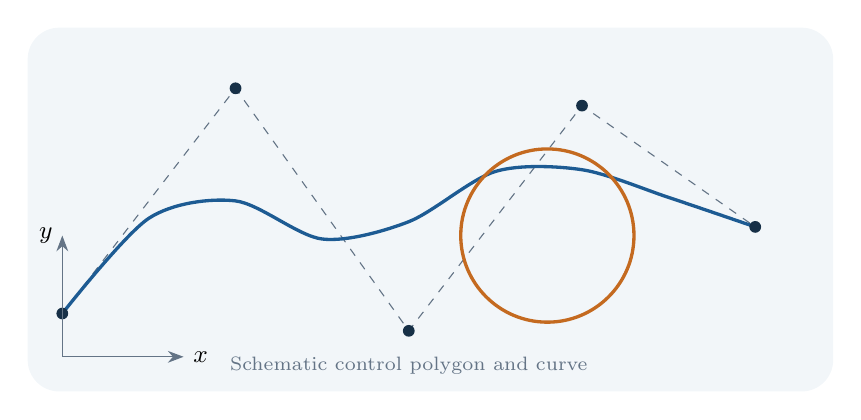
\begin{tikzpicture}[x=2.2cm,y=2.2cm]
  \fill[manuallight,rounded corners=4mm] (-.2,-.45) rectangle (4.45,1.65);
  \draw[control] (0,0)--(1,1.3)--(2,-.1)--(3,1.2)--(4,.5);
  \draw[curve] plot[smooth] coordinates {(0,0)(.5,.55)(1,.65)(1.5,.43)(2,.53)(2.5,.82)(3,.83)(3.5,.67)(4,.5)};
  \foreach \p in {(0,0),(1,1.3),(2,-.1),(3,1.2),(4,.5)} \node[point] at \p {};
  \draw[manualorange,very thick] (2.8,.45) circle (.5);
  \draw[axis] (0,-.25)--(.7,-.25) node[right] {$x$};
  \draw[axis] (0,-.25)--(0,.45) node[left] {$y$};
  \node[manualmuted,font=\scriptsize] at (2.0,-.30) {Schematic control polygon and curve};
\end{tikzpicture}
\end{center}
\vfill
{\sffamily\bfseries Library version \ManualVersion\par}
{\color{manualmuted}Source revision \texttt{\ManualRevision}\par}
{\color{manualmuted}27 October 2026\par}
\vspace{5mm}
{\small Standalone experimental manual. All figures are TikZ/PGFPlots drawings;
the sampled reference curves and query results are calculated by nurbspath.
This document is built independently of the project CMake configuration.\par}
\end{titlepage}

\hypersetup{pageanchor=true}
\frontmatter
\InputIfFileExists{intro.tex}{}{}
\tableofcontents
\listoffigures
\mainmatter
\chapter{Reading and using the library}\label{chap:foundations}
\section{Scope and a first working program}
\api{nurbspath} is a dependency-free, header-only C++20 library. Its geometry
types use a scalar template parameter constrained by \api{std::floating_point};
\api{float}, \api{double}, and \api{long double} are valid choices. Include
\api{nurbspath/nurbspath.hpp} for the complete API or a focused public header
for a smaller translation unit.

This manual describes the source snapshot printed on the title page. Chapters
\ref{chap:entities}--\ref{chap:output} explain the public operations by purpose;
Appendix~\ref{chap:reference} records individual overloads, defaults, result
types, and public data members extracted from those headers. Internal
\api{nurbspath::detail} helpers are implementation, not a public contract.

\begin{lstlisting}
#include <nurbspath/config.hpp>
#include <nurbspath/nurbspath.hpp>
#include <iomanip>
#include <iostream>

int main() {
    namespace np = nurbspath;
    using REAL = double;
    const np::circle2<REAL> circle({0.0, 0.0}, 1.0);
    const np::ray2<REAL> ray({-3.0, 0.0}, {2.0, 0.0});
    const auto result = np::intersect(ray, circle);
    std::cout << std::scientific << std::setprecision(4);
    for (const auto& hit : result.points) {
        std::cout << "s=" << hit.s << " point=" << hit.point << '\n';
    }
}
\end{lstlisting}
\begin{lstlisting}[style=plain]
s=1.0000e+00 point=-1.0000e+00 0.0000e+00
s=2.0000e+00 point=1.0000e+00 0.0000e+00
\end{lstlisting}
The ray direction has length two, so the native parameter is half the travelled
world distance. Compile this program directly with the source include directory:
\begin{lstlisting}[style=plain]
c++ -std=c++20 -I../include first_query.cpp -o first_query
\end{lstlisting}
This command is shown relative to the manual directory. The manual's own
reproducible reference programs and build instructions are in
Appendix~\ref{chap:reproduction}.

\section{Two independent Cartesian worlds}
\begin{tabularx}{\linewidth}{@{}lYY@{}}
\toprule
Concept & Independent 2D world & Shared 3D world\\
\midrule
Position & \api{point2<REAL>} & \api{point3<REAL>}\\
Offset or direction & \api{vector2<REAL>} & \api{vector3<REAL>}\\
Forward line & \api{ray2<REAL>} & \api{ray3<REAL>}\\
Round surface & \api{circle2<REAL>} & \api{sphere3<REAL>}\\
Rational path & \api{nurbs_spline2<REAL>} & \api{nurbs_spline3<REAL>}\\
Array-backed path & \api{nurbs_arr_spline2}\newline\api{<REAL>} & \api{nurbs_arr_spline3}\newline\api{<REAL>}\\
Plane & No 2D plane entity & \api{plane3<REAL>}\\
\bottomrule
\end{tabularx}

A point represents a location; a vector represents an offset or direction.
Point subtraction gives a vector, point plus vector gives a point, and vector
arithmetic remains vector arithmetic. A 2D entity does not implicitly become
a 3D entity. The explicit bridge is \api{project(plane, entity2)}, described in
Chapter~\ref{chap:entities}. Queries on 2D entities compute entirely in 2D.

\section{Units, parameters, and tolerances}
The library does not prescribe metres, millimetres, or another length unit.
Choose one consistent world unit. Angles are in radians. Display widths and
text sizes are separate consumer-selected display units.

\begin{tabularx}{\linewidth}{@{}lYY@{}}
\toprule
Entity & Parameter domain & Meaning\\
\midrule
Ray & $s\geq0$ for forward queries & $O+s\vect d$; direction is unnormalised.\\
Spline & $[t_p,t_C]$ & Active knot interval; $C$ is the number of controls.\\
Circle & $u\in[0,2\pi)$ & Counterclockwise angle from positive $x$.\\
Sphere & $u\in[0,2\pi)$, $v\in[-\pi/2,\pi/2]$ & Longitude and latitude.\\
Plane & $(u,v)\in\Real^2$ & Orthonormal local coordinates.\\
\bottomrule
\end{tabularx}

The ray's evaluation formula can be evaluated for negative $s$, but intersection
queries treat it as a forward half-line. Spline parameters remain native:
interpolation preserves the supplied stations, and plane embedding preserves
the same $s$ values. A spline parameter is not automatically a physical arc
length everywhere between interpolation stations.

\begin{manualnote}[What a tolerance controls]
Definition tolerances validate entity construction and parameter boundaries.
\api{numerical_settings<REAL>} separately controls function residuals,
parameter intervals, iteration counts, and sampling density. These quantities
have different units. Sampling-based intersections, spline distances, and arc
length estimates depend on their chosen sample counts; a finite sampling run
does not prove a continuous global result for every possible curve.
\end{manualnote}

\section{Values, shared ownership, and checked editing}
Construct entities as ordinary values for simple ownership. The
\api{make_*} functions in \api{creators.hpp} mirror geometry constructors and
return \api{std::shared_ptr} objects. They preserve constructor validation and
exceptions. They do not introduce a common geometry base class.

Ordinary spline definitions are private and use checked, atomic setters.
Failed edits leave the old definition intact. Array-backed alternatives
deliberately expose a \api{std::valarray<REAL>}; direct replacement is allowed,
so geometry operations validate the current storage and do not rely on stale
endpoint caches. References returned by getters follow their documented
invalidation rules.

\section{How the worked figures were made}
Simple vector, plane, and circle constructions are drawn directly in TikZ.
Curves, analytic derivatives, interpolation points, intersections, and closest
points use data generated by \api{pictures/generate_reference.cpp}, which
includes the library itself. The generator checks its results before writing
the coordinate files. The stored plot coordinates and displayed output use
scientific notation with at most four decimal places. The calculations are
performed in full \api{double} precision before display rounding.

The figures distinguish a mathematical curve from its drawn approximation:
PGFPlots connects library-evaluated points. Its smooth appearance is not an
extra numerical guarantee. This manual requires no image downloads, external
plotting service, shell escape, or TikZ externalisation.

\chapter{Entities and elementary geometry}
\label{chap:entities}

An entity carries both a geometric meaning and a dimension. A \api{point2}
is a position in the native 2D world; a \api{vector2} is a displacement in
that world. Their 3D counterparts have the same distinction. All geometry
templates take a floating-point scalar type, written \api{REAL}; the examples
in this chapter use \api{double}.

\begin{table}[htbp]
\centering
\caption{Entity families and their native parameters.}
\begin{tabularx}{\linewidth}{@{}lXl@{}}
\toprule
Entity & Meaning & Parameters \\
\midrule
\api{point2}, \api{point3} & Cartesian position & coordinates \\
\api{vector2}, \api{vector3} & Offset or direction & components \\
\api{ray2}, \api{ray3} & Forward half-line & $s\geq0$ \\
\api{circle2} & Circle in the native 2D world & angle $u$ \\
\api{sphere3} & Spherical surface in 3D & longitude $u$, latitude $v$ \\
\api{plane3} & Infinite oriented plane in 3D & local distances $u,v$ \\
\api{nurbs_spline2}, \api{nurbs_spline3} & Rational B-spline curve & native $s$ \\
\api{nurbs_arr_spline2}, \api{nurbs_arr_spline3} & Array-backed curve alternative & native $s$ \\
\bottomrule
\end{tabularx}
\end{table}

There is no \api{plane2}. A 2D point is not implicitly a 3D point with a
zero Z coordinate. The explicit bridge \api{project(plane, entity2)} embeds a
2D entity using a specified \api{plane3}; its geometric meaning is described
in Chapter~\ref{chap:algorithms}. Spline definitions and their analytic
derivatives are developed in Chapter~\ref{chap:splines}.

\section{Points: positions and translations}

\api{point2<REAL>} and \api{point3<REAL>} are aggregates with public,
zero-initialized coordinates \api{x}, \api{y}, and, for 3D, \api{z}.
Aggregate initialization and \api{origin()} provide their creation calls:

\begin{lstlisting}[language=C++]
using namespace nurbspath;
point2<double> a{1.0, 2.0};
point3<double> b{1.0, 2.0, 3.0};
const auto o2 = point2<double>::origin();
const auto o3 = point3<double>::origin();
\end{lstlisting}

\api{operator[]} gives mutable or constant coordinate access in X/Y/Z
order, starting at index zero; an invalid index throws
\api{std::out_of_range}. \api{operator==} compares coordinates exactly.
Use \api{approximately_equal(other, tolerance)} when a Euclidean position
tolerance is intended.

Subtracting two points gives the vector from the right operand to the left.
Adding or subtracting a vector translates a point; \api{+=} and \api{-=}
are the in-place forms. Both \api{point + vector} and
\api{vector + point} are available. Two points cannot be added, and a point
cannot be scaled as though it were a displacement.

\begin{figure}[htbp]
\centering
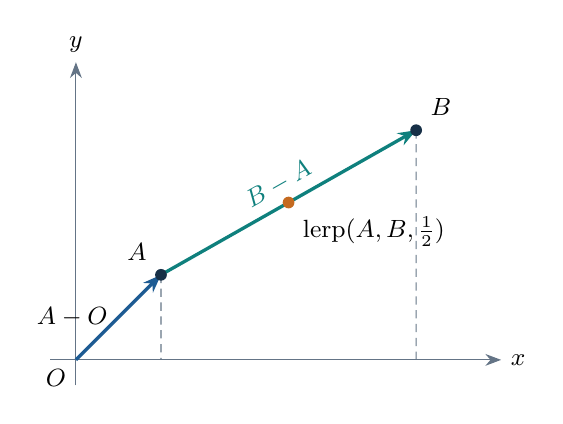
\begin{tikzpicture}[scale=1.08]
\draw[axis] (-.3,0)--(5,0) node[right]{$x$};
\draw[axis] (0,-.3)--(0,3.5) node[above]{$y$};
\coordinate (O) at (0,0); \coordinate (A) at (1,1);
\coordinate (B) at (4,2.7); \coordinate (M) at (2.5,1.85);
\draw[guide] (A)--(1,0); \draw[guide] (B)--(4,0);
\draw[vector] (O)--(A) node[midway,left]{$A-O$};
\draw[vector,manualteal] (A)--(B) node[midway,above,sloped]{$B-A$};
\node[point,label=above left:$A$] at (A) {};
\node[point,label=above right:$B$] at (B) {};
\node[point,fill=manualorange,label=below right:{$\operatorname{lerp}(A,B,\tfrac12)$}] at (M) {};
\node[below left] at (O) {$O$};
\end{tikzpicture}
\caption{Positions are anchored in a Cartesian world. The difference $B-A$
is a displacement; adding that displacement to $A$ recovers $B$.}
\label{fig:point-displacement}
\end{figure}

\begin{lstlisting}[language=C++]
const point3<double> first{1.0, 1.0, 0.0};
const point3<double> second{4.0, 3.0, 0.0};
const vector3<double> offset = second - first;
const point3<double> translated = first + offset;
const point3<double> middle = lerp(first, second, 0.5);
const double separation = distance(first, second);
\end{lstlisting}

\api{lerp(first, second, fraction)} evaluates
$P_0+t(P_1-P_0)$ in either world. It permits extrapolation: fractions below
zero or above one continue along the same line. \api{distance} returns
Euclidean distance and \api{distance_squared} returns its square without a
square root. These free functions take two points from the same world.

The point members \api{magnitude()} and \api{manhattan_distance()} measure
distance from the Cartesian origin, respectively
$\sqrt{x^2+y^2+z^2}$ and $|x|+|y|+|z|$, with the Z term omitted in 2D.
They do not measure distance from a user-selected local origin.

\begin{manualnote}[Explicit component copying]
A same-world vector may be assigned to a point. For example,
\api{b = vector3<double>{1, 2, 3}} replaces the point coordinates with those
components. This is a coordinate-copy operation, not a translation. Point
and vector types nevertheless remain distinct, and no dimension conversion
is introduced by this assignment.
\end{manualnote}

\section{Vectors: directions and their components}

Vectors have public, zero-initialized components and the same checked indexed
access and exact equality as points. Their constructors are:

\begin{minipage}{\linewidth}
\begin{lstlisting}[language=C++]
vector2<double> zero2;
vector2<double> v2{3.0, 4.0};
vector3<double> zero3;
vector3<double> v3{1.0, 2.0, 3.0};
vector3<double> from_position{point3<double>{1.0, 2.0, 3.0}};
\end{lstlisting}
\end{minipage}

The constructors from entities are explicit. A \api{vector2} constructed
from a \api{point2}, \api{circle2}, or \api{ray2} copies, respectively,
the point coordinates, circle center, or ray origin. A \api{vector3}
constructed from a \api{point3}, \api{sphere3}, \api{plane3}, or
\api{ray3} copies the point, center, plane origin, or ray origin. In
particular, constructing a vector from a ray does not extract its direction;
use \api{direction()} for that purpose.

\subsection{Algebra and length}

For both vector types, unary plus and minus, vector addition and subtraction,
scalar multiplication in either order, and scalar division are available.
Their compound forms are \api{+=}, \api{-=}, \api{*=}, and \api{/=}.
Division by an exactly zero scalar throws \api{std::domain_error}.

\begin{table}[htbp]
\centering
\caption{Vector operations common to 2D and 3D. Here $a$ and $b$ have the
same vector type and $t$ is a scalar.}
\begin{tabularx}{\linewidth}{@{}lX@{}}
\toprule
Call & Result or use \\
\midrule
\api{a.dot(b)}, \api{dot(a, b)} & Scalar inner product $a\cdot b$. \\
\api{a.cross(b)}, \api{cross(a, b)} & Signed scalar area in 2D; right-handed perpendicular vector in 3D. \\
\api{a.length_squared()} & $a\cdot a$. \\
\api{a.length()} & Euclidean length, evaluated with \api{std::hypot}. \\
\api{a.is_near_zero(tolerance)} & Whether squared length is at most the squared tolerance. \\
\api{a.normalized(tolerance)} & New unit vector; throws for a length at or below the tolerance. \\
\api{a.normalize()} & Normalize in place using the default tolerance; unchanged if it fails. \\
\api{a.component_product(b)} & Product of corresponding components. \\
\api{a.min_component()}, \api{a.max_component()} & Smallest or largest signed component. \\
\api{a.approximately_equal(b, tolerance)} & Euclidean component-space difference within tolerance. \\
\api{lerp(a, b, t)} & $(1-t)a+tb$; extrapolation is permitted. \\
\bottomrule
\end{tabularx}
\end{table}

\api{zero()}, \api{unit_x()}, and \api{unit_y()} are static vector
constructors; \api{vector3} also has \api{unit_z()}.
\api{default_tolerance()} is $64$ times the machine epsilon of
\api{REAL}. This absolute tolerance is a convenient arithmetic default;
applications should supply a meaningful length tolerance when their scale
requires it.

In 2D, $a\times b=a_xb_y-a_yb_x$ is positive when $b$ lies
counterclockwise from $a$ through an angle below $\pi$.
\api{perpendicular_left()} returns $(-a_y,a_x)$ and
\api{perpendicular_right()} returns $(a_y,-a_x)$; neither normalizes.
In 3D, the cross product follows the right-hand rule.

\begin{figure}[htbp]
\centering
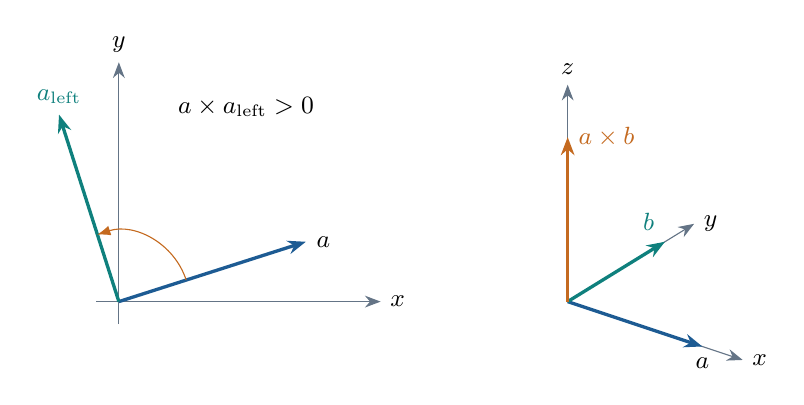
\begin{tikzpicture}[scale=.95]
\begin{scope}
\draw[axis] (-.3,0)--(3.5,0) node[right]{$x$};
\draw[axis] (0,-.3)--(0,3.2) node[above]{$y$};
\draw[vector] (0,0)--(2.5,.8) node[right]{$a$};
\draw[vector,manualteal] (0,0)--(-.8,2.5) node[above]{$a_\mathrm{left}$};
\draw[manualorange,-{Latex}] (.9,.288) arc[start angle=18,end angle=108,radius=.945];
\node at (1.7,2.6) {$a\times a_\mathrm{left}>0$};
\end{scope}
\begin{scope}[shift={(6,0)},x={(.9cm,-.3cm)},y={(.65cm,.4cm)},z={(0cm,1cm)}]
\draw[axis] (0,0,0)--(2.6,0,0) node[right]{$x$};
\draw[axis] (0,0,0)--(0,2.6,0) node[right]{$y$};
\draw[axis] (0,0,0)--(0,0,2.9) node[above]{$z$};
\draw[vector] (0,0,0)--(2,0,0) node[below]{$a$};
\draw[vector,manualteal] (0,0,0)--(0,2,0) node[above left]{$b$};
\draw[vector,manualorange] (0,0,0)--(0,0,2.2) node[right]{$a\times b$};
\end{scope}
\end{tikzpicture}
\caption{The 2D perpendicular operation and the 3D cross product have
different return types. Both retain orientation information.}
\end{figure}

\subsection{Projection, rejection, reflection, and angles}

For a nonzero axis $b$, the member \api{a.projected_onto(b, tolerance)}
computes
\[
 a_{\parallel}=\frac{a\cdot b}{b\cdot b}\,b,
 \qquad
 a_{\perp}=a-a_{\parallel}.
\]
\api{a.rejected_from(b, tolerance)} returns $a_{\perp}$.
The axis need not be normalized. Both calls reject an axis whose squared
length is at or below the squared tolerance.

\api{a.reflected(normal, tolerance)} computes
$a-2(a\cdot\widehat n)\widehat n$. Its argument is the normal to the
reflecting line in 2D or plane in 3D. Passing the direction of the reflecting
line would describe a different reflection. A near-zero normal throws
\api{std::domain_error}.

\begin{figure}[htbp]
\centering
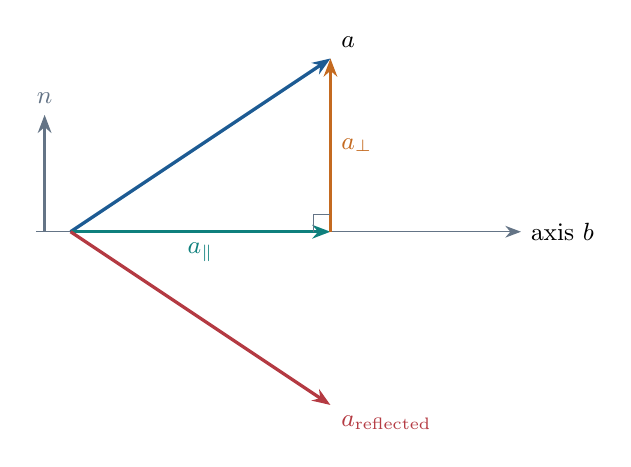
\begin{tikzpicture}[scale=1.1]
\draw[axis] (-.4,0)--(5.2,0) node[right]{axis $b$};
\draw[guide] (3,2)--(3,0);
\draw[vector] (0,0)--(3,2) node[above right]{$a$};
\draw[vector,manualteal] (0,0)--(3,0) node[midway,below]{$a_{\parallel}$};
\draw[vector,manualorange] (3,0)--(3,2) node[midway,right]{$a_{\perp}$};
\draw[vector,manualred] (0,0)--(3,-2) node[below right]{$a_\mathrm{reflected}$};
\draw[vector,manualmuted] (-.3,0)--(-.3,1.35) node[above]{$n$};
\draw[manualmuted] (2.8,0)--(2.8,.2)--(3,.2);
\end{tikzpicture}
\caption{Projection and rejection decompose a vector. Reflection across
the horizontal line reverses the normal component and retains the parallel
component.}
\label{fig:vector-components}
\end{figure}

\api{angle_to(other, tolerance)} returns an unsigned angle in radians
between zero and $\pi$, using a clamped cosine. Its degeneracy test compares
the product of the lengths to the square of the supplied tolerance.
\api{vector2::signed_angle_to(other, tolerance)} instead returns the
counterclockwise signed angle in $[-\pi,\pi]$, rejecting either individual
direction when it is too small. There is no signed 3D angle without an
additional orientation convention.

\begin{lstlisting}[language=C++]
const vector2<double> velocity{3.0, 2.0};
const auto along = velocity.projected_onto(vector2<double>{1.0, 0.0});
const auto across = velocity.rejected_from(vector2<double>{1.0, 0.0});
const auto bounced = velocity.reflected(vector2<double>{0.0, 1.0});
const double turn = vector2<double>::unit_x().signed_angle_to(velocity);
\end{lstlisting}

\section{Rotation about a 3D origin axis}

The free function \api{rotate(axis, angle, point)} rotates a
\api{point3<REAL>} about a direction through the Cartesian world origin.
The axis need not be normalized and the signed angle is in radians, following
the right-hand rule. An exactly zero axis throws \api{std::domain_error}.
Finite components, point coordinates, and angle are required for a finite
result. The function uses Rodrigues' formula:
\[
 R(p)=\cos\theta\,p+\sin\theta\,(\widehat a\times p)
 +(1-\cos\theta)(\widehat a\cdot p)\widehat a.
\]

For rotation about an axis through a different point $C$, explicitly shift
the position to the origin, rotate it, and shift it back:

\begin{lstlisting}[language=C++]
const point3<double> center{2.0, 1.0, 0.0};
const point3<double> position{3.0, 1.0, 0.0};
const vector3<double> offset = position - center;
const point3<double> relative{offset.x, offset.y, offset.z};
const auto rotated_relative = rotate(
    vector3<double>::unit_z(), std::numbers::pi / 2.0, relative);
const auto rotated = center + vector3<double>{rotated_relative};
\end{lstlisting}

\begin{figure}[htbp]
\centering
\begin{tikzpicture}[scale=1.05]
\draw[axis] (-.4,0)--(4.5,0) node[right]{$x$};
\draw[axis] (0,-.4)--(0,3.7) node[above]{$y$};
\draw[guide] (0,0) circle[radius=2.6];
\draw[vector] (0,0)--(2.6,0) node[below]{$P$};
\draw[vector,manualteal] (0,0)--(1.3,2.252) node[above right]{$R(P)$};
\draw[manualorange,thick,-{Latex}] (1,0) arc[start angle=0,end angle=60,radius=1];
\node[manualorange] at (1.25,.68) {$\theta$};
\node[point,label=below left:$O$] at (0,0) {};
\node[anchor=west,align=left] at (3.2,2.5) {axis $+z$\\out of the page};
\end{tikzpicture}
\caption{Positive rotation about $+z$ appears counterclockwise when viewed
from the positive-Z side. The public rotation call is for a 3D point.}
\end{figure}

\section{Rays and their native parameter}

Construct a ray with an origin, direction, and optional minimum direction
length. The \api{ray2} and \api{ray3} APIs have the same forms:

\begin{lstlisting}[language=C++]
ray2<double> ray_2d(point2<double>{1.0, 1.0},
                    vector2<double>{2.0, 0.5});
ray3<double> ray_3d(point3<double>{1.0, 1.0, 0.0},
                    vector3<double>{2.0, 0.5, 0.0});
const auto at_two = ray_3d.point_at(2.0);
const auto same_point = ray_3d.evaluate(2.0);
const auto unit_tangent = ray_3d.tangent();
\end{lstlisting}

The native parameterization is
\[
 r(s)=O+sD,\qquad s\geq0.
\]
Construction preserves $D$ exactly rather than normalizing it. A parameter
change $\Delta s$ therefore moves through a world distance
$|\Delta s|\,\lVert D\rVert$; $s$ is itself a distance only for a unit
direction. \api{point_at} and its alias \api{evaluate} evaluate the formula
even for a negative argument, but ray intersection and distance queries use
the forward half-line. \api{tangent()} returns the normalized positive
direction without changing the stored ray.

\begin{figure}[htbp]
\centering
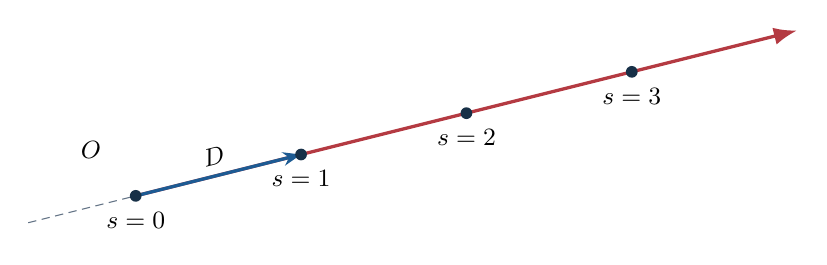
\begin{tikzpicture}[scale=1.05]
\draw[guide] (-1.3,-.325)--(0,0);
\draw[manualred,very thick,-{Latex}] (0,0)--(8,2);
\draw[vector] (0,0)--(2,.5) node[midway,above,sloped]{$D$};
\foreach \station/\rayx/\rayy in {0/0/0,1/2/.5,2/4/1,3/6/1.5}{
 \node[point,label=below:{$s=\station$}] at (\rayx,\rayy) {};
}
\node[anchor=east] at (-.3,.55) {$O$};
\end{tikzpicture}
\caption{Uniform increments in $s$ follow the unnormalized direction. The
dashed continuation behind the origin is outside the ray domain.}
\end{figure}

\api{origin()} and \api{direction()} return constant references;
\api{get_origin()} and \api{get_direction()} are equivalent getters.
Use \api{set_origin}, \api{set_direction}, or
\api{set_origin_and_direction} to edit the definition. The direction and
bulk setters validate before committing, leaving the ray unchanged when the
new direction is rejected. The constructor and these setters throw
\api{std::invalid_argument} when the direction is within the supplied
tolerance of zero. Origin setters also accept a same-world vector and copy
its components as coordinates.

\section{Circle and sphere surfaces}

\api{circle2(center, radius)} and \api{sphere3(center, radius)} require a
finite, strictly positive radius. Both expose \api{center()} and
\api{radius()}, with equivalent \api{get_center()} and \api{get_radius()}
forms. A circle remains a native 2D entity; a sphere is a 3D surface.

\subsection{A circle's angular coordinate}

For center $C$ and radius $R$, \api{circle2::point_at(u)} evaluates
\[
 C+R(\cos u,\sin u).
\]
The angle is in radians and increases counterclockwise from positive X.
\api{parameter_of(point, tolerance)} obtains $u\in[0,2\pi)$ by radial
projection, so the input need not lie on the circle. It throws
\api{std::domain_error} within the supplied center-distance tolerance and
\api{std::invalid_argument} for a negative tolerance.
\api{normal_at(point)} returns the normalized radial vector and rejects
the exactly central point.

\begin{figure}[htbp]
\centering
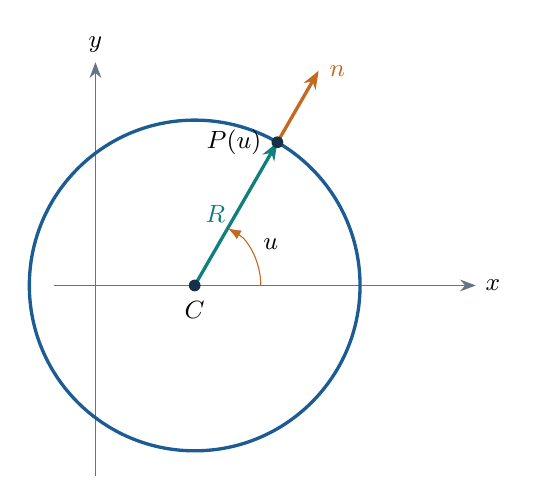
\begin{tikzpicture}[scale=1.05]
\draw[axis] (-.5,0)--(4.6,0) node[right]{$x$};
\draw[axis] (0,-2.3)--(0,2.7) node[above]{$y$};
\coordinate (C) at (1.2,0); \coordinate (P) at (2.2,1.732);
\draw[curve] (C) circle[radius=2];
\draw[vector,manualteal] (C)--(P) node[midway,left]{$R$};
\draw[vector,manualorange] (P)--(2.7,2.598) node[right]{$n$};
\draw[guide] (C)--(3.4,0);
\draw[manualorange,-{Latex}] (2,0) arc[start angle=0,end angle=60,radius=.8];
\node at (2.12,.5) {$u$};
\node[point,label=below:$C$] at (C) {};
\node[point,label=left:$P(u)$] at (P) {};
\end{tikzpicture}
\caption{A circle's parameter is an angle, while its outward normal is a
unit radial vector.}
\end{figure}

\begin{lstlisting}[language=C++]
circle2<double> boundary(point2<double>{1.0, 0.0}, 2.0);
const auto p = boundary.point_at(std::numbers::pi / 3.0);
const double u = boundary.parameter_of(p);
const auto outward = boundary.normal_at(p);
\end{lstlisting}

\subsection{Longitude and latitude on a sphere}

\api{sphere3::point_at(u, v)} evaluates
\[
 C+R(\cos v\cos u,\ \cos v\sin u,\ \sin v).
\]
The reported longitude lies in $[0,2\pi)$ and latitude in
$[-\pi/2,\pi/2]$. Longitude is not geometrically unique at the poles.
\api{parameters_of(point, tolerance)} obtains the pair by radial
projection, with the same center rejection and negative-tolerance exceptions
as the circle. \api{normal_at(point)} is the outward unit radial direction
and throws at the center.

\begin{figure}[htbp]
\centering
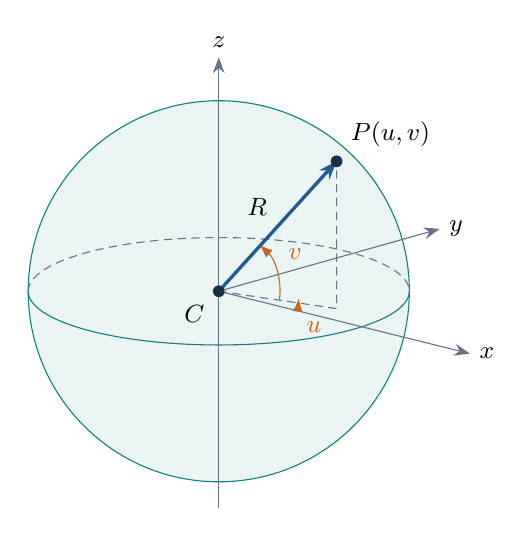
\begin{tikzpicture}[scale=1.1]
\draw[surface] (0,0) circle[radius=2.2];
\draw[guide] (-2.2,0) arc[start angle=180,end angle=0,x radius=2.2,y radius=.62];
\draw[manualteal] (-2.2,0) arc[start angle=180,end angle=360,x radius=2.2,y radius=.62];
\draw[axis] (0,-2.5)--(0,2.7) node[above]{$z$};
\draw[axis] (0,0)--(2.9,-.72) node[right]{$x$};
\draw[axis] (0,0)--(2.55,.72) node[right]{$y$};
\coordinate (P) at (1.36,1.50); \coordinate (Q) at (1.36,-.20);
\draw[vector] (0,0)--(P) node[midway,above left]{$R$};
\draw[guide] (0,0)--(Q)--(P);
\draw[manualorange,-{Latex}] (.7,-.10) arc[start angle=-8,end angle=48,radius=.72];
\node[manualorange] at (.88,.43) {$v$};
\draw[manualorange,-{Latex}] (.9,-.225) arc[start angle=-14,end angle=-5,radius=.93];
\node[manualorange] at (1.1,-.42) {$u$};
\node[point,label=above right:{$P(u,v)$}] at (P) {};
\node[point,label=below left:$C$] at (0,0) {};
\end{tikzpicture}
\caption{Sphere coordinates use longitude around the Z axis and latitude
above the XY plane. This is a schematic 3D view.}
\end{figure}

\begin{lstlisting}[language=C++]
sphere3<double> ball(point3<double>{0.0, 0.0, 0.0}, 2.0);
const auto surface_point = ball.point_at(
    std::numbers::pi / 4.0, std::numbers::pi / 6.0);
const auto [longitude, latitude] = ball.parameters_of(surface_point);
const auto normal = ball.normal_at(surface_point);
\end{lstlisting}

For either type, \api{set_center} preserves the radius,
\api{set_radius} validates the new radius, and
\api{set_center_and_radius} validates before updating either member. Failed
radius validation leaves the object unchanged. Center setters and the bulk
setter accept a same-world vector as a component source; assignment from
such a vector also replaces the center while preserving the radius.
Center-coordinate copying does not itself validate finiteness. Supply finite
geometric coordinates when a later operation requires a finite result.

\section{Planes: an orthonormal local frame}

A \api{plane3} stores a world-space parameter origin $O$, a unit normal
$\widehat n$, and orthonormal directions $\widehat u,\widehat v$ with
$\widehat u\times\widehat v=\widehat n$. Its creation forms are:

\begin{lstlisting}[language=C++]
const auto z = vector3<double>::unit_z();
plane3<double> hessian(z, 2.0);
plane3<double> positioned(point3<double>{0.0, 0.0, 2.0}, z);
plane3<double> oriented(point3<double>{0.0, 0.0, 2.0}, z,
                         vector3<double>::unit_x());
\end{lstlisting}

The Hessian form \api{plane3(normal, signed_distance, tolerance)} first
normalizes the supplied normal. Its equation is
$\widehat n\cdot x=d$, and its parameter origin is $d\widehat n$.
The distance is signed in world units; it is not scaled by the magnitude of
the original normal. A non-finite distance throws
\api{std::invalid_argument}.

The origin-and-normal form places $(u,v)=(0,0)$ at the given world point and
chooses a stable in-plane frame. The third form adds a preferred
\api{u_hint}: the constructor rejects its normal component and normalizes
what remains. The normal and accepted in-plane hint must exceed the supplied
tolerance, otherwise \api{std::domain_error} is thrown. Both forms retain
the supplied parameter origin rather than moving it to the Hessian closest
point.

\begin{figure}[htbp]
\centering
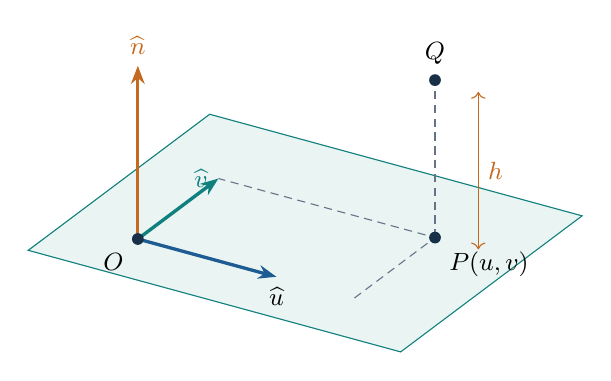
\begin{tikzpicture}[x={(1.1cm,-.30cm)},y={(.64cm,.48cm)},z={(0cm,1cm)}]
\fill[surface] (-.8,-.8,0)--(3.5,-.8,0)--(3.5,2.8,0)--(-.8,2.8,0)--cycle;
\coordinate (O) at (0,0,0); \coordinate (P) at (2.5,1.6,0);
\draw[vector] (O)--(1.6,0,0) node[below]{$\widehat u$};
\draw[vector,manualteal] (O)--(0,1.6,0) node[left]{$\widehat v$};
\draw[vector,manualorange] (O)--(0,0,2.2) node[above]{$\widehat n$};
\draw[guide] (2.5,0,0)--(P)--(0,1.6,0);
\draw[guide] (P)--(2.5,1.6,2);
\node[point,label=below left:$O$] at (O) {};
\node[point,label=below right:{$P(u,v)$}] at (P) {};
\node[point,label=above:$Q$] at (2.5,1.6,2) {};
\draw[manualorange,<->] (3,1.6,0)--(3,1.6,2) node[midway,right]{$h$};
\end{tikzpicture}
\caption{The orthonormal frame gives world-distance plane coordinates.
Orthogonal projection removes the signed height $h$ along the normal.}
\label{fig:plane-frame}
\end{figure}

\api{point_at(u, v)} evaluates $O+u\widehat u+v\widehat v$.
For any world point $Q$, \api{signed_distance_to(Q)} returns
$h=(Q-O)\cdot\widehat n$, \api{project(Q)} returns
$Q-h\widehat n$, and \api{parameters_of(Q)} returns
$((Q-O)\cdot\widehat u,(Q-O)\cdot\widehat v)$. Thus coordinates may be
recovered from an off-plane point without first calling \api{project}.
The member \api{project(point3)} is an orthogonal point projection within
the 3D world. The free \api{project(plane3, entity2)} is the separate,
explicit embedding operation.

\begin{lstlisting}[language=C++]
const point3<double> query{1.0, 3.0, 5.0};
const double height = oriented.signed_distance_to(query);
const auto foot = oriented.project(query);
const auto [u, v] = oriented.parameters_of(query);
const auto reconstructed = oriented.point_at(u, v);
\end{lstlisting}

\api{origin()}, \api{normal()}, \api{u_direction()}, and
\api{v_direction()} are constant-reference getters. Their
\api{get_...} forms are equivalent. Two further equivalent getters report
$\widehat n\cdot O$:
\begin{itemize}[leftmargin=*]
\item \api{signed_distance_from_origin()};
\item \api{get_signed_distance_from_origin()}.
\end{itemize}

\api{set_origin} moves the parameter origin and retains the frame.
\api{set_normal} retains the origin and generates a new stable frame;
\api{set_u_direction} retains the origin and normal and rebuilds the two
in-plane directions from a hint. \api{set_definition} has Hessian,
origin-and-normal, and origin-normal-hint forms matching construction. These
frame-changing setters build a complete candidate before committing it, so
a rejected normal or hint leaves the original plane unchanged. Origin-based
setters also accept a \api{vector3} whose components become coordinates.
The normal and in-plane basis directions remain read-only through getters.

\section{Reading the contracts consistently}

Coordinate access and simple arithmetic are deliberately lightweight. They
do not impose a universal finite-value check on every assignment. In
contrast, radius validation, direction degeneracy checks, frame construction,
NURBS definition validation, and record encoding have specific documented
checks. A zero vector is a valid stored vector but cannot define a unit
direction or plane normal. A point at a sphere or circle center is a valid
position but has no radial surface coordinate.

Point and vector CSV, whitespace, binary, and selected 3D tagged I/O members
are described with the complete output protocols later in this manual.
Those methods do not change the geometric distinction between positions and
displacements.

\chapter{Construction and shared ownership}
\label{chap:creators}

The public constructors create values. The allocation helpers in
\api{nurbspath/creators.hpp} create the corresponding values under
\api{std::shared_ptr} ownership. They retain the constructors' geometric
validation and exceptions. Both styles are useful: local calculations often
use values, while a collection with shared lifetime may use factory results.
The umbrella header includes these helpers.

\begin{lstlisting}[language=C++]
#include <nurbspath/config.hpp>
#include <nurbspath/nurbspath.hpp>

using namespace nurbspath;
point3<double> value{1.0, 2.0, 3.0};
auto shared = make_point3<double>(1.0, 2.0, 3.0);
const double separation = distance(value, *shared);
\end{lstlisting}

The suffix identifies the Cartesian world. A 2D factory never silently
allocates a 3D entity. Calls below use \api{double}; replacing it with
another standard floating-point type changes the scalar type throughout.
Allocation can throw \api{std::bad_alloc} in addition to the validation
exceptions noted for each entity.

\section{Point and vector factory catalogue}

\begin{longtable}{@{}p{.43\linewidth}p{.52\linewidth}@{}}
\caption{All point and vector allocation families. Each result is a shared
pointer to the type named after \api{make_}.}\\
\toprule
Call arguments after the template & Created value \\
\midrule
\endfirsthead
\toprule Call arguments after the template & Created value \\
\midrule
\endhead
\api{make_point2<REAL>()} & The 2D origin. \\
\api{make_point2<REAL>(x, y)} & A 2D position with the supplied coordinates. \\
\api{make_point3<REAL>()} & The 3D origin. \\
\api{make_point3<REAL>(x, y, z)} & A 3D position with the supplied coordinates. \\
\api{make_vector2<REAL>()} & The 2D zero vector. \\
\api{make_vector2<REAL>(x, y)} & The supplied 2D components. \\
\api{make_vector2<REAL>(point)} & Coordinates copied from a \api{point2}. \\
\api{make_vector2<REAL>(circle)} & Center coordinates copied from a \api{circle2}. \\
\api{make_vector2<REAL>(ray)} & Origin coordinates copied from a \api{ray2}. \\
\api{make_vector3<REAL>()} & The 3D zero vector. \\
\api{make_vector3<REAL>(x, y, z)} & The supplied 3D components. \\
\api{make_vector3<REAL>(point)} & Coordinates copied from a \api{point3}. \\
\api{make_vector3<REAL>(sphere)} & Center coordinates copied from a \api{sphere3}. \\
\api{make_vector3<REAL>(plane)} & Parameter-origin coordinates copied from a \api{plane3}. \\
\api{make_vector3<REAL>(ray)} & Origin coordinates copied from a \api{ray3}. \\
\bottomrule
\end{longtable}

The entity-to-vector factories perform the same explicit component copy as
the constructors in Chapter~\ref{chap:entities}. To allocate a copy of a
ray direction, obtain \api{ray.direction()} and use its components, or use
\api{std::make_shared<vector3<double>>(ray.direction())}.

\section{Ray, circle, and sphere creation}

The origin-and-direction helpers are \api{make_ray2} and \api{make_ray3}.
The two-point helpers are \api{make_ray2_from_points} and
\api{make_ray3_from_points}.
The first takes \api{(origin, direction, tolerance)}; the second takes
\api{(origin, through_point, tolerance)}. Tolerance is optional and defaults
to \api{vector2<REAL>::default_tolerance()} or its 3D counterpart.
The point-based helper uses \api{through_point - origin} directly, with
no normalization. The through point is therefore at native parameter $s=1$.

\begin{lstlisting}[language=C++]
const point2<double> a2{1.0, 1.0};
const point2<double> b2{3.0, 2.0};
auto ray_a = make_ray2<double>(a2, b2 - a2);
auto ray_b = make_ray2_from_points<double>(a2, b2);
auto circle = make_circle2<double>(point2<double>{0.0, 0.0}, 2.0);

const point3<double> a3{1.0, 1.0, 0.0};
const point3<double> b3{3.0, 2.0, 1.0};
auto ray_c = make_ray3<double>(a3, b3 - a3);
auto ray_d = make_ray3_from_points<double>(a3, b3);
auto sphere = make_sphere3<double>(point3<double>{0.0, 0.0, 0.0}, 2.0);
\end{lstlisting}

A direction or point separation within the ray tolerance throws
\api{std::invalid_argument}. \api{make_circle2(center, radius)} and
\api{make_sphere3(center, radius)} require finite, positive radii and throw
\api{std::invalid_argument} otherwise. These are the complete circle and
sphere factory families; they do not infer a circle or sphere from several
boundary points.

\section{Five ways to allocate a plane}

The three \api{make_plane3} overloads mirror the three constructors:

\begin{enumerate}[leftmargin=*]
\item \api{(normal, signed_distance, tolerance)} uses Hessian normal form.
\item \api{(origin, normal, tolerance)} chooses a stable in-plane frame.
\item \api{(origin, normal, u_hint, tolerance)} sets the preferred positive-u
direction by in-plane projection.
\end{enumerate}

Two named helpers derive an oriented frame from construction geometry:
\begin{itemize}[leftmargin=*]
\item \api{make_plane3_from_u_direction} takes \api{origin},
\api{u_direction}, \api{plane_point}, and optional \api{tolerance}.
\item \api{make_plane3_from_points} takes \api{origin}, \api{u_point},
\api{plane_point}, and optional \api{tolerance}; it uses
\api{u_point - origin} as its positive-u direction.
\end{itemize}
The third point determines the positive-v side by rejection from that axis:
\[
 \widehat u=\frac{U}{\lVert U\rVert},\quad
 V=(P-O)-((P-O)\cdot\widehat u)\widehat u,\quad
 \widehat v=\frac{V}{\lVert V\rVert},\quad
 \widehat n=\widehat u\times\widehat v.
\]
All five helpers accept the optional vector tolerance. A short normal,
u-direction, or rejected v-component causes a \api{std::domain_error}
exception. A non-finite Hessian distance causes \api{std::invalid_argument}.

\begin{lstlisting}[language=C++]
const point3<double> origin{1.0, 2.0, 3.0};
const point3<double> u_point{3.0, 2.0, 3.0};
const point3<double> plane_point{2.0, 4.0, 3.0};
auto hessian = make_plane3<double>(vector3<double>{0.0, 0.0, 2.0}, 3.0);
auto from_normal = make_plane3<double>(origin, vector3<double>::unit_z());
auto with_hint = make_plane3<double>(
    origin, vector3<double>::unit_z(), vector3<double>::unit_x());
auto from_direction = make_plane3_from_u_direction<double>(
    origin, vector3<double>{2.0, 0.0, 0.0}, plane_point);
auto from_points = make_plane3_from_points<double>(origin, u_point, plane_point);
\end{lstlisting}

\begin{figure}[htbp]
\centering
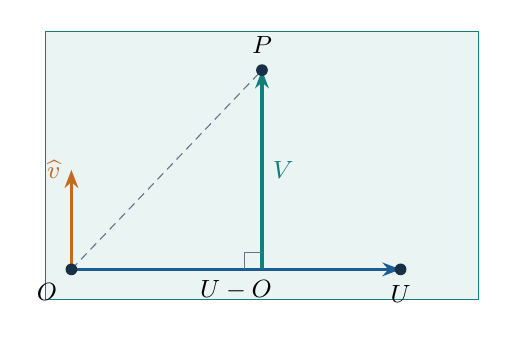
\begin{tikzpicture}[scale=1.1]
\fill[surface] (-.3,-.35)--(4.7,-.35)--(4.7,2.75)--(-.3,2.75)--cycle;
\coordinate (O) at (0,0); \coordinate (U) at (3.8,0);
\coordinate (P) at (2.2,2.3); \coordinate (H) at (2.2,0);
\draw[vector] (O)--(U) node[midway,below]{$U-O$};
\draw[guide] (O)--(P);
\draw[guide] (P)--(H);
\draw[vector,manualteal] (H)--(P) node[midway,right]{$V$};
\draw[vector,manualorange] (O)--(0,1.15) node[left]{$\widehat v$};
\node[point,label=below left:$O$] at (O) {};
\node[point,label=below:$U$] at (U) {};
\node[point,label=above:$P$] at (P) {};
\draw[manualmuted] (2,.0)--(2,.2)--(2.2,.2);
\end{tikzpicture}
\caption{Three-point plane construction viewed in the plane itself. The
third point chooses the positive-v side; its along-u component is discarded
when the frame is built.}
\end{figure}

Moving the third point across the u-axis reverses both $\widehat v$ and
$\widehat n$. Three collinear points do not determine a plane through this
interface. A supplied normal or u-direction need not have unit length.

\section{Ordinary spline constructors and factories}

The following catalogue applies independently to \api{nurbs_spline2} and
\api{nurbs_spline3}. Write \api{S} for either type,
\api{P} for its same-world point type, \api{A} for the corresponding
array-backed type, \api{p} for the degree, \api{n} for the control-point
count, and \api{tol} for the positive definition tolerance. The factories
\api{make_nurbs_spline2} and \api{make_nurbs_spline3} return
\api{std::shared_ptr<S>}.

\begin{table}[htbp]
\centering
\caption{Complete ordinary-spline construction families. Optional brackets
describe permitted omitted arguments, not C++ syntax.}
\begin{tabularx}{\linewidth}{@{}p{.52\linewidth}Y@{}}
\toprule
Argument sequence & Availability and behavior \\
\midrule
\api{start, end, n, p} & Constructor and factory; standard open definition. \\
\api{start, end, n, p, tol} & Constructor and factory; explicit tolerance. \\
\api{start, end, n, p, closed [, tol]} & Constructor and factory; explicit Boolean closure request. \\
\api{points, weights, knots, p [, tol]} & Constructor and factory with \api{std::vector} collections. \\
\api{points, weights, knots, p, closed [, tol]} & Constructor and factory with vector collections and a closure request. \\
\api{points, weights, knots, p [, tol]} & Factory also accepts point/scalar \api{std::valarray} collections. \\
\api{points, weights, knots, p, closed [, tol]} & Factory also accepts valarrays and a closure request. \\
\api{array_spline} & Explicit constructor and factory; copy from corresponding \api{A}. \\
\bottomrule
\end{tabularx}
\end{table}

The omitted spline tolerance is
\api{64 * std::numeric_limits<REAL>::epsilon()}.
The standard constructor places $n$ control points uniformly from start to
end with unit weights and open-clamped knots over
$[0,\operatorname{distance}(\mathrm{start},\mathrm{end})]$. It creates a
straight curve, with a positive domain extent required by validation.
The explicit-tolerance fifth argument is a scalar; the closure overload
requires an actual \api{bool}, avoiding accidental interpretation of a
tolerance as a closure flag.

\begin{lstlisting}[language=C++]
const point2<double> start{0.0, 0.0};
const point2<double> end{4.0, 0.0};
nurbs_spline2<double> line(start, end, 5, 2);
auto shared_line = make_nurbs_spline2<double>(start, end, 5, 2);
auto explicit_tolerance = make_nurbs_spline2<double>(start, end, 5, 2, 1e-10);
auto explicit_open = make_nurbs_spline2<double>(start, end, 5, 2, false, 1e-10);
\end{lstlisting}

Complete definitions supply every control point, positive weight, and knot.
For $n$ control points and degree $p$, the knot count is $n+p+1$, with
$0<p<n$, nondecreasing finite knots, and a nonempty active domain. The
standard and complete-definition families have matching validation contracts;
the full mathematical requirements are in Chapter~\ref{chap:splines}.

\begin{lstlisting}[language=C++]
std::vector<point3<double>> points{
    {0.0, 0.0, 0.0}, {1.0, 2.0, 0.5}, {3.0, 0.0, 1.0}};
std::vector<double> weights{1.0, 1.0, 1.0};
std::vector<double> knots{0.0, 0.0, 0.0, 2.0, 2.0, 2.0};
nurbs_spline3<double> value_curve(points, weights, knots, 2);
auto shared_curve = make_nurbs_spline3<double>(points, weights, knots, 2);

std::valarray<point3<double>> array_points{points.data(), points.size()};
std::valarray<double> array_weights{weights.data(), weights.size()};
std::valarray<double> array_knots{knots.data(), knots.size()};
auto copied_arrays = make_nurbs_spline3<double>(
    array_points, array_weights, array_knots, 2, false);
\end{lstlisting}

The ordinary constructors take vectors. The ordinary factories additionally
accept const, mutable, lvalue, or rvalue valarrays of same-world points plus
scalar valarrays; they copy them in index order into ordinary vector storage.
Brace-list calls remain available through the vector overloads.

\subsection{Closure describes a seam}

A \api{closed = true} request requires coincident evaluated endpoints of
the active domain within the spline tolerance. It does not append a control
point or synthesize a loop from a straight start/end construction. Use a
complete definition or closed interpolation samples to create a useful closed
shape.

\begin{lstlisting}[language=C++]
auto closed_polygon = make_nurbs_spline2<double>(
    std::vector<point2<double>>{
        {0.0, 0.0}, {2.0, 0.0}, {1.0, 1.5}, {0.0, 0.0}},
    std::vector<double>{1.0, 1.0, 1.0, 1.0},
    std::vector<double>{0.0, 0.0, 1.0, 2.0, 3.0, 3.0},
    1, true);
\end{lstlisting}

\begin{figure}[htbp]
\centering
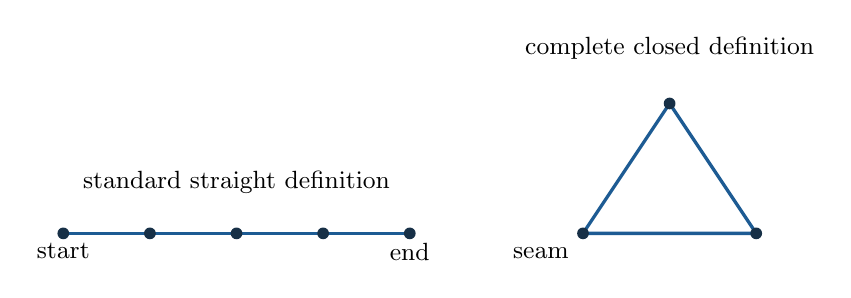
\begin{tikzpicture}[scale=1.1]
\begin{scope}
\draw[curve] (0,0)--(4,0);
\foreach \x in {0,1,2,3,4}{\node[point] at (\x,0) {};}
\node[below] at (0,0) {start}; \node[below] at (4,0) {end};
\node[above] at (2,.35) {standard straight definition};
\end{scope}
\begin{scope}[shift={(6,0)}]
\draw[curve] (0,0)--(2,0)--(1,1.5)--cycle;
\node[point,label=below left:seam] at (0,0) {};
\node[point] at (2,0) {}; \node[point] at (1,1.5) {};
\node[above] at (1,1.9) {complete closed definition};
\end{scope}
\end{tikzpicture}
\caption{The standard factory places control points along a segment. A
closed flag validates a seam; the supplied definition determines the shape.}
\end{figure}

\section{Array-backed spline construction}

\api{nurbs_arr_spline2} and \api{nurbs_arr_spline3} are separate classes,
not derived ordinary splines. Their public \api{std::valarray<REAL> parameters}
contains point-major control coordinates, then all weights, then all knots.
The degree, tolerance, and closure state are stored separately. This layout
is useful when an optimizer must copy or replace the entire scalar state.
The conversion operations retain the Cartesian world.

For dimension $d$, $n$ controls, and degree $p$, the flattened length is
$(d+2)n+p+1$. In 2D it is
\[
 [x_0,y_0,\ldots,x_{n-1},y_{n-1},
   w_0,\ldots,w_{n-1},k_0,\ldots,k_{n+p}],
\]
and in 3D each point contributes X/Y/Z coordinates.

\begin{table}[htbp]
\centering
\caption{Complete array-backed construction families, for both dimensions.
Direct constructors and shared-pointer factories support the same families.}
\begin{tabularx}{\linewidth}{@{}p{.57\linewidth}Y@{}}
\toprule
Argument sequence & Created definition \\
\midrule
\api{start, end, n, p} & Standard open straight curve. \\
\api{start, end, n, p, tol} & Standard curve with explicit tolerance. \\
\api{start, end, n, p, closed [, tol]} & Standard curve with a Boolean closure request. \\
\api{parameters, p [, tol]} & Open definition from flattened scalar valarray. \\
\api{parameters, p, closed [, tol]} & Flattened definition with a Boolean closure request. \\
\api{points, weights, knots, p [, tol]} & Open definition from component vectors. \\
\api{points, weights, knots, p, closed [, tol]} & Component-vector definition with a Boolean closure request. \\
\api{ordinary_spline} & Independent copy from corresponding ordinary spline. \\
\bottomrule
\end{tabularx}
\end{table}

The matching factory names are \api{make_nurbs_arr_spline2} and
\api{make_nurbs_arr_spline3}.
The component collection overloads take \api{std::vector}s; a flattened
overload takes one scalar \api{std::valarray}. The point-valarray overloads
listed for ordinary factories are not separate array-backed factory
overloads. The constructors and factories reject malformed array shapes
before indexing the data.

\begin{lstlisting}[language=C++]
std::valarray<double> parameters{
    0.0, 0.0,  1.0, 2.0,  3.0, 0.0,  // three 2D controls
    1.0, 1.0, 1.0,                    // weights
    0.0, 0.0, 0.0, 2.0, 2.0, 2.0};  // quadratic knots
nurbs_arr_spline2<double> array_curve(parameters, 2);
auto shared_array = make_nurbs_arr_spline2<double>(parameters, 2, false);
\end{lstlisting}

\section{Conversions and definition updates}

Conversions between the ordinary and array-backed representations are
explicit, copying control points, weights, knots, degree, tolerance, closure,
and the native parameter domain. They allocate independent storage:

\begin{lstlisting}[language=C++]
auto ordinary = make_nurbs_spline2<double>(*shared_array);
auto flattened = make_nurbs_arr_spline2<double>(*ordinary);
nurbs_spline2<double> ordinary_value(*flattened);
nurbs_arr_spline2<double> array_value(ordinary_value);
\end{lstlisting}

The same calls are available for the 3D pair. These conversions never add,
remove, or reinterpret a coordinate dimension. Converting an array-backed
definition validates its current public storage; a malformed state throws
rather than yielding a partially constructed spline.

Ordinary spline definition storage is private. Checked setters preserve the
degree, validate a complete proposed state, and refresh cached endpoints only
after success. A failed update leaves the spline unchanged. The array-backed
alternatives expose scalar storage and derive endpoint state when needed;
direct edits must be followed by \api{validate()} or a checked geometry
operation. Chapter~\ref{chap:splines} gives the complete editing and
evaluation APIs for both representations.

\chapter{NURBS curves and interpolation}
\label{chap:splines}

\section{One curve definition, two separate worlds}

The ordinary curve types are \api{nurbs_spline2<REAL>} and
\api{nurbs_spline3<REAL>}. Their coordinate storage is private, their definition
is checked at construction and after each setter, and their active-domain
endpoints are cached. The corresponding \api{nurbs_arr_spline2<REAL>} and
\api{nurbs_arr_spline3<REAL>} types provide a different storage contract: a
public, flattened \api{std::valarray<REAL>} that an optimizer can edit directly.
All four types describe rational B-spline curves and provide position,
derivative, tangent, curvature, length, and interpolation operations.

The suffix is part of the geometry contract. A 2D curve evaluates to
\api{point2<REAL>} and differentiates to \api{vector2<REAL>}; a 3D curve uses
the corresponding 3D types. Constructing an array-backed curve from an ordinary
curve, or converting it back, preserves that suffix. Embedding a 2D curve into
3D is an explicit \api{project(plane, spline)} operation, described in
Chapter~\ref{chap:entities}.

For a curve with $C$ control points, degree $p$, weights $w_i$, and knots $K_j$,
the complete definition satisfies
\begin{equation}
 C>p\geq1,\qquad \#w=C,\qquad \#K=C+p+1,
 \qquad w_i>0,\qquad K_j\leq K_{j+1}.
\end{equation}
Coordinates, weights, knots, and the strictly positive definition tolerance
must be finite. The knot domain used by the curve is
\begin{equation}
\boxed{\quad s\in[K_p,K_C]=[\api{s_min()},\api{s_max()}]\quad}
\label{eq:spline-domain}
\end{equation}
and must have positive length. It is the \emph{active} domain; the first and
last values in the stored knot vector need not be its bounds.

\begin{manualnote}[Native parameters]
The parameter is named $s$, but a general NURBS definition does not make $s$
equal to distance traveled. Keep the native knot units when passing $s$ to
evaluation, intersections, distances, or derivative functions. Interpolation
preserves the supplied station values, including a nonzero first station.
\end{manualnote}

\section{Construction from a complete definition}
\label{sec:spline-definition}

The following fragment establishes a running example in the native 2D world.
It uses five control points, cubic basis functions, nonunit weights, and a
native domain of $[0,5]$. Code fragments in this chapter use the umbrella header
\api{<nurbspath/nurbspath.hpp>}; standard-library facilities need their usual
headers. The namespace alias \api{np} below is used throughout the chapter.

\begin{lstlisting}[language=C++,caption={A complete ordinary 2D curve definition.}]
namespace np = nurbspath;
using real = double;
using point = np::point2<real>;

const std::vector<point> controls{
    {0, 0}, {1, 2}, {2, -1}, {3, 2}, {4, 0}};
const std::vector<real> weights{1, 1, 0.7, 1.5, 1};
const std::vector<real> knots{0, 0, 0, 0, 2, 5, 5, 5, 5};

np::nurbs_spline2<real> curve(
    controls, weights, knots, 3, false, 1e-10);
const point start = curve.get_start();
const point end = curve.get_end();
const point middle = curve.point_at(2.5);
\end{lstlisting}

\begin{figure}[tbp]
\centering
\begin{tikzpicture}
\begin{axis}[
 width=.91\linewidth,height=6.2cm,axis equal image,
 axis lines=left,xlabel={$x$},ylabel={$y$},
 xmin=-.2,xmax=4.3,ymin=-1.65,ymax=2.6,clip=false,
 grid=major,grid style={manualmuted!15},
 legend style={draw=none,fill=white,font=\small,
   at={(.5,-.22)},anchor=north},legend columns=1]
\addplot[manualmuted,dashed,mark=*,mark size=2pt]
 table[x=x,y=y]{pictures/spline_controls.dat};
\addlegendentry{control polygon}
\addplot[manualblue,very thick,no marks]
 table[x=x,y=y]{pictures/spline_curve.dat};
\addlegendentry{evaluated rational curve}
\node[anchor=north west,font=\small] at (axis cs:0,-.1) {$P_0$, $w_0=1$};
\node[anchor=south,font=\small] at (axis cs:1,2) {$P_1$, $w_1=1$};
\node[anchor=north,font=\small] at (axis cs:2,-1.12) {$P_2$, $w_2=0.7$};
\node[anchor=south,font=\small] at (axis cs:3,2) {$P_3$, $w_3=1.5$};
\node[anchor=north east,font=\small] at (axis cs:4,-.1) {$P_4$, $w_4=1$};
\end{axis}
\end{tikzpicture}
\caption{Control points steer the curve; they are generally not samples on
it. The blue path is evaluated by the library. The clamped endpoint blocks in
this example make the evaluated endpoints coincide with $P_0$ and $P_4$.}
\label{fig:spline-controls}
\end{figure}

The complete-definition constructors accept three \api{std::vector}s followed
by the degree. Omitting the closure argument constructs an open curve; an
optional tolerance follows the degree in that overload. Supplying
\api{closed} before the tolerance enables the seam requirement. In 3D, replace
\api{point2} and \api{nurbs_spline2} with their 3D counterparts. There is no
default empty spline object: construction establishes a usable definition.

An open curve is allowed to have coincident endpoints. A closed curve requires
that coincidence, but does not by itself guarantee a smooth seam, matching
tangent vectors, matching curvature, or a periodic knot representation. For
the ordinary definition check, endpoint separation must not exceed
$16\,\tau\,\max(1,|\hbox{control coordinates}|)$, where $\tau$ is the definition
tolerance. Closed interpolation also checks its first and last input samples
against the supplied tolerance before solving.

The getter families \api{get_control_points()}, \api{get_weights()}, and
\api{get_knots()} return constant references for ordinary splines.
\api{get_control_point(i)}, \api{get_weight(i)}, and \api{get_knot(i)} select
individual values; an invalid index throws \api{std::out_of_range}.
\api{degree()}, \api{tolerance()}, and \api{is_closed()} report metadata.
\api{get_start()} and \api{get_end()} return constant references to evaluated,
cached endpoints, not editable definition fields.

\subsection{Starting with a standard straight curve}

When only endpoints and a number of controls are known, the standard
constructor lays the control points uniformly along the segment using
\api{lerp}, assigns unit weights, and builds standard open-clamped knots. Its
native domain is $[0,\operatorname{distance}(\mathrm{start},\mathrm{end})]$.
The degree must be positive and smaller than the requested control count.
The endpoints must define a finite, positive domain length.

\begin{lstlisting}[language=C++,caption={Standard construction and knot replacement.}]
np::nurbs_spline3<real> straight(
    np::point3<real>{0, 0, 0},
    np::point3<real>{4, 0, 3}, 6, 3);
// Native domain is initially [0, 5].
straight.set_standard_knots(10.0, 20.0);
// Explicit-tolerance overload, without a closure argument:
np::nurbs_spline2<real> straight2(
    point{0, 0}, point{4, 0}, 5, 2, 1e-10);
straight2.set_standard_knots(8.0);  // Domain [0, 8].
\end{lstlisting}

\api{set_standard_knots(s_end)} uses $[0,s_\mathrm{end}]$.
\api{set_standard_knots(s_start,s_end)} uses the stated bounds. Both repeat
each endpoint $p+1$ times and distribute any simple interior knots uniformly.
If $C=p+1$, the two endpoint blocks form the entire knot vector. The generated
spans must remain distinct and have finite positive lengths with finite
reciprocals in \api{REAL}. Invalid domains or numerically unusable spans are
rejected before the curve changes.

Replacing standard knots can change the distribution of points along an
existing curve. If the intent is only to rescale its parameter, apply one
affine transformation to \emph{every} old knot and pass the complete result
to \api{set_knots}; this preserves the geometric locus while changing its
native $s$ values and derivative scale. A closure flag on the straight
constructor still requires the ordinary endpoint check; it does not invent a
loop between two different endpoints.

\begin{figure}[tbp]
\centering
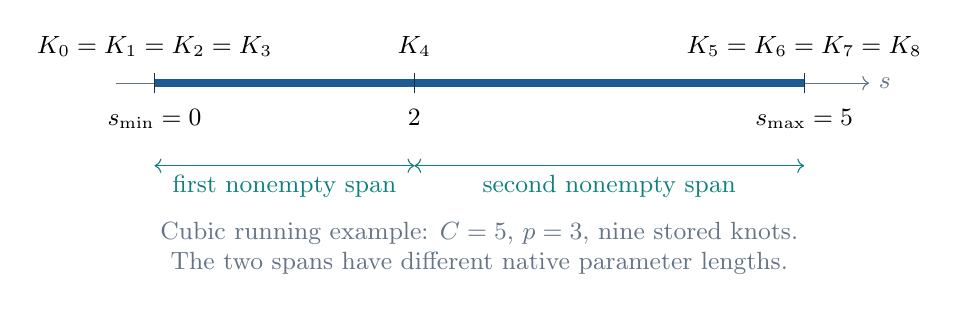
\begin{tikzpicture}[x=1.65cm,y=1cm,font=\small]
\draw[->,manualmuted] (-.3,0)--(5.5,0) node[right] {$s$};
\draw[manualblue,line width=3pt] (0,0)--(5,0);
\foreach \x/\lab in {0/{K_0=K_1=K_2=K_3},2/{K_4},5/{K_5=K_6=K_7=K_8}}{
 \draw[manualink] (\x,-.13)--(\x,.13);
 \node[above=6pt] at (\x,0) {$\lab$};}
\node[below=6pt] at (0,0) {$s_{\min}=0$};
\node[below=6pt] at (2,0) {$2$};
\node[below=6pt] at (5,0) {$s_{\max}=5$};
\draw[<->,manualteal] (0,-1.05)--(2,-1.05)
 node[midway,below] {first nonempty span};
\draw[<->,manualteal] (2,-1.05)--(5,-1.05)
 node[midway,below] {second nonempty span};
\node[align=center,text=manualmuted] at (2.5,-2.1)
 {Cubic running example: $C=5$, $p=3$, nine stored knots.\\
 The two spans have different native parameter lengths.};
\end{tikzpicture}
\caption{Stored knots and the active domain. Endpoint multiplicities describe
clamping; they are not extra finite intervals to sample.}
\label{fig:spline-knots}
\end{figure}

\section{Weights and exact conic geometry}

For basis functions $N_{i,p}$, a rational curve is
\begin{equation}
 \mathbf C(s)=\frac{\sum_{i=0}^{C-1}N_{i,p}(s)w_i\mathbf P_i}
                         {\sum_{i=0}^{C-1}N_{i,p}(s)w_i}.
\label{eq:rational-curve}
\end{equation}
The library evaluates only the nonzero basis functions in the selected knot
span. With positive weights, a control point with a larger relative weight
has more influence where its basis function is nonzero. Uniformly multiplying
the weights leaves the mathematical quotient unchanged, but a very small
common scale can trigger the implementation's near-zero homogeneous-weight
check. In particular, positivity alone is not a guarantee that every
arbitrarily scaled floating-point definition can be evaluated.

A rational quadratic represents a quarter of the unit circle exactly in real
arithmetic. It uses three controls, with the corner control carrying weight
$1/\sqrt2$. The native parameter below is $s\in[0,1]$; it is neither the circle
angle $u$ nor the traveled arc length.

\begin{lstlisting}[language=C++,caption={An exact rational quadratic quarter circle.}]
np::nurbs_spline2<real> quarter(
    std::vector<point>{{1, 0}, {1, 1}, {0, 1}},
    std::vector<real>{1, std::sqrt(0.5), 1},
    std::vector<real>{0, 0, 0, 1, 1, 1}, 2);
const point diagonal = quarter.evaluate(0.5);
const real quarter_curvature = quarter.curvature(0.5);
const auto rational_third = quarter.third_derivative(0.5);
\end{lstlisting}

\begin{figure}[tbp]
\centering
\begin{tikzpicture}
\begin{axis}[
 width=.7\linewidth,height=6.2cm,axis equal image,
 axis lines=left,xlabel={$x$},ylabel={$y$},
 xmin=-.12,xmax=1.25,ymin=-.12,ymax=1.3,
 xtick={0,.5,1},ytick={0,.5,1},grid=major,
 grid style={manualmuted!15}]
\addplot[manualmuted,dashed,mark=*,mark size=2pt]
 coordinates {(1,0) (1,1) (0,1)};
\addplot[manualblue,very thick,no marks]
 table[x=x,y=y]{pictures/rational_circle.dat};
\draw[manualteal,->] (axis cs:0,0)--(axis cs:.7071,.7071);
\addplot[only marks,manualorange,mark=*,mark size=2.5pt]
 coordinates {(.7071,.7071)};
\node[anchor=south west,font=\small] at (axis cs:.72,.73)
 {$s=\frac12$};
\node[anchor=south east,font=\small] at (axis cs:1,1)
 {$w_1=1/\sqrt2$};
\node[anchor=north,font=\small] at (axis cs:.4,.18) {$r=1$};
\end{axis}
\end{tikzpicture}
\caption{A quadratic rational curve lies on the unit circle, even though its
control polygon follows the two sides of a square. Its curvature is one in
inverse world units. The plotted blue points are library evaluations.}
\label{fig:rational-circle}
\end{figure}

Rounded output at the midpoint is
\begin{lstlisting}[caption={Rounded numerical preview; scientific precision is four decimals.}]
position: 7.0711e-01  7.0711e-01
curvature: 1.0000e+00
\end{lstlisting}
Although the homogeneous numerator and denominator have degree two within a
span, their quotient can have a nonzero third derivative. Calling
\api{third_derivative} on this quadratic is therefore meaningful; setting it
to zero solely because $p=2$ would be incorrect.

\section{Evaluation and analytic differential geometry}
\label{sec:spline-derivatives}

\api{evaluate(s)} and \api{point_at(s)} are equivalent position calls.
\api{derivatives_at(s)} computes position, first derivative, and second
derivative together. The result is \api{spline_derivatives2<REAL>} or
\api{spline_derivatives3<REAL>}, with members \api{point}, \api{first}, and
\api{second}. Separate calls are available as \api{first_derivative(s)},
\api{second_derivative(s)}, and \api{third_derivative(s)}.

\begin{lstlisting}[language=C++,caption={Position, derivatives, tangent, and curvature.}]
const real query_s = 2.5;
const auto jet = curve.derivatives_at(query_s);
const auto velocity = jet.first;
const auto acceleration = jet.second;
const auto third = curve.third_derivative(query_s);
const auto unit_tangent = curve.tangent(query_s);
const real curvature = curve.curvature(query_s);
// A consumer chooses how long a derivative arrow should appear:
const point arrow_tip = jet.point + 0.25 * velocity;
\end{lstlisting}

Let $\mathbf A^{(k)}=\sum_i N_{i,p}^{(k)}w_i\mathbf P_i$ and
$W^{(k)}=\sum_i N_{i,p}^{(k)}w_i$. Analytic differentiation is performed in
homogeneous form and then converted with the quotient recurrence
\begin{align}
\mathbf C^{(0)}&=\mathbf A^{(0)}/W^{(0)},\\
\mathbf C^{(r)}&=\frac{1}{W^{(0)}}\left(
 \mathbf A^{(r)}-\sum_{j=1}^{r}\binom rj
 W^{(j)}\mathbf C^{(r-j)}\right),\qquad r=1,2,3.
\label{eq:spline-quotient}
\end{align}
Homogeneous derivatives above the degree are zero, while the quotient
recurrence continues through the requested order. These are analytic basis
derivatives, rather than finite differences between neighboring points.

The derivatives are with respect to the native $s$. If $s$ has units of length,
the first derivative is dimensionless, the second has inverse-length units,
and the third has inverse-square-length units. If $s$ is dimensionless,
all three retain world-length units. More generally,
$\mathbf C^{(r)}$ has units of world length divided by parameter units to
power $r$. Scaling a derivative arrow for a diagram does not change these
API meanings.

\begin{figure}[tbp]
\centering
\begin{tikzpicture}
\begin{axis}[
 width=.47\linewidth,height=5.5cm,axis lines=left,
 xlabel={$s$},ylabel={first derivative},xmin=0,xmax=5,
 grid=major,grid style={manualmuted!15},
 legend style={draw=none,font=\small},legend pos=north east]
\addplot[manualblue,thick] table[x=s,y=dx]{pictures/spline_curve.dat};
\addlegendentry{$C'_x$}
\addplot[manualorange,thick] table[x=s,y=dy]{pictures/spline_curve.dat};
\addlegendentry{$C'_y$}
\end{axis}
\end{tikzpicture}\hfill
\begin{tikzpicture}
\begin{axis}[
 width=.47\linewidth,height=5.5cm,axis lines=left,
 xlabel={$s$},ylabel={$\kappa(s)$},xmin=0,xmax=5,
 grid=major,grid style={manualmuted!15}]
\addplot[manualteal,thick] table[x=s,y=curvature]{pictures/spline_curve.dat};
\end{axis}
\end{tikzpicture}
\caption{Analytic first-derivative components and curvature for the running
cubic curve. Speed and turning vary through the native domain. The plotted
values come from \api{first_derivative} and \api{curvature}.}
\label{fig:spline-differential}
\end{figure}

\subsection{Tangent and curvature contracts}

\api{tangent(s,tolerance)} normalizes the first derivative and throws
\api{std::domain_error} when its length is too small. Its default threshold
is the matching vector type's \api{default_tolerance()}. This is a derivative
length threshold; it is distinct from the spline definition tolerance and
from the world-distance tolerances used by geometric queries.

\api{curvature(s,tangent_tolerance)} returns an unsigned magnitude:
\begin{equation}
 \kappa_2=\frac{|\mathbf C'\mathbin{\times}\mathbf C''|}
                  {\|\mathbf C'\|^3},\qquad
 \kappa_3=\frac{\|\mathbf C'\mathbin{\times}\mathbf C''\|}
                  {\|\mathbf C'\|^3}.
\end{equation}
The 2D cross product in this formula is a scalar. Curvature has inverse
world-length units and is independent of regular reparameterization while
the required arithmetic remains representable. It does not encode the sign
of left or right turning. The threshold must be finite and nonnegative;
an invalid threshold throws \api{std::invalid_argument}. A nonfinite or
insufficient first-derivative length, a near-zero homogeneous weight, or an
unrepresentable curvature throws \api{std::domain_error}.

\subsection{Domain edges and repeated knots}

A finite $s$ just outside the active domain by no more than the definition
tolerance is clamped to the nearest bound. A nonfinite $s$, or a larger
excursion, throws \api{std::out_of_range}. This tolerance is a boundary
allowance, not an instruction to extrapolate the spline.

At an internal knot, a derivative that is discontinuous uses the right-hand
nonempty span. At \api{s_min()}, evaluation chooses the first nonempty span
on the right, and at \api{s_max()} it chooses the last nonempty span on the
left. Repeated boundary knots can leave empty spans; those spans are skipped.
This convention is especially relevant when plotting second or third
derivatives near knots with reduced continuity. A single returned derivative
at such a knot must not be mistaken for a two-sided smooth derivative.

\section{Global interpolation through sample positions}
\label{sec:spline-interpolation}

Use the static \api{interpolate(samples,stations,...)} factory when positions
are measured points that the result should pass through. The positions are
\emph{samples}, not control points. Interpolation solves a global linear
system for a new set of control points and assigns unit weights. It produces
a valid non-rational subset of the NURBS representation, with averaged
clamped knots.

\begin{lstlisting}[language=C++,caption={Interpolation preserves the supplied station domain.}]
const std::vector<point> samples{
    {0, 0}, {1, 1.2}, {2, 0.2}, {3, 1.5}, {4, 1}};
const std::vector<real> stations{2, 3.2, 4.7, 6.5, 8};
auto fit = np::nurbs_spline2<real>::interpolate(
    samples, stations, 3, false, 1e-10);

for (std::size_t i = 0; i < samples.size(); ++i) {
    const point fitted_sample = fit.evaluate(stations[i]);
    const real residual = np::distance(fitted_sample, samples[i]);
    // Inspect residual in the same 2D world as the input.
    static_cast<void>(residual);
}
// fit.s_min() == 2; fit.s_max() == 8.
\end{lstlisting}

\begin{figure}[tbp]
\centering
\begin{tikzpicture}
\begin{axis}[
 width=.9\linewidth,height=6.2cm,axis lines=left,
 xlabel={$x$},ylabel={$y$},xmin=-.25,xmax=4.3,ymin=-.25,ymax=1.85,
 clip=false,
 grid=major,grid style={manualmuted!15},
 legend style={draw=none,fill=white,font=\small},legend pos=south east]
\addplot[manualblue,very thick,no marks]
 table[x=x,y=y]{pictures/interpolation_curve.dat};
\addlegendentry{global cubic interpolant}
\addplot[only marks,manualorange,mark=*,mark size=2.8pt]
 table[x=x,y=y]{pictures/interpolation_samples.dat};
\addlegendentry{input samples}
\node[anchor=north west,font=\small] at (axis cs:0,0) {$s=2$};
\node[anchor=south,font=\small] at (axis cs:1,1.2) {$s=3.2$};
\node[anchor=north,font=\small] at (axis cs:2,.2) {$s=4.7$};
\node[anchor=south,font=\small] at (axis cs:3,1.5) {$s=6.5$};
\node[anchor=south east,font=\small,xshift=-2pt,yshift=2pt]
 at (axis cs:4,1) {$s=8$};
\end{axis}
\end{tikzpicture}
\caption{A curve through measured positions. Each annotation is the original
native station, not a newly normalized coordinate. The library supplies the
evaluated curve and sample positions used in this TikZ picture.}
\label{fig:spline-interpolation}
\end{figure}

The input vectors must have equal size and contain at least two samples.
All samples and stations must be finite; station values must be strictly
increasing. The requested degree must be positive, and the actual degree is
\begin{equation}
 p=\min(\text{requested degree},\text{sample count}-1).
\end{equation}
The default requested degree is three and the default interpolation tolerance
is $10^{-10}$. Invalid samples, stations, closure, or tolerance throw
\api{std::invalid_argument}; a singular interpolation system throws
\api{std::domain_error}. Floating-point residuals should be assessed with a
suitable tolerance rather than exact coordinate equality.

Let the sample stations be $t_0,\ldots,t_n$. The clamped endpoint blocks contain
$p+1$ copies of $t_0$ and $t_n$. The simple interior knots are averages,
\begin{equation}
 K_{j+p}=\frac{t_j+t_{j+1}+\cdots+t_{j+p-1}}{p},
 \qquad j=1,\ldots,n-p.
\end{equation}
For the example, the sole interior knot is
$(3.2+4.7+6.5)/3=4.8$. Solving
$\sum_i N_{i,p}(t_j)\mathbf P_i=\mathbf Q_j$ independently for each coordinate
makes all samples influence the global result. Adding or moving one sample
can therefore change more than the adjacent visible arc.

\begin{manualnote}[Stations remain stations]
The caller supplies the arc-length stations; interpolation does not compute
them from the sample positions. Their values are retained, without silently
normalizing the domain. Even if the stations describe measured arc length,
the interpolated curve between stations does not promise unit speed or an
exact continuous arc-length parameterization.
\end{manualnote}

\subsection{Closed input and replacing an existing curve}

The overload with \api{closed=true} requires coincident first and final sample
positions at \emph{different}, strictly increasing station values. Repeat
the closing position, not its station. This constructs a closed interpolant
using the same averaged clamped-knot approach. It does not impose periodic
derivatives at the seam.

\begin{lstlisting}[language=C++,caption={Closed interpolation and adopting a new sample set.}]
const std::vector<point> loop_samples{
    {0, 0}, {1, 0}, {1, 1}, {0, 1}, {0, 0}};
const std::vector<real> loop_stations{0, 1, 2, 3, 4};
auto loop = np::nurbs_spline2<real>::interpolate(
    loop_samples, loop_stations, 3, true, 1e-10);

auto refitted = curve;
refitted.adopt_to_points(samples, stations, 2, false, 1e-10);
// Unlike definition setters, adoption creates a new degree-two fit.
\end{lstlisting}

\api{adopt_to_points} has the same open and closed overload families as
\api{interpolate}. It first constructs the interpolant and then replaces the
current object. A failed solve leaves the original object available. Its
requested degree, tolerance, and closure describe the replacement; they are
not constrained to the old curve's metadata. Both array-backed curve types
also supply these interpolation and adoption operations in their own world.

\section{Two different notions of length}

\api{get_polygon_length()} sums distances between consecutive stored control
points:
\begin{equation}
 L_\mathrm{polygon}=\sum_{i=1}^{C-1}\|\mathbf P_i-\mathbf P_{i-1}\|.
\end{equation}
This is the length of the \emph{control polygon}, not an integration of the
curve. It depends on neither weights nor knots. Even for a closed curve, it
does not add an extra last-to-first edge. For ordinary splines this getter
requires no evaluation; for array-backed splines it first validates the
current public definition.

\api{approximate_arc_length(segment_count)} instead evaluates a polyline at
uniformly spaced native parameters, including both active-domain endpoints:
\begin{equation}
 s_j=s_\mathrm{min}+\frac{j}{M}(s_\mathrm{max}-s_\mathrm{min}),\qquad
 L_M=\sum_{j=1}^{M}\|\mathbf C(s_j)-\mathbf C(s_{j-1})\|.
\end{equation}
The default is $M=512$; zero segments throw \api{std::invalid_argument}.
The result is a sampling estimate in world units. It is not an adaptive
quadrature result and provides no requested-error certificate. Tight turns
or short features may need many more segments, especially when the native
parameter allocates little interval length to them.

\begin{lstlisting}[language=C++,caption={Compare a control polygon with sampled curve lengths.}]
const real polygon_length = curve.get_polygon_length();
const real coarse_length = curve.approximate_arc_length(16);
const real finer_length = curve.approximate_arc_length(512);
const real circle_length = quarter.approximate_arc_length(512);
// circle_length approaches pi/2 as the segments resolve the arc.
\end{lstlisting}

\begin{figure}[tbp]
\centering
\begin{tikzpicture}
\begin{axis}[
 width=.87\linewidth,height=5.8cm,axis lines=left,
 xlabel={$x$},ylabel={$y$},xmin=-.15,xmax=4.15,ymin=-.15,ymax=1.45,
 grid=major,grid style={manualmuted!15},
 legend style={draw=none,fill=white,font=\small,
   at={(.5,-.22)},anchor=north},legend columns=1]
\addplot[manualblue,line width=1.5pt]
 table[x=x,y=y]{pictures/spline_curve.dat};
\addlegendentry{densely evaluated curve}
\addplot[manualorange,thick,mark=*,mark size=2pt,each nth point=40]
 table[x=x,y=y]{pictures/spline_curve.dat};
\addlegendentry{coarse uniform-$s$ chords}
\end{axis}
\end{tikzpicture}
\caption{Arc-length sampling joins evaluated points with straight chords.
Uniform native-parameter steps generally produce unequal world-space chord
lengths. The coarse orange polyline illustrates the approximation, not an
adaptive accuracy guarantee.}
\label{fig:spline-length}
\end{figure}

When comparing successive estimates, retain the sampling count along with
the value. Agreement at two finite counts is useful evidence for that curve,
but cannot establish that all continuous features were resolved. The same
qualification applies to the sample-based geometric queries in
Chapter~\ref{chap:algorithms}.

\section{Checked editing and flattened scalar parameters}
\label{sec:spline-editing}

Ordinary spline definitions are edited through setters. The single-value
setters validate a complete detached candidate: \api{set_control_point}
edits one position, \api{set_weight} one weight, and \api{set_knot} one knot.
The vector replacements \api{set_control_points},
\api{set_weights}, and \api{set_knots} retain the other definition fields.
\api{set_tolerance} and \api{set_closed} also recheck the complete candidate,
including any seam requirement. None of these operations changes the degree.

\api{set_definition(control_points,weights,knots,closed,tolerance)} replaces
every mutable definition field together while retaining the current degree.
It is the appropriate call for changing correlated counts, rescaling an
entire knot vector, or editing both sides of a closed seam. Successful edits
refresh the cached endpoints; failed edits preserve the original curve.
References, iterators, and pointers previously obtained from ordinary
definition getters become invalid after a successful setter.

\begin{lstlisting}[language=C++,caption={Atomic bulk edits keep correlated changes together.}]
auto edited = curve;
auto edited_controls = edited.get_control_points();  // Detached copy.
auto edited_knots = edited.get_knots();              // Detached copy.
edited_controls.front() = {-1, 0};
edited_controls.back() = {5, 0};
for (real& knot : edited_knots) {
    knot = 10 + 2 * knot;
}
edited.set_definition(
    edited_controls, edited.get_weights(), edited_knots,
    edited.is_closed(), edited.tolerance());
// New endpoints and domain [10, 20] are immediately available.
\end{lstlisting}

\subsection{An indexable view for fitting code}

\api{number_of_parameters()}, \api{get_parameter(index)}, and
\api{parameter_name(index)} expose the same flattened scalar ordering in all
four spline types. Control coordinates come first in point-major order,
followed by all weights, followed by all knots. In dimension $d$, the total is
$(d+2)C+p+1$ scalars. Degree, tolerance, and closure are deliberately outside
this scalar sequence. Names are \api{P[0].x}, \api{P[0].y}, optionally
\api{P[0].z}, then later controls, \api{W[0]}, and finally \api{K[0]}, all
with zero-based indices.

\begin{figure}[tbp]
\centering
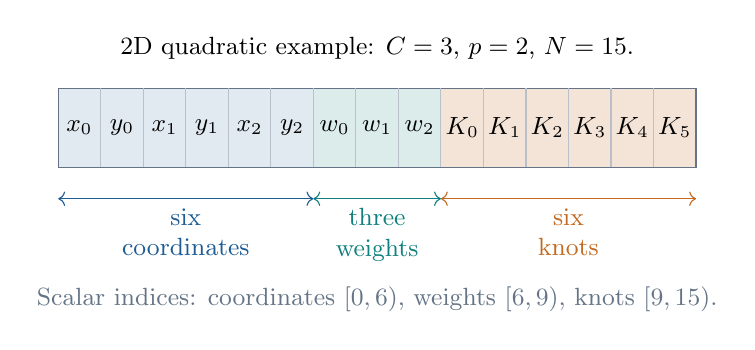
\begin{tikzpicture}[x=.54cm,y=1cm,font=\small]
\fill[manualblue!13] (0,0) rectangle (6,1);
\fill[manualteal!15] (6,0) rectangle (9,1);
\fill[manualorange!18] (9,0) rectangle (15,1);
\draw[manualmuted] (0,0) rectangle (15,1);
\foreach \x in {1,...,14} \draw[manualmuted!45] (\x,0)--(\x,1);
\foreach \x/\lab in {0/{x_0},1/{y_0},2/{x_1},3/{y_1},4/{x_2},5/{y_2},6/{w_0},7/{w_1},8/{w_2},9/{K_0},10/{K_1},11/{K_2},12/{K_3},13/{K_4},14/{K_5}}
 \node at (\x+.5,.5) {$\lab$};
\draw[<->,manualblue] (0,-.4)--(6,-.4)
 node[midway,below,align=center] {six\\coordinates};
\draw[<->,manualteal] (6,-.4)--(9,-.4)
 node[midway,below,align=center] {three\\weights};
\draw[<->,manualorange] (9,-.4)--(15,-.4)
 node[midway,below,align=center] {six\\knots};
\node[above,align=center] at (7.5,1.25)
 {2D quadratic example: $C=3$, $p=2$, $N=15$.};
\node[below,align=center,text=manualmuted] at (7.5,-1.4)
 {Scalar indices: coordinates $[0,6)$, weights $[6,9)$, knots $[9,15)$.};
\end{tikzpicture}
\caption{Flattened numeric ordering for an ordinary spline's indexed
parameters and an array-backed spline's public \api{parameters} storage.
Typed metadata is stored separately.}
\label{fig:spline-layout}
\end{figure}

\api{set_parameter(index,value)} returns \api{true} only if the full edited
candidate is accepted. It returns \api{false} for an invalid index or a rejected
definition, retaining the original state. Allocation failures can still
throw. This return-value convention differs from the named component setters,
whose invalid candidate or index is reported by an exception.

\api{set_parameters(const REAL*)} copies exactly
\api{number_of_parameters()} values in this ordering before validating.
The pointer is not retained. It must be nonnull and address a sufficiently
long readable buffer; the library cannot discover a raw pointer's extent.
For a complete numeric change, prepare a detached vector and call once:

\begin{lstlisting}[language=C++,caption={Indexed parameter names and one validated bulk copy.}]
std::vector<real> candidate(curve.number_of_parameters());
for (std::size_t i = 0; i < candidate.size(); ++i) {
    candidate[i] = curve.get_parameter(i);
    const std::string name = curve.parameter_name(i);
    static_cast<void>(name);
}
candidate[3] += 0.1;  // P[1].y in the 2D point-major layout.
auto scalar_edited = curve;
scalar_edited.set_parameters(candidate.data());
const bool accepted = scalar_edited.set_parameter(0, -0.2);
static_cast<void>(accepted);
\end{lstlisting}

There is no endpoint setter: an endpoint is derived from the definition.
Change the appropriate control-point definition, then read the refreshed
endpoint. Do not assume the first control point is always the active start:
that familiar identity depends on clamped endpoint knots.

\section{Array-backed curves for direct numeric work}
\label{sec:array-splines}

The array-backed classes are independent types, not subclasses of the
ordinary splines. They offer the same core geometry, checked setters, and
interpolation calls, plus a public \api{parameters} array and layout/range
queries. Their aliases \api{real_t} and \api{parameter_index_range} name the
scalar type and the allocation-free range of flattened scalar indices.

Construction can use endpoints with a control count and degree, component
vectors with a degree, a flattened \api{std::valarray<REAL>} with a degree,
or an explicit copy from the corresponding ordinary spline. The optional
closure and tolerance forms mirror these choices. The flattened constructor
derives $C$ from the scalar count $N$:
\begin{equation}
 \begin{array}{ll}
 \text{2D:}&N=4C+p+1,\\
 \text{3D:}&N=5C+p+1.
 \end{array}
\end{equation}
The inferred count must be integral and exceed the degree. A 2D sequence
cannot be interpreted as a 3D sequence simply by choosing another type.

\begin{lstlisting}[language=C++,caption={A flattened quadratic and same-world conversions.}]
const std::valarray<real> flat_quarter{
    1, 0,  1, 1,  0, 1,       // Three XY control points.
    1, std::sqrt(0.5), 1,       // Three weights.
    0, 0, 0, 1, 1, 1};        // Six knots.
np::nurbs_arr_spline2<real> array_quarter(flat_quarter, 2);

np::nurbs_arr_spline2<real> array_curve(curve);
np::nurbs_spline2<real> vector_curve(array_curve);
auto vector_copy = array_curve.to_nurbs_spline();
const point array_point = array_curve.evaluate(2.5);
\end{lstlisting}

These conversions copy the complete definition and preserve control points,
weights, knots, degree, tolerance, closure, and native domain. They validate
the current source array and can fail if it was edited into an invalid state.
The same operations exist between \api{nurbs_arr_spline3} and
\api{nurbs_spline3}. For shared ownership, the matching
\api{make_nurbs_spline2}, \api{make_nurbs_spline3},
\api{make_nurbs_arr_spline2}, and \api{make_nurbs_arr_spline3} allocation helpers
are covered in Chapter~\ref{chap:creators}. Ordinary allocation helpers also
accept component valarrays; that convenience overload does not turn an
ordinary curve into the flattened array-backed type.

\subsection{Direct editing, validation, and range meanings}

Direct array edits intentionally bypass checked setters. They can temporarily
leave invalid weights, bad knot order, a broken closed seam, or a malformed
array size. \api{validate()} checks the current layout, values, native domain,
and required seam. Geometric operations perform their own current-state
validation before using the array; they reject malformed storage before
indexing through its inferred layout.

No endpoint or other geometry cache is retained. \api{get_start()},
\api{get_end()}, \api{s_min()}, and \api{s_max()} derive their answers from
the current validated storage. Point getters reconstruct point values from
their coordinates; they do not alias adjacent scalars as a point object.
\api{get_control_points()}, \api{get_weights()}, and \api{get_knots()} return
detached vectors, unlike the ordinary spline getters' constant references.
Layout and component-access getters check shape; call \api{validate()} when
the whole definition, including numerical values and closure, must be checked.
\api{number_of_parameters()} reports the public array size even if its current
shape is malformed.

\api{control_point_count()}, \api{weight_count()}, and \api{knot_count()}
report component counts. The three range getters return \emph{flattened
scalar indices}, despite the word \api{count} in their names:

\begin{center}
\small
\begin{tabularx}{\linewidth}{@{}lXX@{}}
\toprule
Range getter & 2D indices & 3D indices\\
\midrule
\api{get_control_point_count_range()} & $[0,2C)$ & $[0,3C)$\\
\api{get_weight_count_range()} & $[2C,3C)$ & $[3C,4C)$\\
\api{get_knot_count_range()} & $[3C,N)$ & $[4C,N)$\\
\bottomrule
\end{tabularx}
\end{center}

\begin{lstlisting}[language=C++,caption={Use scalar ranges without assuming their offsets.}]
auto optimized = array_curve;
for (const auto i : optimized.get_weight_count_range()) {
    optimized.parameters[i] *= 1.25;
}
optimized.validate();

auto proposed = optimized.parameters;  // Detached valarray copy.
proposed[3] += 0.2;                    // Modify P[1].y.
optimized.set_parameters(proposed);    // Check before committing.
\end{lstlisting}

A range captures bounds when requested. Obtain a new range after replacing
or resizing \api{parameters}; do not reuse stale bounds. To preserve atomic
updates, prefer the array-specific
\api{set_parameters(std::valarray<REAL>)} or the common checked setter
families. The raw-pointer overload copies the current array's scalar count
and supports a source pointer into that current storage by detaching first.
\api{set_parameter} additionally returns \api{false} for a malformed current
shape, while allocation failure can still throw.

\subsection{Choosing the storage contract}

Use an ordinary spline when callers should see a continuously valid object
with private storage, stable metadata access, and cached endpoint queries.
Use an array-backed spline when numeric fitting code needs an openly
replaceable scalar array and can take responsibility for validating its
edits. Both evaluate in their own Cartesian world and use analytic
derivatives. Neither conversion nor direct array arithmetic is a coordinate
transform.

The persistence, projection, drawing, distance, and intersection interfaces
are documented with their accepted types in later chapters and the API
reference. When an operation accepts an ordinary spline specifically, call
\api{to_nurbs_spline()} explicitly; do not assume inheritance or an implicit
conversion. The ordinary 3D spline supplies \api{tag_write} and its static
\api{tag_read}; array-backed splines can use an explicit ordinary conversion
for that 3D tagged representation.

\chapter{Intersections, distances, and numerical tools}
\label{chap:algorithms}

An intersection query asks where a one-dimensional entity meets a circle,
sphere, or plane. A distance query asks for a closest point as well as its
parameter. These two questions share numerical machinery, but their results
have different meanings: an empty intersection set does not say how far apart
the entities are, and a distance rounded to zero does not create an intersection
record.

The examples in this chapter use \api{namespace np = nurbspath;} and
\api{using REAL = double;}, with the umbrella header included. All native 2D
queries stay entirely in the 2D world. An explicit \api{project(plane, entity)}
constructs a 3D entity when an application deliberately wants to cross that
boundary; it is not an implementation step of a 2D intersection or distance.

\section{Choose a query and its controls}

\begin{table}[htbp]
\centering
\small
\begin{tabularx}{\linewidth}{@{}l Y l@{}}
\toprule
World & Named intersection function & Result type \\
\midrule
2D & \api{intersect_ray_circle(ray, circle, settings)} & \api{intersection_result2<REAL>} \\
2D & \api{intersect_spline_circle(spline, circle, settings)} & \api{intersection_result2<REAL>} \\
3D & \api{intersect_ray_sphere(ray, sphere, settings)} & \api{intersection_result3<REAL>} \\
3D & \api{intersect_ray_plane(ray, plane, settings)} & \api{intersection_result3<REAL>} \\
3D & \api{intersect_spline_sphere(spline, sphere, settings)} & \api{intersection_result3<REAL>} \\
3D & \api{intersect_spline_plane(spline, plane, settings)} & \api{intersection_result3<REAL>} \\
\bottomrule
\end{tabularx}
\caption{The six supported intersection pairs. Each also has an
\api{intersect(first, second, settings)} convenience overload with the same
argument order and behavior.}
\label{tab:intersection-pairs}
\end{table}

The first argument is always the ray or ordinary NURBS spline. These overloads
do not provide arbitrary entity-pair intersections: there is no ray--ray,
spline--spline, sphere--sphere, circle--circle, or reversed-argument overload.
For an array-backed spline, first construct its corresponding ordinary spline
explicitly; that conversion validates the current public array storage.

\needspace{12\baselineskip}
\subsection{Two tolerances, two different units}

\api{numerical_settings<REAL>} carries all controls for numerical
intersections and point-to-spline distances. The defaults are:
\par\noindent\begin{minipage}{\linewidth}
\begin{lstlisting}[language=C++]
np::numerical_settings<REAL> settings;
// residual_tolerance = 1.0000e-08
// parameter_tolerance = 1.0000e-10
// max_iterations = 100
// sample_count = 256

settings.residual_tolerance = 1.0000e-07;
settings.parameter_tolerance = 1.0000e-09;
settings.sample_count = 512;
settings.validate();
\end{lstlisting}
\end{minipage}\par
\api{residual_tolerance} is measured in the units of the supplied function's
result. For the library's surface intersections, the residual is a signed
world distance; for \api{find_roots} it has whatever units the callable returns.
\api{parameter_tolerance} measures a parameter interval. For spline queries it
uses the original knot-domain units, not a normalized fraction of the domain.
Changing a spline's native domain therefore changes the interpretation of a
fixed parameter tolerance.

\api{sample_count} is the number of initial uniform intervals, so a sampled
search evaluates \api{sample_count + 1} initial positions. The iteration limit
applies to each refinement, rather than being a budget shared by all contacts
or local minima. Increase sampling density when a curve or residual oscillates
rapidly, has tightly spaced contacts, or has narrow distance minima.

\api{validate()} throws \api{std::invalid_argument} unless both tolerances are
finite and strictly positive, \api{max_iterations} is positive, and
\api{sample_count} is at least two. The numerical query functions call this
validation themselves. A larger iteration budget sharpens a basin that was
found; it cannot recover a basin that the initial sampling missed.

\begin{manualnote}[What a sampled answer guarantees]
Sampling and local refinement provide useful coverage controlled by
\api{sample_count}. They do not establish an unconditional continuous global
guarantee for every NURBS curve or user-supplied function. Check stability under
increased sampling when the application requires confidence that all contacts
or the smallest distance have been found.
\end{manualnote}

\section{Read an intersection result}

\api{intersection_kind} has three values. \api{none} means that the query found
no contact in its searched domain; \api{discrete} means that isolated contacts
are listed; \api{coincident} denotes a continuous overlap that a finite list of
points cannot represent. A coincident result deliberately has an empty
\api{points} vector. Thus \api{points.empty()} alone cannot distinguish no
contact from continuous overlap. Use \api{has_intersection()} to accept either
kind of contact, and \api{is_coincident()} to branch on continuous overlap.

\begin{table}[htbp]
\centering
\small
\begin{tabularx}{\linewidth}{@{}l Y Y@{}}
\toprule
Field & \api{intersection2<REAL>} & \api{intersection3<REAL>} \\
\midrule
\api{point} & Contact position in 2D & Contact position in 3D \\
\api{s} & Native ray or spline parameter & Native ray or spline parameter \\
\api{u} & Circle angle in $[0,2\pi)$ & Sphere longitude or plane $u$ coordinate \\
\api{v} & Not present & Sphere latitude or plane $v$ coordinate \\
\api{residual} & Absolute circle-distance residual & Absolute sphere- or plane-distance residual \\
\bottomrule
\end{tabularx}
\caption{A contact preserves both the world position and the participating
entities' parameters. Sphere latitude lies in $[-\pi/2,\pi/2]$; plane parameters
are lengths along its orthonormal local frame.}
\end{table}

The vector \api{points} is sorted by increasing \api{s}. Numerically close
root parameters are merged; the root solver's merge threshold is the greater
of four parameter tolerances and a roundoff allowance proportional to the
search interval. This is a parameter-based rule, not a promise to merge every
pair of spatially close points. A self-intersecting spline can visit the same
world position at two distinct native parameters, and those visits can remain
two distinct contacts.

\begin{figure}[htbp]
\centering
\begin{minipage}{0.48\linewidth}
\centering
\begin{tikzpicture}
\begin{axis}[width=\linewidth,height=5.0cm,axis equal image,
 xmin=-3.3,xmax=1.5,ymin=-1.45,ymax=1.55,
 axis lines=middle,xlabel={$x$},ylabel={$y$},
 ticks=none,clip=false]
\addplot[manualblue,thick,domain=0:360,samples=97]
 ({cos(x)},{sin(x)});
\addplot[manualred,thick,-{Stealth}] coordinates {(-3,0) (1.35,0)};
\addplot[only marks,mark=*,mark size=2.4pt,manualink]
 table[x index=1,y index=2] {pictures/intersection_crossing.dat};
\node[below left] at (axis cs:-3,0) {$O$};
\node[below] at (axis cs:-1,0) {$s=1$};
\node[below] at (axis cs:1,0) {$s=2$};
\node[above] at (axis cs:-1.9,0) {$\mathbf d=(2,0)$};
\end{axis}
\end{tikzpicture}
\end{minipage}\hfill
\begin{minipage}{0.48\linewidth}
\centering
\begin{tikzpicture}
\begin{axis}[width=\linewidth,height=5.0cm,axis equal image,
 xmin=-2.4,xmax=1.5,ymin=-1.45,ymax=1.55,
 axis lines=middle,xlabel={$x$},ylabel={$y$},
 ticks=none,clip=false]
\addplot[manualblue,thick,domain=0:360,samples=97]
 ({cos(x)},{sin(x)});
\addplot[manualred,thick,-{Stealth}] coordinates {(-2,1) (1.35,1)};
\addplot[only marks,mark=*,mark size=2.4pt,manualink]
 table[x index=1,y index=2] {pictures/intersection_tangent.dat};
\node[above left] at (axis cs:-2,1) {$O$};
\node[above right] at (axis cs:0,1) {$s=2$};
\node[below left] at (axis cs:-0.75,1) {$\mathbf d=(1,0)$};
\end{axis}
\end{tikzpicture}
\end{minipage}\par
\caption{Crossing and tangent ray--circle contacts. The black points are
computed by the library; TikZ constructs the unit circles and rays. The tangent
contact has no residual sign change.}
\label{fig:ray-circle-contacts}
\end{figure}

\section{Rays: forward domains and direction scales}

\subsection{A ray through a circle or sphere}

The ray equation is $R(s)=O+s\mathbf d$, with $s\geq0$. A direction is
not normalized by the entity. For the left-hand example in
Figure~\ref{fig:ray-circle-contacts}, each increase of one in $s$ moves two
world units. This gives the two unit-circle contacts at $s=1$ and $s=2$.
\par\noindent\begin{minipage}{\linewidth}
\begin{lstlisting}[language=C++]
const np::ray2<REAL> ray{{-3, 0}, {2, 0}};
const np::circle2<REAL> circle{{0, 0}, 1};
const auto hits = np::intersect_ray_circle(ray, circle);
// Equivalent: np::intersect(ray, circle)

std::cout << std::scientific << std::setprecision(4);
if (hits.kind == np::intersection_kind::discrete) {
    for (const auto& hit : hits.points) {
        std::cout << hit.s << ' ' << hit.point.x << ' '
                  << hit.point.y << '\n';
    }
}
\end{lstlisting}
\end{minipage}\par
The rounded output is:
\par\noindent\begin{minipage}{\linewidth}
\begin{lstlisting}
1.0000e+00 -1.0000e+00 0.0000e+00
2.0000e+00  1.0000e+00 0.0000e+00
\end{lstlisting}
\end{minipage}\par
The 3D counterpart changes the target from a circle to a sphere:
\par\noindent\begin{minipage}{\linewidth}
\begin{lstlisting}[language=C++]
const np::ray3<REAL> ray3{{-3, 0, 0}, {2, 0, 0}};
const np::sphere3<REAL> sphere{{0, 0, 0}, 1};
const auto sphere_hits = np::intersect_ray_sphere(ray3, sphere);
// Equivalent: np::intersect(ray3, sphere)
\end{lstlisting}
\end{minipage}\par
Both radial queries refine the signed distance
\[
 f(t)=\|O+t\widehat{\mathbf d}-C\|-r
\]
using world-distance travel $t$, then return the native parameter
$s=t/\|\mathbf d\|$. The finite forward search extends to
$\|O-C\|+r+\varepsilon_r$. Scaling the direction by a positive factor therefore
preserves world contacts while dividing their native $s$ values by that factor.
A negative factor reverses the forward half-line and can change the set of
contacts. A ray starting inside a circle or sphere normally has one forward
exit; a ray pointing away from the target may have none. Contact at the ray
origin is included.

\subsection{A ray and an infinite plane}

\api{intersect_ray_plane} uses the plane's unit normal and the signed
world-distance residual $f(s)=\widehat{\mathbf n}\mathbin{\cdot}(R(s)-P_0)$.
The native rate of change is $\mathbf d\mathbin{\cdot}\widehat{\mathbf n}$.
If that rate is exactly zero, an origin within residual tolerance gives
\api{coincident}; otherwise the result is \api{none}. This parallel test uses
a zero normal component rather than comparing the direction's magnitude to a
tolerance.

For a nonzero rate, an origin already within tolerance is an isolated contact
at $s=0$. Otherwise a negative estimated contact parameter means that the
plane is behind the ray. A forward contact is bracketed and refined through
the shared numerical root search. Refinement tightens the parameter tolerance
where needed for a large normal-direction rate.
\par\noindent\begin{minipage}{\linewidth}
\begin{lstlisting}[language=C++]
const np::plane3<REAL> plane{{0, 0, 0}, {0, 0, 1}};
const np::ray3<REAL> toward{{0.5, 0.25, 2}, {0, 0, -2}};
const auto plane_hit = np::intersect_ray_plane(toward, plane);
// Equivalent: np::intersect(toward, plane)
// One contact: s = 1, world point (0.5, 0.25, 0).

const np::ray3<REAL> parallel{{0, 0, 2}, {1, 0, 0}};
const np::ray3<REAL> contained{{0, 0, 0}, {1, 0, 0}};
const auto no_hit = np::intersect(parallel, plane);
const auto overlap = np::intersect(contained, plane);
// no_hit.kind == intersection_kind::none
// overlap.is_coincident() && overlap.points.empty()
\end{lstlisting}
\end{minipage}\par

\begin{figure}[htbp]
\centering
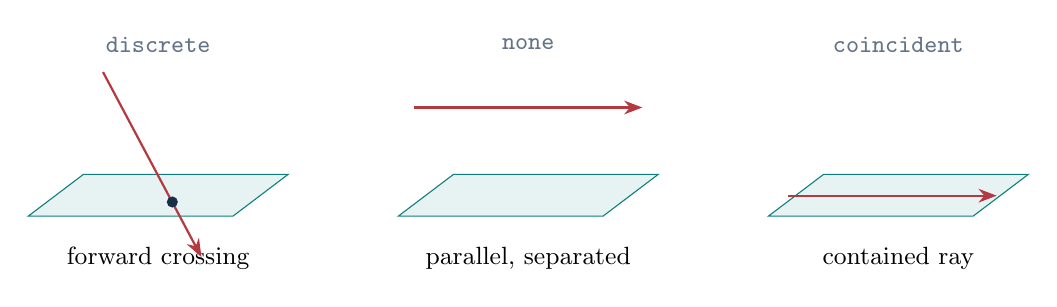
\begin{tikzpicture}[x=1cm,y=1cm,font=\small]
\foreach \x/\title in {0/{forward crossing},4.7/{parallel, separated},9.4/{contained ray}} {
  \begin{scope}[shift={(\x,0)}]
    \fill[manualteal!10] (-1.65,-0.18) -- (0.95,-0.18) -- (1.65,0.35) -- (-0.95,0.35) -- cycle;
    \draw[manualteal] (-1.65,-0.18) -- (0.95,-0.18) -- (1.65,0.35) -- (-0.95,0.35) -- cycle;
    \node at (0,-0.72) {\title};
  \end{scope}
}
\draw[manualred,thick,-{Stealth}] (-0.7,1.65) -- (0.55,-0.7);
\fill[manualink] (0.18,0) circle (2pt);
\draw[manualred,thick,-{Stealth}] (3.25,1.2) -- (6.15,1.2);
\draw[manualred,thick,-{Stealth}] (8.0,0.08) -- (10.65,0.08);
\node[manualmuted] at (0,2) {\api{discrete}};
\node[manualmuted] at (4.7,2) {\api{none}};
\node[manualmuted] at (9.4,2) {\api{coincident}};
\end{tikzpicture}
\caption{The three ray--plane classifications. The drawn patch represents an
infinite plane; its finite outline is only a diagram aid.}
\label{fig:ray-plane-cases}
\end{figure}

\section{Splines: crossings, tangencies, and continuous contact}

The three spline queries evaluate the full active interval
$[s_{\min},s_{\max}]$. Their residuals follow the target surface:
\begin{itemize}
\item \api{intersect_spline_circle} uses a 2D radial distance.
\item \api{intersect_spline_sphere} uses a 3D radial distance.
\item \api{intersect_spline_plane} uses the plane's signed distance.
\end{itemize}
Their \api{intersect} aliases preserve exactly these domains and meanings.

A compact degree-one example makes the native domain visible:
\par\noindent\begin{minipage}{\linewidth}
\begin{lstlisting}[language=C++]
const np::nurbs_spline2<REAL> segment2{
    std::vector<np::point2<REAL>>{{-2, 0}, {2, 0}},
    std::vector<REAL>{1, 1},
    std::vector<REAL>{10, 10, 14, 14}, 1};
const np::circle2<REAL> unit_circle{{0, 0}, 1};
const auto circle_hits = np::intersect_spline_circle(
    segment2, unit_circle, settings);
// Native s values are approximately 11 and 13, not 0.25 and 0.75.

const np::nurbs_spline3<REAL> segment3{
    std::vector<np::point3<REAL>>{{-2, 0, 0}, {2, 0, 0}},
    std::vector<REAL>{1, 1},
    std::vector<REAL>{10, 10, 14, 14}, 1};
const np::sphere3<REAL> unit_sphere{{0, 0, 0}, 1};
const np::plane3<REAL> yz_plane{{0, 0, 0}, {1, 0, 0}};
const auto sphere_contacts = np::intersect_spline_sphere(
    segment3, unit_sphere, settings);
const auto plane_contact = np::intersect_spline_plane(
    segment3, yz_plane, settings);
// Sphere: s approximately 11 and 13. Plane: s approximately 12.
\end{lstlisting}
\end{minipage}\par
Endpoints are included. A tangent contact may have residual zero with the same
sign on both sides, so the search does more than look for sign changes. It also
refines sampled local minima of the absolute residual. Increasing
\api{sample_count} remains necessary when tangencies lie in narrow or crowded
features.

Before returning isolated roots, each spline query checks whether the surface
residual stays within tolerance at a uniform set of
$\max(\api{sample_count},16)+1$ points. If so, it returns \api{coincident}.
This classification is numerical and sampled: it is not an algebraic proof
that the entire rational curve lies on the surface. A spline contained in a
plane or tracing a circle on a sphere is a natural use case.

For a spline explicitly marked closed, a root at the last active parameter is
removed when roots are already present within parameter tolerance of both
domain ends. The first-end contact remains as the seam representative. Closure
does not mean that arbitrary equal world positions elsewhere on the curve are
merged, and it does not itself imply periodic derivatives.

\begin{figure}[htbp]
\centering
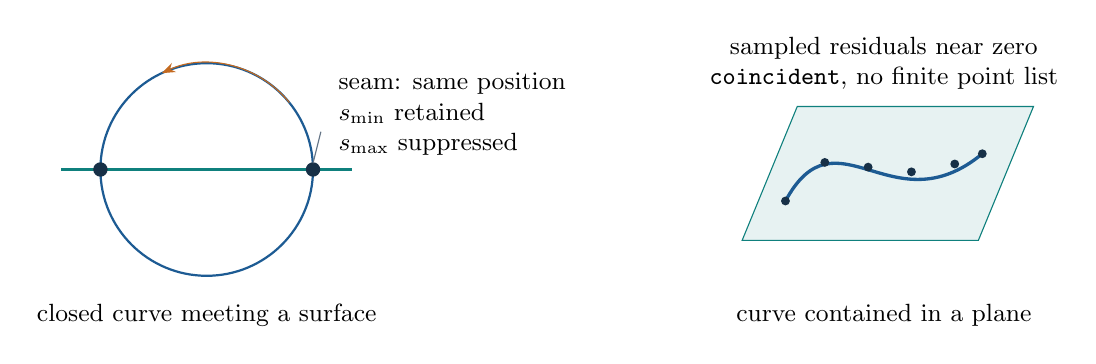
\begin{tikzpicture}[x=1cm,y=1cm,font=\small]
\begin{scope}
\draw[manualblue,thick] (0,0) circle (1.35);
\draw[manualteal,thick] (-1.85,0) -- (1.85,0);
\fill[manualink] (1.35,0) circle (2.6pt);
\fill[manualink] (-1.35,0) circle (2.6pt);
\draw[manualorange,-{Stealth}] (1.05,0.85) arc[start angle=39,end angle=115,radius=1.35];
\node[anchor=west,align=left] at (1.55,0.7) {seam: same position\\$s_{\min}$ retained\\$s_{\max}$ suppressed};
\draw[manualmuted] (1.45,0.48) -- (1.35,0.08);
\node at (0,-1.85) {closed curve meeting a surface};
\end{scope}
\begin{scope}[shift={(8.6,0)}]
\fill[manualteal!10] (-1.8,-0.9) -- (1.2,-0.9) -- (1.9,0.8) -- (-1.1,0.8) -- cycle;
\draw[manualteal] (-1.8,-0.9) -- (1.2,-0.9) -- (1.9,0.8) -- (-1.1,0.8) -- cycle;
\draw[manualblue,very thick] (-1.25,-0.4) .. controls (-0.6,0.8) and (0.1,-0.75) .. (1.25,0.2);
\foreach \x/\y in {-1.25/-0.4,-0.75/0.09,-0.2/0.03,0.35/-0.03,0.9/0.07,1.25/0.2}
 \fill[manualink] (\x,\y) circle (1.6pt);
\node[align=center] at (0,1.35) {sampled residuals near zero\\\api{coincident}, no finite point list};
\node at (0,-1.85) {curve contained in a plane};
\end{scope}
\end{tikzpicture}
\caption{Closed-seam deduplication and sampled continuous-contact detection.
The left-hand surface is shown by its trace through the curve's drawing
plane. The right-hand dots illustrate residual checks rather than isolated
intersection records.}
\label{fig:seam-coincidence}
\end{figure}

\section{Distances return geometry, not just a number}

The detailed queries in \api{distance.hpp} keep the closest world point and
its target parameter. The corresponding \api{distance} overload calls the
detailed function and returns only its \api{distance} field. Argument order is
always query point first, target entity second.

\begin{table}[htbp]
\centering
\small
\begin{tabularx}{\linewidth}{@{}l Y Y@{}}
\toprule
World & Detailed query & Result and target parameters \\
\midrule
2D & \api{distance_to_circle(point, circle, tolerance)} & \api{point_circle_distance2<REAL>}: \api{u} \\
2D & \api{distance_to_spline(point, spline, settings)} & \api{point_spline_distance2<REAL>}: \api{s} \\
3D & \api{distance_to_plane(point, plane, tolerance)} & \api{point_surface_distance3<REAL>}: \api{u}, \api{v} \\
3D & \api{distance_to_sphere(point, sphere, tolerance)} & \api{point_surface_distance3<REAL>}: \api{u}, \api{v} \\
3D & \api{distance_to_spline(point, spline, settings)} & \api{point_spline_distance3<REAL>}: \api{s} \\
\bottomrule
\end{tabularx}
\caption{Every result also has \api{distance} and \api{closest_point} fields.
The scalar alternative for each row is
\api{distance(point, target, tolerance_or_settings)}.}
\label{tab:distance-pairs}
\end{table}

All reported distances are nonnegative. When the measured separation is at
most the contact tolerance, the returned scalar is snapped to zero; the closest
point and its parameters remain those calculated on the target. A zero result
therefore permits a small geometric gap. For a spline, the contact tolerance
is \api{settings.residual_tolerance}; for a circle, sphere, or plane, the
separate tolerance argument defaults to \api{1.0000e-08}.

\subsection{Circle and sphere: radial closest points}

For a center $C$, radius $r$, and query $Q\ne C$,
\[
 P=C+r\frac{Q-C}{\|Q-C\|},\qquad
 d_{\mathrm{measured}}=\big|\|Q-C\|-r\big|.
\]
The expression applies in 2D to a circle and in 3D to a sphere. It finds the
closest point on the boundary, including when $Q$ is inside. At the center,
every boundary point is equally near; the library deterministically chooses
the positive world-$x$ point. Its circle angle is $u=0$, and its spherical
parameters are $(u,v)=(0,0)$.
\par\noindent\begin{minipage}{\linewidth}
\begin{lstlisting}[language=C++]
const np::circle2<REAL> circle{{0, 0}, 1};
const auto radial2 = np::distance_to_circle(
    np::point2<REAL>{3, 4}, circle);
// Rounded closest_point = (6.0000e-01, 8.0000e-01).
// Rounded distance = 4.0000e+00.
const REAL scalar2 = np::distance(np::point2<REAL>{3, 4}, circle);

const np::sphere3<REAL> sphere{{0, 0, 0}, 1};
const auto radial3 = np::distance_to_sphere(
    np::point3<REAL>{0, 0, 3}, sphere);
// closest_point = (0, 0, 1), distance = 2, v = pi/2.
const REAL scalar3 = np::distance(np::point3<REAL>{0, 0, 3}, sphere);
\end{lstlisting}
\end{minipage}\par
The circle-distance tolerance must be finite and strictly positive. The
plane- and sphere-distance overloads reject nonpositive tolerances; applications
should also supply finite values, consistently with the settings-based queries.

\subsection{Plane: orthogonal closest points}

Let $\widehat{\mathbf n}$ be the unit normal and $P_0$ its parameter origin.
Then
\[
 h=\widehat{\mathbf n}\mathbin{\cdot}(Q-P_0),\qquad
 P=Q-h\widehat{\mathbf n},\qquad d_{\mathrm{measured}}=|h|.
\]
The detailed query returns plane parameters of $P$, so
\api{plane.point_at(result.u, result.v)} reconstructs the closest position.
\api{plane.signed_distance_to(point)} remains available when the sign, rather
than the nonnegative distance query, is required.
\par\noindent\begin{minipage}{\linewidth}
\begin{lstlisting}[language=C++]
const np::plane3<REAL> plane{
    np::point3<REAL>{0, 0, 0}, np::vector3<REAL>{0, 0, 1},
    np::vector3<REAL>{1, 0, 0}};
const np::point3<REAL> query{2, 3, 4};
const auto nearest = np::distance_to_plane(query, plane);
// closest_point = (2, 3, 0), distance = 4, (u,v) = (2,3).
const REAL separation = np::distance(query, plane);
\end{lstlisting}
\end{minipage}\par

\begin{figure}[htbp]
\centering
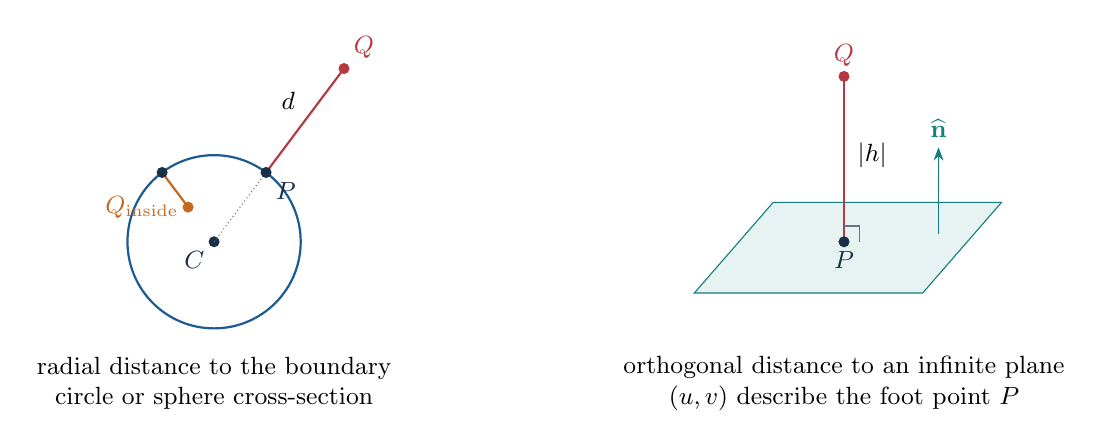
\begin{tikzpicture}[x=1cm,y=1cm,font=\small]
\begin{scope}
\draw[manualblue,thick] (0,0) circle (1.1);
\fill[manualink] (0,0) circle (2pt) node[below left] {$C$};
\draw[manualmuted,densely dotted] (0,0) -- (0.66,0.88);
\draw[manualred,thick] (0.66,0.88) -- (1.65,2.2);
\fill[manualink] (0.66,0.88) circle (2pt) node[below right] {$P$};
\fill[manualred] (1.65,2.2) circle (2pt) node[above right] {$Q$};
\node[above left] at (1.15,1.55) {$d$};
\fill[manualorange] (-0.33,0.44) circle (2pt) node[left] {$Q_{\rm inside}$};
\draw[manualorange,thick] (-0.33,0.44) -- (-0.66,0.88);
\fill[manualink] (-0.66,0.88) circle (2pt);
\node[align=center] at (0,-1.8) {radial distance to the boundary\\circle or sphere cross-section};
\end{scope}
\begin{scope}[shift={(8,0)}]
\fill[manualteal!10] (-1.9,-0.65) -- (1,-0.65) -- (2,0.5) -- (-0.9,0.5) -- cycle;
\draw[manualteal] (-1.9,-0.65) -- (1,-0.65) -- (2,0.5) -- (-0.9,0.5) -- cycle;
\draw[manualred,thick] (0,0) -- (0,2.1);
\draw[manualmuted] (0.2,0) -- (0.2,0.2) -- (0,0.2);
\fill[manualink] (0,0) circle (2pt) node[below] {$P$};
\fill[manualred] (0,2.1) circle (2pt) node[above] {$Q$};
\draw[manualteal,-{Stealth}] (1.2,0.1) -- (1.2,1.2) node[above] {$\widehat{\mathbf n}$};
\node[right] at (0.05,1.1) {$|h|$};
\node[align=center] at (0,-1.8) {orthogonal distance to an infinite plane\\$(u,v)$ describe the foot point $P$};
\end{scope}
\end{tikzpicture}
\caption{Analytic closest points for radial surfaces and planes. These
distances need no sampling. Interior radial queries still measure to the
surface, rather than returning zero throughout the filled region.}
\label{fig:analytic-distances}
\end{figure}

\section{Closest points on NURBS splines}

\api{distance_to_spline} minimizes the squared Euclidean separation
$D(s)=\|Q-C(s)\|^2$ over the active knot domain. Both 2D and 3D forms evaluate
the initial samples, retain the best sample, then refine each sampled local
basin using golden-section minimization. The first and last sample are also
eligible basins, with refinement over the adjacent boundary interval. This
matters when the true nearest point lies just inside an endpoint.

The same rational curve used in Chapter~\ref{chap:splines} provides a more
interesting distance example than a straight line:
\par\noindent\begin{minipage}{\linewidth}
\begin{lstlisting}[language=C++]
const np::nurbs_spline2<REAL> curve{
    std::vector<np::point2<REAL>>{
        {0, 0}, {1, 2}, {2, -1}, {3, 2}, {4, 0}},
    std::vector<REAL>{1, 1, 0.7, 1.5, 1},
    std::vector<REAL>{0, 0, 0, 0, 2, 5, 5, 5, 5}, 3};
const np::point2<REAL> query{2, 2.5};
const auto closest = np::distance_to_spline(query, curve, settings);
const REAL only_distance = np::distance(query, curve, settings);

// closest.s stays in the original [0,5] knot domain.
// curve.evaluate(closest.s) reproduces closest.closest_point.
\end{lstlisting}
\end{minipage}\par
Figure~\ref{fig:spline-closest} uses points evaluated by the library itself.
The target parameter remains the native $s$, even if its units were inherited
from interpolation stations. Neither the reported closest point nor the
distance query renormalizes the knot vector.

\begin{figure}[htbp]
\centering
\begin{tikzpicture}
\begin{axis}[width=0.88\linewidth,height=6.0cm,axis equal image,
 xmin=-0.2,xmax=4.2,ymin=-0.3,ymax=2.9,
 axis lines=left,xlabel={$x$},ylabel={$y$},
 xtick={0,1,2,3,4},ytick={0,1,2},grid=major,
 grid style={manualmuted!15},legend style={draw=none,font=\small},
 legend pos=south east]
\addplot[manualblue,very thick] table[x index=1,y index=2] {pictures/spline_curve.dat};
\addlegendentry{rational spline $C(s)$}
\addplot[manualred,thick,densely dashed,mark=*,mark size=2.3pt]
 table[x index=0,y index=1] {pictures/distance_reference.dat};
\addlegendentry{query-to-closest segment}
\node[above] at (axis cs:2,2.5) {$Q=(2,2.5)$};
\end{axis}
\end{tikzpicture}
\caption{A sampled and refined 2D closest point. The curve samples and the two
endpoints of the red distance segment come from the library reference-data
generator in \api{manual/pictures/}. The 3D distance overload follows the same
search strategy in its independent world.}
\label{fig:spline-closest}
\end{figure}

The 3D call has the same shape:
\par\noindent\begin{minipage}{\linewidth}
\begin{lstlisting}[language=C++]
const np::nurbs_spline3<REAL> segment{
    std::vector<np::point3<REAL>>{{0, 0, 0}, {1, 0, 0}},
    std::vector<REAL>{1, 1},
    std::vector<REAL>{0, 0, 1, 1}, 1};
const auto near_start = np::distance_to_spline(
    np::point3<REAL>{0.001, 0, 0}, segment, settings);
// closest point is just inside the segment, not its start endpoint.
// Reported distance is zero within residual_tolerance.
\end{lstlisting}
\end{minipage}\par
Endpoint retention prevents a refinement from discarding a true boundary
minimum, while boundary-interval refinement can improve a coarse endpoint
sample to an interior minimum. Multiple sampled minima are compared; no unique
closest-point guarantee is made for equal minima. In particular, a closed seam
or a symmetric curve can have more than one equally good parameter, while the
result type intentionally returns one.

\begin{figure}[htbp]
\centering
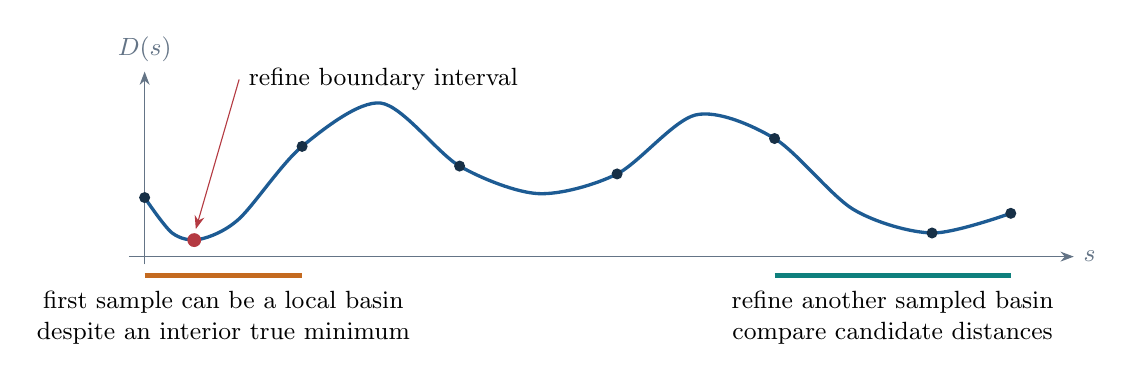
\begin{tikzpicture}[x=1cm,y=1cm,font=\small]
\draw[manualmuted,-{Stealth}] (-0.2,0) -- (11.8,0) node[right] {$s$};
\draw[manualmuted,-{Stealth}] (0,-0.1) -- (0,2.35) node[above] {$D(s)$};
\draw[manualblue,very thick] plot[smooth] coordinates {
 (0,0.75) (0.35,0.30) (0.7,0.22) (1.2,0.48) (2,1.4)
 (3,1.95) (4,1.15) (5,0.8) (6,1.05) (7,1.8)
 (8,1.5) (9,0.60) (10,0.30) (11,0.55)};
\foreach \x/\y in {0/0.75,2/1.4,4/1.15,6/1.05,8/1.5,10/0.30,11/0.55}
 \fill[manualink] (\x,\y) circle (2pt);
\draw[manualorange,line width=2pt] (0,-0.24) -- (2,-0.24);
\draw[manualteal,line width=2pt] (8,-0.24) -- (11,-0.24);
\fill[manualred] (0.63,0.21) circle (2.5pt);
\draw[manualred,-{Stealth}] (1.2,2.25) -- (0.65,0.35);
\node[anchor=west] at (1.2,2.25) {refine boundary interval};
\node[below,align=center] at (1,-0.32) {first sample can be a local basin\\despite an interior true minimum};
\node[below,align=center] at (9.5,-0.32) {refine another sampled basin\\compare candidate distances};
\end{tikzpicture}
\caption{Why closest-point searches refine more than the single best sample.
This schematic squared-distance graph illustrates a minimum near the beginning
of the domain and another basin near its end. It is not an additional library
test curve.}
\label{fig:distance-basins}
\end{figure}

\section{Reusable scalar algorithms}

The utilities in \api{utility.hpp} are public and independent of a particular
geometry class. Their callable parameters accept a scalar and return a scalar.
The application is responsible for choosing meaningful units, finite working
ranges, and functions compatible with the search assumptions.

\subsection{Find all sampled roots, including even-multiplicity contacts}

\api{find_roots<REAL>(function, lower, upper, settings)} requires a strictly
increasing interval. It samples that interval, refines sign changes with
bisection, and minimizes absolute residual near sampled sign-preserving local
minima. Contiguous within-tolerance sample bands are represented by a single
best candidate, avoiding a separate result for every sample on a flat contact.
The final roots are sorted and tolerance-deduplicated.
\par\noindent\begin{minipage}{\linewidth}
\begin{lstlisting}[language=C++]
const auto function = [](REAL x) {
    return (x + 0.8) * np::square(x - 0.3) * (x - 1.2);
};
const auto roots = np::find_roots<REAL>(
    function, -1.5, 1.6, settings);
for (REAL root : roots) {
    std::cout << std::scientific << std::setprecision(4)
              << root << '\n';
}
\end{lstlisting}
\end{minipage}\par
The three expected roots, shown as rounded reference values, are
$-8.0000\times10^{-1}$, $3.0000\times10^{-1}$, and
$1.2000\times10^{0}$. The middle root is double and does not change the sign
of the residual. \api{find_roots} rejects invalid settings or a nonpositive
interval length with \api{std::invalid_argument}; a nonfinite initial sample
value raises \api{std::domain_error}. A discontinuous callable or a nonfinite
value encountered during refinement falls outside a well-behaved root-search
problem; do not treat a sign change across a discontinuity as a root proof.

\begin{figure}[htbp]
\centering
\begin{tikzpicture}
\begin{axis}[width=0.88\linewidth,height=5.7cm,
 xmin=-1.5,xmax=1.6,ymin=-0.7,ymax=2.1,
 axis lines=middle,xlabel={$x$},ylabel={$f(x)$},
 xtick={-0.8,0.3,1.2},xticklabels={$-0.8$,$0.3$,$1.2$},
 ytick={0,1,2},grid=major,grid style={manualmuted!15},clip=true]
\addplot[manualblue,very thick] table[x index=0,y index=1] {pictures/algorithmroots.dat};
\addplot[only marks,mark=*,mark size=2.6pt,manualred]
 coordinates {(-0.8,0) (0.3,0) (1.2,0)};
\node[anchor=south,align=center] at (axis cs:0.3,0.2) {double root\\no sign change};
\draw[manualred,-{Stealth}] (axis cs:0.3,0.18) -- (axis cs:0.3,0.035);
\end{axis}
\end{tikzpicture}
\caption{The scalar residual
$f(x)=(x+0.8)(x-0.3)^2(x-1.2)$. Its sampled graph is generated by C++ using
the library's scalar helper; TikZ marks the known reference roots. Sign changes
alone would miss the contact at $x=0.3$.}
\label{fig:scalar-roots}
\end{figure}

\subsection{Refine one sign-changing bracket}

\api{bisect_root<REAL>(function, lower, upper, settings)} accepts endpoints in
either order. An endpoint whose absolute residual is already within tolerance
is returned immediately. Otherwise the endpoints must have opposite residual
signs, or \api{std::invalid_argument} is thrown. Each iteration keeps the
half-interval that still brackets the sign change. The function returns when
the residual is small enough, the interval is narrow enough, or the iteration
budget has been used.
\par\noindent\begin{minipage}{\linewidth}
\begin{lstlisting}[language=C++]
const REAL root_two = np::bisect_root<REAL>(
    [](REAL x) { return np::square(x) - 2; }, 1, 2, settings);
// Rounded: 1.4142e+00
\end{lstlisting}
\end{minipage}\par
The return type is a parameter alone: it does not carry an iteration count or
a convergence flag. In particular, reaching the parameter tolerance or the
iteration limit does not independently establish a small residual. Evaluate
the returned residual if the application requires that additional check.
Bisection is appropriate for a continuous sign-changing bracket; use the
sampled root finder to seek an unbracketed tangent contact.

\subsection{Minimize one bounded basin}

\api{golden_section_minimize<REAL>(function, lower, upper, settings)} also
accepts reversed endpoints. Two interior probes progressively contract a
closed interval, reusing one function value after each comparison. It returns
the center of the final interval, stopping at the parameter tolerance or
iteration limit. A unimodal objective over the chosen interval is the useful
working assumption. The function does not search every local minimum of an
arbitrary multi-basin objective, and it does not separately select endpoint
values; callers needing boundary minima should compare the endpoints too.
\par\noindent\begin{minipage}{\linewidth}
\begin{lstlisting}[language=C++]
const REAL minimum_x = np::golden_section_minimize<REAL>(
    [](REAL x) { return np::square(x - 0.75) + 2; },
    -1, 2, settings);
// Rounded minimizer: 7.5000e-01; objective value: 2.0000e+00.
\end{lstlisting}
\end{minipage}\par
Both refiners call \api{settings.validate()}. Golden-section search uses
\api{parameter_tolerance} and \api{max_iterations} to stop; changing
\api{residual_tolerance} does not supply a separate objective-value stopping
rule. It is nevertheless validated as part of the settings object.

\begin{figure}[htbp]
\centering
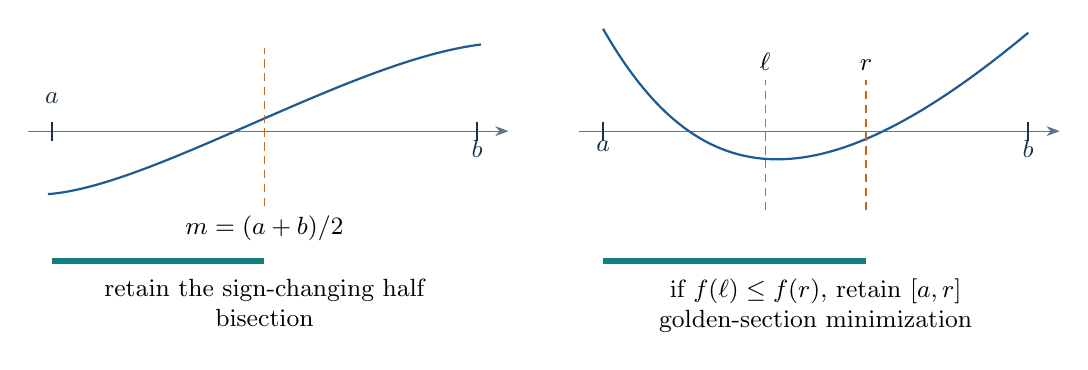
\begin{tikzpicture}[x=1cm,y=1cm,font=\small]
\begin{scope}
\draw[manualmuted,-{Stealth}] (-0.3,0) -- (5.8,0);
\draw[manualblue,thick] (-0.05,-0.8) .. controls (1.3,-0.7) and (3.8,0.9) .. (5.45,1.1);
\draw[manualink,thick] (0,-0.12) -- (0,0.12) node[above=3pt] {$a$};
\draw[manualink,thick] (5.4,-0.12) -- (5.4,0.12) node[below=3pt] {$b$};
\draw[manualorange,densely dashed] (2.7,-0.95) -- (2.7,1.05);
\node[below] at (2.7,-0.95) {$m=(a+b)/2$};
\draw[manualteal,line width=2pt] (0,-1.65) -- (2.7,-1.65);
\node[below,align=center] at (2.7,-1.75) {retain the sign-changing half\\bisection};
\end{scope}
\begin{scope}[shift={(7,0)}]
\draw[manualmuted,-{Stealth}] (-0.3,0) -- (5.8,0);
\draw[manualblue,thick] (0,1.3) .. controls (1.2,-0.8) and (2.7,-1.0) .. (5.4,1.25);
\draw[manualink,thick] (0,-0.12) -- (0,0.12) node[below=3pt] {$a$};
\draw[manualink,thick] (5.4,-0.12) -- (5.4,0.12) node[below=3pt] {$b$};
\draw[manualorange,densely dashed] (2.06,-1) -- (2.06,0.65);
\draw[manualorange,densely dashed] (3.34,-1) -- (3.34,0.65);
\node[above] at (2.06,0.65) {$\ell$};
\node[above] at (3.34,0.65) {$r$};
\draw[manualteal,line width=2pt] (0,-1.65) -- (3.34,-1.65);
\node[below,align=center] at (2.7,-1.75) {if $f(\ell)\leq f(r)$, retain $[a,r]$\\golden-section minimization};
\end{scope}
\end{tikzpicture}
\caption{A root refiner and a minimum refiner answer different questions.
The green segments show one possible retained interval. The diagrams are
schematic; neither refiner reports a continuous global-search certificate.}
\label{fig:scalar-refiners}
\end{figure}

\section{Linear systems and small helpers}

\subsection{Solve a square system}

\api{solve_linear_system(matrix, right_hand_side, pivot_tolerance)} solves
$A\mathbf x=\mathbf b$ by elimination with scaled partial pivoting. Each row's
largest absolute entry supplies a scale, so the pivot comparison is relative
to that row's magnitude. The matrix and right-hand-side arguments are passed
by value and copied for elimination; the caller's containers are preserved.

\par\noindent\begin{minipage}{\linewidth}
\begin{lstlisting}[language=C++]
const std::vector<std::vector<REAL>> matrix{{2, 1}, {1, 3}};
const std::vector<REAL> right_hand_side{5, 10};
const auto solution = np::solve_linear_system(matrix, right_hand_side);
// Rounded solution: {1.0000e+00, 3.0000e+00}.
\end{lstlisting}
\end{minipage}\par
The default pivot rejection threshold is
$64\,\api{std::numeric_limits<REAL>::epsilon()}$. The function requires a
nonempty square matrix and a matching right-hand side, otherwise it throws
\api{std::invalid_argument}. A zero row or a pivot too small relative to its
row scale raises \api{std::domain_error}, identifying a singular or rejected
ill-conditioned system. Use finite coefficients and a sensible finite
nonnegative pivot threshold; this is a small dense solver, not a rank-revealing
factorization or a condition-number estimator. Global interpolation uses this
reusable solver rather than duplicating it inside spline classes.

\subsection{Square, absolute comparison, and definition sizing}

\api{square(value)} returns \api{value * value}; it is \api{constexpr} and
\api{noexcept}, with ordinary floating-point range and rounding behavior.
It does not trap an overflow. \api{approximately_equal(first, second, tolerance)}
returns whether the absolute difference is at most the supplied tolerance.
It performs no relative scaling and does not validate the tolerance. Select a
nonnegative tolerance in the compared quantities' units. For example, a fixed
absolute tolerance suitable for millimeter coordinates need not suit the same
data expressed in kilometers.

\api{nurbs_knot_count(degree, control_point_count)} returns
$C+p+1$. It is shared by both worlds and both spline storage forms. The degree
must be positive and smaller than the control-point count; invalid values
raise \api{std::invalid_argument}. An unrepresentable result raises
\api{std::overflow_error}. This helper sizes the complete knot vector; it does
not generate knot values or decide whether a candidate vector is clamped.
\par\noindent\begin{minipage}{\linewidth}
\begin{lstlisting}[language=C++]
constexpr std::size_t knots_needed = np::nurbs_knot_count(3, 5);
static_assert(knots_needed == 9);
const REAL area_factor = np::square(REAL(2.5));
const bool close = np::approximately_equal(
    REAL(1), REAL(1) + REAL(5.0000e-09), REAL(1.0000e-08));
// area_factor rounds to 6.2500e+00; close is true.
\end{lstlisting}
\end{minipage}\par

For two points in the same world, \api{distance_squared(first, second)} and
\api{distance(first, second)} are also available from their point headers.
They return ordinary squared Euclidean distance and Euclidean distance,
respectively, without contact snapping or a search. Unlike the target-entity
distance overloads, they need neither a tolerance nor numerical settings.

\begin{manualnote}[A practical verification pattern]
Preserve the parameters and world positions from detailed results when they
matter to downstream work. Re-evaluate the entity at those parameters, inspect
the residual, and repeat sampled queries at higher sampling density when
coverage is uncertain. Round only presentation output; keep the underlying
floating-point values for subsequent calculations and persistence.
\end{manualnote}

\chapter{Rendering, persistence, and diagnostics}\label{chap:output}
\section{A flat native 2D canvas}
\api{svg_view2<REAL>} maps the independent 2D world directly onto a rectangular
SVG image. Supply its world centre, minimum visible world width and height,
and optional image dimensions. The mapping uses one uniform scale; a viewport
with a different aspect ratio is letterboxed rather than stretching circles
into ellipses. Positive world $y$ points up while SVG image $y$ points down.

\begin{lstlisting}
namespace np = nurbspath;
using REAL = double;
const np::svg_view2<REAL> view({0.0, 0.0}, 6.0, 4.0, 900, 600);
np::svg_graphics_options2<REAL> style;
style.line_width = 1.5;
style.spline_segment_count = 160;
np::svg_canvas2<REAL> canvas(view, style);
canvas.add(np::point2<REAL>{-1.0, 1.0});
canvas.add(np::ray2<REAL>({-2.0, -1.0}, {1.0, 0.25}));
canvas.add(np::circle2<REAL>({0.5, 0.0}, 1.0));
const std::string svg = canvas.svg();
// canvas.write(output) streams the same self-contained document.
\end{lstlisting}
The canvas accepts native 2D points, rays, circles, and ordinary splines.
\api{add(spline)} draws its sampled polyline, control polygon, controls, and
evaluated endpoint dots. All flat-canvas strokes are solid, including
construction geometry. Unit red/green $XY$ references remain visible at the
2D origin. Vectors cannot be drawn alone because they do not supply a position.

\begin{figure}[htbp]\centering
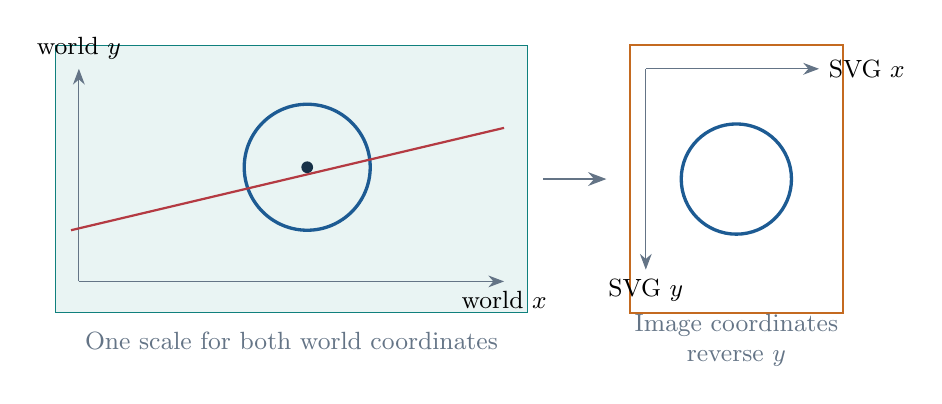
\begin{tikzpicture}[x=1cm,y=1cm]
 \draw[surface] (-3,-1.7) rectangle (3,1.7);
 \draw[axis] (-2.7,-1.3)--(2.7,-1.3) node[below] {world $x$};
 \draw[axis] (-2.7,-1.3)--(-2.7,1.4) node[above] {world $y$};
 \draw[curve] (.2,.15) circle (.8);
 \node[point] at (.2,.15) {};
 \draw[manualred,thick] (-2.8,-.65)--(2.7,.65);
 \node[manualmuted] at (0,-2.05) {One scale for both world coordinates};
 \draw[manualorange,thick] (4.3,-1.7) rectangle (7.0,1.7);
 \draw[axis] (4.5,1.4)--(6.7,1.4) node[right] {SVG $x$};
 \draw[axis] (4.5,1.4)--(4.5,-1.15) node[below] {SVG $y$};
 \draw[curve] (5.65,0) circle (.7);
 \node[manualmuted,align=center] at (5.65,-2.05) {Image coordinates\\reverse $y$};
 \draw[-{Stealth},manualmuted,thick] (3.2,0)--(4.0,0);
\end{tikzpicture}
\caption{A flat drawing needs no plane embedding. Uniform scale preserves
shape; the image coordinate direction is a display convention.}
\label{fig:flat-canvas}
\end{figure}

\section{World-space cameras in 3D}
\api{svg_view3<REAL>::orthographic} takes a world-space eyepoint and look-at
point, orthographic world width/height, and image dimensions.
\api{svg_view3<REAL>::perspective} instead takes the vertical field angle in
radians and a positive near distance. A camera must have a nonzero viewing
direction. Image dimensions and orthographic extents must be positive; a
perspective field angle must be strictly between zero and $\pi$. Camera
getters expose the selected settings without changing the camera.

\begin{lstlisting}
const np::point3<REAL> eye{5.0, -7.0, 4.5};
const np::point3<REAL> target{0.0, 0.0, 0.5};
const auto ortho = np::svg_view3<REAL>::orthographic(
    eye, target, 6.0, 4.0, 900, 600);
const auto perspective = np::svg_view3<REAL>::perspective(
    eye, target, std::numbers::pi_v<REAL> / 4.0,
    900, 600, 0.05);
np::svg_document3<REAL> scene(perspective);
scene.add(np::sphere3<REAL>({0.0, 0.0, 0.0}, 1.0));
scene.add(np::plane3<REAL>({0.0, 0.0, -1.0}, {0.0, 0.0, 1.0}));
scene.add(np::ray3<REAL>({-2.0, 0.0, 0.0}, {2.0, 0.0, 0.0}));
const std::string scene_svg = scene.svg();
\end{lstlisting}

\begin{figure}[htbp]\centering
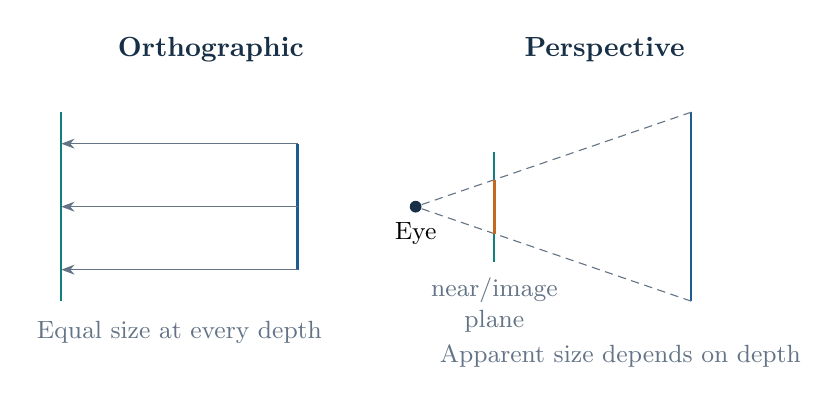
\begin{tikzpicture}[x=1cm,y=1cm]
 \node[manualink,font=\bfseries] at (1.9,2) {Orthographic};
 \draw[manualteal,thick] (0,-1.2)--(0,1.2);
 \draw[manualblue,thick] (3,-.8)--(3,.8);
 \foreach \y in {-.8,0,.8} \draw[-{Stealth},manualmuted] (3,\y)--(0,\y);
 \node[manualmuted] at (1.5,-1.6) {Equal size at every depth};
 \node[manualink,font=\bfseries] at (6.9,2) {Perspective};
 \node[point,label=below:Eye] (e) at (4.5,0) {};
 \draw[manualteal,thick] (5.5,-.7)--(5.5,.7);
 \draw[manualblue,thick] (8,-1.2)--(8,1.2);
 \draw[guide] (e)--(8,-1.2) (e)--(8,1.2);
 \draw[manualorange,very thick] (5.5,-.343)--(5.5,.343);
 \node[manualmuted,align=center] at (5.5,-1.25) {near/image\\plane};
 \node[manualmuted] at (7.1,-1.9) {Apparent size depends on depth};
\end{tikzpicture}
\caption{Camera projection is a display operation on the same 3D geometry.
The perspective diagram is a 2D cross-section of the viewing cone.}
\label{fig:camera-projection}
\end{figure}

Perspective world segments are clipped at the near plane before division by
depth. A segment crossing the plane retains its visible part; an entirely
hidden segment disappears. Orthographic output uses a uniform screen scale.
The sphere silhouette is sampled from geometry appropriate to the camera.

\begin{figure}[htbp]\centering
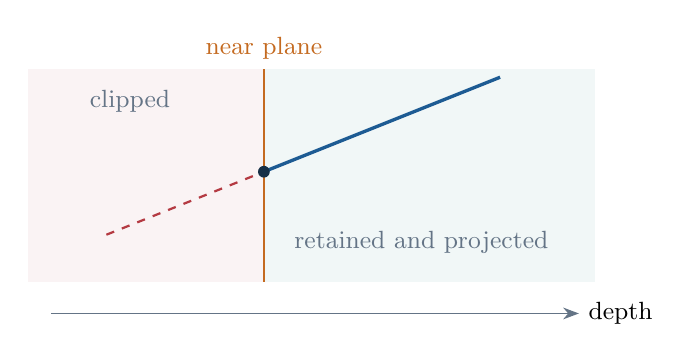
\begin{tikzpicture}
 \fill[manualred!6] (-3,-1.2) rectangle (0,1.5);
 \fill[manualteal!6] (0,-1.2) rectangle (4.2,1.5);
 \draw[manualorange,thick] (0,-1.2)--(0,1.5) node[above] {near plane};
 \draw[manualred,dashed,thick] (-2,-.6)--(0,.2);
 \draw[curve] (0,.2)--(3,1.4);
 \node[point] at (0,.2) {};
 \node[manualmuted] at (-1.7,1.1) {clipped};
 \node[manualmuted] at (2,-.7) {retained and projected};
 \draw[axis] (-2.7,-1.6)--(4,-1.6) node[right] {depth};
\end{tikzpicture}
\caption{Near-plane clipping prevents an invisible endpoint from producing
an unbounded perspective line. The clipped endpoint is an intermediate
rendering point, not a new library entity.}
\label{fig:near-clip}
\end{figure}

\section{Diagnostic glyphs and convenience rendering}
The default 3D scene is deliberately diagnostic rather than photorealistic.
The configurable \api{line_width} is in SVG viewBox units. The graphics options
also control spline/sphere segment counts, the plane square size, and other
documented construction lengths. \api{validate()} rejects invalid settings and
derived stroke sizes that cannot remain finite.

\begin{tabularx}{\linewidth}{@{}lY@{}}
\toprule
Entity & Default diagnostic conventions\\
\midrule
Point & Black location dot.\\
Ray & Pale-red dashed infinite supporting line, solid positive unit-direction
marker, and origin dot. Native direction magnitude does not change its glyph.\\
Sphere & Pale-blue silhouette, visible/hidden equator strokes, and centre dot.\\
Plane & Pale-green square (default side one quarter unit), unit normal,
half-unit positive $u$/$v$ markers, and parameter-origin dot.\\
Spline & Piecewise-linear curve, dashed control polygon, control dots, and
evaluated endpoint dots.\\
World axes & Persistent coloured $XYZ$ unit axes and labels at half line width.\\
\bottomrule
\end{tabularx}

A native 2D entity can be explicitly embedded for rendering with
\api{scene.add(plane, entity2)}. Its primary strokes are dash-dotted, with
dotted auxiliary/hidden/control strokes. The 2D circle bridge carries centre
and radius into a complete sphere. The separate flat canvas performs no such
embedding and always uses solid strokes.

\api{to_svg(view2, entity2, options2)} constructs a temporary flat canvas.
\api{to_svg(view3, entity3, options3)} constructs a 3D document.
\api{to_svg(view3, plane, entity2, options3)} performs explicit embedding. All
return self-contained XML strings; \api{svg()} and \api{write(output)} expose
the corresponding accumulated document. These functions do not render free
vectors or transform an arbitrary coordinate frame. A projected 2D circle
whose finite world radius overflows the screen radius has its outline omitted;
a finite centre still receives its dot.

\section{Coordinate streams, CSV/TSV, and binary records}
\api{point2}, \api{point3}, \api{vector2}, and \api{vector3} support
\api{operator<<} and \api{operator>>}. Their fields are whitespace-separated
coordinates in $x,y[,z]$ order. Reads commit only when a complete coordinate
record has been obtained. Vector/point semantics remain explicit even though
the scalar layout is similar.

\begin{lstlisting}
np::point3<REAL> position{1.0, 2.0, 3.0};
std::ostringstream csv;
position.csv_write(csv, np::text_format::csv, 4);
// Display: 1.0000e+00,2.0000e+00,3.0000e+00
std::istringstream csv_input(csv.str());
np::point3<REAL> restored;
restored.csv_read(csv_input, np::text_format::csv);
std::stringstream binary(std::ios::in | std::ios::out | std::ios::binary);
position.write(binary);
np::point3<REAL> binary_copy;
binary_copy.read(binary);
\end{lstlisting}
\api{csv_write(output, format, decimal_places)} uses scientific notation;
the default precision is six decimal places. Select \api{text_format::csv},
\api{tsv}, or \api{txt}. Delimited reads expect the chosen separators in the
coordinate record; this is not a general quoted-field CSV parser. These
helpers do not append a newline. Invalid format/negative output precision are
rejected. Stream errors use the normal stream state and exception mask.

Binary \api{write}/\api{read} store two or three native \api{REAL} values,
without a header or type discriminator. The layout is appropriate for matching
readers/writers, not portable interchange across byte orders, scalar types, or
floating-point representations. A failed complete read leaves the original
entity unchanged.

\section{Tagged records and independent presentation rows}
Tagged persistence supports four concrete 3D geometry types and three
presentation types. The scientific numbers in this displayed preview have
four decimal places; the canonical writers deliberately use full round-trip
\api{REAL} precision, independent of the destination stream formatting.

\begin{lstlisting}[style=plain]
42 point3 v1 1.0000e+00 2.0000e+00 3.0000e+00
42 vector3 v1 0.0000e+00 1.0000e+00 0.0000e+00
42 sphere3 v1 0.0000e+00 0.0000e+00 0.0000e+00 1.0000e+00
42 linecolor v1 2.0000e-01 4.0000e-01 8.0000e-01 7.5000e-01
42 linefont v1 1.5000e+00 4.0000e+00 2.0000e+00
42 text v1 1.2000e+01 "Path \"A\"\nnext pass"
\end{lstlisting}
\api{spline3} is the token for \api{nurbs_spline3}; its payload contains
degree, closure flag, tolerance, control and knot counts, interleaved control
$x,y,z,\text{weight}$ groups, then all knots. Array-backed splines convert to
an ordinary same-world spline before tagged output. There is no tagged 2D
geometry format or implicit 2D-to-3D persistence conversion.

\begin{tabularx}{\linewidth}{@{}lY@{}}
\toprule
Presentation value & Validation and meaning\\
\midrule
\api{line_color<REAL>} & \api{red}, \api{green}, \api{blue}, \api{alpha} are
finite in $[0,1]$. Alpha is opacity; default is opaque black.\\
\api{line_font<REAL>} & Finite positive width; \api{on}/\api{off} are both
zero for solid lines, or both finite positive for dashes. Default is
\api{{1,0,0}}.\\
\api{text_label<REAL>} & Finite positive size, default 12, and a string.
Width, dash lengths, and text size use consumer-selected display units.\\
\bottomrule
\end{tabularx}

\begin{lstlisting}
std::stringstream rows;
position.tag_write(42, rows);
np::line_color<REAL>{0.2, 0.4, 0.8, 0.75}.tag_write(42, rows);
np::line_font<REAL>{1.5, 4.0, 2.0}.tag_write(42, rows);
np::text_label<REAL>{12.0, "Path \"A\"\nnext pass"}.tag_write(42, rows);
while (auto record = np::tag_read_record<REAL>(rows)) {
    std::visit([tag = record->tag](const auto& owner) {
        // *owner has its concrete geometry or presentation type.
        (void)tag;
        (void)owner;
    }, record->value);
}
\end{lstlisting}

Tags are unsigned base-ten \api{std::size_t} application values, not unique
identifiers. Repeated tags, nonadjacent rows, and empty files are permitted.
The consumer chooses association, omitted-style defaults, and label placement.
Presentation rows do not alter SVG drawing state.

\api{T::tag_read(input)} returns
\api{std::optional<tagged_read_result<T>>}, with \api{tag} and a non-null
\api{std::shared_ptr<T>} named \api{entity}. A typed reader requires its
matching non-advisory type. \api{tag_read<REAL>} returns a
\api{tagged_entity3} whose \api{entity3_ptr} variant contains only point,
vector, sphere, and ordinary spline pointers. \api{tag_read_record<REAL>}
returns a \api{tagged_record} with the seven-type \api{value} variant.

Quoted labels escape backslash, double quote, newline, carriage return, and
tab. Each record remains one physical row. Other ASCII control bytes are
rejected; bytes at least 128 are preserved without UTF-8 validation. Writers
validate public fields before emitting invalid data.

\section{Advisory application and positioned messages}
\api{application_info} writes an untagged row with two nonempty, unquoted
tokens. ASCII whitespace/control bytes are not allowed in the tokens.
\api{diagnostic_message3<REAL>} selects \api{warning}, \api{information}, or
\api{error} using \api{diagnostic_level}, and supplies a finite 3D position,
positive finite size, and escaped text. The default is informational, at the
origin, size 12, with empty text.

\begin{lstlisting}
np::application_info{"path_exporter", "1.0"}.write(output);
np::diagnostic_message3<REAL>{
    np::diagnostic_level::warning, {1.0, 2.0, 3.0},
    12.0, "Small clearance"}.tag_write(42, output);
\end{lstlisting}
\begin{lstlisting}[style=plain]
application v1 path_exporter 1.0
42 warning v1 1.0000e+00 2.0000e+00 3.0000e+00 1.2000e+01 "Small clearance"
42 information v1 2.0000e+00 1.0000e+00 0.0000e+00 1.0000e+01 "Ready"
43 error v1 3.0000e+00 0.0000e+00 1.0000e+00 1.4000e+01 "No contact"
\end{lstlisting}
These are output-only annotations: readers may ignore them and the built-in
readers skip them. The application prefix alone identifies its advisory row;
a diagnostic must have a valid unsigned tag and a recognised diagnostic type.
Their versions and payloads are not decoded when skipped. Neither reader
variant gains an advisory alternative. An error annotation does not itself
terminate export or set the destination stream's failure state.

\begin{figure}[htbp]\centering
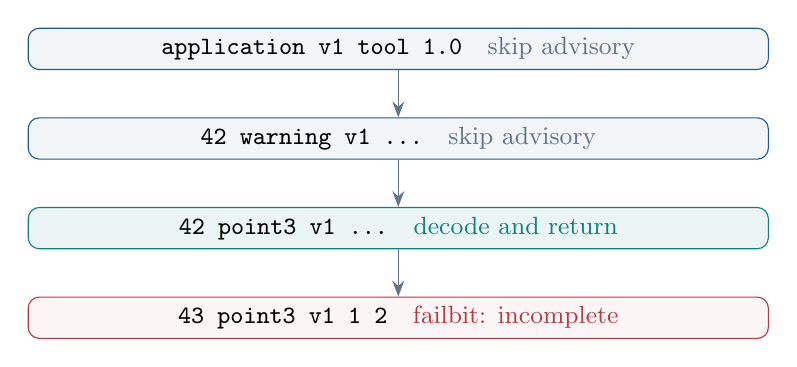
\begin{tikzpicture}[node distance=6mm]
 \node[draw=manualblue,fill=manuallight,rounded corners,minimum width=9.4cm,align=left] (a)
 {\api{application v1 tool 1.0}\quad\textcolor{manualmuted}{skip advisory}};
 \node[draw=manualblue,fill=manuallight,rounded corners,below=of a,minimum width=9.4cm,align=left] (b)
 {\api{42 warning v1 ...}\quad\textcolor{manualmuted}{skip advisory}};
 \node[draw=manualteal,fill=manualteal!8,rounded corners,below=of b,minimum width=9.4cm,align=left] (c)
 {\api{42 point3 v1 ...}\quad\textcolor{manualteal}{decode and return}};
 \node[draw=manualred,fill=manualred!5,rounded corners,below=of c,minimum width=9.4cm,align=left] (d)
 {\api{43 point3 v1 1 2}\quad\textcolor{manualred}{failbit: incomplete}};
 \draw[axis] (a)--(b); \draw[axis] (b)--(c); \draw[axis] (c)--(d);
\end{tikzpicture}
\caption{Reader calls skip advisory rows, then consume at most one required
geometry or presentation row. Malformed required data still fails strictly.}
\label{fig:tagged-reader}
\end{figure}

Malformed required rows set \api{failbit} after consuming their complete
physical row. Unknown types, unsupported required versions, missing/extra
fields, invalid tags, and invalid definitions fail. After clearing a
recoverable state, reading resumes from the next row; a reader never searches
past malformed required data. EOF and failure both return \api{nullopt}, so
inspect the stream state. CRLF and a final valid row without a newline are
accepted. Buffering and entity allocation can throw; applications needing
resource bounds must enforce their own line-size and complexity limits.

\section{Configuration and the hand-authored extension point}
\api{config.hpp} exposes semantic version strings/numbers and Git metadata,
including commit availability and dirty-state flags. Direct source includes
use the source fallback. A normal CMake build generates an updated header;
this standalone manual does not change that workflow. A repository without a
first commit can report an unborn state. Frequently used macros are:
\begin{itemize}
\item \api{NURBSPATH_VERSION_STRING}, \api{NURBSPATH_VERSION_NUMBER};
\item \api{NURBSPATH_GIT_COMMIT}, \api{NURBSPATH_GIT_COMMIT_AVAILABLE};
\item \api{NURBSPATH_GIT_DIRTY}, \api{NURBSPATH_GIT_DESCRIBE};
\item \api{NURBSPATH_CONFIG_GENERATED}.
\end{itemize}

The umbrella also includes \api{manual.hpp}, whose
\api{nurbspath::manual} namespace is an extension point for future hand-authored
functions. The current snapshot defines no algorithms there. It is distinct
from this document's top-level \api{manual/} directory.

\appendix
\chapter{Public API catalogue}\label{chap:reference}
This catalogue is generated from the public headers, using the installed
Doxygen XML extractor. It records individual callable overloads, constructors,
public member data, result records, and namespace aliases/enums. Private
members and \api{nurbspath::detail} implementation helpers are excluded.

The containing section supplies each class's template context, normally
\api{REAL}. A \api{static} member is called on the class; other members are
called on an instance. Template requirements are part of the header contract.
The compact declarations below retain the documented argument lists and
defaults; diagnostic attributes such as \api{[[nodiscard]]} can be seen in the
source headers. See the illustrated chapters for units, construction choices,
and numerical limitations. All names belong to namespace \api{nurbspath}.

\begin{manualnote}[A catalogue rather than generated implementation]
The entries show public signatures and short source comments. They do not
include function bodies. The checked-in LaTeX snapshot makes this appendix
available for a normal local TeX build even if Doxygen is unavailable later.
\api{python3 tools/generate_api.py} refreshes it without changing CMake.
\end{manualnote}
% Generated from public Doxygen XML by tools/generate_api.py.
\begingroup\setlength{\parskip}{2pt}
\Needspace{9\baselineskip}
\section{nurbspath::application\_info}
Optional output identification of the application producing a stream.
\par\noindent\begin{minipage}{\linewidth}
\begin{lstlisting}[style=apireference]
std::string name;
\end{lstlisting}
{\footnotesize Nonempty application-name token.\par}
\end{minipage}\par\vspace{1pt}
\par\noindent\begin{minipage}{\linewidth}
\begin{lstlisting}[style=apireference]
std::string version;
\end{lstlisting}
{\footnotesize Nonempty application-version token.\par}
\end{minipage}\par\vspace{1pt}
\par\noindent\begin{minipage}{\linewidth}
\begin{lstlisting}[style=apireference]
std::ostream & write(std::ostream &output) const;
\end{lstlisting}
{\footnotesize Write one optional application v1 <name> <version> output row.\par}
{\footnotesize\textit{Returns:} The destination stream, with its formatting preserved.\par}
\end{minipage}\par\vspace{1pt}
\Needspace{9\baselineskip}
\section{nurbspath::circle2}
Circle in the independent two-dimensional Cartesian world.
\par\noindent\begin{minipage}{\linewidth}
\begin{lstlisting}[style=apireference]
circle2(const point2< REAL > &center_value, REAL radius_value);
\end{lstlisting}
{\footnotesize Construct a circle.\par}
\end{minipage}\par\vspace{1pt}
\par\noindent\begin{minipage}{\linewidth}
\begin{lstlisting}[style=apireference]
const point2< REAL > & center() const noexcept;
\end{lstlisting}
{\footnotesize Get the center.\par}
{\footnotesize\textit{Returns:} Constant center reference.\par}
\end{minipage}\par\vspace{1pt}
\par\noindent\begin{minipage}{\linewidth}
\begin{lstlisting}[style=apireference]
REAL radius() const noexcept;
\end{lstlisting}
{\footnotesize Get the radius.\par}
{\footnotesize\textit{Returns:} Radius in 2D world units.\par}
\end{minipage}\par\vspace{1pt}
\par\noindent\begin{minipage}{\linewidth}
\begin{lstlisting}[style=apireference]
const point2< REAL > & get_center() const noexcept;
\end{lstlisting}
{\footnotesize Get the center.\par}
{\footnotesize\textit{Returns:} Constant reference to the center in the 2D world.\par}
\end{minipage}\par\vspace{1pt}
\par\noindent\begin{minipage}{\linewidth}
\begin{lstlisting}[style=apireference]
REAL get_radius() const noexcept;
\end{lstlisting}
{\footnotesize Get the radius.\par}
{\footnotesize\textit{Returns:} Radius in 2D world units.\par}
\end{minipage}\par\vspace{1pt}
\par\noindent\begin{minipage}{\linewidth}
\begin{lstlisting}[style=apireference]
void set_center(const point2< REAL > &center_value) noexcept;
\end{lstlisting}
{\footnotesize Replace the center while preserving the radius.\par}
\end{minipage}\par\vspace{1pt}
\par\noindent\begin{minipage}{\linewidth}
\begin{lstlisting}[style=apireference]
template <typename VECTOR>
void set_center(const VECTOR &center_value) noexcept;
\end{lstlisting}
{\footnotesize Replace the center using vector components while preserving radius.\par}
\end{minipage}\par\vspace{1pt}
\par\noindent\begin{minipage}{\linewidth}
\begin{lstlisting}[style=apireference]
void set_radius(REAL radius_value);
\end{lstlisting}
{\footnotesize Replace the radius while preserving the center.\par}
\end{minipage}\par\vspace{1pt}
\par\noindent\begin{minipage}{\linewidth}
\begin{lstlisting}[style=apireference]
void set_center_and_radius(const point2< REAL > &center_value, REAL radius_value);
\end{lstlisting}
{\footnotesize Replace the center and radius together.\par}
\end{minipage}\par\vspace{1pt}
\par\noindent\begin{minipage}{\linewidth}
\begin{lstlisting}[style=apireference]
template <typename VECTOR>
void set_center_and_radius(const VECTOR &center_value, REAL radius_value);
\end{lstlisting}
{\footnotesize Replace the center from vector components and replace the radius.\par}
\end{minipage}\par\vspace{1pt}
\par\noindent\begin{minipage}{\linewidth}
\begin{lstlisting}[style=apireference]
circle2 & operator=(const vector2< REAL > &center_value) noexcept;
\end{lstlisting}
{\footnotesize Replace the center using vector components while preserving the radius.\par}
{\footnotesize\textit{Returns:} Reference to this circle.\par}
\end{minipage}\par\vspace{1pt}
\par\noindent\begin{minipage}{\linewidth}
\begin{lstlisting}[style=apireference]
point2< REAL > point_at(REAL u) const noexcept;
\end{lstlisting}
{\footnotesize Evaluate the circle parameterization.\par}
{\footnotesize\textit{Returns:} Point on the circle in the 2D world.\par}
\end{minipage}\par\vspace{1pt}
\par\noindent\begin{minipage}{\linewidth}
\begin{lstlisting}[style=apireference]
vector2< REAL > normal_at(const point2< REAL > &point) const;
\end{lstlisting}
{\footnotesize Compute the outward radial unit normal at a point.\par}
{\footnotesize\textit{Returns:} Outward unit direction after radial projection.\par}
\end{minipage}\par\vspace{1pt}
\par\noindent\begin{minipage}{\linewidth}
\begin{lstlisting}[style=apireference]
REAL parameter_of(const point2< REAL > &point, REAL tolerance=REAL(0)) const;
\end{lstlisting}
{\footnotesize Recover the angular parameter by radial projection.\par}
{\footnotesize\textit{Returns:} Counterclockwise angle in [0,2*pi).\par}
\end{minipage}\par\vspace{1pt}
\Needspace{9\baselineskip}
\section{nurbspath::diagnostic\_message3}
Optional output diagnostic anchored at a position in the 3D world.
\par\noindent\begin{minipage}{\linewidth}
\begin{lstlisting}[style=apireference]
diagnostic_level level = diagnostic_level::information;
\end{lstlisting}
{\footnotesize Output severity.\par}
\end{minipage}\par\vspace{1pt}
\par\noindent\begin{minipage}{\linewidth}
\begin{lstlisting}[style=apireference]
point3< REAL > position {};
\end{lstlisting}
{\footnotesize Finite world-space position of the annotation.\par}
\end{minipage}\par\vspace{1pt}
\par\noindent\begin{minipage}{\linewidth}
\begin{lstlisting}[style=apireference]
REAL size = REAL(12);
\end{lstlisting}
{\footnotesize Positive text size in consumer display units.\par}
\end{minipage}\par\vspace{1pt}
\par\noindent\begin{minipage}{\linewidth}
\begin{lstlisting}[style=apireference]
std::string value;
\end{lstlisting}
{\footnotesize Text, optionally containing escaped line breaks.\par}
\end{minipage}\par\vspace{1pt}
\par\noindent\begin{minipage}{\linewidth}
\begin{lstlisting}[style=apireference]
std::ostream & tag_write(std::size_t tag, std::ostream &output) const;
\end{lstlisting}
{\footnotesize Write an optional positioned warning, information, or error row.\par}
{\footnotesize\textit{Returns:} The destination stream, with its formatting preserved.\par}
\end{minipage}\par\vspace{1pt}
\Needspace{9\baselineskip}
\section{nurbspath::intersection2}
2D contact with parameters of both participating entities.
\par\noindent\begin{minipage}{\linewidth}
\begin{lstlisting}[style=apireference]
point2< REAL > point;
\end{lstlisting}
{\footnotesize Contact point in the independent 2D world.\par}
\end{minipage}\par\vspace{1pt}
\par\noindent\begin{minipage}{\linewidth}
\begin{lstlisting}[style=apireference]
REAL s = REAL(0);
\end{lstlisting}
{\footnotesize Ray or spline parameter.\par}
\end{minipage}\par\vspace{1pt}
\par\noindent\begin{minipage}{\linewidth}
\begin{lstlisting}[style=apireference]
REAL u = REAL(0);
\end{lstlisting}
{\footnotesize Circle angle in [0,2*pi).\par}
\end{minipage}\par\vspace{1pt}
\par\noindent\begin{minipage}{\linewidth}
\begin{lstlisting}[style=apireference]
REAL residual = REAL(0);
\end{lstlisting}
{\footnotesize Absolute 2D circle residual after refinement.\par}
\end{minipage}\par\vspace{1pt}
\Needspace{9\baselineskip}
\section{nurbspath::intersection3}
World-space contact with parameters of both participating entities.
\par\noindent\begin{minipage}{\linewidth}
\begin{lstlisting}[style=apireference]
point3< REAL > point;
\end{lstlisting}
{\footnotesize Contact point in world coordinates.\par}
\end{minipage}\par\vspace{1pt}
\par\noindent\begin{minipage}{\linewidth}
\begin{lstlisting}[style=apireference]
REAL s = REAL(0);
\end{lstlisting}
{\footnotesize Ray or spline parameter.\par}
\end{minipage}\par\vspace{1pt}
\par\noindent\begin{minipage}{\linewidth}
\begin{lstlisting}[style=apireference]
REAL u = REAL(0);
\end{lstlisting}
{\footnotesize Sphere or plane u parameter.\par}
\end{minipage}\par\vspace{1pt}
\par\noindent\begin{minipage}{\linewidth}
\begin{lstlisting}[style=apireference]
REAL v = REAL(0);
\end{lstlisting}
{\footnotesize Sphere or plane v parameter.\par}
\end{minipage}\par\vspace{1pt}
\par\noindent\begin{minipage}{\linewidth}
\begin{lstlisting}[style=apireference]
REAL residual = REAL(0);
\end{lstlisting}
{\footnotesize Absolute surface residual after refinement.\par}
\end{minipage}\par\vspace{1pt}
\Needspace{9\baselineskip}
\section{nurbspath::intersection\_result2}
Complete result of one two-dimensional intersection query.
\par\noindent\begin{minipage}{\linewidth}
\begin{lstlisting}[style=apireference]
intersection_kind kind = intersection_kind::none;
\end{lstlisting}
{\footnotesize Set classification.\par}
\end{minipage}\par\vspace{1pt}
\par\noindent\begin{minipage}{\linewidth}
\begin{lstlisting}[style=apireference]
std::vector< intersection2< REAL > > points;
\end{lstlisting}
{\footnotesize Isolated contacts sorted by s.\par}
\end{minipage}\par\vspace{1pt}
\par\noindent\begin{minipage}{\linewidth}
\begin{lstlisting}[style=apireference]
bool has_intersection() const noexcept;
\end{lstlisting}
{\footnotesize Test for isolated or coincident contact.\par}
{\footnotesize\textit{Returns:} True unless kind is none.\par}
\end{minipage}\par\vspace{1pt}
\par\noindent\begin{minipage}{\linewidth}
\begin{lstlisting}[style=apireference]
bool is_coincident() const noexcept;
\end{lstlisting}
{\footnotesize Test for continuous overlap.\par}
{\footnotesize\textit{Returns:} True when kind is coincident.\par}
\end{minipage}\par\vspace{1pt}
\Needspace{9\baselineskip}
\section{nurbspath::intersection\_result3}
Complete result of one intersection query.
\par\noindent\begin{minipage}{\linewidth}
\begin{lstlisting}[style=apireference]
intersection_kind kind = intersection_kind::none;
\end{lstlisting}
{\footnotesize Set classification.\par}
\end{minipage}\par\vspace{1pt}
\par\noindent\begin{minipage}{\linewidth}
\begin{lstlisting}[style=apireference]
std::vector< intersection3< REAL > > points;
\end{lstlisting}
{\footnotesize Isolated contacts sorted by s.\par}
\end{minipage}\par\vspace{1pt}
\par\noindent\begin{minipage}{\linewidth}
\begin{lstlisting}[style=apireference]
bool has_intersection() const noexcept;
\end{lstlisting}
{\footnotesize Test for any isolated or coincident contact.\par}
{\footnotesize\textit{Returns:} True unless kind is none.\par}
\end{minipage}\par\vspace{1pt}
\par\noindent\begin{minipage}{\linewidth}
\begin{lstlisting}[style=apireference]
bool is_coincident() const noexcept;
\end{lstlisting}
{\footnotesize Test for continuous overlap.\par}
{\footnotesize\textit{Returns:} True when kind is coincident.\par}
\end{minipage}\par\vspace{1pt}
\Needspace{9\baselineskip}
\section{nurbspath::line\_color}
Optional normalized RGBA line color associated with an application tag.
\par\noindent\begin{minipage}{\linewidth}
\begin{lstlisting}[style=apireference]
REAL red = REAL(0);
\end{lstlisting}
{\footnotesize Normalized red component in [0, 1].\par}
\end{minipage}\par\vspace{1pt}
\par\noindent\begin{minipage}{\linewidth}
\begin{lstlisting}[style=apireference]
REAL green = REAL(0);
\end{lstlisting}
{\footnotesize Normalized green component in [0, 1].\par}
\end{minipage}\par\vspace{1pt}
\par\noindent\begin{minipage}{\linewidth}
\begin{lstlisting}[style=apireference]
REAL blue = REAL(0);
\end{lstlisting}
{\footnotesize Normalized blue component in [0, 1].\par}
\end{minipage}\par\vspace{1pt}
\par\noindent\begin{minipage}{\linewidth}
\begin{lstlisting}[style=apireference]
REAL alpha = REAL(1);
\end{lstlisting}
{\footnotesize Normalized opacity in [0, 1].\par}
\end{minipage}\par\vspace{1pt}
\par\noindent\begin{minipage}{\linewidth}
\begin{lstlisting}[style=apireference]
std::ostream & tag_write(std::size_t tag, std::ostream &output) const;
\end{lstlisting}
{\footnotesize Write one version-1 linecolor row without changing stream format.\par}
{\footnotesize\textit{Returns:} The destination stream.\par}
\end{minipage}\par\vspace{1pt}
\par\noindent\begin{minipage}{\linewidth}
\begin{lstlisting}[style=apireference]
static std::optional< tagged_read_result< line_color > > tag_read(std::istream &input);
\end{lstlisting}
{\footnotesize Read one linecolor v1 row and allocate a validated color. Advisory application and diagnostic rows are skipped without decoding.\par}
{\footnotesize\textit{Returns:} Preserved tag and non-null color owner, or nullopt on EOF/failure. Malformed rows set failbit and consume only their own physical row.\par}
\end{minipage}\par\vspace{1pt}
\Needspace{9\baselineskip}
\section{nurbspath::line\_font}
Optional line width and repeating dash lengths for tagged line elements.
\par\noindent\begin{minipage}{\linewidth}
\begin{lstlisting}[style=apireference]
REAL width = REAL(1);
\end{lstlisting}
{\footnotesize Positive stroke width in consumer display units.\par}
\end{minipage}\par\vspace{1pt}
\par\noindent\begin{minipage}{\linewidth}
\begin{lstlisting}[style=apireference]
REAL on = REAL(0);
\end{lstlisting}
{\footnotesize Visible dash length; zero with off for a solid line.\par}
\end{minipage}\par\vspace{1pt}
\par\noindent\begin{minipage}{\linewidth}
\begin{lstlisting}[style=apireference]
REAL off = REAL(0);
\end{lstlisting}
{\footnotesize Gap length; zero with on for a solid line.\par}
\end{minipage}\par\vspace{1pt}
\par\noindent\begin{minipage}{\linewidth}
\begin{lstlisting}[style=apireference]
std::ostream & tag_write(std::size_t tag, std::ostream &output) const;
\end{lstlisting}
{\footnotesize Write one version-1 linefont row without changing stream format.\par}
{\footnotesize\textit{Returns:} The destination stream.\par}
\end{minipage}\par\vspace{1pt}
\par\noindent\begin{minipage}{\linewidth}
\begin{lstlisting}[style=apireference]
static std::optional< tagged_read_result< line_font > > tag_read(std::istream &input);
\end{lstlisting}
{\footnotesize Read one linefont v1 row and allocate a validated line font. Advisory application and diagnostic rows are skipped without decoding.\par}
{\footnotesize\textit{Returns:} Preserved tag and non-null font owner, or nullopt on EOF/failure. Malformed rows set failbit and consume only their own physical row.\par}
\end{minipage}\par\vspace{1pt}
\Needspace{9\baselineskip}
\section{nurbspath::numerical\_settings}
Controls iterative and sampled numerical algorithms.
\par\noindent\begin{minipage}{\linewidth}
\begin{lstlisting}[style=apireference]
REAL residual_tolerance = REAL(1e-8);
\end{lstlisting}
{\footnotesize Accepted absolute function residual.\par}
\end{minipage}\par\vspace{1pt}
\par\noindent\begin{minipage}{\linewidth}
\begin{lstlisting}[style=apireference]
REAL parameter_tolerance = REAL(1e-10);
\end{lstlisting}
{\footnotesize Accepted parameter interval width.\par}
\end{minipage}\par\vspace{1pt}
\par\noindent\begin{minipage}{\linewidth}
\begin{lstlisting}[style=apireference]
std::size_t max_iterations = 100;
\end{lstlisting}
{\footnotesize Maximum refinement iterations.\par}
\end{minipage}\par\vspace{1pt}
\par\noindent\begin{minipage}{\linewidth}
\begin{lstlisting}[style=apireference]
std::size_t sample_count = 256;
\end{lstlisting}
{\footnotesize Number of initial uniform intervals.\par}
\end{minipage}\par\vspace{1pt}
\par\noindent\begin{minipage}{\linewidth}
\begin{lstlisting}[style=apireference]
void validate() const;
\end{lstlisting}
{\footnotesize Validate all numerical controls.\par}
\end{minipage}\par\vspace{1pt}
\Needspace{9\baselineskip}
\section{nurbspath::nurbs\_arr\_spline2}
Self-contained 2D NURBS curve backed by one public scalar valarray.
\par\noindent\begin{minipage}{\linewidth}
\begin{lstlisting}[style=apireference]
using real_t = REAL;
\end{lstlisting}
{\footnotesize Floating-point scalar stored by this spline.\par}
\end{minipage}\par\vspace{1pt}
\par\noindent\begin{minipage}{\linewidth}
\begin{lstlisting}[style=apireference]
using parameter_index_range = std::ranges::iota_view< std::size_t, std::size_t >;
\end{lstlisting}
{\footnotesize Allocation-free range of flattened indices into parameters.\par}
\end{minipage}\par\vspace{1pt}
\par\noindent\begin{minipage}{\linewidth}
\begin{lstlisting}[style=apireference]
std::valarray< REAL > parameters;
\end{lstlisting}
{\footnotesize Flattened control coordinates, weights, and knots.\par}
\end{minipage}\par\vspace{1pt}
\par\noindent\begin{minipage}{\linewidth}
\begin{lstlisting}[style=apireference]
nurbs_arr_spline2(const point2< REAL > &start, const point2< REAL > &end, std::size_t control_point_count, std::size_t degree, REAL tolerance);
\end{lstlisting}
{\footnotesize Construct a standard open 2D spline with explicit tolerance.\par}
\end{minipage}\par\vspace{1pt}
\par\noindent\begin{minipage}{\linewidth}
\begin{lstlisting}[style=apireference]
template <std::same_as< bool > CLOSED = bool>
nurbs_arr_spline2(const point2< REAL > &start, const point2< REAL > &end, std::size_t control_point_count, std::size_t degree, CLOSED closed=false, REAL tolerance=REAL(64) *std::numeric_limits< REAL >::epsilon());
\end{lstlisting}
{\footnotesize Construct a standard open or closed spline between two points.\par}
\end{minipage}\par\vspace{1pt}
\par\noindent\begin{minipage}{\linewidth}
\begin{lstlisting}[style=apireference]
nurbs_arr_spline2(std::valarray< REAL > values, std::size_t degree, REAL tolerance=REAL(64) *std::numeric_limits< REAL >::epsilon());
\end{lstlisting}
{\footnotesize Construct an open array-backed spline from flattened parameters.\par}
\end{minipage}\par\vspace{1pt}
\par\noindent\begin{minipage}{\linewidth}
\begin{lstlisting}[style=apireference]
template <std::same_as< bool > CLOSED>
nurbs_arr_spline2(std::valarray< REAL > values, std::size_t degree, CLOSED closed, REAL tolerance=REAL(64) *std::numeric_limits< REAL >::epsilon());
\end{lstlisting}
{\footnotesize Construct an open or closed spline from flattened parameters.\par}
\end{minipage}\par\vspace{1pt}
\par\noindent\begin{minipage}{\linewidth}
\begin{lstlisting}[style=apireference]
nurbs_arr_spline2(std::vector< point2< REAL > > control_points, std::vector< REAL > weights, std::vector< REAL > knots, std::size_t degree, REAL tolerance=REAL(64) *std::numeric_limits< REAL >::epsilon());
\end{lstlisting}
{\footnotesize Construct an open array-backed spline from component vectors.\par}
\end{minipage}\par\vspace{1pt}
\par\noindent\begin{minipage}{\linewidth}
\begin{lstlisting}[style=apireference]
template <std::same_as< bool > CLOSED>
nurbs_arr_spline2(std::vector< point2< REAL > > control_points, std::vector< REAL > weights, std::vector< REAL > knots, std::size_t degree, CLOSED closed, REAL tolerance=REAL(64) *std::numeric_limits< REAL >::epsilon());
\end{lstlisting}
{\footnotesize Construct an open or closed spline from component vectors.\par}
\end{minipage}\par\vspace{1pt}
\par\noindent\begin{minipage}{\linewidth}
\begin{lstlisting}[style=apireference]
nurbs_arr_spline2(const nurbs_spline2< REAL > &spline);
\end{lstlisting}
{\footnotesize Copy an ordinary 2D NURBS spline into flattened storage.\par}
\end{minipage}\par\vspace{1pt}
\par\noindent\begin{minipage}{\linewidth}
\begin{lstlisting}[style=apireference]
std::size_t degree() const noexcept;
\end{lstlisting}
{\footnotesize Get the polynomial degree.\par}
{\footnotesize\textit{Returns:} Positive spline degree.\par}
\end{minipage}\par\vspace{1pt}
\par\noindent\begin{minipage}{\linewidth}
\begin{lstlisting}[style=apireference]
REAL tolerance() const noexcept;
\end{lstlisting}
{\footnotesize Get the definition and parameter-boundary tolerance.\par}
{\footnotesize\textit{Returns:} Current tolerance.\par}
\end{minipage}\par\vspace{1pt}
\par\noindent\begin{minipage}{\linewidth}
\begin{lstlisting}[style=apireference]
bool is_closed() const noexcept;
\end{lstlisting}
{\footnotesize Report whether the spline requires a closed seam.\par}
{\footnotesize\textit{Returns:} True when active-domain endpoints must coincide.\par}
\end{minipage}\par\vspace{1pt}
\par\noindent\begin{minipage}{\linewidth}
\begin{lstlisting}[style=apireference]
std::size_t number_of_parameters() const noexcept;
\end{lstlisting}
{\footnotesize Get the number of flattened scalar parameters.\par}
{\footnotesize\textit{Returns:} Current public array size, including malformed layouts.\par}
\end{minipage}\par\vspace{1pt}
\par\noindent\begin{minipage}{\linewidth}
\begin{lstlisting}[style=apireference]
std::size_t control_point_count() const;
\end{lstlisting}
{\footnotesize Derive the control-point count from the current array layout.\par}
{\footnotesize\textit{Returns:} Number of represented control points.\par}
\end{minipage}\par\vspace{1pt}
\par\noindent\begin{minipage}{\linewidth}
\begin{lstlisting}[style=apireference]
std::size_t knot_count() const;
\end{lstlisting}
{\footnotesize Derive the knot count from the current array layout.\par}
{\footnotesize\textit{Returns:} Number of represented knots.\par}
\end{minipage}\par\vspace{1pt}
\par\noindent\begin{minipage}{\linewidth}
\begin{lstlisting}[style=apireference]
std::size_t weight_count() const;
\end{lstlisting}
{\footnotesize Derive the weight count from the current array layout.\par}
{\footnotesize\textit{Returns:} Number of represented weights, equal to the control-point count.\par}
\end{minipage}\par\vspace{1pt}
\par\noindent\begin{minipage}{\linewidth}
\begin{lstlisting}[style=apireference]
parameter_index_range get_control_point_count_range() const;
\end{lstlisting}
{\footnotesize Get the flattened indices occupied by control-point coordinates.\par}
{\footnotesize\textit{Returns:} Iterable scalar-index range [0, 2 * control\_point\_count()).\par}
\end{minipage}\par\vspace{1pt}
\par\noindent\begin{minipage}{\linewidth}
\begin{lstlisting}[style=apireference]
parameter_index_range get_weight_count_range() const;
\end{lstlisting}
{\footnotesize Get the flattened indices occupied by rational weights.\par}
{\footnotesize\textit{Returns:} Iterable scalar-index range [2 * C, 3 * C), where C is the control-point count.\par}
\end{minipage}\par\vspace{1pt}
\par\noindent\begin{minipage}{\linewidth}
\begin{lstlisting}[style=apireference]
parameter_index_range get_knot_count_range() const;
\end{lstlisting}
{\footnotesize Get the flattened indices occupied by knots.\par}
{\footnotesize\textit{Returns:} Iterable scalar-index range [3 * C, parameters.size()), where C is the control-point count.\par}
\end{minipage}\par\vspace{1pt}
\par\noindent\begin{minipage}{\linewidth}
\begin{lstlisting}[style=apireference]
std::vector< point2< REAL > > get_control_points() const;
\end{lstlisting}
{\footnotesize Get all control points as detached point values.\par}
{\footnotesize\textit{Returns:} Control points reconstructed in index order.\par}
\end{minipage}\par\vspace{1pt}
\par\noindent\begin{minipage}{\linewidth}
\begin{lstlisting}[style=apireference]
std::vector< REAL > get_weights() const;
\end{lstlisting}
{\footnotesize Get all weights as a detached vector.\par}
{\footnotesize\textit{Returns:} Weights copied in index order.\par}
\end{minipage}\par\vspace{1pt}
\par\noindent\begin{minipage}{\linewidth}
\begin{lstlisting}[style=apireference]
std::vector< REAL > get_knots() const;
\end{lstlisting}
{\footnotesize Get all knots as a detached vector.\par}
{\footnotesize\textit{Returns:} Knots copied in index order.\par}
\end{minipage}\par\vspace{1pt}
\par\noindent\begin{minipage}{\linewidth}
\begin{lstlisting}[style=apireference]
point2< REAL > get_control_point(std::size_t index) const;
\end{lstlisting}
{\footnotesize Get one control point by index.\par}
{\footnotesize\textit{Returns:} Point reconstructed by value from two adjacent scalars.\par}
\end{minipage}\par\vspace{1pt}
\par\noindent\begin{minipage}{\linewidth}
\begin{lstlisting}[style=apireference]
REAL get_weight(std::size_t index) const;
\end{lstlisting}
{\footnotesize Get one rational weight by index.\par}
{\footnotesize\textit{Returns:} Selected weight value.\par}
\end{minipage}\par\vspace{1pt}
\par\noindent\begin{minipage}{\linewidth}
\begin{lstlisting}[style=apireference]
REAL get_knot(std::size_t index) const;
\end{lstlisting}
{\footnotesize Get one knot by index.\par}
{\footnotesize\textit{Returns:} Selected knot value.\par}
\end{minipage}\par\vspace{1pt}
\par\noindent\begin{minipage}{\linewidth}
\begin{lstlisting}[style=apireference]
REAL get_parameter(std::size_t index) const;
\end{lstlisting}
{\footnotesize Get one scalar by its flattened index.\par}
{\footnotesize\textit{Returns:} Selected scalar value.\par}
\end{minipage}\par\vspace{1pt}
\par\noindent\begin{minipage}{\linewidth}
\begin{lstlisting}[style=apireference]
std::string parameter_name(std::size_t index) const;
\end{lstlisting}
{\footnotesize Get the descriptive name of one flattened scalar.\par}
{\footnotesize\textit{Returns:} A P[i].x, P[i].y, W[i], or K[i] name.\par}
\end{minipage}\par\vspace{1pt}
\par\noindent\begin{minipage}{\linewidth}
\begin{lstlisting}[style=apireference]
void validate() const;
\end{lstlisting}
{\footnotesize Validate the current public array and all typed metadata.\par}
\end{minipage}\par\vspace{1pt}
\par\noindent\begin{minipage}{\linewidth}
\begin{lstlisting}[style=apireference]
void set_parameters(std::valarray< REAL > values);
\end{lstlisting}
{\footnotesize Atomically validate and replace the complete public scalar array.\par}
\end{minipage}\par\vspace{1pt}
\par\noindent\begin{minipage}{\linewidth}
\begin{lstlisting}[style=apireference]
void set_parameters(const REAL *values);
\end{lstlisting}
{\footnotesize Atomically copy and replace the complete public scalar array.\par}
\end{minipage}\par\vspace{1pt}
\par\noindent\begin{minipage}{\linewidth}
\begin{lstlisting}[style=apireference]
bool set_parameter(std::size_t index, REAL value);
\end{lstlisting}
{\footnotesize Atomically validate and replace one flattened scalar.\par}
{\footnotesize\textit{Returns:} True when the candidate was valid and committed; false for an out-of-range index, malformed current shape, or a rejected value.\par}
\end{minipage}\par\vspace{1pt}
\par\noindent\begin{minipage}{\linewidth}
\begin{lstlisting}[style=apireference]
void set_control_point(std::size_t index, const point2< REAL > &point);
\end{lstlisting}
{\footnotesize Atomically replace one control point.\par}
\end{minipage}\par\vspace{1pt}
\par\noindent\begin{minipage}{\linewidth}
\begin{lstlisting}[style=apireference]
void set_weight(std::size_t index, REAL value);
\end{lstlisting}
{\footnotesize Atomically replace one rational weight.\par}
\end{minipage}\par\vspace{1pt}
\par\noindent\begin{minipage}{\linewidth}
\begin{lstlisting}[style=apireference]
void set_knot(std::size_t index, REAL value);
\end{lstlisting}
{\footnotesize Atomically replace one knot.\par}
\end{minipage}\par\vspace{1pt}
\par\noindent\begin{minipage}{\linewidth}
\begin{lstlisting}[style=apireference]
void set_control_points(std::vector< point2< REAL > > control_points);
\end{lstlisting}
{\footnotesize Atomically replace all control points while retaining other data.\par}
\end{minipage}\par\vspace{1pt}
\par\noindent\begin{minipage}{\linewidth}
\begin{lstlisting}[style=apireference]
void set_weights(std::vector< REAL > values);
\end{lstlisting}
{\footnotesize Atomically replace all weights while retaining other data.\par}
\end{minipage}\par\vspace{1pt}
\par\noindent\begin{minipage}{\linewidth}
\begin{lstlisting}[style=apireference]
void set_knots(std::vector< REAL > values);
\end{lstlisting}
{\footnotesize Atomically replace all knots while retaining other data.\par}
\end{minipage}\par\vspace{1pt}
\par\noindent\begin{minipage}{\linewidth}
\begin{lstlisting}[style=apireference]
void set_standard_knots(REAL s_end);
\end{lstlisting}
{\footnotesize Set standard open-clamped knots on [0, s\_end].\par}
\end{minipage}\par\vspace{1pt}
\par\noindent\begin{minipage}{\linewidth}
\begin{lstlisting}[style=apireference]
void set_standard_knots(REAL s_start, REAL s_end);
\end{lstlisting}
{\footnotesize Set standard open-clamped knots on [s\_start, s\_end].\par}
\end{minipage}\par\vspace{1pt}
\par\noindent\begin{minipage}{\linewidth}
\begin{lstlisting}[style=apireference]
void set_tolerance(REAL value);
\end{lstlisting}
{\footnotesize Atomically replace the validation tolerance.\par}
\end{minipage}\par\vspace{1pt}
\par\noindent\begin{minipage}{\linewidth}
\begin{lstlisting}[style=apireference]
void set_closed(bool value);
\end{lstlisting}
{\footnotesize Atomically change the closed-seam requirement.\par}
\end{minipage}\par\vspace{1pt}
\par\noindent\begin{minipage}{\linewidth}
\begin{lstlisting}[style=apireference]
void set_definition(std::vector< point2< REAL > > control_points, std::vector< REAL > weights, std::vector< REAL > knots, bool closed, REAL tolerance);
\end{lstlisting}
{\footnotesize Atomically replace all numeric components and mutable metadata.\par}
\end{minipage}\par\vspace{1pt}
\par\noindent\begin{minipage}{\linewidth}
\begin{lstlisting}[style=apireference]
REAL s_min() const;
\end{lstlisting}
{\footnotesize Get the lower active parameter bound from the current knot data.\par}
{\footnotesize\textit{Returns:} Minimum valid native s.\par}
\end{minipage}\par\vspace{1pt}
\par\noindent\begin{minipage}{\linewidth}
\begin{lstlisting}[style=apireference]
REAL s_max() const;
\end{lstlisting}
{\footnotesize Get the upper active parameter bound from the current knot data.\par}
{\footnotesize\textit{Returns:} Maximum valid native s.\par}
\end{minipage}\par\vspace{1pt}
\par\noindent\begin{minipage}{\linewidth}
\begin{lstlisting}[style=apireference]
point2< REAL > get_start() const;
\end{lstlisting}
{\footnotesize Evaluate the current point at the active-domain start.\par}
{\footnotesize\textit{Returns:} Start point derived on demand from public storage.\par}
\end{minipage}\par\vspace{1pt}
\par\noindent\begin{minipage}{\linewidth}
\begin{lstlisting}[style=apireference]
point2< REAL > get_end() const;
\end{lstlisting}
{\footnotesize Evaluate the current point at the active-domain end.\par}
{\footnotesize\textit{Returns:} End point derived on demand from public storage.\par}
\end{minipage}\par\vspace{1pt}
\par\noindent\begin{minipage}{\linewidth}
\begin{lstlisting}[style=apireference]
spline_derivatives2< REAL > derivatives_at(REAL s) const;
\end{lstlisting}
{\footnotesize Evaluate position and the first two analytic derivatives.\par}
{\footnotesize\textit{Returns:} Position, first derivative, and second derivative in 2D.\par}
\end{minipage}\par\vspace{1pt}
\par\noindent\begin{minipage}{\linewidth}
\begin{lstlisting}[style=apireference]
point2< REAL > evaluate(REAL s) const;
\end{lstlisting}
{\footnotesize Evaluate the curve position.\par}
{\footnotesize\textit{Returns:} Curve point in the independent 2D world.\par}
\end{minipage}\par\vspace{1pt}
\par\noindent\begin{minipage}{\linewidth}
\begin{lstlisting}[style=apireference]
point2< REAL > point_at(REAL s) const;
\end{lstlisting}
{\footnotesize Evaluate the curve position.\par}
{\footnotesize\textit{Returns:} Curve point in the independent 2D world.\par}
\end{minipage}\par\vspace{1pt}
\par\noindent\begin{minipage}{\linewidth}
\begin{lstlisting}[style=apireference]
vector2< REAL > first_derivative(REAL s) const;
\end{lstlisting}
{\footnotesize Evaluate the first analytic derivative.\par}
{\footnotesize\textit{Returns:} First derivative with respect to native s.\par}
\end{minipage}\par\vspace{1pt}
\par\noindent\begin{minipage}{\linewidth}
\begin{lstlisting}[style=apireference]
vector2< REAL > second_derivative(REAL s) const;
\end{lstlisting}
{\footnotesize Evaluate the second analytic derivative.\par}
{\footnotesize\textit{Returns:} Second derivative with respect to native s.\par}
\end{minipage}\par\vspace{1pt}
\par\noindent\begin{minipage}{\linewidth}
\begin{lstlisting}[style=apireference]
vector2< REAL > third_derivative(REAL s) const;
\end{lstlisting}
{\footnotesize Evaluate the third analytic rational derivative.\par}
{\footnotesize\textit{Returns:} Third derivative with respect to native s.\par}
\end{minipage}\par\vspace{1pt}
\par\noindent\begin{minipage}{\linewidth}
\begin{lstlisting}[style=apireference]
vector2< REAL > tangent(REAL s, REAL tolerance=vector2< REAL >::default_tolerance()) const;
\end{lstlisting}
{\footnotesize Evaluate a unit tangent.\par}
{\footnotesize\textit{Returns:} Normalized first derivative.\par}
\end{minipage}\par\vspace{1pt}
\par\noindent\begin{minipage}{\linewidth}
\begin{lstlisting}[style=apireference]
REAL curvature(REAL s, REAL tangent_tolerance=vector2< REAL >::default_tolerance()) const;
\end{lstlisting}
{\footnotesize Evaluate unsigned geometric curvature in the 2D world.\par}
{\footnotesize\textit{Returns:} Nonnegative curvature magnitude in inverse 2D world units.\par}
\end{minipage}\par\vspace{1pt}
\par\noindent\begin{minipage}{\linewidth}
\begin{lstlisting}[style=apireference]
REAL get_polygon_length() const;
\end{lstlisting}
{\footnotesize Get the total length of the current 2D control polygon.\par}
{\footnotesize\textit{Returns:} Control-polygon length in 2D world units.\par}
\end{minipage}\par\vspace{1pt}
\par\noindent\begin{minipage}{\linewidth}
\begin{lstlisting}[style=apireference]
REAL approximate_arc_length(std::size_t segment_count=512) const;
\end{lstlisting}
{\footnotesize Estimate arc length using a uniform-native-s polyline.\par}
{\footnotesize\textit{Returns:} Approximate length in 2D world units.\par}
\end{minipage}\par\vspace{1pt}
\par\noindent\begin{minipage}{\linewidth}
\begin{lstlisting}[style=apireference]
void adopt_to_points(const std::vector< point2< REAL > > &samples, const std::vector< REAL > &arc_length_parameters, std::size_t requested_degree=3, REAL tolerance=REAL(1e-10));
\end{lstlisting}
{\footnotesize Replace this curve with an open interpolant through samples.\par}
\end{minipage}\par\vspace{1pt}
\par\noindent\begin{minipage}{\linewidth}
\begin{lstlisting}[style=apireference]
void adopt_to_points(const std::vector< point2< REAL > > &samples, const std::vector< REAL > &arc_length_parameters, std::size_t requested_degree, bool closed, REAL tolerance=REAL(1e-10));
\end{lstlisting}
{\footnotesize Replace this curve with an open or closed interpolant.\par}
\end{minipage}\par\vspace{1pt}
\par\noindent\begin{minipage}{\linewidth}
\begin{lstlisting}[style=apireference]
nurbs_spline2< REAL > to_nurbs_spline() const;
\end{lstlisting}
{\footnotesize Convert to the ordinary vector-backed 2D NURBS type.\par}
{\footnotesize\textit{Returns:} Valid ordinary spline with identical geometry and metadata.\par}
\end{minipage}\par\vspace{1pt}
\par\noindent\begin{minipage}{\linewidth}
\begin{lstlisting}[style=apireference]
static nurbs_arr_spline2 interpolate(const std::vector< point2< REAL > > &samples, const std::vector< REAL > &arc_length_parameters, std::size_t requested_degree=3, REAL tolerance=REAL(1e-10));
\end{lstlisting}
{\footnotesize Build an open unit-weight spline interpolating measured samples.\par}
{\footnotesize\textit{Returns:} Array-backed interpolating curve.\par}
\end{minipage}\par\vspace{1pt}
\par\noindent\begin{minipage}{\linewidth}
\begin{lstlisting}[style=apireference]
static nurbs_arr_spline2 interpolate(const std::vector< point2< REAL > > &samples, const std::vector< REAL > &arc_length_parameters, std::size_t requested_degree, bool closed, REAL tolerance=REAL(1e-10));
\end{lstlisting}
{\footnotesize Build an open or closed unit-weight interpolating spline.\par}
{\footnotesize\textit{Returns:} Array-backed interpolating curve.\par}
\end{minipage}\par\vspace{1pt}
\Needspace{9\baselineskip}
\section{nurbspath::nurbs\_arr\_spline3}
Self-contained 3D NURBS curve backed by one public scalar valarray.
\par\noindent\begin{minipage}{\linewidth}
\begin{lstlisting}[style=apireference]
using real_t = REAL;
\end{lstlisting}
{\footnotesize Scalar type stored by this spline.\par}
\end{minipage}\par\vspace{1pt}
\par\noindent\begin{minipage}{\linewidth}
\begin{lstlisting}[style=apireference]
using parameter_index_range = std::ranges::iota_view< std::size_t, std::size_t >;
\end{lstlisting}
{\footnotesize Allocation-free range of flattened indices into parameters.\par}
\end{minipage}\par\vspace{1pt}
\par\noindent\begin{minipage}{\linewidth}
\begin{lstlisting}[style=apireference]
std::valarray< REAL > parameters;
\end{lstlisting}
{\footnotesize Flattened control-coordinate, weight, and knot storage.\par}
\end{minipage}\par\vspace{1pt}
\par\noindent\begin{minipage}{\linewidth}
\begin{lstlisting}[style=apireference]
nurbs_arr_spline3(const point3< REAL > &start, const point3< REAL > &end, std::size_t control_point_count, std::size_t degree, REAL tolerance);
\end{lstlisting}
{\footnotesize Construct a standard open 3D spline with explicit tolerance.\par}
\end{minipage}\par\vspace{1pt}
\par\noindent\begin{minipage}{\linewidth}
\begin{lstlisting}[style=apireference]
template <std::same_as< bool > CLOSED = bool>
nurbs_arr_spline3(const point3< REAL > &start, const point3< REAL > &end, std::size_t control_point_count, std::size_t degree, CLOSED closed=false, REAL tolerance=REAL(64) *std::numeric_limits< REAL >::epsilon());
\end{lstlisting}
{\footnotesize Construct a standard open or closed spline between two 3D points.\par}
\end{minipage}\par\vspace{1pt}
\par\noindent\begin{minipage}{\linewidth}
\begin{lstlisting}[style=apireference]
nurbs_arr_spline3(std::valarray< REAL > parameter_values, std::size_t degree, REAL tolerance=REAL(64) *std::numeric_limits< REAL >::epsilon());
\end{lstlisting}
{\footnotesize Construct an open array spline from flattened scalar parameters.\par}
\end{minipage}\par\vspace{1pt}
\par\noindent\begin{minipage}{\linewidth}
\begin{lstlisting}[style=apireference]
template <std::same_as< bool > CLOSED>
nurbs_arr_spline3(std::valarray< REAL > parameter_values, std::size_t degree, CLOSED closed, REAL tolerance=REAL(64) *std::numeric_limits< REAL >::epsilon());
\end{lstlisting}
{\footnotesize Construct an open or closed array spline from flattened scalars.\par}
\end{minipage}\par\vspace{1pt}
\par\noindent\begin{minipage}{\linewidth}
\begin{lstlisting}[style=apireference]
nurbs_arr_spline3(std::vector< point3< REAL > > control_points, std::vector< REAL > weights, std::vector< REAL > knots, std::size_t degree, REAL tolerance=REAL(64) *std::numeric_limits< REAL >::epsilon());
\end{lstlisting}
{\footnotesize Construct an open array spline from ordinary vector collections.\par}
\end{minipage}\par\vspace{1pt}
\par\noindent\begin{minipage}{\linewidth}
\begin{lstlisting}[style=apireference]
template <std::same_as< bool > CLOSED>
nurbs_arr_spline3(std::vector< point3< REAL > > control_points, std::vector< REAL > weights, std::vector< REAL > knots, std::size_t degree, CLOSED closed, REAL tolerance=REAL(64) *std::numeric_limits< REAL >::epsilon());
\end{lstlisting}
{\footnotesize Construct an open or closed array spline from vector collections.\par}
\end{minipage}\par\vspace{1pt}
\par\noindent\begin{minipage}{\linewidth}
\begin{lstlisting}[style=apireference]
nurbs_arr_spline3(const nurbs_spline3< REAL > &spline);
\end{lstlisting}
{\footnotesize Copy an ordinary 3D NURBS into independent array storage.\par}
\end{minipage}\par\vspace{1pt}
\par\noindent\begin{minipage}{\linewidth}
\begin{lstlisting}[style=apireference]
std::size_t number_of_parameters() const noexcept;
\end{lstlisting}
{\footnotesize Get the current flattened scalar count.\par}
{\footnotesize\textit{Returns:} Number of values in parameters, including an invalid draft.\par}
\end{minipage}\par\vspace{1pt}
\par\noindent\begin{minipage}{\linewidth}
\begin{lstlisting}[style=apireference]
std::size_t control_point_count() const;
\end{lstlisting}
{\footnotesize Derive the current control-point count from shape and degree.\par}
{\footnotesize\textit{Returns:} Number of control points and weights.\par}
\end{minipage}\par\vspace{1pt}
\par\noindent\begin{minipage}{\linewidth}
\begin{lstlisting}[style=apireference]
std::size_t weight_count() const;
\end{lstlisting}
{\footnotesize Derive the current weight count.\par}
{\footnotesize\textit{Returns:} Number of rational weights, equal to control\_point\_count().\par}
\end{minipage}\par\vspace{1pt}
\par\noindent\begin{minipage}{\linewidth}
\begin{lstlisting}[style=apireference]
std::size_t knot_count() const;
\end{lstlisting}
{\footnotesize Derive the current knot count.\par}
{\footnotesize\textit{Returns:} Complete knot-vector length.\par}
\end{minipage}\par\vspace{1pt}
\par\noindent\begin{minipage}{\linewidth}
\begin{lstlisting}[style=apireference]
parameter_index_range get_control_point_count_range() const;
\end{lstlisting}
{\footnotesize Get the flattened control-coordinate index range.\par}
{\footnotesize\textit{Returns:} Lazy ascending range of valid control-coordinate scalar indices.\par}
\end{minipage}\par\vspace{1pt}
\par\noindent\begin{minipage}{\linewidth}
\begin{lstlisting}[style=apireference]
parameter_index_range get_weight_count_range() const;
\end{lstlisting}
{\footnotesize Get the flattened weight index range.\par}
{\footnotesize\textit{Returns:} Lazy ascending range of valid flattened weight indices.\par}
\end{minipage}\par\vspace{1pt}
\par\noindent\begin{minipage}{\linewidth}
\begin{lstlisting}[style=apireference]
parameter_index_range get_knot_count_range() const;
\end{lstlisting}
{\footnotesize Get the flattened knot index range.\par}
{\footnotesize\textit{Returns:} Lazy ascending range of valid flattened knot indices.\par}
\end{minipage}\par\vspace{1pt}
\par\noindent\begin{minipage}{\linewidth}
\begin{lstlisting}[style=apireference]
std::size_t degree() const noexcept;
\end{lstlisting}
{\footnotesize Get the polynomial degree.\par}
{\footnotesize\textit{Returns:} Immutable spline degree.\par}
\end{minipage}\par\vspace{1pt}
\par\noindent\begin{minipage}{\linewidth}
\begin{lstlisting}[style=apireference]
REAL tolerance() const noexcept;
\end{lstlisting}
{\footnotesize Get the definition tolerance.\par}
{\footnotesize\textit{Returns:} Positive tolerance.\par}
\end{minipage}\par\vspace{1pt}
\par\noindent\begin{minipage}{\linewidth}
\begin{lstlisting}[style=apireference]
bool is_closed() const noexcept;
\end{lstlisting}
{\footnotesize Report closure state.\par}
{\footnotesize\textit{Returns:} True when closure is required.\par}
\end{minipage}\par\vspace{1pt}
\par\noindent\begin{minipage}{\linewidth}
\begin{lstlisting}[style=apireference]
std::vector< point3< REAL > > get_control_points() const;
\end{lstlisting}
{\footnotesize Copy all control points out of scalar storage.\par}
{\footnotesize\textit{Returns:} Point vector in control-point order.\par}
\end{minipage}\par\vspace{1pt}
\par\noindent\begin{minipage}{\linewidth}
\begin{lstlisting}[style=apireference]
std::vector< REAL > get_weights() const;
\end{lstlisting}
{\footnotesize Copy all rational weights out of scalar storage.\par}
{\footnotesize\textit{Returns:} Weight vector in control-point order.\par}
\end{minipage}\par\vspace{1pt}
\par\noindent\begin{minipage}{\linewidth}
\begin{lstlisting}[style=apireference]
std::vector< REAL > get_knots() const;
\end{lstlisting}
{\footnotesize Copy the complete knot vector out of scalar storage.\par}
{\footnotesize\textit{Returns:} Knot vector in stored order.\par}
\end{minipage}\par\vspace{1pt}
\par\noindent\begin{minipage}{\linewidth}
\begin{lstlisting}[style=apireference]
REAL get_parameter(std::size_t index) const;
\end{lstlisting}
{\footnotesize Get one flattened scalar parameter.\par}
{\footnotesize\textit{Returns:} Stored parameter value.\par}
\end{minipage}\par\vspace{1pt}
\par\noindent\begin{minipage}{\linewidth}
\begin{lstlisting}[style=apireference]
std::string parameter_name(std::size_t index) const;
\end{lstlisting}
{\footnotesize Get the descriptive name of one flattened scalar.\par}
{\footnotesize\textit{Returns:} P[i].x, P[i].y, P[i].z, W[i], or K[i].\par}
\end{minipage}\par\vspace{1pt}
\par\noindent\begin{minipage}{\linewidth}
\begin{lstlisting}[style=apireference]
bool set_parameter(std::size_t index, REAL value);
\end{lstlisting}
{\footnotesize Atomically validate and replace one scalar parameter.\par}
{\footnotesize\textit{Returns:} True when the candidate is valid and committed; false for an invalid shape, out-of-range index, or rejected candidate definition.\par}
\end{minipage}\par\vspace{1pt}
\par\noindent\begin{minipage}{\linewidth}
\begin{lstlisting}[style=apireference]
point3< REAL > get_control_point(std::size_t index) const;
\end{lstlisting}
{\footnotesize Materialize one control point from three stored scalars.\par}
{\footnotesize\textit{Returns:} Point value copied from X/Y/Z storage.\par}
\end{minipage}\par\vspace{1pt}
\par\noindent\begin{minipage}{\linewidth}
\begin{lstlisting}[style=apireference]
REAL get_weight(std::size_t index) const;
\end{lstlisting}
{\footnotesize Get one rational weight.\par}
{\footnotesize\textit{Returns:} Stored weight value.\par}
\end{minipage}\par\vspace{1pt}
\par\noindent\begin{minipage}{\linewidth}
\begin{lstlisting}[style=apireference]
REAL get_knot(std::size_t index) const;
\end{lstlisting}
{\footnotesize Get one knot.\par}
{\footnotesize\textit{Returns:} Stored knot value.\par}
\end{minipage}\par\vspace{1pt}
\par\noindent\begin{minipage}{\linewidth}
\begin{lstlisting}[style=apireference]
void validate() const;
\end{lstlisting}
{\footnotesize Validate the current public array and all spline metadata.\par}
\end{minipage}\par\vspace{1pt}
\par\noindent\begin{minipage}{\linewidth}
\begin{lstlisting}[style=apireference]
void set_parameters(std::valarray< REAL > parameter_values);
\end{lstlisting}
{\footnotesize Atomically replace the complete flattened parameter array.\par}
\end{minipage}\par\vspace{1pt}
\par\noindent\begin{minipage}{\linewidth}
\begin{lstlisting}[style=apireference]
void set_parameters(const REAL *parameter_values);
\end{lstlisting}
{\footnotesize Atomically copy and replace the complete flattened parameter array.\par}
\end{minipage}\par\vspace{1pt}
\par\noindent\begin{minipage}{\linewidth}
\begin{lstlisting}[style=apireference]
void set_control_point(std::size_t index, const point3< REAL > &point);
\end{lstlisting}
{\footnotesize Atomically replace one control point.\par}
\end{minipage}\par\vspace{1pt}
\par\noindent\begin{minipage}{\linewidth}
\begin{lstlisting}[style=apireference]
void set_weight(std::size_t index, REAL value);
\end{lstlisting}
{\footnotesize Atomically replace one rational weight.\par}
\end{minipage}\par\vspace{1pt}
\par\noindent\begin{minipage}{\linewidth}
\begin{lstlisting}[style=apireference]
void set_knot(std::size_t index, REAL value);
\end{lstlisting}
{\footnotesize Atomically replace one knot.\par}
\end{minipage}\par\vspace{1pt}
\par\noindent\begin{minipage}{\linewidth}
\begin{lstlisting}[style=apireference]
void set_control_points(std::vector< point3< REAL > > control_points);
\end{lstlisting}
{\footnotesize Atomically replace all control points while retaining other data.\par}
\end{minipage}\par\vspace{1pt}
\par\noindent\begin{minipage}{\linewidth}
\begin{lstlisting}[style=apireference]
void set_weights(std::vector< REAL > weight_values);
\end{lstlisting}
{\footnotesize Atomically replace all weights while retaining other data.\par}
\end{minipage}\par\vspace{1pt}
\par\noindent\begin{minipage}{\linewidth}
\begin{lstlisting}[style=apireference]
void set_knots(std::vector< REAL > knot_values);
\end{lstlisting}
{\footnotesize Atomically replace the complete knot vector.\par}
\end{minipage}\par\vspace{1pt}
\par\noindent\begin{minipage}{\linewidth}
\begin{lstlisting}[style=apireference]
void set_definition(std::vector< point3< REAL > > control_points, std::vector< REAL > weight_values, std::vector< REAL > knot_values, bool closed, REAL tolerance);
\end{lstlisting}
{\footnotesize Atomically replace all vector definition fields and metadata.\par}
\end{minipage}\par\vspace{1pt}
\par\noindent\begin{minipage}{\linewidth}
\begin{lstlisting}[style=apireference]
void set_tolerance(REAL tolerance);
\end{lstlisting}
{\footnotesize Atomically change the validation tolerance.\par}
\end{minipage}\par\vspace{1pt}
\par\noindent\begin{minipage}{\linewidth}
\begin{lstlisting}[style=apireference]
void set_closed(bool closed);
\end{lstlisting}
{\footnotesize Atomically change the closed-seam requirement.\par}
\end{minipage}\par\vspace{1pt}
\par\noindent\begin{minipage}{\linewidth}
\begin{lstlisting}[style=apireference]
void set_standard_knots(REAL s_end);
\end{lstlisting}
{\footnotesize Set standard open-clamped knots on [0, s\_end].\par}
\end{minipage}\par\vspace{1pt}
\par\noindent\begin{minipage}{\linewidth}
\begin{lstlisting}[style=apireference]
void set_standard_knots(REAL s_start, REAL s_end);
\end{lstlisting}
{\footnotesize Set standard open-clamped knots on [s\_start, s\_end].\par}
\end{minipage}\par\vspace{1pt}
\par\noindent\begin{minipage}{\linewidth}
\begin{lstlisting}[style=apireference]
point3< REAL > get_start() const;
\end{lstlisting}
{\footnotesize Compute the current point at the start of the active domain.\par}
{\footnotesize\textit{Returns:} Evaluated start point by value; no endpoint is cached.\par}
\end{minipage}\par\vspace{1pt}
\par\noindent\begin{minipage}{\linewidth}
\begin{lstlisting}[style=apireference]
point3< REAL > get_end() const;
\end{lstlisting}
{\footnotesize Compute the current point at the end of the active domain.\par}
{\footnotesize\textit{Returns:} Evaluated end point by value; no endpoint is cached.\par}
\end{minipage}\par\vspace{1pt}
\par\noindent\begin{minipage}{\linewidth}
\begin{lstlisting}[style=apireference]
REAL s_min() const;
\end{lstlisting}
{\footnotesize Get the current lower active parameter bound.\par}
{\footnotesize\textit{Returns:} Knot at index degree().\par}
\end{minipage}\par\vspace{1pt}
\par\noindent\begin{minipage}{\linewidth}
\begin{lstlisting}[style=apireference]
REAL s_max() const;
\end{lstlisting}
{\footnotesize Get the current upper active parameter bound.\par}
{\footnotesize\textit{Returns:} Knot at index control\_point\_count().\par}
\end{minipage}\par\vspace{1pt}
\par\noindent\begin{minipage}{\linewidth}
\begin{lstlisting}[style=apireference]
spline_derivatives3< REAL > derivatives_at(REAL s) const;
\end{lstlisting}
{\footnotesize Evaluate position and the first two analytic derivatives.\par}
{\footnotesize\textit{Returns:} Position and derivatives with respect to native s.\par}
\end{minipage}\par\vspace{1pt}
\par\noindent\begin{minipage}{\linewidth}
\begin{lstlisting}[style=apireference]
point3< REAL > evaluate(REAL s) const;
\end{lstlisting}
{\footnotesize Evaluate a world-space curve point.\par}
{\footnotesize\textit{Returns:} Evaluated point.\par}
\end{minipage}\par\vspace{1pt}
\par\noindent\begin{minipage}{\linewidth}
\begin{lstlisting}[style=apireference]
point3< REAL > point_at(REAL s) const;
\end{lstlisting}
{\footnotesize Evaluate a world-space curve point.\par}
{\footnotesize\textit{Returns:} Evaluated point.\par}
\end{minipage}\par\vspace{1pt}
\par\noindent\begin{minipage}{\linewidth}
\begin{lstlisting}[style=apireference]
vector3< REAL > first_derivative(REAL s) const;
\end{lstlisting}
{\footnotesize Evaluate the first analytic derivative.\par}
{\footnotesize\textit{Returns:} First derivative with respect to native s.\par}
\end{minipage}\par\vspace{1pt}
\par\noindent\begin{minipage}{\linewidth}
\begin{lstlisting}[style=apireference]
vector3< REAL > second_derivative(REAL s) const;
\end{lstlisting}
{\footnotesize Evaluate the second analytic derivative.\par}
{\footnotesize\textit{Returns:} Second derivative with respect to native s.\par}
\end{minipage}\par\vspace{1pt}
\par\noindent\begin{minipage}{\linewidth}
\begin{lstlisting}[style=apireference]
vector3< REAL > third_derivative(REAL s) const;
\end{lstlisting}
{\footnotesize Evaluate the third analytic rational derivative.\par}
{\footnotesize\textit{Returns:} Third derivative with respect to native s.\par}
\end{minipage}\par\vspace{1pt}
\par\noindent\begin{minipage}{\linewidth}
\begin{lstlisting}[style=apireference]
vector3< REAL > tangent(REAL s, REAL tangent_tolerance=vector3< REAL >::default_tolerance()) const;
\end{lstlisting}
{\footnotesize Evaluate a unit tangent.\par}
{\footnotesize\textit{Returns:} Normalized first derivative.\par}
\end{minipage}\par\vspace{1pt}
\par\noindent\begin{minipage}{\linewidth}
\begin{lstlisting}[style=apireference]
REAL curvature(REAL s, REAL tangent_tolerance=vector3< REAL >::default_tolerance()) const;
\end{lstlisting}
{\footnotesize Evaluate unsigned geometric curvature in world space.\par}
{\footnotesize\textit{Returns:} Nonnegative curvature magnitude in inverse world units.\par}
\end{minipage}\par\vspace{1pt}
\par\noindent\begin{minipage}{\linewidth}
\begin{lstlisting}[style=apireference]
REAL get_polygon_length() const;
\end{lstlisting}
{\footnotesize Get the total length of the current world-space control polygon.\par}
{\footnotesize\textit{Returns:} Control-polygon length in world units.\par}
\end{minipage}\par\vspace{1pt}
\par\noindent\begin{minipage}{\linewidth}
\begin{lstlisting}[style=apireference]
REAL approximate_arc_length(std::size_t segment_count=512) const;
\end{lstlisting}
{\footnotesize Estimate arc length using a uniform-native-parameter polyline.\par}
{\footnotesize\textit{Returns:} Approximate world-space arc length.\par}
\end{minipage}\par\vspace{1pt}
\par\noindent\begin{minipage}{\linewidth}
\begin{lstlisting}[style=apireference]
void adopt_to_points(const std::vector< point3< REAL > > &samples, const std::vector< REAL > &arc_length_parameters, std::size_t requested_degree=3, REAL tolerance=REAL(1e-10));
\end{lstlisting}
{\footnotesize Replace this spline with an open interpolant through samples.\par}
\end{minipage}\par\vspace{1pt}
\par\noindent\begin{minipage}{\linewidth}
\begin{lstlisting}[style=apireference]
void adopt_to_points(const std::vector< point3< REAL > > &samples, const std::vector< REAL > &arc_length_parameters, std::size_t requested_degree, bool closed, REAL tolerance=REAL(1e-10));
\end{lstlisting}
{\footnotesize Replace this spline with an open or closed interpolant.\par}
\end{minipage}\par\vspace{1pt}
\par\noindent\begin{minipage}{\linewidth}
\begin{lstlisting}[style=apireference]
nurbs_spline3< REAL > to_nurbs_spline() const;
\end{lstlisting}
{\footnotesize Create an independent ordinary 3D NURBS spline.\par}
{\footnotesize\textit{Returns:} Validated ordinary spline with identical geometry and metadata.\par}
\end{minipage}\par\vspace{1pt}
\par\noindent\begin{minipage}{\linewidth}
\begin{lstlisting}[style=apireference]
static nurbs_arr_spline3 interpolate(const std::vector< point3< REAL > > &samples, const std::vector< REAL > &arc_length_parameters, std::size_t requested_degree=3, REAL tolerance=REAL(1e-10));
\end{lstlisting}
{\footnotesize Build an open unit-weight spline interpolating measured samples.\par}
{\footnotesize\textit{Returns:} Self-contained interpolating array spline.\par}
\end{minipage}\par\vspace{1pt}
\par\noindent\begin{minipage}{\linewidth}
\begin{lstlisting}[style=apireference]
static nurbs_arr_spline3 interpolate(const std::vector< point3< REAL > > &samples, const std::vector< REAL > &arc_length_parameters, std::size_t requested_degree, bool closed, REAL tolerance=REAL(1e-10));
\end{lstlisting}
{\footnotesize Build an open or closed unit-weight interpolating array spline.\par}
{\footnotesize\textit{Returns:} Self-contained interpolating array spline.\par}
\end{minipage}\par\vspace{1pt}
\Needspace{9\baselineskip}
\section{nurbspath::nurbs\_spline2}
Rational B-spline curve in the independent 2D world.
\par\noindent\begin{minipage}{\linewidth}
\begin{lstlisting}[style=apireference]
nurbs_spline2(const point2< REAL > &start, const point2< REAL > &end, std::size_t control_point_count, std::size_t degree, REAL tolerance);
\end{lstlisting}
{\footnotesize Construct a standard open 2D spline with explicit tolerance.\par}
\end{minipage}\par\vspace{1pt}
\par\noindent\begin{minipage}{\linewidth}
\begin{lstlisting}[style=apireference]
template <std::same_as< bool > CLOSED = bool>
nurbs_spline2(const point2< REAL > &start, const point2< REAL > &end, std::size_t control_point_count, std::size_t degree, CLOSED closed=false, REAL tolerance=REAL(64) *std::numeric_limits< REAL >::epsilon());
\end{lstlisting}
{\footnotesize Construct a standard open or closed 2D spline between two points.\par}
\end{minipage}\par\vspace{1pt}
\par\noindent\begin{minipage}{\linewidth}
\begin{lstlisting}[style=apireference]
nurbs_spline2(std::vector< point2< REAL > > control_points, std::vector< REAL > weights, std::vector< REAL > knots, std::size_t degree, REAL tolerance=REAL(64) *std::numeric_limits< REAL >::epsilon());
\end{lstlisting}
{\footnotesize Construct a 2D NURBS curve from its complete definition.\par}
\end{minipage}\par\vspace{1pt}
\par\noindent\begin{minipage}{\linewidth}
\begin{lstlisting}[style=apireference]
nurbs_spline2(std::vector< point2< REAL > > control_points, std::vector< REAL > weights, std::vector< REAL > knots, std::size_t degree, bool closed, REAL tolerance=REAL(64) *std::numeric_limits< REAL >::epsilon());
\end{lstlisting}
{\footnotesize Construct an open or closed 2D NURBS curve.\par}
\end{minipage}\par\vspace{1pt}
\par\noindent\begin{minipage}{\linewidth}
\begin{lstlisting}[style=apireference]
nurbs_spline2(const nurbs_arr_spline2< REAL > &spline);
\end{lstlisting}
{\footnotesize Copy an array-backed 2D NURBS into ordinary vector storage.\par}
\end{minipage}\par\vspace{1pt}
\par\noindent\begin{minipage}{\linewidth}
\begin{lstlisting}[style=apireference]
const std::vector< point2< REAL > > & get_control_points() const noexcept;
\end{lstlisting}
{\footnotesize Get all 2D control points.\par}
{\footnotesize\textit{Returns:} Constant control-point vector reference.\par}
\end{minipage}\par\vspace{1pt}
\par\noindent\begin{minipage}{\linewidth}
\begin{lstlisting}[style=apireference]
const std::vector< REAL > & get_weights() const noexcept;
\end{lstlisting}
{\footnotesize Get all rational weights.\par}
{\footnotesize\textit{Returns:} Constant weight vector reference.\par}
\end{minipage}\par\vspace{1pt}
\par\noindent\begin{minipage}{\linewidth}
\begin{lstlisting}[style=apireference]
const std::vector< REAL > & get_knots() const noexcept;
\end{lstlisting}
{\footnotesize Get the complete knot vector.\par}
{\footnotesize\textit{Returns:} Constant knot vector reference.\par}
\end{minipage}\par\vspace{1pt}
\par\noindent\begin{minipage}{\linewidth}
\begin{lstlisting}[style=apireference]
std::size_t degree() const noexcept;
\end{lstlisting}
{\footnotesize Get the polynomial degree.\par}
{\footnotesize\textit{Returns:} Spline degree.\par}
\end{minipage}\par\vspace{1pt}
\par\noindent\begin{minipage}{\linewidth}
\begin{lstlisting}[style=apireference]
REAL tolerance() const noexcept;
\end{lstlisting}
{\footnotesize Get the spline definition tolerance.\par}
{\footnotesize\textit{Returns:} Positive tolerance.\par}
\end{minipage}\par\vspace{1pt}
\par\noindent\begin{minipage}{\linewidth}
\begin{lstlisting}[style=apireference]
bool is_closed() const noexcept;
\end{lstlisting}
{\footnotesize Report whether the spline has a closed seam.\par}
{\footnotesize\textit{Returns:} True for closed curves.\par}
\end{minipage}\par\vspace{1pt}
\par\noindent\begin{minipage}{\linewidth}
\begin{lstlisting}[style=apireference]
std::size_t number_of_parameters() const noexcept;
\end{lstlisting}
{\footnotesize Get the number of editable scalar parameters.\par}
{\footnotesize\textit{Returns:} Current number of indexed scalar parameters.\par}
\end{minipage}\par\vspace{1pt}
\par\noindent\begin{minipage}{\linewidth}
\begin{lstlisting}[style=apireference]
REAL get_parameter(std::size_t index) const;
\end{lstlisting}
{\footnotesize Get one editable scalar parameter by its flattened index.\par}
{\footnotesize\textit{Returns:} Current parameter value.\par}
\end{minipage}\par\vspace{1pt}
\par\noindent\begin{minipage}{\linewidth}
\begin{lstlisting}[style=apireference]
std::string parameter_name(std::size_t index) const;
\end{lstlisting}
{\footnotesize Get the descriptive name of one scalar parameter in the current definition.\par}
{\footnotesize\textit{Returns:} Parameter name in the documented flattened order.\par}
\end{minipage}\par\vspace{1pt}
\par\noindent\begin{minipage}{\linewidth}
\begin{lstlisting}[style=apireference]
void set_parameters(const REAL *parameter_values);
\end{lstlisting}
{\footnotesize Atomically replace all scalar parameters from a raw sequence.\par}
\end{minipage}\par\vspace{1pt}
\par\noindent\begin{minipage}{\linewidth}
\begin{lstlisting}[style=apireference]
bool set_parameter(std::size_t index, REAL value);
\end{lstlisting}
{\footnotesize Validate and atomically replace one scalar parameter.\par}
{\footnotesize\textit{Returns:} True when the complete candidate is valid and committed; false for an out-of-range index or rejected spline definition.\par}
\end{minipage}\par\vspace{1pt}
\par\noindent\begin{minipage}{\linewidth}
\begin{lstlisting}[style=apireference]
const point2< REAL > & get_control_point(std::size_t index) const;
\end{lstlisting}
{\footnotesize Get one control point by index.\par}
{\footnotesize\textit{Returns:} Constant reference to the selected control point.\par}
\end{minipage}\par\vspace{1pt}
\par\noindent\begin{minipage}{\linewidth}
\begin{lstlisting}[style=apireference]
REAL get_weight(std::size_t index) const;
\end{lstlisting}
{\footnotesize Get one rational weight by index.\par}
{\footnotesize\textit{Returns:} Selected rational weight.\par}
\end{minipage}\par\vspace{1pt}
\par\noindent\begin{minipage}{\linewidth}
\begin{lstlisting}[style=apireference]
REAL get_knot(std::size_t index) const;
\end{lstlisting}
{\footnotesize Get one knot by index.\par}
{\footnotesize\textit{Returns:} Selected knot value.\par}
\end{minipage}\par\vspace{1pt}
\par\noindent\begin{minipage}{\linewidth}
\begin{lstlisting}[style=apireference]
void set_control_point(std::size_t index, const point2< REAL > &point);
\end{lstlisting}
{\footnotesize Replace one control point through a checked atomic update.\par}
\end{minipage}\par\vspace{1pt}
\par\noindent\begin{minipage}{\linewidth}
\begin{lstlisting}[style=apireference]
void set_weight(std::size_t index, REAL weight);
\end{lstlisting}
{\footnotesize Replace one rational weight through a checked atomic update.\par}
\end{minipage}\par\vspace{1pt}
\par\noindent\begin{minipage}{\linewidth}
\begin{lstlisting}[style=apireference]
void set_knot(std::size_t index, REAL knot);
\end{lstlisting}
{\footnotesize Replace one knot through a checked atomic update.\par}
\end{minipage}\par\vspace{1pt}
\par\noindent\begin{minipage}{\linewidth}
\begin{lstlisting}[style=apireference]
void set_control_points(std::vector< point2< REAL > > control_points);
\end{lstlisting}
{\footnotesize Replace the complete control-point vector while retaining other fields.\par}
\end{minipage}\par\vspace{1pt}
\par\noindent\begin{minipage}{\linewidth}
\begin{lstlisting}[style=apireference]
void set_weights(std::vector< REAL > weights);
\end{lstlisting}
{\footnotesize Replace the complete weight vector while retaining other fields.\par}
\end{minipage}\par\vspace{1pt}
\par\noindent\begin{minipage}{\linewidth}
\begin{lstlisting}[style=apireference]
void set_knots(std::vector< REAL > knots);
\end{lstlisting}
{\footnotesize Replace the complete knot vector while retaining other fields.\par}
\end{minipage}\par\vspace{1pt}
\par\noindent\begin{minipage}{\linewidth}
\begin{lstlisting}[style=apireference]
void set_standard_knots(REAL s_end);
\end{lstlisting}
{\footnotesize Set standard open-clamped knots on the native domain [0, s\_end].\par}
\end{minipage}\par\vspace{1pt}
\par\noindent\begin{minipage}{\linewidth}
\begin{lstlisting}[style=apireference]
void set_standard_knots(REAL s_start, REAL s_end);
\end{lstlisting}
{\footnotesize Set standard open-clamped knots on [s\_start, s\_end].\par}
\end{minipage}\par\vspace{1pt}
\par\noindent\begin{minipage}{\linewidth}
\begin{lstlisting}[style=apireference]
void set_tolerance(REAL tolerance);
\end{lstlisting}
{\footnotesize Change the validation and parameter-boundary tolerance atomically.\par}
\end{minipage}\par\vspace{1pt}
\par\noindent\begin{minipage}{\linewidth}
\begin{lstlisting}[style=apireference]
void set_closed(bool closed);
\end{lstlisting}
{\footnotesize Change the closed-seam requirement atomically.\par}
\end{minipage}\par\vspace{1pt}
\par\noindent\begin{minipage}{\linewidth}
\begin{lstlisting}[style=apireference]
void set_definition(std::vector< point2< REAL > > control_points, std::vector< REAL > weights, std::vector< REAL > knots, bool closed, REAL tolerance);
\end{lstlisting}
{\footnotesize Atomically replace every definition field except the degree.\par}
\end{minipage}\par\vspace{1pt}
\par\noindent\begin{minipage}{\linewidth}
\begin{lstlisting}[style=apireference]
const point2< REAL > & get_start() const noexcept;
\end{lstlisting}
{\footnotesize Get the cached point at the start of the active domain.\par}
{\footnotesize\textit{Returns:} Constant reference to the point at s\_min() without evaluation.\par}
\end{minipage}\par\vspace{1pt}
\par\noindent\begin{minipage}{\linewidth}
\begin{lstlisting}[style=apireference]
const point2< REAL > & get_end() const noexcept;
\end{lstlisting}
{\footnotesize Get the cached point at the end of the active domain.\par}
{\footnotesize\textit{Returns:} Constant reference to the point at s\_max() without evaluation.\par}
\end{minipage}\par\vspace{1pt}
\par\noindent\begin{minipage}{\linewidth}
\begin{lstlisting}[style=apireference]
REAL s_min() const noexcept;
\end{lstlisting}
{\footnotesize Get the lower active parameter bound.\par}
{\footnotesize\textit{Returns:} Minimum valid s.\par}
\end{minipage}\par\vspace{1pt}
\par\noindent\begin{minipage}{\linewidth}
\begin{lstlisting}[style=apireference]
REAL s_max() const noexcept;
\end{lstlisting}
{\footnotesize Get the upper active parameter bound.\par}
{\footnotesize\textit{Returns:} Maximum valid s.\par}
\end{minipage}\par\vspace{1pt}
\par\noindent\begin{minipage}{\linewidth}
\begin{lstlisting}[style=apireference]
spline_derivatives2< REAL > derivatives_at(REAL s) const;
\end{lstlisting}
{\footnotesize Evaluate position and the first two analytic derivatives.\par}
{\footnotesize\textit{Returns:} Position, first derivative, and second derivative in 2D.\par}
\end{minipage}\par\vspace{1pt}
\par\noindent\begin{minipage}{\linewidth}
\begin{lstlisting}[style=apireference]
point2< REAL > evaluate(REAL s) const;
\end{lstlisting}
{\footnotesize Evaluate the curve position.\par}
{\footnotesize\textit{Returns:} Curve point in the 2D world.\par}
\end{minipage}\par\vspace{1pt}
\par\noindent\begin{minipage}{\linewidth}
\begin{lstlisting}[style=apireference]
point2< REAL > point_at(REAL s) const;
\end{lstlisting}
{\footnotesize Evaluate the curve position.\par}
{\footnotesize\textit{Returns:} Curve point in the 2D world.\par}
\end{minipage}\par\vspace{1pt}
\par\noindent\begin{minipage}{\linewidth}
\begin{lstlisting}[style=apireference]
vector2< REAL > first_derivative(REAL s) const;
\end{lstlisting}
{\footnotesize Evaluate the first derivative.\par}
{\footnotesize\textit{Returns:} Derivative with respect to s in 2D.\par}
\end{minipage}\par\vspace{1pt}
\par\noindent\begin{minipage}{\linewidth}
\begin{lstlisting}[style=apireference]
vector2< REAL > second_derivative(REAL s) const;
\end{lstlisting}
{\footnotesize Evaluate the second derivative.\par}
{\footnotesize\textit{Returns:} Second derivative with respect to s in 2D.\par}
\end{minipage}\par\vspace{1pt}
\par\noindent\begin{minipage}{\linewidth}
\begin{lstlisting}[style=apireference]
vector2< REAL > third_derivative(REAL s) const;
\end{lstlisting}
{\footnotesize Evaluate the third analytic rational derivative.\par}
{\footnotesize\textit{Returns:} Third derivative with respect to s in 2D.\par}
\end{minipage}\par\vspace{1pt}
\par\noindent\begin{minipage}{\linewidth}
\begin{lstlisting}[style=apireference]
vector2< REAL > tangent(REAL s, REAL tolerance=vector2< REAL >::default_tolerance()) const;
\end{lstlisting}
{\footnotesize Evaluate a unit tangent.\par}
{\footnotesize\textit{Returns:} Normalized first derivative.\par}
\end{minipage}\par\vspace{1pt}
\par\noindent\begin{minipage}{\linewidth}
\begin{lstlisting}[style=apireference]
REAL curvature(REAL s, REAL tangent_tolerance=vector2< REAL >::default_tolerance()) const;
\end{lstlisting}
{\footnotesize Evaluate the unsigned curvature magnitude.\par}
{\footnotesize\textit{Returns:} Nonnegative curvature magnitude at s.\par}
\end{minipage}\par\vspace{1pt}
\par\noindent\begin{minipage}{\linewidth}
\begin{lstlisting}[style=apireference]
REAL get_polygon_length() const noexcept;
\end{lstlisting}
{\footnotesize Get the total length of the 2D control polygon.\par}
{\footnotesize\textit{Returns:} Control-polygon length in 2D world units.\par}
\end{minipage}\par\vspace{1pt}
\par\noindent\begin{minipage}{\linewidth}
\begin{lstlisting}[style=apireference]
REAL approximate_arc_length(std::size_t segment_count=512) const;
\end{lstlisting}
{\footnotesize Estimate 2D arc length using a uniform-s polyline.\par}
{\footnotesize\textit{Returns:} Approximate length in 2D world units.\par}
\end{minipage}\par\vspace{1pt}
\par\noindent\begin{minipage}{\linewidth}
\begin{lstlisting}[style=apireference]
void adopt_to_points(const std::vector< point2< REAL > > &samples, const std::vector< REAL > &arc_length_parameters, std::size_t requested_degree=3, REAL tolerance=REAL(1e-10));
\end{lstlisting}
{\footnotesize Replace this curve with an interpolant through measured samples.\par}
\end{minipage}\par\vspace{1pt}
\par\noindent\begin{minipage}{\linewidth}
\begin{lstlisting}[style=apireference]
void adopt_to_points(const std::vector< point2< REAL > > &samples, const std::vector< REAL > &arc_length_parameters, std::size_t requested_degree, bool closed, REAL tolerance=REAL(1e-10));
\end{lstlisting}
{\footnotesize Replace this curve with an open or closed interpolant.\par}
\end{minipage}\par\vspace{1pt}
\par\noindent\begin{minipage}{\linewidth}
\begin{lstlisting}[style=apireference]
static nurbs_spline2 interpolate(const std::vector< point2< REAL > > &samples, const std::vector< REAL > &arc_length_parameters, std::size_t requested_degree=3, REAL tolerance=REAL(1e-10));
\end{lstlisting}
{\footnotesize Build a unit-weight B-spline interpolating measured 2D samples.\par}
{\footnotesize\textit{Returns:} Interpolating 2D NURBS curve with unit weights.\par}
\end{minipage}\par\vspace{1pt}
\par\noindent\begin{minipage}{\linewidth}
\begin{lstlisting}[style=apireference]
static nurbs_spline2 interpolate(const std::vector< point2< REAL > > &samples, const std::vector< REAL > &arc_length_parameters, std::size_t requested_degree, bool closed, REAL tolerance=REAL(1e-10));
\end{lstlisting}
{\footnotesize Build an open or closed unit-weight interpolating 2D spline.\par}
{\footnotesize\textit{Returns:} Interpolating 2D NURBS curve with unit weights.\par}
\end{minipage}\par\vspace{1pt}
\Needspace{9\baselineskip}
\section{nurbspath::nurbs\_spline3}
Rational B-spline curve embedded in the shared 3D world system.
\par\noindent\begin{minipage}{\linewidth}
\begin{lstlisting}[style=apireference]
nurbs_spline3(const point3< REAL > &start, const point3< REAL > &end, std::size_t control_point_count, std::size_t degree, REAL tolerance);
\end{lstlisting}
{\footnotesize Construct a standard open 3D spline with explicit tolerance.\par}
\end{minipage}\par\vspace{1pt}
\par\noindent\begin{minipage}{\linewidth}
\begin{lstlisting}[style=apireference]
template <std::same_as< bool > CLOSED = bool>
nurbs_spline3(const point3< REAL > &start, const point3< REAL > &end, std::size_t control_point_count, std::size_t degree, CLOSED closed=false, REAL tolerance=REAL(64) *std::numeric_limits< REAL >::epsilon());
\end{lstlisting}
{\footnotesize Construct a standard open or closed spline between two 3D points.\par}
\end{minipage}\par\vspace{1pt}
\par\noindent\begin{minipage}{\linewidth}
\begin{lstlisting}[style=apireference]
nurbs_spline3(std::vector< point3< REAL > > control_points, std::vector< REAL > weights, std::vector< REAL > knots, std::size_t degree, REAL tolerance=REAL(64) *std::numeric_limits< REAL >::epsilon());
\end{lstlisting}
{\footnotesize Construct a NURBS curve from its complete definition.\par}
\end{minipage}\par\vspace{1pt}
\par\noindent\begin{minipage}{\linewidth}
\begin{lstlisting}[style=apireference]
nurbs_spline3(std::vector< point3< REAL > > control_points, std::vector< REAL > weights, std::vector< REAL > knots, std::size_t degree, bool closed, REAL tolerance=REAL(64) *std::numeric_limits< REAL >::epsilon());
\end{lstlisting}
{\footnotesize Construct an open or closed 3D NURBS curve.\par}
\end{minipage}\par\vspace{1pt}
\par\noindent\begin{minipage}{\linewidth}
\begin{lstlisting}[style=apireference]
nurbs_spline3(const nurbs_arr_spline3< REAL > &spline);
\end{lstlisting}
{\footnotesize Copy an array-backed 3D NURBS into ordinary vector storage.\par}
\end{minipage}\par\vspace{1pt}
\par\noindent\begin{minipage}{\linewidth}
\begin{lstlisting}[style=apireference]
const std::vector< point3< REAL > > & get_control_points() const noexcept;
\end{lstlisting}
{\footnotesize Get all control points.\par}
{\footnotesize\textit{Returns:} Constant control-point vector reference.\par}
\end{minipage}\par\vspace{1pt}
\par\noindent\begin{minipage}{\linewidth}
\begin{lstlisting}[style=apireference]
const std::vector< REAL > & get_weights() const noexcept;
\end{lstlisting}
{\footnotesize Get all rational weights.\par}
{\footnotesize\textit{Returns:} Constant weight vector reference.\par}
\end{minipage}\par\vspace{1pt}
\par\noindent\begin{minipage}{\linewidth}
\begin{lstlisting}[style=apireference]
const std::vector< REAL > & get_knots() const noexcept;
\end{lstlisting}
{\footnotesize Get the full knot vector.\par}
{\footnotesize\textit{Returns:} Constant knot vector reference.\par}
\end{minipage}\par\vspace{1pt}
\par\noindent\begin{minipage}{\linewidth}
\begin{lstlisting}[style=apireference]
std::size_t degree() const noexcept;
\end{lstlisting}
{\footnotesize Get the polynomial degree.\par}
{\footnotesize\textit{Returns:} Spline degree.\par}
\end{minipage}\par\vspace{1pt}
\par\noindent\begin{minipage}{\linewidth}
\begin{lstlisting}[style=apireference]
REAL tolerance() const noexcept;
\end{lstlisting}
{\footnotesize Get the spline definition tolerance.\par}
{\footnotesize\textit{Returns:} Positive tolerance.\par}
\end{minipage}\par\vspace{1pt}
\par\noindent\begin{minipage}{\linewidth}
\begin{lstlisting}[style=apireference]
bool is_closed() const noexcept;
\end{lstlisting}
{\footnotesize Report whether the spline has a closed seam.\par}
{\footnotesize\textit{Returns:} True for closed curves.\par}
\end{minipage}\par\vspace{1pt}
\par\noindent\begin{minipage}{\linewidth}
\begin{lstlisting}[style=apireference]
std::size_t number_of_parameters() const noexcept;
\end{lstlisting}
{\footnotesize Get the number of editable scalar parameters.\par}
{\footnotesize\textit{Returns:} Current number of indexed scalar parameters.\par}
\end{minipage}\par\vspace{1pt}
\par\noindent\begin{minipage}{\linewidth}
\begin{lstlisting}[style=apireference]
REAL get_parameter(std::size_t index) const;
\end{lstlisting}
{\footnotesize Get one editable scalar parameter by its flattened index.\par}
{\footnotesize\textit{Returns:} Current parameter value.\par}
\end{minipage}\par\vspace{1pt}
\par\noindent\begin{minipage}{\linewidth}
\begin{lstlisting}[style=apireference]
std::string parameter_name(std::size_t index) const;
\end{lstlisting}
{\footnotesize Get the descriptive name of one scalar parameter in the current definition.\par}
{\footnotesize\textit{Returns:} Parameter name in the documented flattened order.\par}
\end{minipage}\par\vspace{1pt}
\par\noindent\begin{minipage}{\linewidth}
\begin{lstlisting}[style=apireference]
void set_parameters(const REAL *parameter_values);
\end{lstlisting}
{\footnotesize Atomically replace all scalar parameters from a raw sequence.\par}
\end{minipage}\par\vspace{1pt}
\par\noindent\begin{minipage}{\linewidth}
\begin{lstlisting}[style=apireference]
bool set_parameter(std::size_t index, REAL value);
\end{lstlisting}
{\footnotesize Validate and atomically replace one scalar parameter.\par}
{\footnotesize\textit{Returns:} True when the complete candidate is valid and committed; false for an out-of-range index or rejected spline definition.\par}
\end{minipage}\par\vspace{1pt}
\par\noindent\begin{minipage}{\linewidth}
\begin{lstlisting}[style=apireference]
const point3< REAL > & get_control_point(std::size_t index) const;
\end{lstlisting}
{\footnotesize Get one control point by index.\par}
{\footnotesize\textit{Returns:} Constant reference to the selected control point.\par}
\end{minipage}\par\vspace{1pt}
\par\noindent\begin{minipage}{\linewidth}
\begin{lstlisting}[style=apireference]
REAL get_weight(std::size_t index) const;
\end{lstlisting}
{\footnotesize Get one rational weight by index.\par}
{\footnotesize\textit{Returns:} Selected rational weight.\par}
\end{minipage}\par\vspace{1pt}
\par\noindent\begin{minipage}{\linewidth}
\begin{lstlisting}[style=apireference]
REAL get_knot(std::size_t index) const;
\end{lstlisting}
{\footnotesize Get one knot by index.\par}
{\footnotesize\textit{Returns:} Selected knot value.\par}
\end{minipage}\par\vspace{1pt}
\par\noindent\begin{minipage}{\linewidth}
\begin{lstlisting}[style=apireference]
void set_control_point(std::size_t index, const point3< REAL > &point);
\end{lstlisting}
{\footnotesize Replace one control point through a checked atomic update.\par}
\end{minipage}\par\vspace{1pt}
\par\noindent\begin{minipage}{\linewidth}
\begin{lstlisting}[style=apireference]
void set_weight(std::size_t index, REAL weight);
\end{lstlisting}
{\footnotesize Replace one rational weight through a checked atomic update.\par}
\end{minipage}\par\vspace{1pt}
\par\noindent\begin{minipage}{\linewidth}
\begin{lstlisting}[style=apireference]
void set_knot(std::size_t index, REAL knot);
\end{lstlisting}
{\footnotesize Replace one knot through a checked atomic update.\par}
\end{minipage}\par\vspace{1pt}
\par\noindent\begin{minipage}{\linewidth}
\begin{lstlisting}[style=apireference]
void set_control_points(std::vector< point3< REAL > > control_points);
\end{lstlisting}
{\footnotesize Replace the complete control-point vector while retaining other fields.\par}
\end{minipage}\par\vspace{1pt}
\par\noindent\begin{minipage}{\linewidth}
\begin{lstlisting}[style=apireference]
void set_weights(std::vector< REAL > weights);
\end{lstlisting}
{\footnotesize Replace the complete weight vector while retaining other fields.\par}
\end{minipage}\par\vspace{1pt}
\par\noindent\begin{minipage}{\linewidth}
\begin{lstlisting}[style=apireference]
void set_knots(std::vector< REAL > knots);
\end{lstlisting}
{\footnotesize Replace the complete knot vector while retaining other fields.\par}
\end{minipage}\par\vspace{1pt}
\par\noindent\begin{minipage}{\linewidth}
\begin{lstlisting}[style=apireference]
void set_standard_knots(REAL s_end);
\end{lstlisting}
{\footnotesize Set standard open-clamped knots on the native domain [0, s\_end].\par}
\end{minipage}\par\vspace{1pt}
\par\noindent\begin{minipage}{\linewidth}
\begin{lstlisting}[style=apireference]
void set_standard_knots(REAL s_start, REAL s_end);
\end{lstlisting}
{\footnotesize Set standard open-clamped knots on [s\_start, s\_end].\par}
\end{minipage}\par\vspace{1pt}
\par\noindent\begin{minipage}{\linewidth}
\begin{lstlisting}[style=apireference]
void set_tolerance(REAL tolerance);
\end{lstlisting}
{\footnotesize Change the validation and parameter-boundary tolerance atomically.\par}
\end{minipage}\par\vspace{1pt}
\par\noindent\begin{minipage}{\linewidth}
\begin{lstlisting}[style=apireference]
void set_closed(bool closed);
\end{lstlisting}
{\footnotesize Change the closed-seam requirement atomically.\par}
\end{minipage}\par\vspace{1pt}
\par\noindent\begin{minipage}{\linewidth}
\begin{lstlisting}[style=apireference]
void set_definition(std::vector< point3< REAL > > control_points, std::vector< REAL > weights, std::vector< REAL > knots, bool closed, REAL tolerance);
\end{lstlisting}
{\footnotesize Atomically replace every definition field except the degree.\par}
\end{minipage}\par\vspace{1pt}
\par\noindent\begin{minipage}{\linewidth}
\begin{lstlisting}[style=apireference]
std::ostream & tag_write(std::size_t tag, std::ostream &output) const;
\end{lstlisting}
{\footnotesize Write one version-1 tagged spline3 text record.\par}
{\footnotesize\textit{Returns:} Reference to output after attempting to write one newline-terminated row.\par}
\end{minipage}\par\vspace{1pt}
\par\noindent\begin{minipage}{\linewidth}
\begin{lstlisting}[style=apireference]
const point3< REAL > & get_start() const noexcept;
\end{lstlisting}
{\footnotesize Get the cached point at the start of the active domain.\par}
{\footnotesize\textit{Returns:} Constant reference to the point at s\_min() without evaluation.\par}
\end{minipage}\par\vspace{1pt}
\par\noindent\begin{minipage}{\linewidth}
\begin{lstlisting}[style=apireference]
const point3< REAL > & get_end() const noexcept;
\end{lstlisting}
{\footnotesize Get the cached point at the end of the active domain.\par}
{\footnotesize\textit{Returns:} Constant reference to the point at s\_max() without evaluation.\par}
\end{minipage}\par\vspace{1pt}
\par\noindent\begin{minipage}{\linewidth}
\begin{lstlisting}[style=apireference]
REAL s_min() const noexcept;
\end{lstlisting}
{\footnotesize Get the lower active parameter bound.\par}
{\footnotesize\textit{Returns:} Minimum valid s.\par}
\end{minipage}\par\vspace{1pt}
\par\noindent\begin{minipage}{\linewidth}
\begin{lstlisting}[style=apireference]
REAL s_max() const noexcept;
\end{lstlisting}
{\footnotesize Get the upper active parameter bound.\par}
{\footnotesize\textit{Returns:} Maximum valid s.\par}
\end{minipage}\par\vspace{1pt}
\par\noindent\begin{minipage}{\linewidth}
\begin{lstlisting}[style=apireference]
spline_derivatives3< REAL > derivatives_at(REAL s) const;
\end{lstlisting}
{\footnotesize Evaluate position and the first two derivatives together.\par}
{\footnotesize\textit{Returns:} Position, first derivative, and second derivative.\par}
\end{minipage}\par\vspace{1pt}
\par\noindent\begin{minipage}{\linewidth}
\begin{lstlisting}[style=apireference]
point3< REAL > evaluate(REAL s) const;
\end{lstlisting}
{\footnotesize Evaluate the curve position.\par}
{\footnotesize\textit{Returns:} World-space curve point.\par}
\end{minipage}\par\vspace{1pt}
\par\noindent\begin{minipage}{\linewidth}
\begin{lstlisting}[style=apireference]
point3< REAL > point_at(REAL s) const;
\end{lstlisting}
{\footnotesize Evaluate the curve position.\par}
{\footnotesize\textit{Returns:} World-space curve point.\par}
\end{minipage}\par\vspace{1pt}
\par\noindent\begin{minipage}{\linewidth}
\begin{lstlisting}[style=apireference]
vector3< REAL > first_derivative(REAL s) const;
\end{lstlisting}
{\footnotesize Evaluate the first derivative.\par}
{\footnotesize\textit{Returns:} Derivative with respect to s.\par}
\end{minipage}\par\vspace{1pt}
\par\noindent\begin{minipage}{\linewidth}
\begin{lstlisting}[style=apireference]
vector3< REAL > second_derivative(REAL s) const;
\end{lstlisting}
{\footnotesize Evaluate the second derivative.\par}
{\footnotesize\textit{Returns:} Second derivative with respect to s.\par}
\end{minipage}\par\vspace{1pt}
\par\noindent\begin{minipage}{\linewidth}
\begin{lstlisting}[style=apireference]
vector3< REAL > third_derivative(REAL s) const;
\end{lstlisting}
{\footnotesize Evaluate the third analytic rational derivative.\par}
{\footnotesize\textit{Returns:} Third derivative with respect to s.\par}
\end{minipage}\par\vspace{1pt}
\par\noindent\begin{minipage}{\linewidth}
\begin{lstlisting}[style=apireference]
vector3< REAL > tangent(REAL s, REAL tolerance=vector3< REAL >::default_tolerance()) const;
\end{lstlisting}
{\footnotesize Evaluate a unit tangent.\par}
{\footnotesize\textit{Returns:} Normalized first derivative.\par}
\end{minipage}\par\vspace{1pt}
\par\noindent\begin{minipage}{\linewidth}
\begin{lstlisting}[style=apireference]
REAL curvature(REAL s, REAL tangent_tolerance=vector3< REAL >::default_tolerance()) const;
\end{lstlisting}
{\footnotesize Evaluate the unsigned curvature magnitude.\par}
{\footnotesize\textit{Returns:} Nonnegative curvature magnitude at s.\par}
\end{minipage}\par\vspace{1pt}
\par\noindent\begin{minipage}{\linewidth}
\begin{lstlisting}[style=apireference]
REAL get_polygon_length() const noexcept;
\end{lstlisting}
{\footnotesize Get the total length of the world-space control polygon.\par}
{\footnotesize\textit{Returns:} Control-polygon length in world units.\par}
\end{minipage}\par\vspace{1pt}
\par\noindent\begin{minipage}{\linewidth}
\begin{lstlisting}[style=apireference]
REAL approximate_arc_length(std::size_t segment_count=512) const;
\end{lstlisting}
{\footnotesize Estimate total arc length using a uniform-s polyline.\par}
{\footnotesize\textit{Returns:} Approximate world-space arc length.\par}
\end{minipage}\par\vspace{1pt}
\par\noindent\begin{minipage}{\linewidth}
\begin{lstlisting}[style=apireference]
void adopt_to_points(const std::vector< point3< REAL > > &samples, const std::vector< REAL > &arc_length_parameters, std::size_t requested_degree=3, REAL tolerance=REAL(1e-10));
\end{lstlisting}
{\footnotesize Replace this curve with an interpolant through measured samples.\par}
\end{minipage}\par\vspace{1pt}
\par\noindent\begin{minipage}{\linewidth}
\begin{lstlisting}[style=apireference]
void adopt_to_points(const std::vector< point3< REAL > > &samples, const std::vector< REAL > &arc_length_parameters, std::size_t requested_degree, bool closed, REAL tolerance=REAL(1e-10));
\end{lstlisting}
{\footnotesize Replace this curve with an open or closed interpolant.\par}
\end{minipage}\par\vspace{1pt}
\par\noindent\begin{minipage}{\linewidth}
\begin{lstlisting}[style=apireference]
static std::optional< tagged_read_result< nurbs_spline3 > > tag_read(std::istream &input);
\end{lstlisting}
{\footnotesize Read and allocate one version-1 tagged spline3 text record.\par}
{\footnotesize\textit{Returns:} Tag and non-null shared spline after success, or std::nullopt at EOF, another read failure, or after a malformed row.\par}
\end{minipage}\par\vspace{1pt}
\par\noindent\begin{minipage}{\linewidth}
\begin{lstlisting}[style=apireference]
static nurbs_spline3 interpolate(const std::vector< point3< REAL > > &samples, const std::vector< REAL > &arc_length_parameters, std::size_t requested_degree=3, REAL tolerance=REAL(1e-10));
\end{lstlisting}
{\footnotesize Build a unit-weight B-spline interpolating measured samples.\par}
{\footnotesize\textit{Returns:} Interpolating NURBS curve with unit weights.\par}
\end{minipage}\par\vspace{1pt}
\par\noindent\begin{minipage}{\linewidth}
\begin{lstlisting}[style=apireference]
static nurbs_spline3 interpolate(const std::vector< point3< REAL > > &samples, const std::vector< REAL > &arc_length_parameters, std::size_t requested_degree, bool closed, REAL tolerance=REAL(1e-10));
\end{lstlisting}
{\footnotesize Build an open or closed unit-weight interpolating 3D spline.\par}
{\footnotesize\textit{Returns:} Interpolating 3D NURBS curve with unit weights.\par}
\end{minipage}\par\vspace{1pt}
\Needspace{9\baselineskip}
\section{nurbspath::plane3}
Infinite plane with an orthonormal (u,v) coordinate frame.
\par\noindent\begin{minipage}{\linewidth}
\begin{lstlisting}[style=apireference]
plane3(const vector3< REAL > &normal, REAL signed_distance, REAL tolerance=vector3< REAL >::default_tolerance());
\end{lstlisting}
{\footnotesize Construct a plane in Hessian normal form.\par}
\end{minipage}\par\vspace{1pt}
\par\noindent\begin{minipage}{\linewidth}
\begin{lstlisting}[style=apireference]
plane3(const point3< REAL > &origin, const vector3< REAL > &normal, REAL tolerance=vector3< REAL >::default_tolerance());
\end{lstlisting}
{\footnotesize Construct a plane from a parameter origin and normal.\par}
\end{minipage}\par\vspace{1pt}
\par\noindent\begin{minipage}{\linewidth}
\begin{lstlisting}[style=apireference]
plane3(const point3< REAL > &origin, const vector3< REAL > &normal, const vector3< REAL > &u_hint, REAL tolerance=vector3< REAL >::default_tolerance());
\end{lstlisting}
{\footnotesize Construct a plane with a preferred positive-u direction.\par}
\end{minipage}\par\vspace{1pt}
\par\noindent\begin{minipage}{\linewidth}
\begin{lstlisting}[style=apireference]
const point3< REAL > & origin() const noexcept;
\end{lstlisting}
{\footnotesize Get the plane parameter origin.\par}
{\footnotesize\textit{Returns:} Constant origin reference.\par}
\end{minipage}\par\vspace{1pt}
\par\noindent\begin{minipage}{\linewidth}
\begin{lstlisting}[style=apireference]
const vector3< REAL > & normal() const noexcept;
\end{lstlisting}
{\footnotesize Get the unit normal.\par}
{\footnotesize\textit{Returns:} Constant normal reference.\par}
\end{minipage}\par\vspace{1pt}
\par\noindent\begin{minipage}{\linewidth}
\begin{lstlisting}[style=apireference]
const vector3< REAL > & u_direction() const noexcept;
\end{lstlisting}
{\footnotesize Get the positive unit-u direction.\par}
{\footnotesize\textit{Returns:} Constant u direction reference.\par}
\end{minipage}\par\vspace{1pt}
\par\noindent\begin{minipage}{\linewidth}
\begin{lstlisting}[style=apireference]
const vector3< REAL > & v_direction() const noexcept;
\end{lstlisting}
{\footnotesize Get the positive unit-v direction.\par}
{\footnotesize\textit{Returns:} Constant v direction reference.\par}
\end{minipage}\par\vspace{1pt}
\par\noindent\begin{minipage}{\linewidth}
\begin{lstlisting}[style=apireference]
const point3< REAL > & get_origin() const noexcept;
\end{lstlisting}
{\footnotesize Get the plane parameter origin.\par}
{\footnotesize\textit{Returns:} Constant world-space origin reference.\par}
\end{minipage}\par\vspace{1pt}
\par\noindent\begin{minipage}{\linewidth}
\begin{lstlisting}[style=apireference]
const vector3< REAL > & get_normal() const noexcept;
\end{lstlisting}
{\footnotesize Get the unit normal.\par}
{\footnotesize\textit{Returns:} Constant normal reference.\par}
\end{minipage}\par\vspace{1pt}
\par\noindent\begin{minipage}{\linewidth}
\begin{lstlisting}[style=apireference]
const vector3< REAL > & get_u_direction() const noexcept;
\end{lstlisting}
{\footnotesize Get the positive unit-u direction.\par}
{\footnotesize\textit{Returns:} Constant u-direction reference.\par}
\end{minipage}\par\vspace{1pt}
\par\noindent\begin{minipage}{\linewidth}
\begin{lstlisting}[style=apireference]
const vector3< REAL > & get_v_direction() const noexcept;
\end{lstlisting}
{\footnotesize Get the positive unit-v direction.\par}
{\footnotesize\textit{Returns:} Constant v-direction reference.\par}
\end{minipage}\par\vspace{1pt}
\par\noindent\begin{minipage}{\linewidth}
\begin{lstlisting}[style=apireference]
void set_origin(const point3< REAL > &origin_value) noexcept;
\end{lstlisting}
{\footnotesize Replace the parameter origin while preserving the frame directions.\par}
\end{minipage}\par\vspace{1pt}
\par\noindent\begin{minipage}{\linewidth}
\begin{lstlisting}[style=apireference]
template <typename VECTOR>
void set_origin(const VECTOR &origin_value) noexcept;
\end{lstlisting}
{\footnotesize Replace the parameter origin using vector components.\par}
\end{minipage}\par\vspace{1pt}
\par\noindent\begin{minipage}{\linewidth}
\begin{lstlisting}[style=apireference]
void set_normal(const vector3< REAL > &normal_value, REAL tolerance=vector3< REAL >::default_tolerance());
\end{lstlisting}
{\footnotesize Replace the normal and generate a stable orthonormal plane frame.\par}
\end{minipage}\par\vspace{1pt}
\par\noindent\begin{minipage}{\linewidth}
\begin{lstlisting}[style=apireference]
void set_u_direction(const vector3< REAL > &u_hint, REAL tolerance=vector3< REAL >::default_tolerance());
\end{lstlisting}
{\footnotesize Replace positive u while preserving the origin and normal.\par}
\end{minipage}\par\vspace{1pt}
\par\noindent\begin{minipage}{\linewidth}
\begin{lstlisting}[style=apireference]
void set_definition(const vector3< REAL > &normal_value, REAL signed_distance, REAL tolerance=vector3< REAL >::default_tolerance());
\end{lstlisting}
{\footnotesize Atomically replace the plane from Hessian normal form.\par}
\end{minipage}\par\vspace{1pt}
\par\noindent\begin{minipage}{\linewidth}
\begin{lstlisting}[style=apireference]
void set_definition(const point3< REAL > &origin_value, const vector3< REAL > &normal_value, REAL tolerance=vector3< REAL >::default_tolerance());
\end{lstlisting}
{\footnotesize Atomically replace the origin, normal, and generated plane frame.\par}
\end{minipage}\par\vspace{1pt}
\par\noindent\begin{minipage}{\linewidth}
\begin{lstlisting}[style=apireference]
template <typename VECTOR>
void set_definition(const VECTOR &origin_value, const vector3< REAL > &normal_value, REAL tolerance=vector3< REAL >::default_tolerance());
\end{lstlisting}
{\footnotesize Atomically replace the origin from vector components and the frame.\par}
\end{minipage}\par\vspace{1pt}
\par\noindent\begin{minipage}{\linewidth}
\begin{lstlisting}[style=apireference]
void set_definition(const point3< REAL > &origin_value, const vector3< REAL > &normal_value, const vector3< REAL > &u_hint, REAL tolerance=vector3< REAL >::default_tolerance());
\end{lstlisting}
{\footnotesize Atomically replace the complete oriented plane definition.\par}
\end{minipage}\par\vspace{1pt}
\par\noindent\begin{minipage}{\linewidth}
\begin{lstlisting}[style=apireference]
template <typename VECTOR>
void set_definition(const VECTOR &origin_value, const vector3< REAL > &normal_value, const vector3< REAL > &u_hint, REAL tolerance=vector3< REAL >::default_tolerance());
\end{lstlisting}
{\footnotesize Atomically replace an oriented plane using a vector origin.\par}
\end{minipage}\par\vspace{1pt}
\par\noindent\begin{minipage}{\linewidth}
\begin{lstlisting}[style=apireference]
REAL signed_distance_from_origin() const noexcept;
\end{lstlisting}
{\footnotesize Get the equivalent Hessian signed distance.\par}
{\footnotesize\textit{Returns:} d for the equation unit\_normal dot x = d.\par}
\end{minipage}\par\vspace{1pt}
\par\noindent\begin{minipage}{\linewidth}
\begin{lstlisting}[style=apireference]
REAL get_signed_distance_from_origin() const noexcept;
\end{lstlisting}
{\footnotesize Get the equivalent Hessian signed distance.\par}
{\footnotesize\textit{Returns:} d for the equation unit\_normal dot x = d.\par}
\end{minipage}\par\vspace{1pt}
\par\noindent\begin{minipage}{\linewidth}
\begin{lstlisting}[style=apireference]
point3< REAL > point_at(REAL u, REAL v) const noexcept;
\end{lstlisting}
{\footnotesize Evaluate plane parameters.\par}
{\footnotesize\textit{Returns:} World-space plane point.\par}
\end{minipage}\par\vspace{1pt}
\par\noindent\begin{minipage}{\linewidth}
\begin{lstlisting}[style=apireference]
REAL signed_distance_to(const point3< REAL > &point) const noexcept;
\end{lstlisting}
{\footnotesize Compute oriented perpendicular distance to the plane.\par}
{\footnotesize\textit{Returns:} Signed distance, positive in the normal direction.\par}
\end{minipage}\par\vspace{1pt}
\par\noindent\begin{minipage}{\linewidth}
\begin{lstlisting}[style=apireference]
point3< REAL > project(const point3< REAL > &point) const noexcept;
\end{lstlisting}
{\footnotesize Orthogonally project a point onto the plane.\par}
{\footnotesize\textit{Returns:} Closest point on the plane.\par}
\end{minipage}\par\vspace{1pt}
\par\noindent\begin{minipage}{\linewidth}
\begin{lstlisting}[style=apireference]
std::pair< REAL, REAL > parameters_of(const point3< REAL > &point) const noexcept;
\end{lstlisting}
{\footnotesize Recover plane coordinates after orthogonal projection.\par}
{\footnotesize\textit{Returns:} Pair (u,v) in the plane frame.\par}
\end{minipage}\par\vspace{1pt}
\Needspace{9\baselineskip}
\section{nurbspath::point2}
Position in the independent two-dimensional Cartesian world.
\par\noindent\begin{minipage}{\linewidth}
\begin{lstlisting}[style=apireference]
using value_type = REAL;
\end{lstlisting}
{\footnotesize Floating-point scalar type.\par}
\end{minipage}\par\vspace{1pt}
\par\noindent\begin{minipage}{\linewidth}
\begin{lstlisting}[style=apireference]
REAL x = REAL(0);
\end{lstlisting}
{\footnotesize X coordinate in the 2D world.\par}
\end{minipage}\par\vspace{1pt}
\par\noindent\begin{minipage}{\linewidth}
\begin{lstlisting}[style=apireference]
REAL y = REAL(0);
\end{lstlisting}
{\footnotesize Y coordinate in the 2D world.\par}
\end{minipage}\par\vspace{1pt}
\par\noindent\begin{minipage}{\linewidth}
\begin{lstlisting}[style=apireference]
bool operator==(const point2 &other) const noexcept=default;
\end{lstlisting}
{\footnotesize Compare coordinates exactly.\par}
{\footnotesize\textit{Returns:} True when both coordinates are exactly equal.\par}
\end{minipage}\par\vspace{1pt}
\par\noindent\begin{minipage}{\linewidth}
\begin{lstlisting}[style=apireference]
template <typename VECTOR>
point2 & operator=(const VECTOR &vector_value) noexcept;
\end{lstlisting}
{\footnotesize Replace this point's coordinates with vector components.\par}
{\footnotesize\textit{Returns:} Reference to this updated point.\par}
\end{minipage}\par\vspace{1pt}
\par\noindent\begin{minipage}{\linewidth}
\begin{lstlisting}[style=apireference]
std::ostream & csv_write(std::ostream &output, text_format format=text_format::csv, std::streamsize decimal_places=6) const;
\end{lstlisting}
{\footnotesize Write the coordinates in CSV, TSV, or whitespace-delimited text.\par}
{\footnotesize\textit{Returns:} Reference to output.\par}
\end{minipage}\par\vspace{1pt}
\par\noindent\begin{minipage}{\linewidth}
\begin{lstlisting}[style=apireference]
std::istream & csv_read(std::istream &input, text_format format=text_format::csv);
\end{lstlisting}
{\footnotesize Read the coordinates from CSV, TSV, or whitespace-delimited text.\par}
{\footnotesize\textit{Returns:} Reference to input. This point changes only after a complete record.\par}
\end{minipage}\par\vspace{1pt}
\par\noindent\begin{minipage}{\linewidth}
\begin{lstlisting}[style=apireference]
std::ostream & write(std::ostream &output) const;
\end{lstlisting}
{\footnotesize Write two native REAL values in X/Y order as binary data.\par}
{\footnotesize\textit{Returns:} Reference to output.\par}
\end{minipage}\par\vspace{1pt}
\par\noindent\begin{minipage}{\linewidth}
\begin{lstlisting}[style=apireference]
std::istream & read(std::istream &input);
\end{lstlisting}
{\footnotesize Read two native REAL values in X/Y order from binary data.\par}
{\footnotesize\textit{Returns:} Reference to input. This point changes only after a complete record.\par}
\end{minipage}\par\vspace{1pt}
\par\noindent\begin{minipage}{\linewidth}
\begin{lstlisting}[style=apireference]
REAL & operator[](std::size_t index);
\end{lstlisting}
{\footnotesize Access a coordinate by index.\par}
{\footnotesize\textit{Returns:} Mutable reference to the selected coordinate.\par}
\end{minipage}\par\vspace{1pt}
\par\noindent\begin{minipage}{\linewidth}
\begin{lstlisting}[style=apireference]
const REAL & operator[](std::size_t index) const;
\end{lstlisting}
{\footnotesize Access a coordinate by index.\par}
{\footnotesize\textit{Returns:} Constant reference to the selected coordinate.\par}
\end{minipage}\par\vspace{1pt}
\par\noindent\begin{minipage}{\linewidth}
\begin{lstlisting}[style=apireference]
REAL magnitude() const noexcept;
\end{lstlisting}
{\footnotesize Compute distance from the Cartesian 2D origin.\par}
{\footnotesize\textit{Returns:} Euclidean magnitude in the coordinate units.\par}
\end{minipage}\par\vspace{1pt}
\par\noindent\begin{minipage}{\linewidth}
\begin{lstlisting}[style=apireference]
REAL manhattan_distance() const noexcept;
\end{lstlisting}
{\footnotesize Compute Manhattan distance from the Cartesian 2D origin.\par}
{\footnotesize\textit{Returns:} Sum of the absolute coordinate values in the coordinate units.\par}
\end{minipage}\par\vspace{1pt}
\par\noindent\begin{minipage}{\linewidth}
\begin{lstlisting}[style=apireference]
point2 & operator+=(const vector2< REAL > &offset) noexcept;
\end{lstlisting}
{\footnotesize Translate this point in place.\par}
{\footnotesize\textit{Returns:} Reference to this point.\par}
\end{minipage}\par\vspace{1pt}
\par\noindent\begin{minipage}{\linewidth}
\begin{lstlisting}[style=apireference]
point2 & operator-=(const vector2< REAL > &offset) noexcept;
\end{lstlisting}
{\footnotesize Translate this point by the negative of a vector.\par}
{\footnotesize\textit{Returns:} Reference to this point.\par}
\end{minipage}\par\vspace{1pt}
\par\noindent\begin{minipage}{\linewidth}
\begin{lstlisting}[style=apireference]
bool approximately_equal(const point2 &other, REAL tolerance=vector2< REAL >::default_tolerance()) const noexcept;
\end{lstlisting}
{\footnotesize Compare points using Euclidean distance.\par}
{\footnotesize\textit{Returns:} True when positions differ by at most tolerance.\par}
\end{minipage}\par\vspace{1pt}
\par\noindent\begin{minipage}{\linewidth}
\begin{lstlisting}[style=apireference]
static point2 origin() noexcept;
\end{lstlisting}
{\footnotesize Construct the Cartesian 2D origin.\par}
{\footnotesize\textit{Returns:} (0,0).\par}
\end{minipage}\par\vspace{1pt}
\Needspace{9\baselineskip}
\section{nurbspath::point3}
Position in the shared Cartesian world coordinate system.
\par\noindent\begin{minipage}{\linewidth}
\begin{lstlisting}[style=apireference]
using value_type = REAL;
\end{lstlisting}
{\footnotesize Floating-point scalar type.\par}
\end{minipage}\par\vspace{1pt}
\par\noindent\begin{minipage}{\linewidth}
\begin{lstlisting}[style=apireference]
REAL x = REAL(0);
\end{lstlisting}
{\footnotesize X coordinate in the 3D world.\par}
\end{minipage}\par\vspace{1pt}
\par\noindent\begin{minipage}{\linewidth}
\begin{lstlisting}[style=apireference]
REAL y = REAL(0);
\end{lstlisting}
{\footnotesize Y coordinate in the 3D world.\par}
\end{minipage}\par\vspace{1pt}
\par\noindent\begin{minipage}{\linewidth}
\begin{lstlisting}[style=apireference]
REAL z = REAL(0);
\end{lstlisting}
{\footnotesize Z coordinate in the 3D world.\par}
\end{minipage}\par\vspace{1pt}
\par\noindent\begin{minipage}{\linewidth}
\begin{lstlisting}[style=apireference]
bool operator==(const point3 &other) const noexcept=default;
\end{lstlisting}
{\footnotesize Compare coordinates exactly.\par}
{\footnotesize\textit{Returns:} True when all coordinates are exactly equal.\par}
\end{minipage}\par\vspace{1pt}
\par\noindent\begin{minipage}{\linewidth}
\begin{lstlisting}[style=apireference]
template <typename VECTOR>
point3 & operator=(const VECTOR &vector) noexcept;
\end{lstlisting}
{\footnotesize Replace this point's coordinates with vector components.\par}
{\footnotesize\textit{Returns:} Reference to this updated point.\par}
\end{minipage}\par\vspace{1pt}
\par\noindent\begin{minipage}{\linewidth}
\begin{lstlisting}[style=apireference]
std::ostream & csv_write(std::ostream &output, text_format format=text_format::csv, std::streamsize decimal_places=6) const;
\end{lstlisting}
{\footnotesize Write the coordinates in CSV, TSV, or whitespace-delimited text.\par}
{\footnotesize\textit{Returns:} Reference to output.\par}
\end{minipage}\par\vspace{1pt}
\par\noindent\begin{minipage}{\linewidth}
\begin{lstlisting}[style=apireference]
std::istream & csv_read(std::istream &input, text_format format=text_format::csv);
\end{lstlisting}
{\footnotesize Read the coordinates from CSV, TSV, or whitespace-delimited text.\par}
{\footnotesize\textit{Returns:} Reference to input. This point changes only after a complete record.\par}
\end{minipage}\par\vspace{1pt}
\par\noindent\begin{minipage}{\linewidth}
\begin{lstlisting}[style=apireference]
std::ostream & tag_write(std::size_t tag, std::ostream &output) const;
\end{lstlisting}
{\footnotesize Write one version-1 tagged point3 text record.\par}
{\footnotesize\textit{Returns:} Reference to output after attempting to write one newline-terminated row.\par}
\end{minipage}\par\vspace{1pt}
\par\noindent\begin{minipage}{\linewidth}
\begin{lstlisting}[style=apireference]
std::ostream & write(std::ostream &output) const;
\end{lstlisting}
{\footnotesize Write three native REAL values in X/Y/Z order as binary data.\par}
{\footnotesize\textit{Returns:} Reference to output.\par}
\end{minipage}\par\vspace{1pt}
\par\noindent\begin{minipage}{\linewidth}
\begin{lstlisting}[style=apireference]
std::istream & read(std::istream &input);
\end{lstlisting}
{\footnotesize Read three native REAL values in X/Y/Z order from binary data.\par}
{\footnotesize\textit{Returns:} Reference to input. This point changes only after a complete record.\par}
\end{minipage}\par\vspace{1pt}
\par\noindent\begin{minipage}{\linewidth}
\begin{lstlisting}[style=apireference]
REAL & operator[](std::size_t index);
\end{lstlisting}
{\footnotesize Access a coordinate by index.\par}
{\footnotesize\textit{Returns:} Mutable reference to the selected coordinate.\par}
\end{minipage}\par\vspace{1pt}
\par\noindent\begin{minipage}{\linewidth}
\begin{lstlisting}[style=apireference]
const REAL & operator[](std::size_t index) const;
\end{lstlisting}
{\footnotesize Access a coordinate by index.\par}
{\footnotesize\textit{Returns:} Constant reference to the selected coordinate.\par}
\end{minipage}\par\vspace{1pt}
\par\noindent\begin{minipage}{\linewidth}
\begin{lstlisting}[style=apireference]
REAL magnitude() const noexcept;
\end{lstlisting}
{\footnotesize Compute distance from the Cartesian world origin.\par}
{\footnotesize\textit{Returns:} Euclidean magnitude in the coordinate units.\par}
\end{minipage}\par\vspace{1pt}
\par\noindent\begin{minipage}{\linewidth}
\begin{lstlisting}[style=apireference]
REAL manhattan_distance() const noexcept;
\end{lstlisting}
{\footnotesize Compute Manhattan distance from the Cartesian world origin.\par}
{\footnotesize\textit{Returns:} Sum of the absolute coordinate values in the coordinate units.\par}
\end{minipage}\par\vspace{1pt}
\par\noindent\begin{minipage}{\linewidth}
\begin{lstlisting}[style=apireference]
point3 & operator+=(const vector3< REAL > &offset) noexcept;
\end{lstlisting}
{\footnotesize Translate this point in place.\par}
{\footnotesize\textit{Returns:} Reference to this point.\par}
\end{minipage}\par\vspace{1pt}
\par\noindent\begin{minipage}{\linewidth}
\begin{lstlisting}[style=apireference]
point3 & operator-=(const vector3< REAL > &offset) noexcept;
\end{lstlisting}
{\footnotesize Translate this point by the negative of a vector.\par}
{\footnotesize\textit{Returns:} Reference to this point.\par}
\end{minipage}\par\vspace{1pt}
\par\noindent\begin{minipage}{\linewidth}
\begin{lstlisting}[style=apireference]
bool approximately_equal(const point3 &other, REAL tolerance=vector3< REAL >::default_tolerance()) const noexcept;
\end{lstlisting}
{\footnotesize Compare points using Euclidean distance.\par}
{\footnotesize\textit{Returns:} True when positions differ by at most tolerance.\par}
\end{minipage}\par\vspace{1pt}
\par\noindent\begin{minipage}{\linewidth}
\begin{lstlisting}[style=apireference]
static std::optional< tagged_read_result< point3 > > tag_read(std::istream &input);
\end{lstlisting}
{\footnotesize Read and allocate one version-1 tagged point3 text record.\par}
{\footnotesize\textit{Returns:} Tag and non-null shared point after success, or std::nullopt at EOF, another read failure, or after a malformed row.\par}
\end{minipage}\par\vspace{1pt}
\par\noindent\begin{minipage}{\linewidth}
\begin{lstlisting}[style=apireference]
static point3 origin() noexcept;
\end{lstlisting}
{\footnotesize Construct the Cartesian world origin.\par}
{\footnotesize\textit{Returns:} (0,0,0).\par}
\end{minipage}\par\vspace{1pt}
\Needspace{9\baselineskip}
\section{nurbspath::point\_circle\_distance2}
Detailed 2D point-to-circle distance result.
\par\noindent\begin{minipage}{\linewidth}
\begin{lstlisting}[style=apireference]
REAL distance = REAL(0);
\end{lstlisting}
{\footnotesize Nonnegative tolerance-adjusted 2D distance.\par}
\end{minipage}\par\vspace{1pt}
\par\noindent\begin{minipage}{\linewidth}
\begin{lstlisting}[style=apireference]
point2< REAL > closest_point;
\end{lstlisting}
{\footnotesize Closest point on the 2D circle.\par}
\end{minipage}\par\vspace{1pt}
\par\noindent\begin{minipage}{\linewidth}
\begin{lstlisting}[style=apireference]
REAL u = REAL(0);
\end{lstlisting}
{\footnotesize Circle angle at closest\_point in [0,2*pi).\par}
\end{minipage}\par\vspace{1pt}
\Needspace{9\baselineskip}
\section{nurbspath::point\_spline\_distance2}
Detailed 2D point-to-spline distance result.
\par\noindent\begin{minipage}{\linewidth}
\begin{lstlisting}[style=apireference]
REAL distance = REAL(0);
\end{lstlisting}
{\footnotesize Nonnegative tolerance-adjusted 2D distance.\par}
\end{minipage}\par\vspace{1pt}
\par\noindent\begin{minipage}{\linewidth}
\begin{lstlisting}[style=apireference]
point2< REAL > closest_point;
\end{lstlisting}
{\footnotesize Closest sampled-and-refined spline point.\par}
\end{minipage}\par\vspace{1pt}
\par\noindent\begin{minipage}{\linewidth}
\begin{lstlisting}[style=apireference]
REAL s = REAL(0);
\end{lstlisting}
{\footnotesize Spline parameter at closest\_point.\par}
\end{minipage}\par\vspace{1pt}
\Needspace{9\baselineskip}
\section{nurbspath::point\_spline\_distance3}
Detailed point-to-spline distance result.
\par\noindent\begin{minipage}{\linewidth}
\begin{lstlisting}[style=apireference]
REAL distance = REAL(0);
\end{lstlisting}
{\footnotesize Nonnegative tolerance-adjusted distance.\par}
\end{minipage}\par\vspace{1pt}
\par\noindent\begin{minipage}{\linewidth}
\begin{lstlisting}[style=apireference]
point3< REAL > closest_point;
\end{lstlisting}
{\footnotesize Closest point found on the spline.\par}
\end{minipage}\par\vspace{1pt}
\par\noindent\begin{minipage}{\linewidth}
\begin{lstlisting}[style=apireference]
REAL s = REAL(0);
\end{lstlisting}
{\footnotesize Spline parameter at closest\_point.\par}
\end{minipage}\par\vspace{1pt}
\Needspace{9\baselineskip}
\section{nurbspath::point\_surface\_distance3}
Detailed point-to-surface distance result.
\par\noindent\begin{minipage}{\linewidth}
\begin{lstlisting}[style=apireference]
REAL distance = REAL(0);
\end{lstlisting}
{\footnotesize Nonnegative tolerance-adjusted distance.\par}
\end{minipage}\par\vspace{1pt}
\par\noindent\begin{minipage}{\linewidth}
\begin{lstlisting}[style=apireference]
point3< REAL > closest_point;
\end{lstlisting}
{\footnotesize Closest point on the queried surface.\par}
\end{minipage}\par\vspace{1pt}
\par\noindent\begin{minipage}{\linewidth}
\begin{lstlisting}[style=apireference]
REAL u = REAL(0);
\end{lstlisting}
{\footnotesize Surface u parameter at closest\_point.\par}
\end{minipage}\par\vspace{1pt}
\par\noindent\begin{minipage}{\linewidth}
\begin{lstlisting}[style=apireference]
REAL v = REAL(0);
\end{lstlisting}
{\footnotesize Surface v parameter at closest\_point.\par}
\end{minipage}\par\vspace{1pt}
\Needspace{9\baselineskip}
\section{nurbspath::ray2}
2D half-line parameterized as origin + s * direction for s >= 0.
\par\noindent\begin{minipage}{\linewidth}
\begin{lstlisting}[style=apireference]
ray2(const point2< REAL > &origin_value, const vector2< REAL > &direction_value, REAL tolerance=vector2< REAL >::default_tolerance());
\end{lstlisting}
{\footnotesize Construct a forward 2D ray.\par}
\end{minipage}\par\vspace{1pt}
\par\noindent\begin{minipage}{\linewidth}
\begin{lstlisting}[style=apireference]
const point2< REAL > & origin() const noexcept;
\end{lstlisting}
{\footnotesize Get the base point.\par}
{\footnotesize\textit{Returns:} Constant origin reference.\par}
\end{minipage}\par\vspace{1pt}
\par\noindent\begin{minipage}{\linewidth}
\begin{lstlisting}[style=apireference]
const vector2< REAL > & direction() const noexcept;
\end{lstlisting}
{\footnotesize Get the unnormalized direction.\par}
{\footnotesize\textit{Returns:} Constant direction reference.\par}
\end{minipage}\par\vspace{1pt}
\par\noindent\begin{minipage}{\linewidth}
\begin{lstlisting}[style=apireference]
const point2< REAL > & get_origin() const noexcept;
\end{lstlisting}
{\footnotesize Get the base point.\par}
{\footnotesize\textit{Returns:} Constant reference to the origin in the 2D world.\par}
\end{minipage}\par\vspace{1pt}
\par\noindent\begin{minipage}{\linewidth}
\begin{lstlisting}[style=apireference]
const vector2< REAL > & get_direction() const noexcept;
\end{lstlisting}
{\footnotesize Get the unnormalized direction.\par}
{\footnotesize\textit{Returns:} Constant reference to the parameter direction.\par}
\end{minipage}\par\vspace{1pt}
\par\noindent\begin{minipage}{\linewidth}
\begin{lstlisting}[style=apireference]
void set_origin(const point2< REAL > &origin_value) noexcept;
\end{lstlisting}
{\footnotesize Replace the origin while preserving the direction.\par}
\end{minipage}\par\vspace{1pt}
\par\noindent\begin{minipage}{\linewidth}
\begin{lstlisting}[style=apireference]
template <typename VECTOR>
void set_origin(const VECTOR &origin_value) noexcept;
\end{lstlisting}
{\footnotesize Replace the origin using vector components while preserving direction.\par}
\end{minipage}\par\vspace{1pt}
\par\noindent\begin{minipage}{\linewidth}
\begin{lstlisting}[style=apireference]
void set_direction(const vector2< REAL > &direction_value, REAL tolerance=vector2< REAL >::default_tolerance());
\end{lstlisting}
{\footnotesize Replace the unnormalized parameter direction.\par}
\end{minipage}\par\vspace{1pt}
\par\noindent\begin{minipage}{\linewidth}
\begin{lstlisting}[style=apireference]
void set_origin_and_direction(const point2< REAL > &origin_value, const vector2< REAL > &direction_value, REAL tolerance=vector2< REAL >::default_tolerance());
\end{lstlisting}
{\footnotesize Replace the origin and direction together.\par}
\end{minipage}\par\vspace{1pt}
\par\noindent\begin{minipage}{\linewidth}
\begin{lstlisting}[style=apireference]
template <typename VECTOR>
void set_origin_and_direction(const VECTOR &origin_value, const vector2< REAL > &direction_value, REAL tolerance=vector2< REAL >::default_tolerance());
\end{lstlisting}
{\footnotesize Replace the origin from vector components and replace the direction.\par}
\end{minipage}\par\vspace{1pt}
\par\noindent\begin{minipage}{\linewidth}
\begin{lstlisting}[style=apireference]
point2< REAL > point_at(REAL s) const noexcept;
\end{lstlisting}
{\footnotesize Evaluate the ray parameterization.\par}
{\footnotesize\textit{Returns:} origin + s * direction in the 2D world.\par}
\end{minipage}\par\vspace{1pt}
\par\noindent\begin{minipage}{\linewidth}
\begin{lstlisting}[style=apireference]
point2< REAL > evaluate(REAL s) const noexcept;
\end{lstlisting}
{\footnotesize Evaluate the ray parameterization.\par}
{\footnotesize\textit{Returns:} origin + s * direction in the 2D world.\par}
\end{minipage}\par\vspace{1pt}
\par\noindent\begin{minipage}{\linewidth}
\begin{lstlisting}[style=apireference]
vector2< REAL > tangent() const;
\end{lstlisting}
{\footnotesize Get the unit positive parameter direction.\par}
{\footnotesize\textit{Returns:} Normalized direction.\par}
\end{minipage}\par\vspace{1pt}
\Needspace{9\baselineskip}
\section{nurbspath::ray3}
Half-line parameterized as origin + s * direction for s >= 0.
\par\noindent\begin{minipage}{\linewidth}
\begin{lstlisting}[style=apireference]
ray3(const point3< REAL > &origin_value, const vector3< REAL > &direction_value, REAL tolerance=vector3< REAL >::default_tolerance());
\end{lstlisting}
{\footnotesize Construct a forward parametric ray.\par}
\end{minipage}\par\vspace{1pt}
\par\noindent\begin{minipage}{\linewidth}
\begin{lstlisting}[style=apireference]
const point3< REAL > & origin() const noexcept;
\end{lstlisting}
{\footnotesize Get the base point.\par}
{\footnotesize\textit{Returns:} Constant reference to the origin.\par}
\end{minipage}\par\vspace{1pt}
\par\noindent\begin{minipage}{\linewidth}
\begin{lstlisting}[style=apireference]
const vector3< REAL > & direction() const noexcept;
\end{lstlisting}
{\footnotesize Get the unnormalized parameter direction.\par}
{\footnotesize\textit{Returns:} Ray direction.\par}
\end{minipage}\par\vspace{1pt}
\par\noindent\begin{minipage}{\linewidth}
\begin{lstlisting}[style=apireference]
const point3< REAL > & get_origin() const noexcept;
\end{lstlisting}
{\footnotesize Get the base point.\par}
{\footnotesize\textit{Returns:} Constant reference to the origin.\par}
\end{minipage}\par\vspace{1pt}
\par\noindent\begin{minipage}{\linewidth}
\begin{lstlisting}[style=apireference]
const vector3< REAL > & get_direction() const noexcept;
\end{lstlisting}
{\footnotesize Get the unnormalized parameter direction.\par}
{\footnotesize\textit{Returns:} Constant reference to the ray direction.\par}
\end{minipage}\par\vspace{1pt}
\par\noindent\begin{minipage}{\linewidth}
\begin{lstlisting}[style=apireference]
void set_origin(const point3< REAL > &origin_value) noexcept;
\end{lstlisting}
{\footnotesize Replace the base point while preserving the direction.\par}
\end{minipage}\par\vspace{1pt}
\par\noindent\begin{minipage}{\linewidth}
\begin{lstlisting}[style=apireference]
template <typename VECTOR>
void set_origin(const VECTOR &origin_value) noexcept;
\end{lstlisting}
{\footnotesize Replace the base point using vector components.\par}
\end{minipage}\par\vspace{1pt}
\par\noindent\begin{minipage}{\linewidth}
\begin{lstlisting}[style=apireference]
void set_direction(const vector3< REAL > &direction_value, REAL tolerance=vector3< REAL >::default_tolerance());
\end{lstlisting}
{\footnotesize Replace the unnormalized parameter direction.\par}
\end{minipage}\par\vspace{1pt}
\par\noindent\begin{minipage}{\linewidth}
\begin{lstlisting}[style=apireference]
void set_origin_and_direction(const point3< REAL > &origin_value, const vector3< REAL > &direction_value, REAL tolerance=vector3< REAL >::default_tolerance());
\end{lstlisting}
{\footnotesize Atomically replace the base point and parameter direction.\par}
\end{minipage}\par\vspace{1pt}
\par\noindent\begin{minipage}{\linewidth}
\begin{lstlisting}[style=apireference]
template <typename VECTOR>
void set_origin_and_direction(const VECTOR &origin_value, const vector3< REAL > &direction_value, REAL tolerance=vector3< REAL >::default_tolerance());
\end{lstlisting}
{\footnotesize Atomically replace the base point from vector components and the parameter direction.\par}
\end{minipage}\par\vspace{1pt}
\par\noindent\begin{minipage}{\linewidth}
\begin{lstlisting}[style=apireference]
point3< REAL > point_at(REAL s) const noexcept;
\end{lstlisting}
{\footnotesize Evaluate the ray parameterization.\par}
{\footnotesize\textit{Returns:} origin + s * direction.\par}
\end{minipage}\par\vspace{1pt}
\par\noindent\begin{minipage}{\linewidth}
\begin{lstlisting}[style=apireference]
point3< REAL > evaluate(REAL s) const noexcept;
\end{lstlisting}
{\footnotesize Evaluate the ray parameterization.\par}
{\footnotesize\textit{Returns:} origin + s * direction.\par}
\end{minipage}\par\vspace{1pt}
\par\noindent\begin{minipage}{\linewidth}
\begin{lstlisting}[style=apireference]
vector3< REAL > tangent() const;
\end{lstlisting}
{\footnotesize Get the unit positive parameter direction.\par}
{\footnotesize\textit{Returns:} Normalized ray direction.\par}
\end{minipage}\par\vspace{1pt}
\Needspace{9\baselineskip}
\section{nurbspath::sphere3}
Sphere in world coordinates.
\par\noindent\begin{minipage}{\linewidth}
\begin{lstlisting}[style=apireference]
sphere3(const point3< REAL > &center_value, REAL radius_value);
\end{lstlisting}
{\footnotesize Construct a sphere.\par}
\end{minipage}\par\vspace{1pt}
\par\noindent\begin{minipage}{\linewidth}
\begin{lstlisting}[style=apireference]
const point3< REAL > & center() const noexcept;
\end{lstlisting}
{\footnotesize Get the world-space center.\par}
{\footnotesize\textit{Returns:} Constant center reference.\par}
\end{minipage}\par\vspace{1pt}
\par\noindent\begin{minipage}{\linewidth}
\begin{lstlisting}[style=apireference]
REAL radius() const noexcept;
\end{lstlisting}
{\footnotesize Get the radius.\par}
{\footnotesize\textit{Returns:} Radius in world units.\par}
\end{minipage}\par\vspace{1pt}
\par\noindent\begin{minipage}{\linewidth}
\begin{lstlisting}[style=apireference]
const point3< REAL > & get_center() const noexcept;
\end{lstlisting}
{\footnotesize Get the world-space center.\par}
{\footnotesize\textit{Returns:} Constant center reference.\par}
\end{minipage}\par\vspace{1pt}
\par\noindent\begin{minipage}{\linewidth}
\begin{lstlisting}[style=apireference]
REAL get_radius() const noexcept;
\end{lstlisting}
{\footnotesize Get the radius.\par}
{\footnotesize\textit{Returns:} Radius in world units.\par}
\end{minipage}\par\vspace{1pt}
\par\noindent\begin{minipage}{\linewidth}
\begin{lstlisting}[style=apireference]
void set_center(const point3< REAL > &center_value) noexcept;
\end{lstlisting}
{\footnotesize Replace the world-space center while preserving the radius.\par}
\end{minipage}\par\vspace{1pt}
\par\noindent\begin{minipage}{\linewidth}
\begin{lstlisting}[style=apireference]
template <typename VECTOR>
void set_center(const VECTOR &center_value) noexcept;
\end{lstlisting}
{\footnotesize Replace the world-space center using vector components.\par}
\end{minipage}\par\vspace{1pt}
\par\noindent\begin{minipage}{\linewidth}
\begin{lstlisting}[style=apireference]
void set_radius(REAL radius_value);
\end{lstlisting}
{\footnotesize Replace the radius while preserving the center.\par}
\end{minipage}\par\vspace{1pt}
\par\noindent\begin{minipage}{\linewidth}
\begin{lstlisting}[style=apireference]
void set_center_and_radius(const point3< REAL > &center_value, REAL radius_value);
\end{lstlisting}
{\footnotesize Atomically replace the center and radius.\par}
\end{minipage}\par\vspace{1pt}
\par\noindent\begin{minipage}{\linewidth}
\begin{lstlisting}[style=apireference]
template <typename VECTOR>
void set_center_and_radius(const VECTOR &center_value, REAL radius_value);
\end{lstlisting}
{\footnotesize Atomically replace the center from vector components and the radius.\par}
\end{minipage}\par\vspace{1pt}
\par\noindent\begin{minipage}{\linewidth}
\begin{lstlisting}[style=apireference]
sphere3 & operator=(const vector3< REAL > &center_vector) noexcept;
\end{lstlisting}
{\footnotesize Replace the center with vector components while preserving radius.\par}
{\footnotesize\textit{Returns:} Reference to this updated sphere.\par}
\end{minipage}\par\vspace{1pt}
\par\noindent\begin{minipage}{\linewidth}
\begin{lstlisting}[style=apireference]
std::ostream & tag_write(std::size_t tag, std::ostream &output) const;
\end{lstlisting}
{\footnotesize Write one version-1 tagged sphere3 text record.\par}
{\footnotesize\textit{Returns:} Reference to output after attempting to write one newline-terminated row.\par}
\end{minipage}\par\vspace{1pt}
\par\noindent\begin{minipage}{\linewidth}
\begin{lstlisting}[style=apireference]
point3< REAL > point_at(REAL u, REAL v) const noexcept;
\end{lstlisting}
{\footnotesize Evaluate spherical surface parameters.\par}
{\footnotesize\textit{Returns:} World-space surface point.\par}
\end{minipage}\par\vspace{1pt}
\par\noindent\begin{minipage}{\linewidth}
\begin{lstlisting}[style=apireference]
vector3< REAL > normal_at(const point3< REAL > &point) const;
\end{lstlisting}
{\footnotesize Compute the outward radial unit normal at a point.\par}
{\footnotesize\textit{Returns:} Outward unit normal after radial projection.\par}
\end{minipage}\par\vspace{1pt}
\par\noindent\begin{minipage}{\linewidth}
\begin{lstlisting}[style=apireference]
std::pair< REAL, REAL > parameters_of(const point3< REAL > &point, REAL tolerance=REAL(0)) const;
\end{lstlisting}
{\footnotesize Recover surface coordinates by radial projection.\par}
{\footnotesize\textit{Returns:} Pair (u,v) containing longitude and latitude in radians.\par}
\end{minipage}\par\vspace{1pt}
\par\noindent\begin{minipage}{\linewidth}
\begin{lstlisting}[style=apireference]
static std::optional< tagged_read_result< sphere3 > > tag_read(std::istream &input);
\end{lstlisting}
{\footnotesize Read and allocate one version-1 tagged sphere3 text record.\par}
{\footnotesize\textit{Returns:} Tag and non-null shared sphere after success, or std::nullopt at EOF, another read failure, or after a malformed row.\par}
\end{minipage}\par\vspace{1pt}
\Needspace{9\baselineskip}
\section{nurbspath::spline\_derivatives2}
Position and first two derivatives at one 2D spline parameter.
\par\noindent\begin{minipage}{\linewidth}
\begin{lstlisting}[style=apireference]
point2< REAL > point;
\end{lstlisting}
{\footnotesize Evaluated position in the 2D world.\par}
\end{minipage}\par\vspace{1pt}
\par\noindent\begin{minipage}{\linewidth}
\begin{lstlisting}[style=apireference]
vector2< REAL > first;
\end{lstlisting}
{\footnotesize First derivative with respect to s.\par}
\end{minipage}\par\vspace{1pt}
\par\noindent\begin{minipage}{\linewidth}
\begin{lstlisting}[style=apireference]
vector2< REAL > second;
\end{lstlisting}
{\footnotesize Second derivative with respect to s.\par}
\end{minipage}\par\vspace{1pt}
\Needspace{9\baselineskip}
\section{nurbspath::spline\_derivatives3}
Position and first two derivatives evaluated at one spline parameter.
\par\noindent\begin{minipage}{\linewidth}
\begin{lstlisting}[style=apireference]
point3< REAL > point;
\end{lstlisting}
{\footnotesize Evaluated world-space position.\par}
\end{minipage}\par\vspace{1pt}
\par\noindent\begin{minipage}{\linewidth}
\begin{lstlisting}[style=apireference]
vector3< REAL > first;
\end{lstlisting}
{\footnotesize First derivative with respect to s.\par}
\end{minipage}\par\vspace{1pt}
\par\noindent\begin{minipage}{\linewidth}
\begin{lstlisting}[style=apireference]
vector3< REAL > second;
\end{lstlisting}
{\footnotesize Second derivative with respect to s.\par}
\end{minipage}\par\vspace{1pt}
\Needspace{9\baselineskip}
\section{nurbspath::svg\_canvas2}
Accumulate native 2D geometry and emit a flat SVG document.
\par\noindent\begin{minipage}{\linewidth}
\begin{lstlisting}[style=apireference]
svg_canvas2(const svg_view2< REAL > &view, const svg_graphics_options2< REAL > &options={});
\end{lstlisting}
{\footnotesize Construct an empty flat canvas containing the 2D XY reference.\par}
\end{minipage}\par\vspace{1pt}
\par\noindent\begin{minipage}{\linewidth}
\begin{lstlisting}[style=apireference]
void add(const point2< REAL > &point);
\end{lstlisting}
{\footnotesize Add a native 2D point as a black dot.\par}
\end{minipage}\par\vspace{1pt}
\par\noindent\begin{minipage}{\linewidth}
\begin{lstlisting}[style=apireference]
void add(const ray2< REAL > &ray);
\end{lstlisting}
{\footnotesize Add a native 2D ray using solid pale-red lines.\par}
\end{minipage}\par\vspace{1pt}
\par\noindent\begin{minipage}{\linewidth}
\begin{lstlisting}[style=apireference]
void add(const circle2< REAL > &circle);
\end{lstlisting}
{\footnotesize Add a native 2D circle and center using solid pale-blue lines.\par}
\end{minipage}\par\vspace{1pt}
\par\noindent\begin{minipage}{\linewidth}
\begin{lstlisting}[style=apireference]
void add(const nurbs_spline2< REAL > &spline);
\end{lstlisting}
{\footnotesize Add a native 2D spline with solid curve and control lines.\par}
\end{minipage}\par\vspace{1pt}
\par\noindent\begin{minipage}{\linewidth}
\begin{lstlisting}[style=apireference]
std::string svg() const;
\end{lstlisting}
{\footnotesize Serialize the flat canvas.\par}
{\footnotesize\textit{Returns:} Self-contained SVG XML string.\par}
\end{minipage}\par\vspace{1pt}
\par\noindent\begin{minipage}{\linewidth}
\begin{lstlisting}[style=apireference]
void write(std::ostream &output) const;
\end{lstlisting}
{\footnotesize Stream the complete flat SVG document.\par}
\end{minipage}\par\vspace{1pt}
\Needspace{9\baselineskip}
\section{nurbspath::svg\_document3}
Accumulate projected geometry and emit a self-contained SVG document.
\par\noindent\begin{minipage}{\linewidth}
\begin{lstlisting}[style=apireference]
svg_document3(const svg_view3< REAL > &view, const svg_graphics_options3< REAL > &options={});
\end{lstlisting}
{\footnotesize Construct an empty SVG scene containing the world XYZ reference.\par}
\end{minipage}\par\vspace{1pt}
\par\noindent\begin{minipage}{\linewidth}
\begin{lstlisting}[style=apireference]
void add(const point3< REAL > &point);
\end{lstlisting}
{\footnotesize Add a point as a black dot of diameter twice the line width.\par}
\end{minipage}\par\vspace{1pt}
\par\noindent\begin{minipage}{\linewidth}
\begin{lstlisting}[style=apireference]
void add(const ray3< REAL > &ray);
\end{lstlisting}
{\footnotesize Add a dashed supporting line, positive unit direction, and origin.\par}
\end{minipage}\par\vspace{1pt}
\par\noindent\begin{minipage}{\linewidth}
\begin{lstlisting}[style=apireference]
void add(const sphere3< REAL > &sphere);
\end{lstlisting}
{\footnotesize Add a sphere silhouette, visible/hidden equator, and center dot.\par}
\end{minipage}\par\vspace{1pt}
\par\noindent\begin{minipage}{\linewidth}
\begin{lstlisting}[style=apireference]
void add(const plane3< REAL > &plane);
\end{lstlisting}
{\footnotesize Add a plane square, positive parameter axes, normal, and origin.\par}
\end{minipage}\par\vspace{1pt}
\par\noindent\begin{minipage}{\linewidth}
\begin{lstlisting}[style=apireference]
void add(const nurbs_spline3< REAL > &spline);
\end{lstlisting}
{\footnotesize Add control geometry, a tessellated curve, and endpoint dots.\par}
\end{minipage}\par\vspace{1pt}
\par\noindent\begin{minipage}{\linewidth}
\begin{lstlisting}[style=apireference]
void add(const plane3< REAL > &plane, const point2< REAL > &point);
\end{lstlisting}
{\footnotesize Project and add a 2D point as a black point marker.\par}
\end{minipage}\par\vspace{1pt}
\par\noindent\begin{minipage}{\linewidth}
\begin{lstlisting}[style=apireference]
void add(const plane3< REAL > &plane, const ray2< REAL > &ray);
\end{lstlisting}
{\footnotesize Project and add a 2D ray with pale-red patterned strokes.\par}
\end{minipage}\par\vspace{1pt}
\par\noindent\begin{minipage}{\linewidth}
\begin{lstlisting}[style=apireference]
void add(const plane3< REAL > &plane, const circle2< REAL > &circle);
\end{lstlisting}
{\footnotesize Project and add a 2D circle as a patterned center/radius sphere.\par}
\end{minipage}\par\vspace{1pt}
\par\noindent\begin{minipage}{\linewidth}
\begin{lstlisting}[style=apireference]
void add(const plane3< REAL > &plane, const nurbs_spline2< REAL > &spline);
\end{lstlisting}
{\footnotesize Project and add a 2D spline using patterned black/violet strokes.\par}
\end{minipage}\par\vspace{1pt}
\par\noindent\begin{minipage}{\linewidth}
\begin{lstlisting}[style=apireference]
std::string svg() const;
\end{lstlisting}
{\footnotesize Serialize the complete scene.\par}
{\footnotesize\textit{Returns:} Self-contained SVG XML string.\par}
\end{minipage}\par\vspace{1pt}
\par\noindent\begin{minipage}{\linewidth}
\begin{lstlisting}[style=apireference]
void write(std::ostream &output) const;
\end{lstlisting}
{\footnotesize Stream the complete SVG document.\par}
\end{minipage}\par\vspace{1pt}
\Needspace{9\baselineskip}
\section{nurbspath::svg\_graphics\_options2}
Styling and tessellation controls for the flat 2D SVG canvas.
\par\noindent\begin{minipage}{\linewidth}
\begin{lstlisting}[style=apireference]
REAL line_width = REAL(1.5);
\end{lstlisting}
\end{minipage}\par\vspace{1pt}
\par\noindent\begin{minipage}{\linewidth}
\begin{lstlisting}[style=apireference]
std::size_t spline_segment_count = 128;
\end{lstlisting}
{\footnotesize Number of solid straight elements used to approximate a NURBS path.\par}
\end{minipage}\par\vspace{1pt}
\par\noindent\begin{minipage}{\linewidth}
\begin{lstlisting}[style=apireference]
void validate() const;
\end{lstlisting}
{\footnotesize Validate all flat-canvas graphics controls.\par}
\end{minipage}\par\vspace{1pt}
\Needspace{9\baselineskip}
\section{nurbspath::svg\_graphics\_options3}
Styling and tessellation controls for three-dimensional SVG diagnostics.
\par\noindent\begin{minipage}{\linewidth}
\begin{lstlisting}[style=apireference]
REAL line_width = REAL(1.5);
\end{lstlisting}
\end{minipage}\par\vspace{1pt}
\par\noindent\begin{minipage}{\linewidth}
\begin{lstlisting}[style=apireference]
std::size_t spline_segment_count = 128;
\end{lstlisting}
{\footnotesize Number of straight elements used to approximate a complete NURBS path.\par}
\end{minipage}\par\vspace{1pt}
\par\noindent\begin{minipage}{\linewidth}
\begin{lstlisting}[style=apireference]
std::size_t sphere_segment_count = 96;
\end{lstlisting}
{\footnotesize Number of straight elements used for the sphere outline and equator.\par}
\end{minipage}\par\vspace{1pt}
\par\noindent\begin{minipage}{\linewidth}
\begin{lstlisting}[style=apireference]
REAL plane_square_side_length = REAL(0.25);
\end{lstlisting}
\end{minipage}\par\vspace{1pt}
\par\noindent\begin{minipage}{\linewidth}
\begin{lstlisting}[style=apireference]
REAL plane_parameter_axis_length = REAL(0.5);
\end{lstlisting}
{\footnotesize Length of the positive-u and positive-v plane direction markers.\par}
\end{minipage}\par\vspace{1pt}
\par\noindent\begin{minipage}{\linewidth}
\begin{lstlisting}[style=apireference]
void validate() const;
\end{lstlisting}
{\footnotesize Validate all graphics controls.\par}
\end{minipage}\par\vspace{1pt}
\Needspace{9\baselineskip}
\section{nurbspath::svg\_view2}
Flat viewport definition for the two-dimensional SVG canvas.
\par\noindent\begin{minipage}{\linewidth}
\begin{lstlisting}[style=apireference]
svg_view2(const point2< REAL > &center, REAL viewport_width, REAL viewport_height, std::size_t image_width=800, std::size_t image_height=600);
\end{lstlisting}
{\footnotesize Construct a flat 2D viewport.\par}
\end{minipage}\par\vspace{1pt}
\par\noindent\begin{minipage}{\linewidth}
\begin{lstlisting}[style=apireference]
const point2< REAL > & center() const noexcept;
\end{lstlisting}
{\footnotesize Get the 2D world point at image center.\par}
{\footnotesize\textit{Returns:} Center reference.\par}
\end{minipage}\par\vspace{1pt}
\par\noindent\begin{minipage}{\linewidth}
\begin{lstlisting}[style=apireference]
REAL viewport_width() const noexcept;
\end{lstlisting}
{\footnotesize Get the minimum visible world width.\par}
{\footnotesize\textit{Returns:} Positive width.\par}
\end{minipage}\par\vspace{1pt}
\par\noindent\begin{minipage}{\linewidth}
\begin{lstlisting}[style=apireference]
REAL viewport_height() const noexcept;
\end{lstlisting}
{\footnotesize Get the minimum visible world height.\par}
{\footnotesize\textit{Returns:} Positive height.\par}
\end{minipage}\par\vspace{1pt}
\par\noindent\begin{minipage}{\linewidth}
\begin{lstlisting}[style=apireference]
std::size_t image_width() const noexcept;
\end{lstlisting}
{\footnotesize Get the SVG viewBox width.\par}
{\footnotesize\textit{Returns:} Positive width.\par}
\end{minipage}\par\vspace{1pt}
\par\noindent\begin{minipage}{\linewidth}
\begin{lstlisting}[style=apireference]
std::size_t image_height() const noexcept;
\end{lstlisting}
{\footnotesize Get the SVG viewBox height.\par}
{\footnotesize\textit{Returns:} Positive height.\par}
\end{minipage}\par\vspace{1pt}
\Needspace{9\baselineskip}
\section{nurbspath::svg\_view3}
Camera and viewport definition for a three-dimensional SVG view.
\par\noindent\begin{minipage}{\linewidth}
\begin{lstlisting}[style=apireference]
static svg_view3 orthographic(const point3< REAL > &eyepoint, const point3< REAL > &lookatpoint, REAL viewport_width, REAL viewport_height, std::size_t image_width=800, std::size_t image_height=600);
\end{lstlisting}
{\footnotesize Construct an orthographic camera.\par}
{\footnotesize\textit{Returns:} Validated orthographic view definition.\par}
\end{minipage}\par\vspace{1pt}
\par\noindent\begin{minipage}{\linewidth}
\begin{lstlisting}[style=apireference]
static svg_view3 perspective(const point3< REAL > &eyepoint, const point3< REAL > &lookatpoint, REAL vertical_view_angle, std::size_t image_width=800, std::size_t image_height=600, REAL near_distance=REAL(1e-4));
\end{lstlisting}
{\footnotesize Construct a perspective camera.\par}
{\footnotesize\textit{Returns:} Validated perspective view definition.\par}
\end{minipage}\par\vspace{1pt}
\par\noindent\begin{minipage}{\linewidth}
\begin{lstlisting}[style=apireference]
const point3< REAL > & eyepoint() const noexcept;
\end{lstlisting}
{\footnotesize Get camera location.\par}
{\footnotesize\textit{Returns:} Constant eyepoint reference.\par}
\end{minipage}\par\vspace{1pt}
\par\noindent\begin{minipage}{\linewidth}
\begin{lstlisting}[style=apireference]
const point3< REAL > & lookatpoint() const noexcept;
\end{lstlisting}
{\footnotesize Get center-of-view target.\par}
{\footnotesize\textit{Returns:} Constant look-at reference.\par}
\end{minipage}\par\vspace{1pt}
\par\noindent\begin{minipage}{\linewidth}
\begin{lstlisting}[style=apireference]
svg_projection3 projection() const noexcept;
\end{lstlisting}
{\footnotesize Get projection mode.\par}
{\footnotesize\textit{Returns:} Orthographic or perspective mode.\par}
\end{minipage}\par\vspace{1pt}
\par\noindent\begin{minipage}{\linewidth}
\begin{lstlisting}[style=apireference]
REAL viewport_width() const noexcept;
\end{lstlisting}
{\footnotesize Get orthographic world width.\par}
{\footnotesize\textit{Returns:} Width, or zero for perspective.\par}
\end{minipage}\par\vspace{1pt}
\par\noindent\begin{minipage}{\linewidth}
\begin{lstlisting}[style=apireference]
REAL viewport_height() const noexcept;
\end{lstlisting}
{\footnotesize Get orthographic world height.\par}
{\footnotesize\textit{Returns:} Height, or zero for perspective.\par}
\end{minipage}\par\vspace{1pt}
\par\noindent\begin{minipage}{\linewidth}
\begin{lstlisting}[style=apireference]
REAL vertical_view_angle() const noexcept;
\end{lstlisting}
{\footnotesize Get vertical perspective field angle.\par}
{\footnotesize\textit{Returns:} Radians, or zero for orthographic.\par}
\end{minipage}\par\vspace{1pt}
\par\noindent\begin{minipage}{\linewidth}
\begin{lstlisting}[style=apireference]
REAL near_distance() const noexcept;
\end{lstlisting}
{\footnotesize Get perspective near distance.\par}
{\footnotesize\textit{Returns:} Distance, or zero for orthographic.\par}
\end{minipage}\par\vspace{1pt}
\par\noindent\begin{minipage}{\linewidth}
\begin{lstlisting}[style=apireference]
std::size_t image_width() const noexcept;
\end{lstlisting}
{\footnotesize Get SVG viewBox width.\par}
{\footnotesize\textit{Returns:} Positive width.\par}
\end{minipage}\par\vspace{1pt}
\par\noindent\begin{minipage}{\linewidth}
\begin{lstlisting}[style=apireference]
std::size_t image_height() const noexcept;
\end{lstlisting}
{\footnotesize Get SVG viewBox height.\par}
{\footnotesize\textit{Returns:} Positive height.\par}
\end{minipage}\par\vspace{1pt}
\Needspace{9\baselineskip}
\section{nurbspath::tagged\_entity3}
Application tag and dynamically selected concrete 3D entity.
\par\noindent\begin{minipage}{\linewidth}
\begin{lstlisting}[style=apireference]
std::size_t tag = 0;
\end{lstlisting}
\end{minipage}\par\vspace{1pt}
\par\noindent\begin{minipage}{\linewidth}
\begin{lstlisting}[style=apireference]
entity3_ptr< REAL > entity;
\end{lstlisting}
{\footnotesize Entity pointer; successful reads always select a non-null shared owner.\par}
\end{minipage}\par\vspace{1pt}
\Needspace{9\baselineskip}
\section{nurbspath::tagged\_read\_result}
Result of reading one tagged row for a known concrete entity type.
\par\noindent\begin{minipage}{\linewidth}
\begin{lstlisting}[style=apireference]
std::size_t tag = 0;
\end{lstlisting}
\end{minipage}\par\vspace{1pt}
\par\noindent\begin{minipage}{\linewidth}
\begin{lstlisting}[style=apireference]
std::shared_ptr< ENTITY > entity;
\end{lstlisting}
{\footnotesize Shared owner; successful reads always provide a non-null pointer.\par}
\end{minipage}\par\vspace{1pt}
\Needspace{9\baselineskip}
\section{nurbspath::tagged\_record}
Application tag and one geometry or optional presentation record.
\par\noindent\begin{minipage}{\linewidth}
\begin{lstlisting}[style=apireference]
std::size_t tag = 0;
\end{lstlisting}
{\footnotesize Application-defined tag associating related rows.\par}
\end{minipage}\par\vspace{1pt}
\par\noindent\begin{minipage}{\linewidth}
\begin{lstlisting}[style=apireference]
tagged_record_ptr< REAL > value;
\end{lstlisting}
{\footnotesize Non-null owner after a successful read.\par}
\end{minipage}\par\vspace{1pt}
\Needspace{9\baselineskip}
\section{nurbspath::text\_label}
Optional sized text associated with an application tag.
\par\noindent\begin{minipage}{\linewidth}
\begin{lstlisting}[style=apireference]
REAL size = REAL(12);
\end{lstlisting}
{\footnotesize Positive text size in consumer display units.\par}
\end{minipage}\par\vspace{1pt}
\par\noindent\begin{minipage}{\linewidth}
\begin{lstlisting}[style=apireference]
std::string value;
\end{lstlisting}
{\footnotesize Label text, optionally including escaped line breaks.\par}
\end{minipage}\par\vspace{1pt}
\par\noindent\begin{minipage}{\linewidth}
\begin{lstlisting}[style=apireference]
std::ostream & tag_write(std::size_t tag, std::ostream &output) const;
\end{lstlisting}
{\footnotesize Write one version-1 text row with a quoted, escaped string.\par}
{\footnotesize\textit{Returns:} The destination stream, with its formatting preserved.\par}
\end{minipage}\par\vspace{1pt}
\par\noindent\begin{minipage}{\linewidth}
\begin{lstlisting}[style=apireference]
static std::optional< tagged_read_result< text_label > > tag_read(std::istream &input);
\end{lstlisting}
{\footnotesize Read one text v1 row and allocate a validated text label. Advisory application and diagnostic rows are skipped without decoding.\par}
{\footnotesize\textit{Returns:} Preserved tag and non-null label owner, or nullopt on EOF/failure. Invalid quoting, escapes, fields, or values set failbit after that row.\par}
\end{minipage}\par\vspace{1pt}
\Needspace{9\baselineskip}
\section{nurbspath::vector2}
Cartesian vector in the independent two-dimensional world.
\par\noindent\begin{minipage}{\linewidth}
\begin{lstlisting}[style=apireference]
using value_type = REAL;
\end{lstlisting}
{\footnotesize Floating-point scalar type.\par}
\end{minipage}\par\vspace{1pt}
\par\noindent\begin{minipage}{\linewidth}
\begin{lstlisting}[style=apireference]
REAL x = REAL(0);
\end{lstlisting}
{\footnotesize X component in the 2D world.\par}
\end{minipage}\par\vspace{1pt}
\par\noindent\begin{minipage}{\linewidth}
\begin{lstlisting}[style=apireference]
REAL y = REAL(0);
\end{lstlisting}
{\footnotesize Y component in the 2D world.\par}
\end{minipage}\par\vspace{1pt}
\par\noindent\begin{minipage}{\linewidth}
\begin{lstlisting}[style=apireference]
constexpr vector2() noexcept=default;
\end{lstlisting}
{\footnotesize Construct the zero vector.\par}
\end{minipage}\par\vspace{1pt}
\par\noindent\begin{minipage}{\linewidth}
\begin{lstlisting}[style=apireference]
constexpr vector2(REAL x_value, REAL y_value) noexcept;
\end{lstlisting}
{\footnotesize Construct a vector from Cartesian components.\par}
\end{minipage}\par\vspace{1pt}
\par\noindent\begin{minipage}{\linewidth}
\begin{lstlisting}[style=apireference]
constexpr vector2(const point2< REAL > &point_value) noexcept;
\end{lstlisting}
{\footnotesize Construct the displacement from the 2D origin to a point.\par}
\end{minipage}\par\vspace{1pt}
\par\noindent\begin{minipage}{\linewidth}
\begin{lstlisting}[style=apireference]
vector2(const circle2< REAL > &circle_value) noexcept;
\end{lstlisting}
{\footnotesize Construct the displacement from the 2D origin to a circle center.\par}
\end{minipage}\par\vspace{1pt}
\par\noindent\begin{minipage}{\linewidth}
\begin{lstlisting}[style=apireference]
vector2(const ray2< REAL > &ray_value) noexcept;
\end{lstlisting}
{\footnotesize Construct the displacement from the 2D origin to a ray origin.\par}
\end{minipage}\par\vspace{1pt}
\par\noindent\begin{minipage}{\linewidth}
\begin{lstlisting}[style=apireference]
bool operator==(const vector2 &other) const noexcept=default;
\end{lstlisting}
{\footnotesize Compare components exactly.\par}
{\footnotesize\textit{Returns:} True when both components are exactly equal.\par}
\end{minipage}\par\vspace{1pt}
\par\noindent\begin{minipage}{\linewidth}
\begin{lstlisting}[style=apireference]
std::ostream & csv_write(std::ostream &output, text_format format=text_format::csv, std::streamsize decimal_places=6) const;
\end{lstlisting}
{\footnotesize Write the components in CSV, TSV, or whitespace-delimited text.\par}
{\footnotesize\textit{Returns:} Reference to output.\par}
\end{minipage}\par\vspace{1pt}
\par\noindent\begin{minipage}{\linewidth}
\begin{lstlisting}[style=apireference]
std::istream & csv_read(std::istream &input, text_format format=text_format::csv);
\end{lstlisting}
{\footnotesize Read the components from CSV, TSV, or whitespace-delimited text.\par}
{\footnotesize\textit{Returns:} Reference to input. This vector changes only after a complete record.\par}
\end{minipage}\par\vspace{1pt}
\par\noindent\begin{minipage}{\linewidth}
\begin{lstlisting}[style=apireference]
std::ostream & write(std::ostream &output) const;
\end{lstlisting}
{\footnotesize Write two native REAL values in X/Y order as binary data.\par}
{\footnotesize\textit{Returns:} Reference to output.\par}
\end{minipage}\par\vspace{1pt}
\par\noindent\begin{minipage}{\linewidth}
\begin{lstlisting}[style=apireference]
std::istream & read(std::istream &input);
\end{lstlisting}
{\footnotesize Read two native REAL values in X/Y order from binary data.\par}
{\footnotesize\textit{Returns:} Reference to input. This vector changes only after a complete record.\par}
\end{minipage}\par\vspace{1pt}
\par\noindent\begin{minipage}{\linewidth}
\begin{lstlisting}[style=apireference]
REAL & operator[](std::size_t index);
\end{lstlisting}
{\footnotesize Access a component by index.\par}
{\footnotesize\textit{Returns:} Mutable reference to the selected component.\par}
\end{minipage}\par\vspace{1pt}
\par\noindent\begin{minipage}{\linewidth}
\begin{lstlisting}[style=apireference]
const REAL & operator[](std::size_t index) const;
\end{lstlisting}
{\footnotesize Access a component by index.\par}
{\footnotesize\textit{Returns:} Constant reference to the selected component.\par}
\end{minipage}\par\vspace{1pt}
\par\noindent\begin{minipage}{\linewidth}
\begin{lstlisting}[style=apireference]
vector2 operator+() const noexcept;
\end{lstlisting}
{\footnotesize Return this vector unchanged.\par}
{\footnotesize\textit{Returns:} A copy of this vector.\par}
\end{minipage}\par\vspace{1pt}
\par\noindent\begin{minipage}{\linewidth}
\begin{lstlisting}[style=apireference]
vector2 operator-() const noexcept;
\end{lstlisting}
{\footnotesize Negate every component.\par}
{\footnotesize\textit{Returns:} Negated vector.\par}
\end{minipage}\par\vspace{1pt}
\par\noindent\begin{minipage}{\linewidth}
\begin{lstlisting}[style=apireference]
vector2 & operator+=(const vector2 &other) noexcept;
\end{lstlisting}
{\footnotesize Add another vector in place.\par}
{\footnotesize\textit{Returns:} Reference to this vector.\par}
\end{minipage}\par\vspace{1pt}
\par\noindent\begin{minipage}{\linewidth}
\begin{lstlisting}[style=apireference]
vector2 & operator-=(const vector2 &other) noexcept;
\end{lstlisting}
{\footnotesize Subtract another vector in place.\par}
{\footnotesize\textit{Returns:} Reference to this vector.\par}
\end{minipage}\par\vspace{1pt}
\par\noindent\begin{minipage}{\linewidth}
\begin{lstlisting}[style=apireference]
vector2 & operator*=(REAL scalar) noexcept;
\end{lstlisting}
{\footnotesize Multiply every component in place.\par}
{\footnotesize\textit{Returns:} Reference to this vector.\par}
\end{minipage}\par\vspace{1pt}
\par\noindent\begin{minipage}{\linewidth}
\begin{lstlisting}[style=apireference]
vector2 & operator/=(REAL scalar);
\end{lstlisting}
{\footnotesize Divide every component in place.\par}
{\footnotesize\textit{Returns:} Reference to this vector.\par}
\end{minipage}\par\vspace{1pt}
\par\noindent\begin{minipage}{\linewidth}
\begin{lstlisting}[style=apireference]
REAL dot(const vector2 &other) const noexcept;
\end{lstlisting}
{\footnotesize Compute the scalar dot product.\par}
{\footnotesize\textit{Returns:} Dot product.\par}
\end{minipage}\par\vspace{1pt}
\par\noindent\begin{minipage}{\linewidth}
\begin{lstlisting}[style=apireference]
REAL cross(const vector2 &other) const noexcept;
\end{lstlisting}
{\footnotesize Compute the signed scalar 2D cross product.\par}
{\footnotesize\textit{Returns:} Z component of the corresponding embedded 3D cross product.\par}
\end{minipage}\par\vspace{1pt}
\par\noindent\begin{minipage}{\linewidth}
\begin{lstlisting}[style=apireference]
REAL length_squared() const noexcept;
\end{lstlisting}
{\footnotesize Compute squared Euclidean length.\par}
{\footnotesize\textit{Returns:} Squared length.\par}
\end{minipage}\par\vspace{1pt}
\par\noindent\begin{minipage}{\linewidth}
\begin{lstlisting}[style=apireference]
REAL length() const noexcept;
\end{lstlisting}
{\footnotesize Compute Euclidean length.\par}
{\footnotesize\textit{Returns:} Vector length.\par}
\end{minipage}\par\vspace{1pt}
\par\noindent\begin{minipage}{\linewidth}
\begin{lstlisting}[style=apireference]
bool is_near_zero(REAL tolerance=default_tolerance()) const noexcept;
\end{lstlisting}
{\footnotesize Test whether vector length is within a tolerance of zero.\par}
{\footnotesize\textit{Returns:} True when squared length is at most tolerance squared.\par}
\end{minipage}\par\vspace{1pt}
\par\noindent\begin{minipage}{\linewidth}
\begin{lstlisting}[style=apireference]
vector2 normalized(REAL tolerance=default_tolerance()) const;
\end{lstlisting}
{\footnotesize Return a unit vector in the same direction.\par}
{\footnotesize\textit{Returns:} Normalized vector.\par}
\end{minipage}\par\vspace{1pt}
\par\noindent\begin{minipage}{\linewidth}
\begin{lstlisting}[style=apireference]
void normalize();
\end{lstlisting}
{\footnotesize Normalize this vector in place using the default vector tolerance.\par}
\end{minipage}\par\vspace{1pt}
\par\noindent\begin{minipage}{\linewidth}
\begin{lstlisting}[style=apireference]
vector2 perpendicular_left() const noexcept;
\end{lstlisting}
{\footnotesize Rotate this vector counterclockwise by ninety degrees.\par}
{\footnotesize\textit{Returns:} Left perpendicular vector (-y,x).\par}
\end{minipage}\par\vspace{1pt}
\par\noindent\begin{minipage}{\linewidth}
\begin{lstlisting}[style=apireference]
vector2 perpendicular_right() const noexcept;
\end{lstlisting}
{\footnotesize Rotate this vector clockwise by ninety degrees.\par}
{\footnotesize\textit{Returns:} Right perpendicular vector (y,-x).\par}
\end{minipage}\par\vspace{1pt}
\par\noindent\begin{minipage}{\linewidth}
\begin{lstlisting}[style=apireference]
vector2 projected_onto(const vector2 &axis, REAL tolerance=default_tolerance()) const;
\end{lstlisting}
{\footnotesize Project this vector onto an axis.\par}
{\footnotesize\textit{Returns:} Component parallel to axis.\par}
\end{minipage}\par\vspace{1pt}
\par\noindent\begin{minipage}{\linewidth}
\begin{lstlisting}[style=apireference]
vector2 rejected_from(const vector2 &axis, REAL tolerance=default_tolerance()) const;
\end{lstlisting}
{\footnotesize Remove the component parallel to an axis.\par}
{\footnotesize\textit{Returns:} Component perpendicular to axis.\par}
\end{minipage}\par\vspace{1pt}
\par\noindent\begin{minipage}{\linewidth}
\begin{lstlisting}[style=apireference]
vector2 reflected(const vector2 &normal, REAL tolerance=default_tolerance()) const;
\end{lstlisting}
{\footnotesize Reflect this vector across a line with a supplied normal.\par}
{\footnotesize\textit{Returns:} Reflected vector.\par}
\end{minipage}\par\vspace{1pt}
\par\noindent\begin{minipage}{\linewidth}
\begin{lstlisting}[style=apireference]
REAL angle_to(const vector2 &other, REAL tolerance=default_tolerance()) const;
\end{lstlisting}
{\footnotesize Compute the unsigned angle to another vector.\par}
{\footnotesize\textit{Returns:} Angle in radians in [0,pi].\par}
\end{minipage}\par\vspace{1pt}
\par\noindent\begin{minipage}{\linewidth}
\begin{lstlisting}[style=apireference]
REAL signed_angle_to(const vector2 &other, REAL tolerance=default_tolerance()) const;
\end{lstlisting}
{\footnotesize Compute the signed counterclockwise angle to another vector.\par}
{\footnotesize\textit{Returns:} Angle in radians in [-pi,pi].\par}
\end{minipage}\par\vspace{1pt}
\par\noindent\begin{minipage}{\linewidth}
\begin{lstlisting}[style=apireference]
vector2 component_product(const vector2 &other) const noexcept;
\end{lstlisting}
{\footnotesize Multiply corresponding components.\par}
{\footnotesize\textit{Returns:} Component-wise product.\par}
\end{minipage}\par\vspace{1pt}
\par\noindent\begin{minipage}{\linewidth}
\begin{lstlisting}[style=apireference]
REAL max_component() const noexcept;
\end{lstlisting}
{\footnotesize Get the largest component.\par}
{\footnotesize\textit{Returns:} Largest component value.\par}
\end{minipage}\par\vspace{1pt}
\par\noindent\begin{minipage}{\linewidth}
\begin{lstlisting}[style=apireference]
REAL min_component() const noexcept;
\end{lstlisting}
{\footnotesize Get the smallest component.\par}
{\footnotesize\textit{Returns:} Smallest component value.\par}
\end{minipage}\par\vspace{1pt}
\par\noindent\begin{minipage}{\linewidth}
\begin{lstlisting}[style=apireference]
bool approximately_equal(const vector2 &other, REAL tolerance=default_tolerance()) const noexcept;
\end{lstlisting}
{\footnotesize Compare vectors using Euclidean distance.\par}
{\footnotesize\textit{Returns:} True when vectors differ by at most tolerance.\par}
\end{minipage}\par\vspace{1pt}
\par\noindent\begin{minipage}{\linewidth}
\begin{lstlisting}[style=apireference]
static vector2 zero() noexcept;
\end{lstlisting}
{\footnotesize Construct the zero vector.\par}
{\footnotesize\textit{Returns:} (0,0).\par}
\end{minipage}\par\vspace{1pt}
\par\noindent\begin{minipage}{\linewidth}
\begin{lstlisting}[style=apireference]
static vector2 unit_x() noexcept;
\end{lstlisting}
{\footnotesize Construct the positive X unit vector.\par}
{\footnotesize\textit{Returns:} (1,0).\par}
\end{minipage}\par\vspace{1pt}
\par\noindent\begin{minipage}{\linewidth}
\begin{lstlisting}[style=apireference]
static vector2 unit_y() noexcept;
\end{lstlisting}
{\footnotesize Construct the positive Y unit vector.\par}
{\footnotesize\textit{Returns:} (0,1).\par}
\end{minipage}\par\vspace{1pt}
\par\noindent\begin{minipage}{\linewidth}
\begin{lstlisting}[style=apireference]
static REAL default_tolerance() noexcept;
\end{lstlisting}
{\footnotesize Get the default absolute vector tolerance.\par}
{\footnotesize\textit{Returns:} 64 times machine epsilon for REAL.\par}
\end{minipage}\par\vspace{1pt}
\Needspace{9\baselineskip}
\section{nurbspath::vector3}
Cartesian three-dimensional vector.
\par\noindent\begin{minipage}{\linewidth}
\begin{lstlisting}[style=apireference]
using value_type = REAL;
\end{lstlisting}
{\footnotesize Floating-point scalar type.\par}
\end{minipage}\par\vspace{1pt}
\par\noindent\begin{minipage}{\linewidth}
\begin{lstlisting}[style=apireference]
REAL x = REAL(0);
\end{lstlisting}
{\footnotesize X component.\par}
\end{minipage}\par\vspace{1pt}
\par\noindent\begin{minipage}{\linewidth}
\begin{lstlisting}[style=apireference]
REAL y = REAL(0);
\end{lstlisting}
{\footnotesize Y component.\par}
\end{minipage}\par\vspace{1pt}
\par\noindent\begin{minipage}{\linewidth}
\begin{lstlisting}[style=apireference]
REAL z = REAL(0);
\end{lstlisting}
{\footnotesize Z component.\par}
\end{minipage}\par\vspace{1pt}
\par\noindent\begin{minipage}{\linewidth}
\begin{lstlisting}[style=apireference]
constexpr vector3() noexcept=default;
\end{lstlisting}
{\footnotesize Construct the zero vector.\par}
\end{minipage}\par\vspace{1pt}
\par\noindent\begin{minipage}{\linewidth}
\begin{lstlisting}[style=apireference]
constexpr vector3(REAL x_value, REAL y_value, REAL z_value) noexcept;
\end{lstlisting}
{\footnotesize Construct a vector from X, Y, and Z components.\par}
\end{minipage}\par\vspace{1pt}
\par\noindent\begin{minipage}{\linewidth}
\begin{lstlisting}[style=apireference]
constexpr vector3(const point3< REAL > &point_value) noexcept;
\end{lstlisting}
{\footnotesize Construct a vector containing a point's coordinates.\par}
\end{minipage}\par\vspace{1pt}
\par\noindent\begin{minipage}{\linewidth}
\begin{lstlisting}[style=apireference]
vector3(const sphere3< REAL > &sphere_value) noexcept;
\end{lstlisting}
{\footnotesize Construct a vector containing a sphere center's coordinates.\par}
\end{minipage}\par\vspace{1pt}
\par\noindent\begin{minipage}{\linewidth}
\begin{lstlisting}[style=apireference]
vector3(const plane3< REAL > &plane_value) noexcept;
\end{lstlisting}
{\footnotesize Construct a vector containing a plane origin's coordinates.\par}
\end{minipage}\par\vspace{1pt}
\par\noindent\begin{minipage}{\linewidth}
\begin{lstlisting}[style=apireference]
vector3(const ray3< REAL > &ray_value) noexcept;
\end{lstlisting}
{\footnotesize Construct a vector containing a ray origin's coordinates.\par}
\end{minipage}\par\vspace{1pt}
\par\noindent\begin{minipage}{\linewidth}
\begin{lstlisting}[style=apireference]
bool operator==(const vector3 &other) const noexcept=default;
\end{lstlisting}
{\footnotesize Compare components exactly.\par}
{\footnotesize\textit{Returns:} True when all components are exactly equal.\par}
\end{minipage}\par\vspace{1pt}
\par\noindent\begin{minipage}{\linewidth}
\begin{lstlisting}[style=apireference]
std::ostream & csv_write(std::ostream &output, text_format format=text_format::csv, std::streamsize decimal_places=6) const;
\end{lstlisting}
{\footnotesize Write the components in CSV, TSV, or whitespace-delimited text.\par}
{\footnotesize\textit{Returns:} Reference to output.\par}
\end{minipage}\par\vspace{1pt}
\par\noindent\begin{minipage}{\linewidth}
\begin{lstlisting}[style=apireference]
std::istream & csv_read(std::istream &input, text_format format=text_format::csv);
\end{lstlisting}
{\footnotesize Read the components from CSV, TSV, or whitespace-delimited text.\par}
{\footnotesize\textit{Returns:} Reference to input. This vector changes only after a complete record.\par}
\end{minipage}\par\vspace{1pt}
\par\noindent\begin{minipage}{\linewidth}
\begin{lstlisting}[style=apireference]
std::ostream & tag_write(std::size_t tag, std::ostream &output) const;
\end{lstlisting}
{\footnotesize Write one version-1 tagged vector3 text record.\par}
{\footnotesize\textit{Returns:} Reference to output after attempting to write one newline-terminated row.\par}
\end{minipage}\par\vspace{1pt}
\par\noindent\begin{minipage}{\linewidth}
\begin{lstlisting}[style=apireference]
std::ostream & write(std::ostream &output) const;
\end{lstlisting}
{\footnotesize Write three native REAL values in X/Y/Z order as binary data.\par}
{\footnotesize\textit{Returns:} Reference to output.\par}
\end{minipage}\par\vspace{1pt}
\par\noindent\begin{minipage}{\linewidth}
\begin{lstlisting}[style=apireference]
std::istream & read(std::istream &input);
\end{lstlisting}
{\footnotesize Read three native REAL values in X/Y/Z order from binary data.\par}
{\footnotesize\textit{Returns:} Reference to input. This vector changes only after a complete record.\par}
\end{minipage}\par\vspace{1pt}
\par\noindent\begin{minipage}{\linewidth}
\begin{lstlisting}[style=apireference]
REAL & operator[](std::size_t index);
\end{lstlisting}
{\footnotesize Access a component by index.\par}
{\footnotesize\textit{Returns:} Mutable reference to the selected component.\par}
\end{minipage}\par\vspace{1pt}
\par\noindent\begin{minipage}{\linewidth}
\begin{lstlisting}[style=apireference]
const REAL & operator[](std::size_t index) const;
\end{lstlisting}
{\footnotesize Access a component by index.\par}
{\footnotesize\textit{Returns:} Constant reference to the selected component.\par}
\end{minipage}\par\vspace{1pt}
\par\noindent\begin{minipage}{\linewidth}
\begin{lstlisting}[style=apireference]
vector3 operator+() const noexcept;
\end{lstlisting}
{\footnotesize Return this vector unchanged.\par}
{\footnotesize\textit{Returns:} A copy of this vector.\par}
\end{minipage}\par\vspace{1pt}
\par\noindent\begin{minipage}{\linewidth}
\begin{lstlisting}[style=apireference]
vector3 operator-() const noexcept;
\end{lstlisting}
{\footnotesize Negate every component.\par}
{\footnotesize\textit{Returns:} Negated vector.\par}
\end{minipage}\par\vspace{1pt}
\par\noindent\begin{minipage}{\linewidth}
\begin{lstlisting}[style=apireference]
vector3 & operator+=(const vector3 &other) noexcept;
\end{lstlisting}
{\footnotesize Add another vector in place.\par}
{\footnotesize\textit{Returns:} Reference to this vector.\par}
\end{minipage}\par\vspace{1pt}
\par\noindent\begin{minipage}{\linewidth}
\begin{lstlisting}[style=apireference]
vector3 & operator-=(const vector3 &other) noexcept;
\end{lstlisting}
{\footnotesize Subtract another vector in place.\par}
{\footnotesize\textit{Returns:} Reference to this vector.\par}
\end{minipage}\par\vspace{1pt}
\par\noindent\begin{minipage}{\linewidth}
\begin{lstlisting}[style=apireference]
vector3 & operator*=(REAL scalar) noexcept;
\end{lstlisting}
{\footnotesize Multiply every component in place.\par}
{\footnotesize\textit{Returns:} Reference to this vector.\par}
\end{minipage}\par\vspace{1pt}
\par\noindent\begin{minipage}{\linewidth}
\begin{lstlisting}[style=apireference]
vector3 & operator/=(REAL scalar);
\end{lstlisting}
{\footnotesize Divide every component in place.\par}
{\footnotesize\textit{Returns:} Reference to this vector.\par}
\end{minipage}\par\vspace{1pt}
\par\noindent\begin{minipage}{\linewidth}
\begin{lstlisting}[style=apireference]
REAL dot(const vector3 &other) const noexcept;
\end{lstlisting}
{\footnotesize Compute the scalar dot product.\par}
{\footnotesize\textit{Returns:} Dot product.\par}
\end{minipage}\par\vspace{1pt}
\par\noindent\begin{minipage}{\linewidth}
\begin{lstlisting}[style=apireference]
vector3 cross(const vector3 &other) const noexcept;
\end{lstlisting}
{\footnotesize Compute the right-handed cross product.\par}
{\footnotesize\textit{Returns:} Vector perpendicular to both operands.\par}
\end{minipage}\par\vspace{1pt}
\par\noindent\begin{minipage}{\linewidth}
\begin{lstlisting}[style=apireference]
REAL length_squared() const noexcept;
\end{lstlisting}
{\footnotesize Compute squared Euclidean length.\par}
{\footnotesize\textit{Returns:} Squared length.\par}
\end{minipage}\par\vspace{1pt}
\par\noindent\begin{minipage}{\linewidth}
\begin{lstlisting}[style=apireference]
REAL length() const noexcept;
\end{lstlisting}
{\footnotesize Compute Euclidean length.\par}
{\footnotesize\textit{Returns:} Vector length.\par}
\end{minipage}\par\vspace{1pt}
\par\noindent\begin{minipage}{\linewidth}
\begin{lstlisting}[style=apireference]
bool is_near_zero(REAL tolerance=default_tolerance()) const noexcept;
\end{lstlisting}
{\footnotesize Test whether vector length is within a tolerance of zero.\par}
{\footnotesize\textit{Returns:} True when squared length is at most tolerance squared.\par}
\end{minipage}\par\vspace{1pt}
\par\noindent\begin{minipage}{\linewidth}
\begin{lstlisting}[style=apireference]
vector3 normalized(REAL tolerance=default_tolerance()) const;
\end{lstlisting}
{\footnotesize Return a unit vector in the same direction.\par}
{\footnotesize\textit{Returns:} Normalized vector.\par}
\end{minipage}\par\vspace{1pt}
\par\noindent\begin{minipage}{\linewidth}
\begin{lstlisting}[style=apireference]
void normalize();
\end{lstlisting}
{\footnotesize Normalize this vector in place using the default vector tolerance.\par}
\end{minipage}\par\vspace{1pt}
\par\noindent\begin{minipage}{\linewidth}
\begin{lstlisting}[style=apireference]
vector3 projected_onto(const vector3 &axis, REAL tolerance=default_tolerance()) const;
\end{lstlisting}
{\footnotesize Project this vector onto an axis.\par}
{\footnotesize\textit{Returns:} Component parallel to axis.\par}
\end{minipage}\par\vspace{1pt}
\par\noindent\begin{minipage}{\linewidth}
\begin{lstlisting}[style=apireference]
vector3 rejected_from(const vector3 &axis, REAL tolerance=default_tolerance()) const;
\end{lstlisting}
{\footnotesize Remove the component parallel to an axis.\par}
{\footnotesize\textit{Returns:} Component perpendicular to axis.\par}
\end{minipage}\par\vspace{1pt}
\par\noindent\begin{minipage}{\linewidth}
\begin{lstlisting}[style=apireference]
vector3 reflected(const vector3 &normal, REAL tolerance=default_tolerance()) const;
\end{lstlisting}
{\footnotesize Reflect this vector across a plane normal.\par}
{\footnotesize\textit{Returns:} Reflected vector.\par}
\end{minipage}\par\vspace{1pt}
\par\noindent\begin{minipage}{\linewidth}
\begin{lstlisting}[style=apireference]
REAL angle_to(const vector3 &other, REAL tolerance=default_tolerance()) const;
\end{lstlisting}
{\footnotesize Compute the unsigned angle to another vector.\par}
{\footnotesize\textit{Returns:} Angle in radians in the range [0, pi].\par}
\end{minipage}\par\vspace{1pt}
\par\noindent\begin{minipage}{\linewidth}
\begin{lstlisting}[style=apireference]
vector3 component_product(const vector3 &other) const noexcept;
\end{lstlisting}
{\footnotesize Multiply corresponding components.\par}
{\footnotesize\textit{Returns:} Component-wise product.\par}
\end{minipage}\par\vspace{1pt}
\par\noindent\begin{minipage}{\linewidth}
\begin{lstlisting}[style=apireference]
REAL max_component() const noexcept;
\end{lstlisting}
{\footnotesize Get the largest component.\par}
{\footnotesize\textit{Returns:} Largest component value.\par}
\end{minipage}\par\vspace{1pt}
\par\noindent\begin{minipage}{\linewidth}
\begin{lstlisting}[style=apireference]
REAL min_component() const noexcept;
\end{lstlisting}
{\footnotesize Get the smallest component.\par}
{\footnotesize\textit{Returns:} Smallest component value.\par}
\end{minipage}\par\vspace{1pt}
\par\noindent\begin{minipage}{\linewidth}
\begin{lstlisting}[style=apireference]
bool approximately_equal(const vector3 &other, REAL tolerance=default_tolerance()) const noexcept;
\end{lstlisting}
{\footnotesize Compare vectors using Euclidean distance.\par}
{\footnotesize\textit{Returns:} True when vectors differ by at most tolerance.\par}
\end{minipage}\par\vspace{1pt}
\par\noindent\begin{minipage}{\linewidth}
\begin{lstlisting}[style=apireference]
static std::optional< tagged_read_result< vector3 > > tag_read(std::istream &input);
\end{lstlisting}
{\footnotesize Read and allocate one version-1 tagged vector3 text record.\par}
{\footnotesize\textit{Returns:} Tag and non-null shared vector after success, or std::nullopt at EOF, another read failure, or after a malformed row.\par}
\end{minipage}\par\vspace{1pt}
\par\noindent\begin{minipage}{\linewidth}
\begin{lstlisting}[style=apireference]
static vector3 zero() noexcept;
\end{lstlisting}
{\footnotesize Construct the zero vector.\par}
{\footnotesize\textit{Returns:} (0,0,0).\par}
\end{minipage}\par\vspace{1pt}
\par\noindent\begin{minipage}{\linewidth}
\begin{lstlisting}[style=apireference]
static vector3 unit_x() noexcept;
\end{lstlisting}
{\footnotesize Construct the positive X unit vector.\par}
{\footnotesize\textit{Returns:} (1,0,0).\par}
\end{minipage}\par\vspace{1pt}
\par\noindent\begin{minipage}{\linewidth}
\begin{lstlisting}[style=apireference]
static vector3 unit_y() noexcept;
\end{lstlisting}
{\footnotesize Construct the positive Y unit vector.\par}
{\footnotesize\textit{Returns:} (0,1,0).\par}
\end{minipage}\par\vspace{1pt}
\par\noindent\begin{minipage}{\linewidth}
\begin{lstlisting}[style=apireference]
static vector3 unit_z() noexcept;
\end{lstlisting}
{\footnotesize Construct the positive Z unit vector.\par}
{\footnotesize\textit{Returns:} (0,0,1).\par}
\end{minipage}\par\vspace{1pt}
\par\noindent\begin{minipage}{\linewidth}
\begin{lstlisting}[style=apireference]
static REAL default_tolerance() noexcept;
\end{lstlisting}
{\footnotesize Get the default absolute vector tolerance.\par}
{\footnotesize\textit{Returns:} 64 times machine epsilon for REAL.\par}
\end{minipage}\par\vspace{1pt}
\section{Namespace functions, aliases, and result enums}
\Needspace{9\baselineskip}
\subsection{creators.hpp}
\par\noindent\begin{minipage}{\linewidth}
\begin{lstlisting}[style=apireference]
template <std::floating_point REAL>
std::shared_ptr< vector2< REAL > > make_vector2();
\end{lstlisting}
{\footnotesize Allocate a zero 2D vector with shared ownership.\par}
{\footnotesize\textit{Returns:} Shared smart pointer owning the new vector.\par}
\end{minipage}\par\vspace{1pt}
\par\noindent\begin{minipage}{\linewidth}
\begin{lstlisting}[style=apireference]
template <std::floating_point REAL>
std::shared_ptr< vector2< REAL > > make_vector2(REAL x, REAL y);
\end{lstlisting}
{\footnotesize Allocate a 2D vector with shared ownership.\par}
{\footnotesize\textit{Returns:} Shared smart pointer owning the new vector.\par}
\end{minipage}\par\vspace{1pt}
\par\noindent\begin{minipage}{\linewidth}
\begin{lstlisting}[style=apireference]
template <std::floating_point REAL>
std::shared_ptr< vector2< REAL > > make_vector2(const point2< REAL > &point_value);
\end{lstlisting}
{\footnotesize Allocate a 2D vector from a point with shared ownership.\par}
{\footnotesize\textit{Returns:} Shared smart pointer owning the new vector.\par}
\end{minipage}\par\vspace{1pt}
\par\noindent\begin{minipage}{\linewidth}
\begin{lstlisting}[style=apireference]
template <std::floating_point REAL>
std::shared_ptr< vector2< REAL > > make_vector2(const circle2< REAL > &circle_value);
\end{lstlisting}
{\footnotesize Allocate a 2D vector from a circle center with shared ownership.\par}
{\footnotesize\textit{Returns:} Shared smart pointer owning the new vector.\par}
\end{minipage}\par\vspace{1pt}
\par\noindent\begin{minipage}{\linewidth}
\begin{lstlisting}[style=apireference]
template <std::floating_point REAL>
std::shared_ptr< vector2< REAL > > make_vector2(const ray2< REAL > &ray_value);
\end{lstlisting}
{\footnotesize Allocate a 2D vector from a ray origin with shared ownership.\par}
{\footnotesize\textit{Returns:} Shared smart pointer owning the new vector.\par}
\end{minipage}\par\vspace{1pt}
\par\noindent\begin{minipage}{\linewidth}
\begin{lstlisting}[style=apireference]
template <std::floating_point REAL>
std::shared_ptr< point2< REAL > > make_point2();
\end{lstlisting}
{\footnotesize Allocate the 2D origin with shared ownership.\par}
{\footnotesize\textit{Returns:} Shared smart pointer owning the new point.\par}
\end{minipage}\par\vspace{1pt}
\par\noindent\begin{minipage}{\linewidth}
\begin{lstlisting}[style=apireference]
template <std::floating_point REAL>
std::shared_ptr< point2< REAL > > make_point2(REAL x, REAL y);
\end{lstlisting}
{\footnotesize Allocate a 2D point with shared ownership.\par}
{\footnotesize\textit{Returns:} Shared smart pointer owning the new point.\par}
\end{minipage}\par\vspace{1pt}
\par\noindent\begin{minipage}{\linewidth}
\begin{lstlisting}[style=apireference]
template <std::floating_point REAL>
std::shared_ptr< ray2< REAL > > make_ray2(const point2< REAL > &origin, const vector2< REAL > &direction, REAL tolerance=vector2< REAL >::default_tolerance());
\end{lstlisting}
{\footnotesize Allocate a 2D ray with shared ownership.\par}
{\footnotesize\textit{Returns:} Shared smart pointer owning the new ray.\par}
\end{minipage}\par\vspace{1pt}
\par\noindent\begin{minipage}{\linewidth}
\begin{lstlisting}[style=apireference]
template <std::floating_point REAL>
std::shared_ptr< ray2< REAL > > make_ray2_from_points(const point2< REAL > &origin, const point2< REAL > &through_point, REAL tolerance=vector2< REAL >::default_tolerance());
\end{lstlisting}
{\footnotesize Allocate a 2D ray defined by two points with shared ownership.\par}
{\footnotesize\textit{Returns:} Shared smart pointer owning the new ray. Its unnormalized direction is through\_point - origin.\par}
\end{minipage}\par\vspace{1pt}
\par\noindent\begin{minipage}{\linewidth}
\begin{lstlisting}[style=apireference]
template <std::floating_point REAL>
std::shared_ptr< circle2< REAL > > make_circle2(const point2< REAL > &center, REAL radius);
\end{lstlisting}
{\footnotesize Allocate a 2D circle with shared ownership.\par}
{\footnotesize\textit{Returns:} Shared smart pointer owning the new circle.\par}
\end{minipage}\par\vspace{1pt}
\par\noindent\begin{minipage}{\linewidth}
\begin{lstlisting}[style=apireference]
template <std::floating_point REAL>
std::shared_ptr< nurbs_spline2< REAL > > make_nurbs_spline2(const point2< REAL > &start, const point2< REAL > &end, std::size_t control_point_count, std::size_t degree, std::type_identity_t< REAL > tolerance);
\end{lstlisting}
{\footnotesize Allocate a standard open 2D NURBS with explicit tolerance.\par}
{\footnotesize\textit{Returns:} Shared smart pointer owning the new 2D spline.\par}
\end{minipage}\par\vspace{1pt}
\par\noindent\begin{minipage}{\linewidth}
\begin{lstlisting}[style=apireference]
template <std::floating_point REAL, std::same_as< bool > CLOSED = bool>
std::shared_ptr< nurbs_spline2< REAL > > make_nurbs_spline2(const point2< REAL > &start, const point2< REAL > &end, std::size_t control_point_count, std::size_t degree, CLOSED closed=false, std::type_identity_t< REAL > tolerance=REAL(64) *std::numeric_limits< REAL >::epsilon());
\end{lstlisting}
{\footnotesize Allocate a standard open or closed 2D NURBS between two points.\par}
{\footnotesize\textit{Returns:} Shared smart pointer owning the new 2D spline.\par}
\end{minipage}\par\vspace{1pt}
\par\noindent\begin{minipage}{\linewidth}
\begin{lstlisting}[style=apireference]
template <std::floating_point REAL>
std::shared_ptr< nurbs_spline2< REAL > > make_nurbs_spline2(std::vector< point2< REAL > > control_points, std::vector< REAL > weights, std::vector< REAL > knots, std::size_t degree, REAL tolerance=REAL(64) *std::numeric_limits< REAL >::epsilon());
\end{lstlisting}
{\footnotesize Allocate a complete 2D NURBS definition with shared ownership.\par}
{\footnotesize\textit{Returns:} Shared smart pointer owning the new 2D spline.\par}
\end{minipage}\par\vspace{1pt}
\par\noindent\begin{minipage}{\linewidth}
\begin{lstlisting}[style=apireference]
template <std::floating_point REAL>
std::shared_ptr< nurbs_spline2< REAL > > make_nurbs_spline2(std::vector< point2< REAL > > control_points, std::vector< REAL > weights, std::vector< REAL > knots, std::size_t degree, bool closed, REAL tolerance=REAL(64) *std::numeric_limits< REAL >::epsilon());
\end{lstlisting}
{\footnotesize Allocate an open or closed complete 2D NURBS definition.\par}
{\footnotesize\textit{Returns:} Shared smart pointer owning the new 2D spline.\par}
\end{minipage}\par\vspace{1pt}
\par\noindent\begin{minipage}{\linewidth}
\begin{lstlisting}[style=apireference]
template <std::floating_point REAL, typename control_point_array>
std::shared_ptr< nurbs_spline2< REAL > > make_nurbs_spline2(control_point_array &&control_points, const std::valarray< REAL > &weights, const std::valarray< REAL > &knots, std::size_t degree, REAL tolerance=REAL(64) *std::numeric_limits< REAL >::epsilon());
\end{lstlisting}
{\footnotesize Allocate a complete 2D NURBS definition from valarrays.\par}
{\footnotesize\textit{Returns:} Shared smart pointer owning the new 2D spline.\par}
\end{minipage}\par\vspace{1pt}
\par\noindent\begin{minipage}{\linewidth}
\begin{lstlisting}[style=apireference]
template <std::floating_point REAL, typename control_point_array>
std::shared_ptr< nurbs_spline2< REAL > > make_nurbs_spline2(control_point_array &&control_points, const std::valarray< REAL > &weights, const std::valarray< REAL > &knots, std::size_t degree, bool closed, REAL tolerance=REAL(64) *std::numeric_limits< REAL >::epsilon());
\end{lstlisting}
{\footnotesize Allocate an open or closed 2D NURBS definition from valarrays.\par}
{\footnotesize\textit{Returns:} Shared smart pointer owning the new 2D spline.\par}
\end{minipage}\par\vspace{1pt}
\par\noindent\begin{minipage}{\linewidth}
\begin{lstlisting}[style=apireference]
template <std::floating_point REAL>
std::shared_ptr< nurbs_spline2< REAL > > make_nurbs_spline2(const nurbs_arr_spline2< REAL > &spline);
\end{lstlisting}
{\footnotesize Allocate an ordinary 2D NURBS by copying an array-backed spline.\par}
{\footnotesize\textit{Returns:} Shared smart pointer owning an independent ordinary 2D spline.\par}
\end{minipage}\par\vspace{1pt}
\par\noindent\begin{minipage}{\linewidth}
\begin{lstlisting}[style=apireference]
template <std::floating_point REAL>
std::shared_ptr< nurbs_arr_spline2< REAL > > make_nurbs_arr_spline2(const point2< REAL > &start, const point2< REAL > &end, std::size_t control_point_count, std::size_t degree, std::type_identity_t< REAL > tolerance);
\end{lstlisting}
{\footnotesize Allocate a standard open array-backed 2D NURBS with explicit tolerance.\par}
{\footnotesize\textit{Returns:} Shared smart pointer owning the new array-backed spline.\par}
\end{minipage}\par\vspace{1pt}
\par\noindent\begin{minipage}{\linewidth}
\begin{lstlisting}[style=apireference]
template <std::floating_point REAL, std::same_as< bool > CLOSED = bool>
std::shared_ptr< nurbs_arr_spline2< REAL > > make_nurbs_arr_spline2(const point2< REAL > &start, const point2< REAL > &end, std::size_t control_point_count, std::size_t degree, CLOSED closed=false, std::type_identity_t< REAL > tolerance=REAL(64) *std::numeric_limits< REAL >::epsilon());
\end{lstlisting}
{\footnotesize Allocate a standard open or closed array-backed 2D NURBS.\par}
{\footnotesize\textit{Returns:} Shared smart pointer owning the new array-backed spline.\par}
\end{minipage}\par\vspace{1pt}
\par\noindent\begin{minipage}{\linewidth}
\begin{lstlisting}[style=apireference]
template <std::floating_point REAL>
std::shared_ptr< nurbs_arr_spline2< REAL > > make_nurbs_arr_spline2(std::valarray< REAL > parameters, std::size_t degree, std::type_identity_t< REAL > tolerance=REAL(64) *std::numeric_limits< REAL >::epsilon());
\end{lstlisting}
{\footnotesize Allocate an open array-backed 2D NURBS from flattened scalars.\par}
{\footnotesize\textit{Returns:} Shared smart pointer owning the new array-backed spline.\par}
\end{minipage}\par\vspace{1pt}
\par\noindent\begin{minipage}{\linewidth}
\begin{lstlisting}[style=apireference]
template <std::floating_point REAL, std::same_as< bool > CLOSED>
std::shared_ptr< nurbs_arr_spline2< REAL > > make_nurbs_arr_spline2(std::valarray< REAL > parameters, std::size_t degree, CLOSED closed, std::type_identity_t< REAL > tolerance=REAL(64) *std::numeric_limits< REAL >::epsilon());
\end{lstlisting}
{\footnotesize Allocate an open or closed array-backed 2D NURBS from scalars.\par}
{\footnotesize\textit{Returns:} Shared smart pointer owning the new array-backed spline.\par}
\end{minipage}\par\vspace{1pt}
\par\noindent\begin{minipage}{\linewidth}
\begin{lstlisting}[style=apireference]
template <std::floating_point REAL>
std::shared_ptr< nurbs_arr_spline2< REAL > > make_nurbs_arr_spline2(std::vector< point2< REAL > > control_points, std::vector< REAL > weights, std::vector< REAL > knots, std::size_t degree, std::type_identity_t< REAL > tolerance=REAL(64) *std::numeric_limits< REAL >::epsilon());
\end{lstlisting}
{\footnotesize Allocate an open array-backed 2D NURBS from vector collections.\par}
{\footnotesize\textit{Returns:} Shared smart pointer owning the new array-backed spline.\par}
\end{minipage}\par\vspace{1pt}
\par\noindent\begin{minipage}{\linewidth}
\begin{lstlisting}[style=apireference]
template <std::floating_point REAL, std::same_as< bool > CLOSED>
std::shared_ptr< nurbs_arr_spline2< REAL > > make_nurbs_arr_spline2(std::vector< point2< REAL > > control_points, std::vector< REAL > weights, std::vector< REAL > knots, std::size_t degree, CLOSED closed, std::type_identity_t< REAL > tolerance=REAL(64) *std::numeric_limits< REAL >::epsilon());
\end{lstlisting}
{\footnotesize Allocate an open or closed array-backed 2D NURBS from vectors.\par}
{\footnotesize\textit{Returns:} Shared smart pointer owning the new array-backed spline.\par}
\end{minipage}\par\vspace{1pt}
\par\noindent\begin{minipage}{\linewidth}
\begin{lstlisting}[style=apireference]
template <std::floating_point REAL>
std::shared_ptr< nurbs_arr_spline2< REAL > > make_nurbs_arr_spline2(const nurbs_spline2< REAL > &spline);
\end{lstlisting}
{\footnotesize Allocate an array-backed copy of an ordinary 2D NURBS spline.\par}
{\footnotesize\textit{Returns:} Shared smart pointer owning the independent array-backed spline.\par}
\end{minipage}\par\vspace{1pt}
\par\noindent\begin{minipage}{\linewidth}
\begin{lstlisting}[style=apireference]
template <std::floating_point REAL>
std::shared_ptr< vector3< REAL > > make_vector3();
\end{lstlisting}
{\footnotesize Allocate a zero 3D vector with shared ownership.\par}
{\footnotesize\textit{Returns:} Shared smart pointer owning the new vector.\par}
\end{minipage}\par\vspace{1pt}
\par\noindent\begin{minipage}{\linewidth}
\begin{lstlisting}[style=apireference]
template <std::floating_point REAL>
std::shared_ptr< vector3< REAL > > make_vector3(REAL x, REAL y, REAL z);
\end{lstlisting}
{\footnotesize Allocate a 3D vector with shared ownership.\par}
{\footnotesize\textit{Returns:} Shared smart pointer owning the new vector.\par}
\end{minipage}\par\vspace{1pt}
\par\noindent\begin{minipage}{\linewidth}
\begin{lstlisting}[style=apireference]
template <std::floating_point REAL>
std::shared_ptr< vector3< REAL > > make_vector3(const point3< REAL > &point_value);
\end{lstlisting}
{\footnotesize Allocate a 3D vector from a point with shared ownership.\par}
{\footnotesize\textit{Returns:} Shared smart pointer owning the new vector.\par}
\end{minipage}\par\vspace{1pt}
\par\noindent\begin{minipage}{\linewidth}
\begin{lstlisting}[style=apireference]
template <std::floating_point REAL>
std::shared_ptr< vector3< REAL > > make_vector3(const sphere3< REAL > &sphere_value);
\end{lstlisting}
{\footnotesize Allocate a 3D vector from a sphere center with shared ownership.\par}
{\footnotesize\textit{Returns:} Shared smart pointer owning the new vector.\par}
\end{minipage}\par\vspace{1pt}
\par\noindent\begin{minipage}{\linewidth}
\begin{lstlisting}[style=apireference]
template <std::floating_point REAL>
std::shared_ptr< vector3< REAL > > make_vector3(const plane3< REAL > &plane_value);
\end{lstlisting}
{\footnotesize Allocate a 3D vector from a plane origin with shared ownership.\par}
{\footnotesize\textit{Returns:} Shared smart pointer owning the new vector.\par}
\end{minipage}\par\vspace{1pt}
\par\noindent\begin{minipage}{\linewidth}
\begin{lstlisting}[style=apireference]
template <std::floating_point REAL>
std::shared_ptr< vector3< REAL > > make_vector3(const ray3< REAL > &ray_value);
\end{lstlisting}
{\footnotesize Allocate a 3D vector from a ray origin with shared ownership.\par}
{\footnotesize\textit{Returns:} Shared smart pointer owning the new vector.\par}
\end{minipage}\par\vspace{1pt}
\par\noindent\begin{minipage}{\linewidth}
\begin{lstlisting}[style=apireference]
template <std::floating_point REAL>
std::shared_ptr< point3< REAL > > make_point3();
\end{lstlisting}
{\footnotesize Allocate the 3D world origin with shared ownership.\par}
{\footnotesize\textit{Returns:} Shared smart pointer owning the new point.\par}
\end{minipage}\par\vspace{1pt}
\par\noindent\begin{minipage}{\linewidth}
\begin{lstlisting}[style=apireference]
template <std::floating_point REAL>
std::shared_ptr< point3< REAL > > make_point3(REAL x, REAL y, REAL z);
\end{lstlisting}
{\footnotesize Allocate a 3D point with shared ownership.\par}
{\footnotesize\textit{Returns:} Shared smart pointer owning the new point.\par}
\end{minipage}\par\vspace{1pt}
\par\noindent\begin{minipage}{\linewidth}
\begin{lstlisting}[style=apireference]
template <std::floating_point REAL>
std::shared_ptr< ray3< REAL > > make_ray3(const point3< REAL > &origin, const vector3< REAL > &direction, REAL tolerance=vector3< REAL >::default_tolerance());
\end{lstlisting}
{\footnotesize Allocate a 3D ray with shared ownership.\par}
{\footnotesize\textit{Returns:} Shared smart pointer owning the new ray.\par}
\end{minipage}\par\vspace{1pt}
\par\noindent\begin{minipage}{\linewidth}
\begin{lstlisting}[style=apireference]
template <std::floating_point REAL>
std::shared_ptr< ray3< REAL > > make_ray3_from_points(const point3< REAL > &origin, const point3< REAL > &through_point, REAL tolerance=vector3< REAL >::default_tolerance());
\end{lstlisting}
{\footnotesize Allocate a 3D ray defined by two world points with shared ownership.\par}
{\footnotesize\textit{Returns:} Shared smart pointer owning the new ray. Its unnormalized direction is through\_point - origin.\par}
\end{minipage}\par\vspace{1pt}
\par\noindent\begin{minipage}{\linewidth}
\begin{lstlisting}[style=apireference]
template <std::floating_point REAL>
std::shared_ptr< sphere3< REAL > > make_sphere3(const point3< REAL > &center, REAL radius);
\end{lstlisting}
{\footnotesize Allocate a 3D sphere with shared ownership.\par}
{\footnotesize\textit{Returns:} Shared smart pointer owning the new sphere.\par}
\end{minipage}\par\vspace{1pt}
\par\noindent\begin{minipage}{\linewidth}
\begin{lstlisting}[style=apireference]
template <std::floating_point REAL>
std::shared_ptr< plane3< REAL > > make_plane3(const vector3< REAL > &normal, REAL signed_distance, REAL tolerance=vector3< REAL >::default_tolerance());
\end{lstlisting}
{\footnotesize Allocate a Hessian normal-form plane with shared ownership.\par}
{\footnotesize\textit{Returns:} Shared smart pointer owning the new plane.\par}
\end{minipage}\par\vspace{1pt}
\par\noindent\begin{minipage}{\linewidth}
\begin{lstlisting}[style=apireference]
template <std::floating_point REAL>
std::shared_ptr< plane3< REAL > > make_plane3(const point3< REAL > &origin, const vector3< REAL > &normal, REAL tolerance=vector3< REAL >::default_tolerance());
\end{lstlisting}
{\footnotesize Allocate a point-and-normal plane with shared ownership.\par}
{\footnotesize\textit{Returns:} Shared smart pointer owning the new plane.\par}
\end{minipage}\par\vspace{1pt}
\par\noindent\begin{minipage}{\linewidth}
\begin{lstlisting}[style=apireference]
template <std::floating_point REAL>
std::shared_ptr< plane3< REAL > > make_plane3(const point3< REAL > &origin, const vector3< REAL > &normal, const vector3< REAL > &u_hint, REAL tolerance=vector3< REAL >::default_tolerance());
\end{lstlisting}
{\footnotesize Allocate a plane with a preferred positive-u direction.\par}
{\footnotesize\textit{Returns:} Shared smart pointer owning the new plane.\par}
\end{minipage}\par\vspace{1pt}
\par\noindent\begin{minipage}{\linewidth}
\begin{lstlisting}[style=apireference]
template <std::floating_point REAL>
std::shared_ptr< plane3< REAL > > make_plane3_from_u_direction(const point3< REAL > &origin, const vector3< REAL > &u_direction, const point3< REAL > &plane_point, REAL tolerance=vector3< REAL >::default_tolerance());
\end{lstlisting}
{\footnotesize Allocate a plane from a parameter origin, positive-u direction, and another plane point with shared ownership.\par}
{\footnotesize\textit{Returns:} Shared smart pointer owning a plane with a right-handed (u,v,normal) frame.\par}
\end{minipage}\par\vspace{1pt}
\par\noindent\begin{minipage}{\linewidth}
\begin{lstlisting}[style=apireference]
template <std::floating_point REAL>
std::shared_ptr< plane3< REAL > > make_plane3_from_points(const point3< REAL > &origin, const point3< REAL > &u_point, const point3< REAL > &plane_point, REAL tolerance=vector3< REAL >::default_tolerance());
\end{lstlisting}
{\footnotesize Allocate a plane from three non-collinear world points with shared ownership.\par}
{\footnotesize\textit{Returns:} Shared smart pointer owning a plane with a right-handed (u,v,normal) frame.\par}
\end{minipage}\par\vspace{1pt}
\par\noindent\begin{minipage}{\linewidth}
\begin{lstlisting}[style=apireference]
template <std::floating_point REAL>
std::shared_ptr< nurbs_spline3< REAL > > make_nurbs_spline3(const point3< REAL > &start, const point3< REAL > &end, std::size_t control_point_count, std::size_t degree, std::type_identity_t< REAL > tolerance);
\end{lstlisting}
{\footnotesize Allocate a standard open 3D NURBS with explicit tolerance.\par}
{\footnotesize\textit{Returns:} Shared smart pointer owning the new 3D spline.\par}
\end{minipage}\par\vspace{1pt}
\par\noindent\begin{minipage}{\linewidth}
\begin{lstlisting}[style=apireference]
template <std::floating_point REAL, std::same_as< bool > CLOSED = bool>
std::shared_ptr< nurbs_spline3< REAL > > make_nurbs_spline3(const point3< REAL > &start, const point3< REAL > &end, std::size_t control_point_count, std::size_t degree, CLOSED closed=false, std::type_identity_t< REAL > tolerance=REAL(64) *std::numeric_limits< REAL >::epsilon());
\end{lstlisting}
{\footnotesize Allocate a standard open or closed 3D NURBS between two points.\par}
{\footnotesize\textit{Returns:} Shared smart pointer owning the new 3D spline.\par}
\end{minipage}\par\vspace{1pt}
\par\noindent\begin{minipage}{\linewidth}
\begin{lstlisting}[style=apireference]
template <std::floating_point REAL>
std::shared_ptr< nurbs_spline3< REAL > > make_nurbs_spline3(std::vector< point3< REAL > > control_points, std::vector< REAL > weights, std::vector< REAL > knots, std::size_t degree, REAL tolerance=REAL(64) *std::numeric_limits< REAL >::epsilon());
\end{lstlisting}
{\footnotesize Allocate a complete 3D NURBS definition with shared ownership.\par}
{\footnotesize\textit{Returns:} Shared smart pointer owning the new 3D spline.\par}
\end{minipage}\par\vspace{1pt}
\par\noindent\begin{minipage}{\linewidth}
\begin{lstlisting}[style=apireference]
template <std::floating_point REAL>
std::shared_ptr< nurbs_spline3< REAL > > make_nurbs_spline3(std::vector< point3< REAL > > control_points, std::vector< REAL > weights, std::vector< REAL > knots, std::size_t degree, bool closed, REAL tolerance=REAL(64) *std::numeric_limits< REAL >::epsilon());
\end{lstlisting}
{\footnotesize Allocate an open or closed complete 3D NURBS definition.\par}
{\footnotesize\textit{Returns:} Shared smart pointer owning the new 3D spline.\par}
\end{minipage}\par\vspace{1pt}
\par\noindent\begin{minipage}{\linewidth}
\begin{lstlisting}[style=apireference]
template <std::floating_point REAL, typename control_point_array>
std::shared_ptr< nurbs_spline3< REAL > > make_nurbs_spline3(control_point_array &&control_points, const std::valarray< REAL > &weights, const std::valarray< REAL > &knots, std::size_t degree, REAL tolerance=REAL(64) *std::numeric_limits< REAL >::epsilon());
\end{lstlisting}
{\footnotesize Allocate a complete 3D NURBS definition from valarrays.\par}
{\footnotesize\textit{Returns:} Shared smart pointer owning the new 3D spline.\par}
\end{minipage}\par\vspace{1pt}
\par\noindent\begin{minipage}{\linewidth}
\begin{lstlisting}[style=apireference]
template <std::floating_point REAL, typename control_point_array>
std::shared_ptr< nurbs_spline3< REAL > > make_nurbs_spline3(control_point_array &&control_points, const std::valarray< REAL > &weights, const std::valarray< REAL > &knots, std::size_t degree, bool closed, REAL tolerance=REAL(64) *std::numeric_limits< REAL >::epsilon());
\end{lstlisting}
{\footnotesize Allocate an open or closed 3D NURBS definition from valarrays.\par}
{\footnotesize\textit{Returns:} Shared smart pointer owning the new 3D spline.\par}
\end{minipage}\par\vspace{1pt}
\par\noindent\begin{minipage}{\linewidth}
\begin{lstlisting}[style=apireference]
template <std::floating_point REAL>
std::shared_ptr< nurbs_spline3< REAL > > make_nurbs_spline3(const nurbs_arr_spline3< REAL > &spline);
\end{lstlisting}
{\footnotesize Allocate an ordinary 3D NURBS by copying an array-backed spline.\par}
{\footnotesize\textit{Returns:} Shared smart pointer owning an independent ordinary 3D spline.\par}
\end{minipage}\par\vspace{1pt}
\par\noindent\begin{minipage}{\linewidth}
\begin{lstlisting}[style=apireference]
template <std::floating_point REAL>
std::shared_ptr< nurbs_arr_spline3< REAL > > make_nurbs_arr_spline3(const point3< REAL > &start, const point3< REAL > &end, std::size_t control_point_count, std::size_t degree, std::type_identity_t< REAL > tolerance);
\end{lstlisting}
{\footnotesize Allocate a standard open array-backed 3D NURBS with explicit tolerance.\par}
{\footnotesize\textit{Returns:} Shared smart pointer owning the new array-backed spline.\par}
\end{minipage}\par\vspace{1pt}
\par\noindent\begin{minipage}{\linewidth}
\begin{lstlisting}[style=apireference]
template <std::floating_point REAL, std::same_as< bool > CLOSED = bool>
std::shared_ptr< nurbs_arr_spline3< REAL > > make_nurbs_arr_spline3(const point3< REAL > &start, const point3< REAL > &end, std::size_t control_point_count, std::size_t degree, CLOSED closed=false, std::type_identity_t< REAL > tolerance=REAL(64) *std::numeric_limits< REAL >::epsilon());
\end{lstlisting}
{\footnotesize Allocate a standard open or closed array-backed 3D NURBS.\par}
{\footnotesize\textit{Returns:} Shared smart pointer owning the new array-backed spline.\par}
\end{minipage}\par\vspace{1pt}
\par\noindent\begin{minipage}{\linewidth}
\begin{lstlisting}[style=apireference]
template <std::floating_point REAL>
std::shared_ptr< nurbs_arr_spline3< REAL > > make_nurbs_arr_spline3(std::valarray< REAL > parameters, std::size_t degree, std::type_identity_t< REAL > tolerance=REAL(64) *std::numeric_limits< REAL >::epsilon());
\end{lstlisting}
{\footnotesize Allocate an open array-backed 3D NURBS from flattened scalars.\par}
{\footnotesize\textit{Returns:} Shared smart pointer owning the new array-backed spline.\par}
\end{minipage}\par\vspace{1pt}
\par\noindent\begin{minipage}{\linewidth}
\begin{lstlisting}[style=apireference]
template <std::floating_point REAL, std::same_as< bool > CLOSED>
std::shared_ptr< nurbs_arr_spline3< REAL > > make_nurbs_arr_spline3(std::valarray< REAL > parameters, std::size_t degree, CLOSED closed, std::type_identity_t< REAL > tolerance=REAL(64) *std::numeric_limits< REAL >::epsilon());
\end{lstlisting}
{\footnotesize Allocate an open or closed array-backed 3D NURBS from scalars.\par}
{\footnotesize\textit{Returns:} Shared smart pointer owning the new array-backed spline.\par}
\end{minipage}\par\vspace{1pt}
\par\noindent\begin{minipage}{\linewidth}
\begin{lstlisting}[style=apireference]
template <std::floating_point REAL>
std::shared_ptr< nurbs_arr_spline3< REAL > > make_nurbs_arr_spline3(std::vector< point3< REAL > > control_points, std::vector< REAL > weights, std::vector< REAL > knots, std::size_t degree, std::type_identity_t< REAL > tolerance=REAL(64) *std::numeric_limits< REAL >::epsilon());
\end{lstlisting}
{\footnotesize Allocate an open array-backed 3D NURBS from vector collections.\par}
{\footnotesize\textit{Returns:} Shared smart pointer owning the new array-backed spline.\par}
\end{minipage}\par\vspace{1pt}
\par\noindent\begin{minipage}{\linewidth}
\begin{lstlisting}[style=apireference]
template <std::floating_point REAL, std::same_as< bool > CLOSED>
std::shared_ptr< nurbs_arr_spline3< REAL > > make_nurbs_arr_spline3(std::vector< point3< REAL > > control_points, std::vector< REAL > weights, std::vector< REAL > knots, std::size_t degree, CLOSED closed, std::type_identity_t< REAL > tolerance=REAL(64) *std::numeric_limits< REAL >::epsilon());
\end{lstlisting}
{\footnotesize Allocate an open or closed array-backed 3D NURBS from vectors.\par}
{\footnotesize\textit{Returns:} Shared smart pointer owning the new array-backed spline.\par}
\end{minipage}\par\vspace{1pt}
\par\noindent\begin{minipage}{\linewidth}
\begin{lstlisting}[style=apireference]
template <std::floating_point REAL>
std::shared_ptr< nurbs_arr_spline3< REAL > > make_nurbs_arr_spline3(const nurbs_spline3< REAL > &spline);
\end{lstlisting}
{\footnotesize Allocate an array-backed copy of an ordinary 3D NURBS spline.\par}
{\footnotesize\textit{Returns:} Shared smart pointer owning the independent array-backed spline.\par}
\end{minipage}\par\vspace{1pt}
\Needspace{9\baselineskip}
\subsection{distance.hpp}
\par\noindent\begin{minipage}{\linewidth}
\begin{lstlisting}[style=apireference]
template <std::floating_point REAL>
point_circle_distance2< REAL > distance_to_circle(const point2< REAL > &point, const circle2< REAL > &circle, REAL tolerance=REAL(1e-8));
\end{lstlisting}
{\footnotesize Compute radial point-to-circle distance information in 2D.\par}
{\footnotesize\textit{Returns:} 2D distance, closest circle point, and circle angle.\par}
\end{minipage}\par\vspace{1pt}
\par\noindent\begin{minipage}{\linewidth}
\begin{lstlisting}[style=apireference]
template <std::floating_point REAL>
point_spline_distance2< REAL > distance_to_spline(const point2< REAL > &point, const nurbs_spline2< REAL > &spline, const numerical_settings< REAL > &settings={});
\end{lstlisting}
{\footnotesize Numerically find the sampled global 2D point-to-spline minimum.\par}
{\footnotesize\textit{Returns:} 2D distance, closest spline point found, and spline parameter.\par}
\end{minipage}\par\vspace{1pt}
\par\noindent\begin{minipage}{\linewidth}
\begin{lstlisting}[style=apireference]
template <std::floating_point REAL>
point_surface_distance3< REAL > distance_to_plane(const point3< REAL > &point, const plane3< REAL > &plane, REAL tolerance=REAL(1e-8));
\end{lstlisting}
{\footnotesize Compute orthogonal point-to-plane distance information.\par}
{\footnotesize\textit{Returns:} Distance, closest point, and plane parameters.\par}
\end{minipage}\par\vspace{1pt}
\par\noindent\begin{minipage}{\linewidth}
\begin{lstlisting}[style=apireference]
template <std::floating_point REAL>
point_surface_distance3< REAL > distance_to_sphere(const point3< REAL > &point, const sphere3< REAL > &sphere, REAL tolerance=REAL(1e-8));
\end{lstlisting}
{\footnotesize Compute radial point-to-sphere distance information.\par}
{\footnotesize\textit{Returns:} Distance, closest point, and spherical parameters.\par}
\end{minipage}\par\vspace{1pt}
\par\noindent\begin{minipage}{\linewidth}
\begin{lstlisting}[style=apireference]
template <std::floating_point REAL>
point_spline_distance3< REAL > distance_to_spline(const point3< REAL > &point, const nurbs_spline3< REAL > &spline, const numerical_settings< REAL > &settings={});
\end{lstlisting}
{\footnotesize Numerically find the sampled global point-to-spline minimum.\par}
{\footnotesize\textit{Returns:} Distance, closest point found, and spline parameter.\par}
\end{minipage}\par\vspace{1pt}
\par\noindent\begin{minipage}{\linewidth}
\begin{lstlisting}[style=apireference]
template <std::floating_point REAL>
REAL distance(const point3< REAL > &point, const plane3< REAL > &plane, REAL tolerance=REAL(1e-8));
\end{lstlisting}
{\footnotesize Compute scalar point-to-plane distance.\par}
{\footnotesize\textit{Returns:} Tolerance-adjusted nonnegative distance.\par}
\end{minipage}\par\vspace{1pt}
\par\noindent\begin{minipage}{\linewidth}
\begin{lstlisting}[style=apireference]
template <std::floating_point REAL>
REAL distance(const point3< REAL > &point, const sphere3< REAL > &sphere, REAL tolerance=REAL(1e-8));
\end{lstlisting}
{\footnotesize Compute scalar point-to-sphere distance.\par}
{\footnotesize\textit{Returns:} Tolerance-adjusted nonnegative distance.\par}
\end{minipage}\par\vspace{1pt}
\par\noindent\begin{minipage}{\linewidth}
\begin{lstlisting}[style=apireference]
template <std::floating_point REAL>
REAL distance(const point3< REAL > &point, const nurbs_spline3< REAL > &spline, const numerical_settings< REAL > &settings={});
\end{lstlisting}
{\footnotesize Compute scalar numerical point-to-spline distance.\par}
{\footnotesize\textit{Returns:} Tolerance-adjusted nonnegative distance.\par}
\end{minipage}\par\vspace{1pt}
\par\noindent\begin{minipage}{\linewidth}
\begin{lstlisting}[style=apireference]
template <std::floating_point REAL>
REAL distance(const point2< REAL > &point, const circle2< REAL > &circle, REAL tolerance=REAL(1e-8));
\end{lstlisting}
{\footnotesize Compute scalar point-to-circle distance entirely in 2D.\par}
{\footnotesize\textit{Returns:} Tolerance-adjusted nonnegative 2D distance.\par}
\end{minipage}\par\vspace{1pt}
\par\noindent\begin{minipage}{\linewidth}
\begin{lstlisting}[style=apireference]
template <std::floating_point REAL>
REAL distance(const point2< REAL > &point, const nurbs_spline2< REAL > &spline, const numerical_settings< REAL > &settings={});
\end{lstlisting}
{\footnotesize Compute scalar numerical point-to-spline distance entirely in 2D.\par}
{\footnotesize\textit{Returns:} Tolerance-adjusted nonnegative 2D distance.\par}
\end{minipage}\par\vspace{1pt}
\Needspace{9\baselineskip}
\subsection{graphics.hpp}
\par\noindent\begin{minipage}{\linewidth}
\begin{lstlisting}[style=apireference]
enum class svg_projection3 { orthographic, perspective };
\end{lstlisting}
{\footnotesize Camera projections supported by the three-dimensional SVG renderer.\par}
\end{minipage}\par\vspace{1pt}
\par\noindent\begin{minipage}{\linewidth}
\begin{lstlisting}[style=apireference]
template <std::floating_point REAL, typename ENTITY>
std::string to_svg(const svg_view2< REAL > &view, const ENTITY &entity, const svg_graphics_options2< REAL > &options={});
\end{lstlisting}
{\footnotesize Render one native 2D entity to a standalone flat SVG document.\par}
{\footnotesize\textit{Returns:} Complete self-contained flat SVG XML string.\par}
\end{minipage}\par\vspace{1pt}
\par\noindent\begin{minipage}{\linewidth}
\begin{lstlisting}[style=apireference]
template <std::floating_point REAL, typename ENTITY>
std::string to_svg(const svg_view3< REAL > &view, const ENTITY &entity, const svg_graphics_options3< REAL > &options={});
\end{lstlisting}
{\footnotesize Render one supported entity to a standalone SVG document.\par}
{\footnotesize\textit{Returns:} Complete self-contained SVG XML string.\par}
\end{minipage}\par\vspace{1pt}
\par\noindent\begin{minipage}{\linewidth}
\begin{lstlisting}[style=apireference]
template <std::floating_point REAL, typename ENTITY>
std::string to_svg(const svg_view3< REAL > &view, const plane3< REAL > &plane, const ENTITY &entity, const svg_graphics_options3< REAL > &options={});
\end{lstlisting}
{\footnotesize Project one supported 2D entity through a plane and render it to SVG.\par}
{\footnotesize\textit{Returns:} Complete self-contained SVG XML string.\par}
\end{minipage}\par\vspace{1pt}
\Needspace{9\baselineskip}
\subsection{intersections.hpp}
\par\noindent\begin{minipage}{\linewidth}
\begin{lstlisting}[style=apireference]
enum class intersection_kind { none, discrete, coincident };
\end{lstlisting}
{\footnotesize Classification of a geometric intersection set.\par}
\end{minipage}\par\vspace{1pt}
\par\noindent\begin{minipage}{\linewidth}
\begin{lstlisting}[style=apireference]
template <std::floating_point REAL>
intersection_result2< REAL > intersect_ray_circle(const ray2< REAL > &ray, const circle2< REAL > &circle, const numerical_settings< REAL > &settings={});
\end{lstlisting}
{\footnotesize Numerically intersect a forward 2D ray with a 2D circle.\par}
{\footnotesize\textit{Returns:} Classified 2D contacts sorted by increasing s.\par}
\end{minipage}\par\vspace{1pt}
\par\noindent\begin{minipage}{\linewidth}
\begin{lstlisting}[style=apireference]
template <std::floating_point REAL>
intersection_result2< REAL > intersect_spline_circle(const nurbs_spline2< REAL > &spline, const circle2< REAL > &circle, const numerical_settings< REAL > &settings={});
\end{lstlisting}
{\footnotesize Numerically intersect a 2D NURBS spline with a 2D circle.\par}
{\footnotesize\textit{Returns:} Classified 2D contacts sorted by increasing s.\par}
\end{minipage}\par\vspace{1pt}
\par\noindent\begin{minipage}{\linewidth}
\begin{lstlisting}[style=apireference]
template <std::floating_point REAL>
intersection_result3< REAL > intersect_ray_sphere(const ray3< REAL > &ray, const sphere3< REAL > &sphere, const numerical_settings< REAL > &settings={});
\end{lstlisting}
{\footnotesize Numerically intersect a forward ray with a sphere.\par}
{\footnotesize\textit{Returns:} Classified contacts sorted by increasing s.\par}
\end{minipage}\par\vspace{1pt}
\par\noindent\begin{minipage}{\linewidth}
\begin{lstlisting}[style=apireference]
template <std::floating_point REAL>
intersection_result3< REAL > intersect_ray_plane(const ray3< REAL > &ray, const plane3< REAL > &plane, const numerical_settings< REAL > &settings={});
\end{lstlisting}
{\footnotesize Numerically intersect a forward ray with an infinite plane.\par}
{\footnotesize\textit{Returns:} None, one isolated contact, or a coincident classification.\par}
\end{minipage}\par\vspace{1pt}
\par\noindent\begin{minipage}{\linewidth}
\begin{lstlisting}[style=apireference]
template <std::floating_point REAL>
intersection_result3< REAL > intersect_spline_sphere(const nurbs_spline3< REAL > &spline, const sphere3< REAL > &sphere, const numerical_settings< REAL > &settings={});
\end{lstlisting}
{\footnotesize Numerically intersect a spline with a sphere over its active domain.\par}
{\footnotesize\textit{Returns:} Classified sampled-and-refined contacts sorted by s.\par}
\end{minipage}\par\vspace{1pt}
\par\noindent\begin{minipage}{\linewidth}
\begin{lstlisting}[style=apireference]
template <std::floating_point REAL>
intersection_result3< REAL > intersect_spline_plane(const nurbs_spline3< REAL > &spline, const plane3< REAL > &plane, const numerical_settings< REAL > &settings={});
\end{lstlisting}
{\footnotesize Numerically intersect a spline with an infinite plane.\par}
{\footnotesize\textit{Returns:} Classified sampled-and-refined contacts sorted by s.\par}
\end{minipage}\par\vspace{1pt}
\par\noindent\begin{minipage}{\linewidth}
\begin{lstlisting}[style=apireference]
template <std::floating_point REAL>
intersection_result3< REAL > intersect(const ray3< REAL > &ray, const sphere3< REAL > &sphere, const numerical_settings< REAL > &settings={});
\end{lstlisting}
{\footnotesize Convenience overload for ray-sphere intersection.\par}
{\footnotesize\textit{Returns:} Ray-sphere intersection result.\par}
\end{minipage}\par\vspace{1pt}
\par\noindent\begin{minipage}{\linewidth}
\begin{lstlisting}[style=apireference]
template <std::floating_point REAL>
intersection_result3< REAL > intersect(const ray3< REAL > &ray, const plane3< REAL > &plane, const numerical_settings< REAL > &settings={});
\end{lstlisting}
{\footnotesize Convenience overload for ray-plane intersection.\par}
{\footnotesize\textit{Returns:} Ray-plane intersection result.\par}
\end{minipage}\par\vspace{1pt}
\par\noindent\begin{minipage}{\linewidth}
\begin{lstlisting}[style=apireference]
template <std::floating_point REAL>
intersection_result3< REAL > intersect(const nurbs_spline3< REAL > &spline, const sphere3< REAL > &sphere, const numerical_settings< REAL > &settings={});
\end{lstlisting}
{\footnotesize Convenience overload for spline-sphere intersection.\par}
{\footnotesize\textit{Returns:} Spline-sphere intersection result.\par}
\end{minipage}\par\vspace{1pt}
\par\noindent\begin{minipage}{\linewidth}
\begin{lstlisting}[style=apireference]
template <std::floating_point REAL>
intersection_result3< REAL > intersect(const nurbs_spline3< REAL > &spline, const plane3< REAL > &plane, const numerical_settings< REAL > &settings={});
\end{lstlisting}
{\footnotesize Convenience overload for spline-plane intersection.\par}
{\footnotesize\textit{Returns:} Spline-plane intersection result.\par}
\end{minipage}\par\vspace{1pt}
\par\noindent\begin{minipage}{\linewidth}
\begin{lstlisting}[style=apireference]
template <std::floating_point REAL>
intersection_result2< REAL > intersect(const ray2< REAL > &ray, const circle2< REAL > &circle, const numerical_settings< REAL > &settings={});
\end{lstlisting}
{\footnotesize Convenience overload for 2D ray-circle intersection.\par}
{\footnotesize\textit{Returns:} Two-dimensional ray-circle intersection result.\par}
\end{minipage}\par\vspace{1pt}
\par\noindent\begin{minipage}{\linewidth}
\begin{lstlisting}[style=apireference]
template <std::floating_point REAL>
intersection_result2< REAL > intersect(const nurbs_spline2< REAL > &spline, const circle2< REAL > &circle, const numerical_settings< REAL > &settings={});
\end{lstlisting}
{\footnotesize Convenience overload for 2D spline-circle intersection.\par}
{\footnotesize\textit{Returns:} Two-dimensional spline-circle intersection result.\par}
\end{minipage}\par\vspace{1pt}
\Needspace{9\baselineskip}
\subsection{point2.hpp}
\par\noindent\begin{minipage}{\linewidth}
\begin{lstlisting}[style=apireference]
template <std::floating_point REAL>
std::ostream & operator<<(std::ostream &output, const point2< REAL > &value);
\end{lstlisting}
{\footnotesize Write a 2D point as whitespace-separated X and Y coordinates.\par}
{\footnotesize\textit{Returns:} Reference to output.\par}
\end{minipage}\par\vspace{1pt}
\par\noindent\begin{minipage}{\linewidth}
\begin{lstlisting}[style=apireference]
template <std::floating_point REAL>
std::istream & operator>>(std::istream &input, point2< REAL > &value);
\end{lstlisting}
{\footnotesize Read whitespace-separated X and Y coordinates into a 2D point.\par}
{\footnotesize\textit{Returns:} Reference to input.\par}
\end{minipage}\par\vspace{1pt}
\par\noindent\begin{minipage}{\linewidth}
\begin{lstlisting}[style=apireference]
template <std::floating_point REAL>
point2< REAL > operator+(point2< REAL > point, const vector2< REAL > &offset) noexcept;
\end{lstlisting}
{\footnotesize Translate a point by a vector.\par}
{\footnotesize\textit{Returns:} Translated point.\par}
\end{minipage}\par\vspace{1pt}
\par\noindent\begin{minipage}{\linewidth}
\begin{lstlisting}[style=apireference]
template <std::floating_point REAL>
point2< REAL > operator+(const vector2< REAL > &offset, point2< REAL > point) noexcept;
\end{lstlisting}
{\footnotesize Translate a point with vector-first syntax.\par}
{\footnotesize\textit{Returns:} Translated point.\par}
\end{minipage}\par\vspace{1pt}
\par\noindent\begin{minipage}{\linewidth}
\begin{lstlisting}[style=apireference]
template <std::floating_point REAL>
point2< REAL > operator-(point2< REAL > point, const vector2< REAL > &offset) noexcept;
\end{lstlisting}
{\footnotesize Translate a point by the negative of a vector.\par}
{\footnotesize\textit{Returns:} Translated point.\par}
\end{minipage}\par\vspace{1pt}
\par\noindent\begin{minipage}{\linewidth}
\begin{lstlisting}[style=apireference]
template <std::floating_point REAL>
vector2< REAL > operator-(const point2< REAL > &left, const point2< REAL > &right) noexcept;
\end{lstlisting}
{\footnotesize Form the displacement from one point to another.\par}
{\footnotesize\textit{Returns:} Vector from right to left.\par}
\end{minipage}\par\vspace{1pt}
\par\noindent\begin{minipage}{\linewidth}
\begin{lstlisting}[style=apireference]
template <std::floating_point REAL>
point2< REAL > lerp(const point2< REAL > &first, const point2< REAL > &second, REAL fraction) noexcept;
\end{lstlisting}
{\footnotesize Linearly interpolate points.\par}
{\footnotesize\textit{Returns:} Interpolated position.\par}
\end{minipage}\par\vspace{1pt}
\par\noindent\begin{minipage}{\linewidth}
\begin{lstlisting}[style=apireference]
template <std::floating_point REAL>
REAL distance_squared(const point2< REAL > &first, const point2< REAL > &second) noexcept;
\end{lstlisting}
{\footnotesize Compute squared Euclidean point distance.\par}
{\footnotesize\textit{Returns:} Squared distance.\par}
\end{minipage}\par\vspace{1pt}
\par\noindent\begin{minipage}{\linewidth}
\begin{lstlisting}[style=apireference]
template <std::floating_point REAL>
REAL distance(const point2< REAL > &first, const point2< REAL > &second) noexcept;
\end{lstlisting}
{\footnotesize Compute Euclidean point distance.\par}
{\footnotesize\textit{Returns:} Distance.\par}
\end{minipage}\par\vspace{1pt}
\Needspace{9\baselineskip}
\subsection{point3.hpp}
\par\noindent\begin{minipage}{\linewidth}
\begin{lstlisting}[style=apireference]
template <std::floating_point REAL>
std::ostream & operator<<(std::ostream &output, const point3< REAL > &value);
\end{lstlisting}
{\footnotesize Write a 3D point as whitespace-separated X, Y, and Z coordinates.\par}
{\footnotesize\textit{Returns:} Reference to output.\par}
\end{minipage}\par\vspace{1pt}
\par\noindent\begin{minipage}{\linewidth}
\begin{lstlisting}[style=apireference]
template <std::floating_point REAL>
std::istream & operator>>(std::istream &input, point3< REAL > &value);
\end{lstlisting}
{\footnotesize Read whitespace-separated X, Y, and Z coordinates into a 3D point.\par}
{\footnotesize\textit{Returns:} Reference to input.\par}
\end{minipage}\par\vspace{1pt}
\par\noindent\begin{minipage}{\linewidth}
\begin{lstlisting}[style=apireference]
template <std::floating_point REAL>
point3< REAL > operator+(point3< REAL > point, const vector3< REAL > &offset) noexcept;
\end{lstlisting}
{\footnotesize Translate a point by a vector.\par}
{\footnotesize\textit{Returns:} Translated point.\par}
\end{minipage}\par\vspace{1pt}
\par\noindent\begin{minipage}{\linewidth}
\begin{lstlisting}[style=apireference]
template <std::floating_point REAL>
point3< REAL > operator+(const vector3< REAL > &offset, point3< REAL > point) noexcept;
\end{lstlisting}
{\footnotesize Translate a point by a vector with vector-first syntax.\par}
{\footnotesize\textit{Returns:} Translated point.\par}
\end{minipage}\par\vspace{1pt}
\par\noindent\begin{minipage}{\linewidth}
\begin{lstlisting}[style=apireference]
template <std::floating_point REAL>
point3< REAL > operator-(point3< REAL > point, const vector3< REAL > &offset) noexcept;
\end{lstlisting}
{\footnotesize Translate a point by the negative of a vector.\par}
{\footnotesize\textit{Returns:} Translated point.\par}
\end{minipage}\par\vspace{1pt}
\par\noindent\begin{minipage}{\linewidth}
\begin{lstlisting}[style=apireference]
template <std::floating_point REAL>
vector3< REAL > operator-(const point3< REAL > &left, const point3< REAL > &right) noexcept;
\end{lstlisting}
{\footnotesize Form the displacement from one point to another.\par}
{\footnotesize\textit{Returns:} Vector from right to left.\par}
\end{minipage}\par\vspace{1pt}
\par\noindent\begin{minipage}{\linewidth}
\begin{lstlisting}[style=apireference]
template <std::floating_point REAL>
point3< REAL > rotate(const vector3< REAL > &axis, REAL angle, const point3< REAL > &point);
\end{lstlisting}
{\footnotesize Rotate a point about an axis through the Cartesian world origin.\par}
{\footnotesize\textit{Returns:} Rotated point in the same Cartesian world coordinate system.\par}
\end{minipage}\par\vspace{1pt}
\par\noindent\begin{minipage}{\linewidth}
\begin{lstlisting}[style=apireference]
template <std::floating_point REAL>
point3< REAL > lerp(const point3< REAL > &first, const point3< REAL > &second, REAL fraction) noexcept;
\end{lstlisting}
{\footnotesize Linearly interpolate two points.\par}
{\footnotesize\textit{Returns:} Interpolated position.\par}
\end{minipage}\par\vspace{1pt}
\par\noindent\begin{minipage}{\linewidth}
\begin{lstlisting}[style=apireference]
template <std::floating_point REAL>
REAL distance_squared(const point3< REAL > &first, const point3< REAL > &second) noexcept;
\end{lstlisting}
{\footnotesize Compute squared Euclidean distance between points.\par}
{\footnotesize\textit{Returns:} Squared distance.\par}
\end{minipage}\par\vspace{1pt}
\par\noindent\begin{minipage}{\linewidth}
\begin{lstlisting}[style=apireference]
template <std::floating_point REAL>
REAL distance(const point3< REAL > &first, const point3< REAL > &second) noexcept;
\end{lstlisting}
{\footnotesize Compute Euclidean distance between points.\par}
{\footnotesize\textit{Returns:} Distance.\par}
\end{minipage}\par\vspace{1pt}
\Needspace{9\baselineskip}
\subsection{projection.hpp}
\par\noindent\begin{minipage}{\linewidth}
\begin{lstlisting}[style=apireference]
template <std::floating_point REAL>
vector3< REAL > project(const plane3< REAL > &plane, const vector2< REAL > &vector) noexcept;
\end{lstlisting}
{\footnotesize Embed a 2D vector in a plane's orthonormal parameter frame.\par}
{\footnotesize\textit{Returns:} vector.x*u\_direction + vector.y*v\_direction in 3D.\par}
\end{minipage}\par\vspace{1pt}
\par\noindent\begin{minipage}{\linewidth}
\begin{lstlisting}[style=apireference]
template <std::floating_point REAL>
point3< REAL > project(const plane3< REAL > &plane, const point2< REAL > &point) noexcept;
\end{lstlisting}
{\footnotesize Embed a 2D point in a plane's parameter frame.\par}
{\footnotesize\textit{Returns:} 3D point plane.point\_at(point.x, point.y).\par}
\end{minipage}\par\vspace{1pt}
\par\noindent\begin{minipage}{\linewidth}
\begin{lstlisting}[style=apireference]
template <std::floating_point REAL>
ray3< REAL > project(const plane3< REAL > &plane, const ray2< REAL > &ray);
\end{lstlisting}
{\footnotesize Embed a 2D ray in a plane's parameter frame.\par}
{\footnotesize\textit{Returns:} 3D ray with projected origin and direction and the same native s.\par}
\end{minipage}\par\vspace{1pt}
\par\noindent\begin{minipage}{\linewidth}
\begin{lstlisting}[style=apireference]
template <std::floating_point REAL>
sphere3< REAL > project(const plane3< REAL > &plane, const circle2< REAL > &circle);
\end{lstlisting}
{\footnotesize Convert a 2D circle's center and radius to a 3D sphere.\par}
{\footnotesize\textit{Returns:} Sphere with projected center and unchanged radius.\par}
\end{minipage}\par\vspace{1pt}
\par\noindent\begin{minipage}{\linewidth}
\begin{lstlisting}[style=apireference]
template <std::floating_point REAL>
nurbs_spline3< REAL > project(const plane3< REAL > &plane, const nurbs_spline2< REAL > &spline);
\end{lstlisting}
{\footnotesize Embed a 2D NURBS spline by projecting its control points.\par}
{\footnotesize\textit{Returns:} 3D NURBS spline with projected control points.\par}
\end{minipage}\par\vspace{1pt}
\Needspace{9\baselineskip}
\subsection{serialization.hpp}
\par\noindent\begin{minipage}{\linewidth}
\begin{lstlisting}[style=apireference]
enum class text_format { csv, tsv, txt };
\end{lstlisting}
{\footnotesize Delimited text format used for Cartesian coordinate input and output.\par}
\end{minipage}\par\vspace{1pt}
\Needspace{9\baselineskip}
\subsection{tagged\_annotations.hpp}
\par\noindent\begin{minipage}{\linewidth}
\begin{lstlisting}[style=apireference]
enum class diagnostic_level { warning, information, error };
\end{lstlisting}
{\footnotesize Severity selecting an optional positioned diagnostic output token.\par}
\end{minipage}\par\vspace{1pt}
\Needspace{9\baselineskip}
\subsection{tagged\_serialization.hpp}
\par\noindent\begin{minipage}{\linewidth}
\begin{lstlisting}[style=apireference]
template <std::floating_point REAL>
using entity3_ptr = std::variant< std::shared_ptr< point3< REAL > >, std::shared_ptr< vector3< REAL > >, std::shared_ptr< sphere3< REAL > >, std::shared_ptr< nurbs_spline3< REAL > > >;
\end{lstlisting}
{\footnotesize Type-safe pointer alternatives supported by tagged 3D input.\par}
\end{minipage}\par\vspace{1pt}
\par\noindent\begin{minipage}{\linewidth}
\begin{lstlisting}[style=apireference]
template <std::floating_point REAL>
using tagged_record_ptr = std::variant< std::shared_ptr< point3< REAL > >, std::shared_ptr< vector3< REAL > >, std::shared_ptr< sphere3< REAL > >, std::shared_ptr< nurbs_spline3< REAL > >, std::shared_ptr< line_color< REAL > >, std::shared_ptr< line_font< REAL > >, std::shared_ptr< text_label< REAL > > >;
\end{lstlisting}
{\footnotesize Type-safe owners for geometry and optional presentation records.\par}
\end{minipage}\par\vspace{1pt}
\par\noindent\begin{minipage}{\linewidth}
\begin{lstlisting}[style=apireference]
template <std::floating_point REAL>
std::optional< tagged_entity3< REAL > > tag_read(std::istream &input);
\end{lstlisting}
{\footnotesize Read one version-1 tagged row and allocate its concrete 3D entity.\par}
{\footnotesize\textit{Returns:} Tag and entity variant selecting a non-null shared owner after success, or std::nullopt at EOF, another read failure, or after a malformed row. Unknown types, invalid definitions, and trailing fields set failbit.\par}
\end{minipage}\par\vspace{1pt}
\par\noindent\begin{minipage}{\linewidth}
\begin{lstlisting}[style=apireference]
template <std::floating_point REAL>
std::optional< tagged_record< REAL > > tag_read_record(std::istream &input);
\end{lstlisting}
{\footnotesize Read one geometry, linecolor, linefont, or text version-1 row.\par}
{\footnotesize\textit{Returns:} Preserved tag and variant holding a non-null owner, or nullopt on EOF/read failure. Invalid values, unknown types/versions, malformed quoting, or extra fields in a non-advisory row set failbit after consuming that row.\par}
\end{minipage}\par\vspace{1pt}
\Needspace{9\baselineskip}
\subsection{utility.hpp}
\par\noindent\begin{minipage}{\linewidth}
\begin{lstlisting}[style=apireference]
std::size_t nurbs_knot_count(std::size_t degree, std::size_t control_point_count);
\end{lstlisting}
{\footnotesize Calculate the knot-vector size required by a valid NURBS spline.\par}
{\footnotesize\textit{Returns:} Required number of values in the complete knot vector.\par}
\end{minipage}\par\vspace{1pt}
\par\noindent\begin{minipage}{\linewidth}
\begin{lstlisting}[style=apireference]
template <std::floating_point REAL>
REAL square(REAL value) noexcept;
\end{lstlisting}
{\footnotesize Square a scalar.\par}
{\footnotesize\textit{Returns:} value * value.\par}
\end{minipage}\par\vspace{1pt}
\par\noindent\begin{minipage}{\linewidth}
\begin{lstlisting}[style=apireference]
template <std::floating_point REAL>
bool approximately_equal(REAL first, REAL second, REAL tolerance) noexcept;
\end{lstlisting}
{\footnotesize Compare two scalar values with absolute tolerance.\par}
{\footnotesize\textit{Returns:} True when absolute difference is at most tolerance.\par}
\end{minipage}\par\vspace{1pt}
\par\noindent\begin{minipage}{\linewidth}
\begin{lstlisting}[style=apireference]
template <std::floating_point REAL>
std::vector< REAL > solve_linear_system(std::vector< std::vector< REAL > > matrix, std::vector< REAL > right_hand_side, REAL pivot_tolerance=REAL(64) *std::numeric_limits< REAL >::epsilon());
\end{lstlisting}
{\footnotesize Solve a square linear system using scaled partial pivoting.\par}
{\footnotesize\textit{Returns:} Solution vector x for A*x=b.\par}
\end{minipage}\par\vspace{1pt}
\par\noindent\begin{minipage}{\linewidth}
\begin{lstlisting}[style=apireference]
template <std::floating_point REAL, typename FUNCTION>
REAL bisect_root(FUNCTION &&function, REAL lower, REAL upper, const numerical_settings< REAL > &settings={});
\end{lstlisting}
{\footnotesize Refine a sign-changing root interval by bisection.\par}
{\footnotesize\textit{Returns:} Refined root parameter.\par}
\end{minipage}\par\vspace{1pt}
\par\noindent\begin{minipage}{\linewidth}
\begin{lstlisting}[style=apireference]
template <std::floating_point REAL, typename FUNCTION>
REAL golden_section_minimize(FUNCTION &&function, REAL lower, REAL upper, const numerical_settings< REAL > &settings={});
\end{lstlisting}
{\footnotesize Minimize a scalar function on a closed interval by golden-section search.\par}
{\footnotesize\textit{Returns:} Parameter at the refined sampled minimum.\par}
\end{minipage}\par\vspace{1pt}
\par\noindent\begin{minipage}{\linewidth}
\begin{lstlisting}[style=apireference]
template <std::floating_point REAL, typename FUNCTION>
std::vector< REAL > find_roots(FUNCTION &&function, REAL lower, REAL upper, const numerical_settings< REAL > &settings={});
\end{lstlisting}
{\footnotesize Discover and refine roots on a bounded sampled interval.\par}
{\footnotesize\textit{Returns:} Sorted, tolerance-deduplicated root parameters.\par}
\end{minipage}\par\vspace{1pt}
\Needspace{9\baselineskip}
\subsection{vector2.hpp}
\par\noindent\begin{minipage}{\linewidth}
\begin{lstlisting}[style=apireference]
template <std::floating_point REAL>
std::ostream & operator<<(std::ostream &output, const vector2< REAL > &value);
\end{lstlisting}
{\footnotesize Write a 2D vector as whitespace-separated X and Y components.\par}
{\footnotesize\textit{Returns:} Reference to output.\par}
\end{minipage}\par\vspace{1pt}
\par\noindent\begin{minipage}{\linewidth}
\begin{lstlisting}[style=apireference]
template <std::floating_point REAL>
std::istream & operator>>(std::istream &input, vector2< REAL > &value);
\end{lstlisting}
{\footnotesize Read whitespace-separated X and Y components into a 2D vector.\par}
{\footnotesize\textit{Returns:} Reference to input.\par}
\end{minipage}\par\vspace{1pt}
\par\noindent\begin{minipage}{\linewidth}
\begin{lstlisting}[style=apireference]
template <std::floating_point REAL>
vector2< REAL > operator+(vector2< REAL > left, const vector2< REAL > &right) noexcept;
\end{lstlisting}
{\footnotesize Add two vectors.\par}
{\footnotesize\textit{Returns:} Vector sum.\par}
\end{minipage}\par\vspace{1pt}
\par\noindent\begin{minipage}{\linewidth}
\begin{lstlisting}[style=apireference]
template <std::floating_point REAL>
vector2< REAL > operator-(vector2< REAL > left, const vector2< REAL > &right) noexcept;
\end{lstlisting}
{\footnotesize Subtract two vectors.\par}
{\footnotesize\textit{Returns:} Vector difference.\par}
\end{minipage}\par\vspace{1pt}
\par\noindent\begin{minipage}{\linewidth}
\begin{lstlisting}[style=apireference]
template <std::floating_point REAL>
vector2< REAL > operator*(vector2< REAL > value, REAL scalar) noexcept;
\end{lstlisting}
{\footnotesize Multiply a vector by a scalar.\par}
{\footnotesize\textit{Returns:} Scaled vector.\par}
\end{minipage}\par\vspace{1pt}
\par\noindent\begin{minipage}{\linewidth}
\begin{lstlisting}[style=apireference]
template <std::floating_point REAL>
vector2< REAL > operator*(REAL scalar, vector2< REAL > value) noexcept;
\end{lstlisting}
{\footnotesize Multiply a scalar by a vector.\par}
{\footnotesize\textit{Returns:} Scaled vector.\par}
\end{minipage}\par\vspace{1pt}
\par\noindent\begin{minipage}{\linewidth}
\begin{lstlisting}[style=apireference]
template <std::floating_point REAL>
vector2< REAL > operator/(vector2< REAL > value, REAL scalar);
\end{lstlisting}
{\footnotesize Divide a vector by a scalar.\par}
{\footnotesize\textit{Returns:} Divided vector.\par}
\end{minipage}\par\vspace{1pt}
\par\noindent\begin{minipage}{\linewidth}
\begin{lstlisting}[style=apireference]
template <std::floating_point REAL>
REAL dot(const vector2< REAL > &left, const vector2< REAL > &right) noexcept;
\end{lstlisting}
{\footnotesize Compute the dot product.\par}
{\footnotesize\textit{Returns:} Dot product.\par}
\end{minipage}\par\vspace{1pt}
\par\noindent\begin{minipage}{\linewidth}
\begin{lstlisting}[style=apireference]
template <std::floating_point REAL>
REAL cross(const vector2< REAL > &left, const vector2< REAL > &right) noexcept;
\end{lstlisting}
{\footnotesize Compute the signed scalar cross product.\par}
{\footnotesize\textit{Returns:} Signed scalar cross product.\par}
\end{minipage}\par\vspace{1pt}
\par\noindent\begin{minipage}{\linewidth}
\begin{lstlisting}[style=apireference]
template <std::floating_point REAL>
vector2< REAL > lerp(const vector2< REAL > &first, const vector2< REAL > &second, REAL fraction) noexcept;
\end{lstlisting}
{\footnotesize Linearly interpolate vectors.\par}
{\footnotesize\textit{Returns:} Interpolated vector.\par}
\end{minipage}\par\vspace{1pt}
\Needspace{9\baselineskip}
\subsection{vector3.hpp}
\par\noindent\begin{minipage}{\linewidth}
\begin{lstlisting}[style=apireference]
template <std::floating_point REAL>
std::ostream & operator<<(std::ostream &output, const vector3< REAL > &value);
\end{lstlisting}
{\footnotesize Write a 3D vector as whitespace-separated X, Y, and Z components.\par}
{\footnotesize\textit{Returns:} Reference to output.\par}
\end{minipage}\par\vspace{1pt}
\par\noindent\begin{minipage}{\linewidth}
\begin{lstlisting}[style=apireference]
template <std::floating_point REAL>
std::istream & operator>>(std::istream &input, vector3< REAL > &value);
\end{lstlisting}
{\footnotesize Read whitespace-separated X, Y, and Z components into a 3D vector.\par}
{\footnotesize\textit{Returns:} Reference to input.\par}
\end{minipage}\par\vspace{1pt}
\par\noindent\begin{minipage}{\linewidth}
\begin{lstlisting}[style=apireference]
template <std::floating_point REAL>
vector3< REAL > operator+(vector3< REAL > left, const vector3< REAL > &right) noexcept;
\end{lstlisting}
{\footnotesize Add two vectors.\par}
{\footnotesize\textit{Returns:} Vector sum.\par}
\end{minipage}\par\vspace{1pt}
\par\noindent\begin{minipage}{\linewidth}
\begin{lstlisting}[style=apireference]
template <std::floating_point REAL>
vector3< REAL > operator-(vector3< REAL > left, const vector3< REAL > &right) noexcept;
\end{lstlisting}
{\footnotesize Subtract two vectors.\par}
{\footnotesize\textit{Returns:} Vector difference.\par}
\end{minipage}\par\vspace{1pt}
\par\noindent\begin{minipage}{\linewidth}
\begin{lstlisting}[style=apireference]
template <std::floating_point REAL>
vector3< REAL > operator*(vector3< REAL > value, REAL scalar) noexcept;
\end{lstlisting}
{\footnotesize Multiply a vector by a scalar.\par}
{\footnotesize\textit{Returns:} Scaled vector.\par}
\end{minipage}\par\vspace{1pt}
\par\noindent\begin{minipage}{\linewidth}
\begin{lstlisting}[style=apireference]
template <std::floating_point REAL>
vector3< REAL > operator*(REAL scalar, vector3< REAL > value) noexcept;
\end{lstlisting}
{\footnotesize Multiply a scalar by a vector.\par}
{\footnotesize\textit{Returns:} Scaled vector.\par}
\end{minipage}\par\vspace{1pt}
\par\noindent\begin{minipage}{\linewidth}
\begin{lstlisting}[style=apireference]
template <std::floating_point REAL>
vector3< REAL > operator/(vector3< REAL > value, REAL scalar);
\end{lstlisting}
{\footnotesize Divide a vector by a scalar.\par}
{\footnotesize\textit{Returns:} Divided vector.\par}
\end{minipage}\par\vspace{1pt}
\par\noindent\begin{minipage}{\linewidth}
\begin{lstlisting}[style=apireference]
template <std::floating_point REAL>
REAL dot(const vector3< REAL > &left, const vector3< REAL > &right) noexcept;
\end{lstlisting}
{\footnotesize Compute the dot product of two vectors.\par}
{\footnotesize\textit{Returns:} Dot product.\par}
\end{minipage}\par\vspace{1pt}
\par\noindent\begin{minipage}{\linewidth}
\begin{lstlisting}[style=apireference]
template <std::floating_point REAL>
vector3< REAL > cross(const vector3< REAL > &left, const vector3< REAL > &right) noexcept;
\end{lstlisting}
{\footnotesize Compute the cross product of two vectors.\par}
{\footnotesize\textit{Returns:} Right-handed cross product.\par}
\end{minipage}\par\vspace{1pt}
\par\noindent\begin{minipage}{\linewidth}
\begin{lstlisting}[style=apireference]
template <std::floating_point REAL>
vector3< REAL > lerp(const vector3< REAL > &first, const vector3< REAL > &second, REAL fraction) noexcept;
\end{lstlisting}
{\footnotesize Linearly interpolate two vectors.\par}
{\footnotesize\textit{Returns:} Interpolated vector.\par}
\end{minipage}\par\vspace{1pt}
\endgroup


\chapter{Rebuilding and extending this manual}\label{chap:reproduction}
\section{A standalone local build}
The manual is intentionally isolated. Its source, generated reference data,
build helper, and final PDF are all under \api{manual/}. It adds no CMake
target and requires no change to the project's other documentation.

From the repository root, run:
\begin{lstlisting}[style=plain]
sh manual/build.sh
\end{lstlisting}
The script uses an already installed C++20 compiler and \api{pdflatex}.
It neither installs packages nor downloads resources. It compiles
\api{pictures/generate_reference.cpp} against \api{../include}, checks and
regenerates the geometry data, runs LaTeX three times to resolve the contents
and references, then writes \api{manual/nurbspath-manual.pdf}. Temporary
compiler and TeX products remain under \api{manual/build/}.

The local TeX installation must already provide TikZ, PGFPlots, Latin Modern,
AMS mathematics, geometry, listings, hyperref, booktabs/tabularx/longtable,
enumitem, needspace, fancyhdr, microtype, bookmark, and tcolorbox. This edition
was built with locally available TeX Live 2026. TikZ pictures are compiled
inside the document, without shell escape or externalisation.

\section{Source layout}
\begin{tabularx}{\linewidth}{@{}lY@{}}
\toprule
Location & Purpose\\
\midrule
\api{main.tex} & Master document and optional author-file hooks.\\
\api{preamble.tex} & Typography, colours, TikZ styles, code listings, and page layout.\\
\api{sections/00-title.tex} & Cover and snapshot identification.\\
\api{sections/01-foundations.tex} & Worlds, units, parameter conventions, and first program.\\
\api{sections/02-entities.tex} & Positions, vectors, rays, round surfaces, planes, embedding.\\
\api{sections/03-creators.tex} & Value construction and shared-ownership factories.\\
\api{sections/04-splines.tex} & Ordinary/array NURBS definitions and curve algorithms.\\
\api{sections/05-algorithms.tex} & Numerical utilities, intersections, and distances.\\
\api{sections/06-graphics-io.tex} & SVG rendering, persistence, and advisory output.\\
\api{sections/07-reference.tex} & API catalogue introduction.\\
\api{sections/reference_api.tex} & Generated signature/brief catalogue.\\
\api{pictures/} & C++ reference generator, sampled data, and display-value macros.\\
\api{tools/generate_api.py} & Optional local Doxygen-to-LaTeX catalogue refresh.\\
\bottomrule
\end{tabularx}

\section{Your introductory and closing material}
The master already contains conditional hooks for two files:
\begin{lstlisting}[style=plain]
\InputIfFileExists{intro.tex}{}{}
...
\InputIfFileExists{external.tex}{}{}
\end{lstlisting}
Place \api{intro.tex} in the manual directory to insert your introductory
words after the cover and before the contents. Place \api{external.tex} there
to insert your closing material after the appendices. Neither file is created
as a placeholder, so there is nothing to overwrite when you import your own
files. The document builds while they are absent.

These are included fragments, not separate documents: omit
\verb|\documentclass|, \verb|\begin{document}|, and
\verb|\end{document}|. You can use the same TikZ styles, \verb|\api|,
\api{manualnote}, and \api{lstlisting} formatting as the rest of the book.
Use \verb|\chapter*{Introduction}| or a similar unnumbered heading if wanted;
add it to the contents explicitly with \verb|\addcontentsline| if appropriate.

\section{Refreshing the API snapshot}
A normal build consumes the retained LaTeX catalogue. To refresh it from
the current public headers using an already installed Doxygen and Python:
\begin{lstlisting}[style=plain]
cd manual
python3 tools/generate_api.py
sh build.sh
\end{lstlisting}
The extractor writes a machine-readable coverage inventory to
\api{pictures/api_inventory.json}; it excludes private members and detail
helpers and counts public callable overloads. No network call or package
installation is part of this process. The installed Doxygen 1.18 comment
lexer can occasionally terminate by signal in this environment; the refresh
helper retries signal failures a bounded number of times and never suppresses
an ordinary documentation error.

\section{Checking numerical and visual changes}
The C++ reference generator checks interpolation at the supplied stations,
rational quarter-circle radii, crossing and tangent contact counts, closest
point consistency, array conversion, plane embedding, root discovery, and a
linear-system solution before writing coordinates. Display rounding occurs
after those checks. It is a reproducible worked-example validation, not a
replacement for the library's numbered test suite.

After editing the book, inspect its build log for LaTeX errors, unresolved
references, and overfull boxes. Render pages with a local PDF renderer to
check diagrams, tables, code, contents, headers, and page breaks. The supplied
PDF is the rendered result of the checked-in section files and reference data.

\backmatter
\InputIfFileExists{external.tex}{}{}
\end{document}
